\documentclass[11pt,a4paper]{article}

\usepackage[T1]{fontenc}
\usepackage{lmodern}
\usepackage[utf8]{inputenc}
\usepackage[margin=2.5cm]{geometry}
\usepackage{microtype}
\usepackage{amsmath}
\usepackage{amssymb}
\usepackage{amsthm}
\usepackage{booktabs}
\usepackage{array}
\usepackage{multirow}
\usepackage{graphicx}
\usepackage{xcolor}
\usepackage{float}
\usepackage[font=small,labelfont=bf]{caption}
\usepackage[round,authoryear]{natbib}
\usepackage[colorlinks=true,linkcolor=blue!50!black,citecolor=blue!50!black,urlcolor=blue!50!black]{hyperref}

% Number macros produced by build_paper_assets.py (optional).
\IfFileExists{numbers.tex}{% Generated by scripts/thesis/paper/build_paper_assets.py -- do not edit.
% Every number quoted in the text should come from here. '--' marks an undefined value.
% Names spell digits as words (LaTeX control sequences cannot contain digits).
\newcommand{\NCountries}{30} % countries in the three panels
\newcommand{\NDesign}{13} % design panel countries
\newcommand{\NHoldoutOne}{7} % first hold-out panel countries
\newcommand{\NHoldoutTwo}{10} % second hold-out panel countries
\newcommand{\NBaseModels}{4} % base forecasters in the extension (naive B, ARIMA, LightGBM, Chronos)
\newcommand{\NominalLevel}{0.90} % nominal coverage level
\newcommand{\MdeLimit}{7} % MDE limit in pp (rules R5, E5)
\newcommand{\NMonthsExplThree}{193} % pooled calendar months in the bootstrap, expl48, h=3
\newcommand{\NMonthsExplSix}{187} % pooled calendar months in the bootstrap, expl48, h=6
\newcommand{\NUnitsExpl}{13} % units in expl48
\newcommand{\NMonthsWuNinetySixExplThree}{145} % pooled calendar months in the bootstrap, expl96, h=3
\newcommand{\NMonthsWuNinetySixExplSix}{139} % pooled calendar months in the bootstrap, expl96, h=6
\newcommand{\NUnitsWuNinetySixExpl}{13} % units in expl96
\newcommand{\NMonthsHoldOneThree}{205} % pooled calendar months in the bootstrap, hold48, h=3
\newcommand{\NMonthsHoldOneSix}{199} % pooled calendar months in the bootstrap, hold48, h=6
\newcommand{\NUnitsHoldOne}{7} % units in hold48
\newcommand{\NMonthsWuNinetySixHoldOneThree}{157} % pooled calendar months in the bootstrap, hold96, h=3
\newcommand{\NMonthsWuNinetySixHoldOneSix}{151} % pooled calendar months in the bootstrap, hold96, h=6
\newcommand{\NUnitsWuNinetySixHoldOne}{7} % units in hold96
\newcommand{\NMonthsHoldTwoThree}{89} % pooled calendar months in the bootstrap, h2_48, h=3
\newcommand{\NMonthsHoldTwoSix}{83} % pooled calendar months in the bootstrap, h2_48, h=6
\newcommand{\NUnitsHoldTwo}{10} % units in h2_48
\newcommand{\NMonthsWuNinetySixHoldTwoThree}{41} % pooled calendar months in the bootstrap, h2_96, h=3
\newcommand{\NMonthsWuNinetySixHoldTwoSix}{35} % pooled calendar months in the bootstrap, h2_96, h=6
\newcommand{\NUnitsWuNinetySixHoldTwo}{10} % units in h2_96
\newcommand{\NMonthsDesignRerunThree}{73} % pooled calendar months in the bootstrap, d13r, h=3
\newcommand{\NMonthsDesignRerunSix}{67} % pooled calendar months in the bootstrap, d13r, h=6
\newcommand{\NUnitsDesignRerun}{13} % units in d13r
\newcommand{\NMonthsHoldOneRerunThree}{85} % pooled calendar months in the bootstrap, h1r, h=3
\newcommand{\NMonthsHoldOneRerunSix}{79} % pooled calendar months in the bootstrap, h1r, h=6
\newcommand{\NUnitsHoldOneRerun}{7} % units in h1r
\newcommand{\CEExplArimaAciOne}{0.010} % CE expl48 arima aci h=1
\newcommand{\CESdExplArimaAciOne}{0.008} % SD across countries of per-country CE, expl48 arima aci h=1
\newcommand{\CEExplArimaAciThree}{0.015} % CE expl48 arima aci h=3
\newcommand{\CESdExplArimaAciThree}{0.012} % SD across countries of per-country CE, expl48 arima aci h=3
\newcommand{\CEExplArimaAciSix}{0.026} % CE expl48 arima aci h=6
\newcommand{\CESdExplArimaAciSix}{0.026} % SD across countries of per-country CE, expl48 arima aci h=6
\newcommand{\CEExplArimaAciTwelve}{0.079} % CE expl48 arima aci h=12
\newcommand{\CESdExplArimaAciTwelve}{0.086} % SD across countries of per-country CE, expl48 arima aci h=12
\newcommand{\CEExplArimaDracpOne}{0.012} % CE expl48 arima dracp h=1
\newcommand{\CESdExplArimaDracpOne}{0.008} % SD across countries of per-country CE, expl48 arima dracp h=1
\newcommand{\CEExplArimaDracpThree}{0.015} % CE expl48 arima dracp h=3
\newcommand{\CESdExplArimaDracpThree}{0.012} % SD across countries of per-country CE, expl48 arima dracp h=3
\newcommand{\CEExplArimaDracpSix}{0.021} % CE expl48 arima dracp h=6
\newcommand{\CESdExplArimaDracpSix}{0.021} % SD across countries of per-country CE, expl48 arima dracp h=6
\newcommand{\CEExplArimaDracpTwelve}{0.072} % CE expl48 arima dracp h=12
\newcommand{\CESdExplArimaDracpTwelve}{0.069} % SD across countries of per-country CE, expl48 arima dracp h=12
\newcommand{\CEExplArimaFaciOne}{0.017} % CE expl48 arima faci h=1
\newcommand{\CESdExplArimaFaciOne}{0.010} % SD across countries of per-country CE, expl48 arima faci h=1
\newcommand{\CEExplArimaFaciThree}{0.023} % CE expl48 arima faci h=3
\newcommand{\CESdExplArimaFaciThree}{0.019} % SD across countries of per-country CE, expl48 arima faci h=3
\newcommand{\CEExplArimaFaciSix}{0.029} % CE expl48 arima faci h=6
\newcommand{\CESdExplArimaFaciSix}{0.027} % SD across countries of per-country CE, expl48 arima faci h=6
\newcommand{\CEExplArimaFaciTwelve}{0.102} % CE expl48 arima faci h=12
\newcommand{\CESdExplArimaFaciTwelve}{0.116} % SD across countries of per-country CE, expl48 arima faci h=12
\newcommand{\CEExplArimaNativeOne}{0.047} % CE expl48 arima native h=1
\newcommand{\CESdExplArimaNativeOne}{0.034} % SD across countries of per-country CE, expl48 arima native h=1
\newcommand{\CEExplArimaNativeThree}{0.066} % CE expl48 arima native h=3
\newcommand{\CESdExplArimaNativeThree}{0.047} % SD across countries of per-country CE, expl48 arima native h=3
\newcommand{\CEExplArimaNativeSix}{0.089} % CE expl48 arima native h=6
\newcommand{\CESdExplArimaNativeSix}{0.083} % SD across countries of per-country CE, expl48 arima native h=6
\newcommand{\CEExplArimaNativeTwelve}{0.137} % CE expl48 arima native h=12
\newcommand{\CESdExplArimaNativeTwelve}{0.143} % SD across countries of per-country CE, expl48 arima native h=12
\newcommand{\CEExplArimaPidOne}{0.027} % CE expl48 arima pid h=1
\newcommand{\CESdExplArimaPidOne}{0.014} % SD across countries of per-country CE, expl48 arima pid h=1
\newcommand{\CEExplArimaPidThree}{0.020} % CE expl48 arima pid h=3
\newcommand{\CESdExplArimaPidThree}{0.014} % SD across countries of per-country CE, expl48 arima pid h=3
\newcommand{\CEExplArimaPidSix}{0.046} % CE expl48 arima pid h=6
\newcommand{\CESdExplArimaPidSix}{0.052} % SD across countries of per-country CE, expl48 arima pid h=6
\newcommand{\CEExplArimaPidTwelve}{0.099} % CE expl48 arima pid h=12
\newcommand{\CESdExplArimaPidTwelve}{0.115} % SD across countries of per-country CE, expl48 arima pid h=12
\newcommand{\CEExplArimaRollOne}{0.031} % CE expl48 arima rolling h=1
\newcommand{\CESdExplArimaRollOne}{0.015} % SD across countries of per-country CE, expl48 arima rolling h=1
\newcommand{\CEExplArimaRollThree}{0.032} % CE expl48 arima rolling h=3
\newcommand{\CESdExplArimaRollThree}{0.018} % SD across countries of per-country CE, expl48 arima rolling h=3
\newcommand{\CEExplArimaRollSix}{0.058} % CE expl48 arima rolling h=6
\newcommand{\CESdExplArimaRollSix}{0.050} % SD across countries of per-country CE, expl48 arima rolling h=6
\newcommand{\CEExplArimaRollTwelve}{0.096} % CE expl48 arima rolling h=12
\newcommand{\CESdExplArimaRollTwelve}{0.101} % SD across countries of per-country CE, expl48 arima rolling h=12
\newcommand{\CEExplArimaSplitOne}{0.064} % CE expl48 arima split h=1
\newcommand{\CESdExplArimaSplitOne}{0.039} % SD across countries of per-country CE, expl48 arima split h=1
\newcommand{\CEExplArimaSplitThree}{0.064} % CE expl48 arima split h=3
\newcommand{\CESdExplArimaSplitThree}{0.039} % SD across countries of per-country CE, expl48 arima split h=3
\newcommand{\CEExplArimaSplitSix}{0.098} % CE expl48 arima split h=6
\newcommand{\CESdExplArimaSplitSix}{0.079} % SD across countries of per-country CE, expl48 arima split h=6
\newcommand{\CEExplArimaSplitTwelve}{0.148} % CE expl48 arima split h=12
\newcommand{\CESdExplArimaSplitTwelve}{0.162} % SD across countries of per-country CE, expl48 arima split h=12
\newcommand{\CEExplEtsNativeOne}{0.044} % CE expl48 ets native h=1
\newcommand{\CESdExplEtsNativeOne}{0.025} % SD across countries of per-country CE, expl48 ets native h=1
\newcommand{\CEExplEtsNativeThree}{0.051} % CE expl48 ets native h=3
\newcommand{\CESdExplEtsNativeThree}{0.033} % SD across countries of per-country CE, expl48 ets native h=3
\newcommand{\CEExplEtsNativeSix}{0.064} % CE expl48 ets native h=6
\newcommand{\CESdExplEtsNativeSix}{0.039} % SD across countries of per-country CE, expl48 ets native h=6
\newcommand{\CEExplEtsNativeTwelve}{0.116} % CE expl48 ets native h=12
\newcommand{\CESdExplEtsNativeTwelve}{0.113} % SD across countries of per-country CE, expl48 ets native h=12
\newcommand{\CEExplLgbmAciOne}{0.013} % CE expl48 lgbm aci h=1
\newcommand{\CESdExplLgbmAciOne}{0.011} % SD across countries of per-country CE, expl48 lgbm aci h=1
\newcommand{\CEExplLgbmAciThree}{0.014} % CE expl48 lgbm aci h=3
\newcommand{\CESdExplLgbmAciThree}{0.010} % SD across countries of per-country CE, expl48 lgbm aci h=3
\newcommand{\CEExplLgbmAciSix}{0.035} % CE expl48 lgbm aci h=6
\newcommand{\CESdExplLgbmAciSix}{0.036} % SD across countries of per-country CE, expl48 lgbm aci h=6
\newcommand{\CEExplLgbmAciTwelve}{0.069} % CE expl48 lgbm aci h=12
\newcommand{\CESdExplLgbmAciTwelve}{0.073} % SD across countries of per-country CE, expl48 lgbm aci h=12
\newcommand{\CEExplLgbmDracpOne}{0.016} % CE expl48 lgbm dracp h=1
\newcommand{\CESdExplLgbmDracpOne}{0.012} % SD across countries of per-country CE, expl48 lgbm dracp h=1
\newcommand{\CEExplLgbmDracpThree}{0.016} % CE expl48 lgbm dracp h=3
\newcommand{\CESdExplLgbmDracpThree}{0.016} % SD across countries of per-country CE, expl48 lgbm dracp h=3
\newcommand{\CEExplLgbmDracpSix}{0.033} % CE expl48 lgbm dracp h=6
\newcommand{\CESdExplLgbmDracpSix}{0.032} % SD across countries of per-country CE, expl48 lgbm dracp h=6
\newcommand{\CEExplLgbmDracpTwelve}{0.074} % CE expl48 lgbm dracp h=12
\newcommand{\CESdExplLgbmDracpTwelve}{0.078} % SD across countries of per-country CE, expl48 lgbm dracp h=12
\newcommand{\CEExplLgbmFaciOne}{0.014} % CE expl48 lgbm faci h=1
\newcommand{\CESdExplLgbmFaciOne}{0.012} % SD across countries of per-country CE, expl48 lgbm faci h=1
\newcommand{\CEExplLgbmFaciThree}{0.018} % CE expl48 lgbm faci h=3
\newcommand{\CESdExplLgbmFaciThree}{0.016} % SD across countries of per-country CE, expl48 lgbm faci h=3
\newcommand{\CEExplLgbmFaciSix}{0.041} % CE expl48 lgbm faci h=6
\newcommand{\CESdExplLgbmFaciSix}{0.033} % SD across countries of per-country CE, expl48 lgbm faci h=6
\newcommand{\CEExplLgbmFaciTwelve}{0.101} % CE expl48 lgbm faci h=12
\newcommand{\CESdExplLgbmFaciTwelve}{0.086} % SD across countries of per-country CE, expl48 lgbm faci h=12
\newcommand{\CEExplLgbmPidOne}{0.030} % CE expl48 lgbm pid h=1
\newcommand{\CESdExplLgbmPidOne}{0.023} % SD across countries of per-country CE, expl48 lgbm pid h=1
\newcommand{\CEExplLgbmPidThree}{0.033} % CE expl48 lgbm pid h=3
\newcommand{\CESdExplLgbmPidThree}{0.020} % SD across countries of per-country CE, expl48 lgbm pid h=3
\newcommand{\CEExplLgbmPidSix}{0.059} % CE expl48 lgbm pid h=6
\newcommand{\CESdExplLgbmPidSix}{0.045} % SD across countries of per-country CE, expl48 lgbm pid h=6
\newcommand{\CEExplLgbmPidTwelve}{0.105} % CE expl48 lgbm pid h=12
\newcommand{\CESdExplLgbmPidTwelve}{0.078} % SD across countries of per-country CE, expl48 lgbm pid h=12
\newcommand{\CEExplLgbmRollOne}{0.038} % CE expl48 lgbm rolling h=1
\newcommand{\CESdExplLgbmRollOne}{0.017} % SD across countries of per-country CE, expl48 lgbm rolling h=1
\newcommand{\CEExplLgbmRollThree}{0.036} % CE expl48 lgbm rolling h=3
\newcommand{\CESdExplLgbmRollThree}{0.024} % SD across countries of per-country CE, expl48 lgbm rolling h=3
\newcommand{\CEExplLgbmRollSix}{0.050} % CE expl48 lgbm rolling h=6
\newcommand{\CESdExplLgbmRollSix}{0.042} % SD across countries of per-country CE, expl48 lgbm rolling h=6
\newcommand{\CEExplLgbmRollTwelve}{0.091} % CE expl48 lgbm rolling h=12
\newcommand{\CESdExplLgbmRollTwelve}{0.089} % SD across countries of per-country CE, expl48 lgbm rolling h=12
\newcommand{\CEExplLgbmSplitOne}{0.071} % CE expl48 lgbm split h=1
\newcommand{\CESdExplLgbmSplitOne}{0.037} % SD across countries of per-country CE, expl48 lgbm split h=1
\newcommand{\CEExplLgbmSplitThree}{0.060} % CE expl48 lgbm split h=3
\newcommand{\CESdExplLgbmSplitThree}{0.027} % SD across countries of per-country CE, expl48 lgbm split h=3
\newcommand{\CEExplLgbmSplitSix}{0.069} % CE expl48 lgbm split h=6
\newcommand{\CESdExplLgbmSplitSix}{0.072} % SD across countries of per-country CE, expl48 lgbm split h=6
\newcommand{\CEExplLgbmSplitTwelve}{0.139} % CE expl48 lgbm split h=12
\newcommand{\CESdExplLgbmSplitTwelve}{0.138} % SD across countries of per-country CE, expl48 lgbm split h=12
\newcommand{\CEExplNaiveBAciOne}{0.012} % CE expl48 naive_b aci h=1
\newcommand{\CESdExplNaiveBAciOne}{0.010} % SD across countries of per-country CE, expl48 naive_b aci h=1
\newcommand{\CEExplNaiveBAciThree}{0.016} % CE expl48 naive_b aci h=3
\newcommand{\CESdExplNaiveBAciThree}{0.016} % SD across countries of per-country CE, expl48 naive_b aci h=3
\newcommand{\CEExplNaiveBAciSix}{0.024} % CE expl48 naive_b aci h=6
\newcommand{\CESdExplNaiveBAciSix}{0.025} % SD across countries of per-country CE, expl48 naive_b aci h=6
\newcommand{\CEExplNaiveBAciTwelve}{0.057} % CE expl48 naive_b aci h=12
\newcommand{\CESdExplNaiveBAciTwelve}{0.046} % SD across countries of per-country CE, expl48 naive_b aci h=12
\newcommand{\CEExplNaiveBDracpOne}{0.017} % CE expl48 naive_b dracp h=1
\newcommand{\CESdExplNaiveBDracpOne}{0.013} % SD across countries of per-country CE, expl48 naive_b dracp h=1
\newcommand{\CEExplNaiveBDracpThree}{0.017} % CE expl48 naive_b dracp h=3
\newcommand{\CESdExplNaiveBDracpThree}{0.023} % SD across countries of per-country CE, expl48 naive_b dracp h=3
\newcommand{\CEExplNaiveBDracpSix}{0.028} % CE expl48 naive_b dracp h=6
\newcommand{\CESdExplNaiveBDracpSix}{0.025} % SD across countries of per-country CE, expl48 naive_b dracp h=6
\newcommand{\CEExplNaiveBDracpTwelve}{0.071} % CE expl48 naive_b dracp h=12
\newcommand{\CESdExplNaiveBDracpTwelve}{0.048} % SD across countries of per-country CE, expl48 naive_b dracp h=12
\newcommand{\CEExplNaiveBFaciOne}{0.017} % CE expl48 naive_b faci h=1
\newcommand{\CESdExplNaiveBFaciOne}{0.012} % SD across countries of per-country CE, expl48 naive_b faci h=1
\newcommand{\CEExplNaiveBFaciThree}{0.018} % CE expl48 naive_b faci h=3
\newcommand{\CESdExplNaiveBFaciThree}{0.014} % SD across countries of per-country CE, expl48 naive_b faci h=3
\newcommand{\CEExplNaiveBFaciSix}{0.039} % CE expl48 naive_b faci h=6
\newcommand{\CESdExplNaiveBFaciSix}{0.025} % SD across countries of per-country CE, expl48 naive_b faci h=6
\newcommand{\CEExplNaiveBFaciTwelve}{0.124} % CE expl48 naive_b faci h=12
\newcommand{\CESdExplNaiveBFaciTwelve}{0.070} % SD across countries of per-country CE, expl48 naive_b faci h=12
\newcommand{\CEExplNaiveBPidOne}{0.025} % CE expl48 naive_b pid h=1
\newcommand{\CESdExplNaiveBPidOne}{0.015} % SD across countries of per-country CE, expl48 naive_b pid h=1
\newcommand{\CEExplNaiveBPidThree}{0.021} % CE expl48 naive_b pid h=3
\newcommand{\CESdExplNaiveBPidThree}{0.016} % SD across countries of per-country CE, expl48 naive_b pid h=3
\newcommand{\CEExplNaiveBPidSix}{0.036} % CE expl48 naive_b pid h=6
\newcommand{\CESdExplNaiveBPidSix}{0.032} % SD across countries of per-country CE, expl48 naive_b pid h=6
\newcommand{\CEExplNaiveBPidTwelve}{0.113} % CE expl48 naive_b pid h=12
\newcommand{\CESdExplNaiveBPidTwelve}{0.073} % SD across countries of per-country CE, expl48 naive_b pid h=12
\newcommand{\CEExplNaiveBRollOne}{0.031} % CE expl48 naive_b rolling h=1
\newcommand{\CESdExplNaiveBRollOne}{0.019} % SD across countries of per-country CE, expl48 naive_b rolling h=1
\newcommand{\CEExplNaiveBRollThree}{0.035} % CE expl48 naive_b rolling h=3
\newcommand{\CESdExplNaiveBRollThree}{0.021} % SD across countries of per-country CE, expl48 naive_b rolling h=3
\newcommand{\CEExplNaiveBRollSix}{0.043} % CE expl48 naive_b rolling h=6
\newcommand{\CESdExplNaiveBRollSix}{0.037} % SD across countries of per-country CE, expl48 naive_b rolling h=6
\newcommand{\CEExplNaiveBRollTwelve}{0.100} % CE expl48 naive_b rolling h=12
\newcommand{\CESdExplNaiveBRollTwelve}{0.082} % SD across countries of per-country CE, expl48 naive_b rolling h=12
\newcommand{\CEExplNaiveBSplitOne}{0.057} % CE expl48 naive_b split h=1
\newcommand{\CESdExplNaiveBSplitOne}{0.033} % SD across countries of per-country CE, expl48 naive_b split h=1
\newcommand{\CEExplNaiveBSplitThree}{0.069} % CE expl48 naive_b split h=3
\newcommand{\CESdExplNaiveBSplitThree}{0.029} % SD across countries of per-country CE, expl48 naive_b split h=3
\newcommand{\CEExplNaiveBSplitSix}{0.073} % CE expl48 naive_b split h=6
\newcommand{\CESdExplNaiveBSplitSix}{0.037} % SD across countries of per-country CE, expl48 naive_b split h=6
\newcommand{\CEExplNaiveBSplitTwelve}{0.171} % CE expl48 naive_b split h=12
\newcommand{\CESdExplNaiveBSplitTwelve}{0.168} % SD across countries of per-country CE, expl48 naive_b split h=12
\newcommand{\CovExplArimaAciOne}{0.904} % pooled coverage expl48 arima aci h=1
\newcommand{\CovLoExplArimaAciOne}{0.885} % pooled coverage, bootstrap 95% lower
\newcommand{\CovHiExplArimaAciOne}{0.924} % pooled coverage, bootstrap 95% upper
\newcommand{\CovExplArimaAciThree}{0.905} % pooled coverage expl48 arima aci h=3
\newcommand{\CovLoExplArimaAciThree}{0.879} % pooled coverage, bootstrap 95% lower
\newcommand{\CovHiExplArimaAciThree}{0.925} % pooled coverage, bootstrap 95% upper
\newcommand{\CovExplArimaAciSix}{0.895} % pooled coverage expl48 arima aci h=6
\newcommand{\CovLoExplArimaAciSix}{0.864} % pooled coverage, bootstrap 95% lower
\newcommand{\CovHiExplArimaAciSix}{0.924} % pooled coverage, bootstrap 95% upper
\newcommand{\CovExplArimaAciTwelve}{0.849} % pooled coverage expl48 arima aci h=12
\newcommand{\CovLoExplArimaAciTwelve}{0.777} % pooled coverage, bootstrap 95% lower
\newcommand{\CovHiExplArimaAciTwelve}{0.904} % pooled coverage, bootstrap 95% upper
\newcommand{\CovExplArimaDracpOne}{0.910} % pooled coverage expl48 arima dracp h=1
\newcommand{\CovLoExplArimaDracpOne}{0.892} % pooled coverage, bootstrap 95% lower
\newcommand{\CovHiExplArimaDracpOne}{0.928} % pooled coverage, bootstrap 95% upper
\newcommand{\CovExplArimaDracpThree}{0.903} % pooled coverage expl48 arima dracp h=3
\newcommand{\CovLoExplArimaDracpThree}{0.878} % pooled coverage, bootstrap 95% lower
\newcommand{\CovHiExplArimaDracpThree}{0.923} % pooled coverage, bootstrap 95% upper
\newcommand{\CovExplArimaDracpSix}{0.892} % pooled coverage expl48 arima dracp h=6
\newcommand{\CovLoExplArimaDracpSix}{0.861} % pooled coverage, bootstrap 95% lower
\newcommand{\CovHiExplArimaDracpSix}{0.922} % pooled coverage, bootstrap 95% upper
\newcommand{\CovExplArimaDracpTwelve}{0.843} % pooled coverage expl48 arima dracp h=12
\newcommand{\CovLoExplArimaDracpTwelve}{0.761} % pooled coverage, bootstrap 95% lower
\newcommand{\CovHiExplArimaDracpTwelve}{0.901} % pooled coverage, bootstrap 95% upper
\newcommand{\CovExplArimaFaciOne}{0.915} % pooled coverage expl48 arima faci h=1
\newcommand{\CovLoExplArimaFaciOne}{0.895} % pooled coverage, bootstrap 95% lower
\newcommand{\CovHiExplArimaFaciOne}{0.934} % pooled coverage, bootstrap 95% upper
\newcommand{\CovExplArimaFaciThree}{0.899} % pooled coverage expl48 arima faci h=3
\newcommand{\CovLoExplArimaFaciThree}{0.876} % pooled coverage, bootstrap 95% lower
\newcommand{\CovHiExplArimaFaciThree}{0.921} % pooled coverage, bootstrap 95% upper
\newcommand{\CovExplArimaFaciSix}{0.876} % pooled coverage expl48 arima faci h=6
\newcommand{\CovLoExplArimaFaciSix}{0.842} % pooled coverage, bootstrap 95% lower
\newcommand{\CovHiExplArimaFaciSix}{0.907} % pooled coverage, bootstrap 95% upper
\newcommand{\CovExplArimaFaciTwelve}{0.806} % pooled coverage expl48 arima faci h=12
\newcommand{\CovLoExplArimaFaciTwelve}{0.723} % pooled coverage, bootstrap 95% lower
\newcommand{\CovHiExplArimaFaciTwelve}{0.866} % pooled coverage, bootstrap 95% upper
\newcommand{\CovExplArimaNativeOne}{0.923} % pooled coverage expl48 arima native h=1
\newcommand{\CovLoExplArimaNativeOne}{0.907} % pooled coverage, bootstrap 95% lower
\newcommand{\CovHiExplArimaNativeOne}{0.941} % pooled coverage, bootstrap 95% upper
\newcommand{\CovExplArimaNativeThree}{0.905} % pooled coverage expl48 arima native h=3
\newcommand{\CovLoExplArimaNativeThree}{0.881} % pooled coverage, bootstrap 95% lower
\newcommand{\CovHiExplArimaNativeThree}{0.929} % pooled coverage, bootstrap 95% upper
\newcommand{\CovExplArimaNativeSix}{0.883} % pooled coverage expl48 arima native h=6
\newcommand{\CovLoExplArimaNativeSix}{0.845} % pooled coverage, bootstrap 95% lower
\newcommand{\CovHiExplArimaNativeSix}{0.919} % pooled coverage, bootstrap 95% upper
\newcommand{\CovExplArimaNativeTwelve}{0.850} % pooled coverage expl48 arima native h=12
\newcommand{\CovLoExplArimaNativeTwelve}{0.780} % pooled coverage, bootstrap 95% lower
\newcommand{\CovHiExplArimaNativeTwelve}{0.905} % pooled coverage, bootstrap 95% upper
\newcommand{\CovExplArimaPidOne}{0.915} % pooled coverage expl48 arima pid h=1
\newcommand{\CovLoExplArimaPidOne}{0.894} % pooled coverage, bootstrap 95% lower
\newcommand{\CovHiExplArimaPidOne}{0.936} % pooled coverage, bootstrap 95% upper
\newcommand{\CovExplArimaPidThree}{0.904} % pooled coverage expl48 arima pid h=3
\newcommand{\CovLoExplArimaPidThree}{0.873} % pooled coverage, bootstrap 95% lower
\newcommand{\CovHiExplArimaPidThree}{0.929} % pooled coverage, bootstrap 95% upper
\newcommand{\CovExplArimaPidSix}{0.882} % pooled coverage expl48 arima pid h=6
\newcommand{\CovLoExplArimaPidSix}{0.843} % pooled coverage, bootstrap 95% lower
\newcommand{\CovHiExplArimaPidSix}{0.916} % pooled coverage, bootstrap 95% upper
\newcommand{\CovExplArimaPidTwelve}{0.836} % pooled coverage expl48 arima pid h=12
\newcommand{\CovLoExplArimaPidTwelve}{0.747} % pooled coverage, bootstrap 95% lower
\newcommand{\CovHiExplArimaPidTwelve}{0.899} % pooled coverage, bootstrap 95% upper
\newcommand{\CovExplArimaRollOne}{0.916} % pooled coverage expl48 arima rolling h=1
\newcommand{\CovLoExplArimaRollOne}{0.895} % pooled coverage, bootstrap 95% lower
\newcommand{\CovHiExplArimaRollOne}{0.937} % pooled coverage, bootstrap 95% upper
\newcommand{\CovExplArimaRollThree}{0.914} % pooled coverage expl48 arima rolling h=3
\newcommand{\CovLoExplArimaRollThree}{0.883} % pooled coverage, bootstrap 95% lower
\newcommand{\CovHiExplArimaRollThree}{0.939} % pooled coverage, bootstrap 95% upper
\newcommand{\CovExplArimaRollSix}{0.898} % pooled coverage expl48 arima rolling h=6
\newcommand{\CovLoExplArimaRollSix}{0.861} % pooled coverage, bootstrap 95% lower
\newcommand{\CovHiExplArimaRollSix}{0.932} % pooled coverage, bootstrap 95% upper
\newcommand{\CovExplArimaRollTwelve}{0.853} % pooled coverage expl48 arima rolling h=12
\newcommand{\CovLoExplArimaRollTwelve}{0.777} % pooled coverage, bootstrap 95% lower
\newcommand{\CovHiExplArimaRollTwelve}{0.911} % pooled coverage, bootstrap 95% upper
\newcommand{\CovExplArimaSplitOne}{0.937} % pooled coverage expl48 arima split h=1
\newcommand{\CovLoExplArimaSplitOne}{0.917} % pooled coverage, bootstrap 95% lower
\newcommand{\CovHiExplArimaSplitOne}{0.956} % pooled coverage, bootstrap 95% upper
\newcommand{\CovExplArimaSplitThree}{0.940} % pooled coverage expl48 arima split h=3
\newcommand{\CovLoExplArimaSplitThree}{0.916} % pooled coverage, bootstrap 95% lower
\newcommand{\CovHiExplArimaSplitThree}{0.959} % pooled coverage, bootstrap 95% upper
\newcommand{\CovExplArimaSplitSix}{0.908} % pooled coverage expl48 arima split h=6
\newcommand{\CovLoExplArimaSplitSix}{0.876} % pooled coverage, bootstrap 95% lower
\newcommand{\CovHiExplArimaSplitSix}{0.936} % pooled coverage, bootstrap 95% upper
\newcommand{\CovExplArimaSplitTwelve}{0.871} % pooled coverage expl48 arima split h=12
\newcommand{\CovLoExplArimaSplitTwelve}{0.797} % pooled coverage, bootstrap 95% lower
\newcommand{\CovHiExplArimaSplitTwelve}{0.921} % pooled coverage, bootstrap 95% upper
\newcommand{\CovExplEtsNativeOne}{0.918} % pooled coverage expl48 ets native h=1
\newcommand{\CovLoExplEtsNativeOne}{0.905} % pooled coverage, bootstrap 95% lower
\newcommand{\CovHiExplEtsNativeOne}{0.935} % pooled coverage, bootstrap 95% upper
\newcommand{\CovExplEtsNativeThree}{0.902} % pooled coverage expl48 ets native h=3
\newcommand{\CovLoExplEtsNativeThree}{0.883} % pooled coverage, bootstrap 95% lower
\newcommand{\CovHiExplEtsNativeThree}{0.922} % pooled coverage, bootstrap 95% upper
\newcommand{\CovExplEtsNativeSix}{0.910} % pooled coverage expl48 ets native h=6
\newcommand{\CovLoExplEtsNativeSix}{0.886} % pooled coverage, bootstrap 95% lower
\newcommand{\CovHiExplEtsNativeSix}{0.932} % pooled coverage, bootstrap 95% upper
\newcommand{\CovExplEtsNativeTwelve}{0.898} % pooled coverage expl48 ets native h=12
\newcommand{\CovLoExplEtsNativeTwelve}{0.848} % pooled coverage, bootstrap 95% lower
\newcommand{\CovHiExplEtsNativeTwelve}{0.934} % pooled coverage, bootstrap 95% upper
\newcommand{\CovExplLgbmAciOne}{0.908} % pooled coverage expl48 lgbm aci h=1
\newcommand{\CovLoExplLgbmAciOne}{0.889} % pooled coverage, bootstrap 95% lower
\newcommand{\CovHiExplLgbmAciOne}{0.930} % pooled coverage, bootstrap 95% upper
\newcommand{\CovExplLgbmAciThree}{0.906} % pooled coverage expl48 lgbm aci h=3
\newcommand{\CovLoExplLgbmAciThree}{0.879} % pooled coverage, bootstrap 95% lower
\newcommand{\CovHiExplLgbmAciThree}{0.930} % pooled coverage, bootstrap 95% upper
\newcommand{\CovExplLgbmAciSix}{0.899} % pooled coverage expl48 lgbm aci h=6
\newcommand{\CovLoExplLgbmAciSix}{0.861} % pooled coverage, bootstrap 95% lower
\newcommand{\CovHiExplLgbmAciSix}{0.931} % pooled coverage, bootstrap 95% upper
\newcommand{\CovExplLgbmAciTwelve}{0.864} % pooled coverage expl48 lgbm aci h=12
\newcommand{\CovLoExplLgbmAciTwelve}{0.797} % pooled coverage, bootstrap 95% lower
\newcommand{\CovHiExplLgbmAciTwelve}{0.914} % pooled coverage, bootstrap 95% upper
\newcommand{\CovExplLgbmDracpOne}{0.915} % pooled coverage expl48 lgbm dracp h=1
\newcommand{\CovLoExplLgbmDracpOne}{0.898} % pooled coverage, bootstrap 95% lower
\newcommand{\CovHiExplLgbmDracpOne}{0.933} % pooled coverage, bootstrap 95% upper
\newcommand{\CovExplLgbmDracpThree}{0.909} % pooled coverage expl48 lgbm dracp h=3
\newcommand{\CovLoExplLgbmDracpThree}{0.883} % pooled coverage, bootstrap 95% lower
\newcommand{\CovHiExplLgbmDracpThree}{0.933} % pooled coverage, bootstrap 95% upper
\newcommand{\CovExplLgbmDracpSix}{0.892} % pooled coverage expl48 lgbm dracp h=6
\newcommand{\CovLoExplLgbmDracpSix}{0.858} % pooled coverage, bootstrap 95% lower
\newcommand{\CovHiExplLgbmDracpSix}{0.925} % pooled coverage, bootstrap 95% upper
\newcommand{\CovExplLgbmDracpTwelve}{0.863} % pooled coverage expl48 lgbm dracp h=12
\newcommand{\CovLoExplLgbmDracpTwelve}{0.801} % pooled coverage, bootstrap 95% lower
\newcommand{\CovHiExplLgbmDracpTwelve}{0.918} % pooled coverage, bootstrap 95% upper
\newcommand{\CovExplLgbmFaciOne}{0.913} % pooled coverage expl48 lgbm faci h=1
\newcommand{\CovLoExplLgbmFaciOne}{0.893} % pooled coverage, bootstrap 95% lower
\newcommand{\CovHiExplLgbmFaciOne}{0.933} % pooled coverage, bootstrap 95% upper
\newcommand{\CovExplLgbmFaciThree}{0.904} % pooled coverage expl48 lgbm faci h=3
\newcommand{\CovLoExplLgbmFaciThree}{0.874} % pooled coverage, bootstrap 95% lower
\newcommand{\CovHiExplLgbmFaciThree}{0.931} % pooled coverage, bootstrap 95% upper
\newcommand{\CovExplLgbmFaciSix}{0.878} % pooled coverage expl48 lgbm faci h=6
\newcommand{\CovLoExplLgbmFaciSix}{0.841} % pooled coverage, bootstrap 95% lower
\newcommand{\CovHiExplLgbmFaciSix}{0.908} % pooled coverage, bootstrap 95% upper
\newcommand{\CovExplLgbmFaciTwelve}{0.825} % pooled coverage expl48 lgbm faci h=12
\newcommand{\CovLoExplLgbmFaciTwelve}{0.746} % pooled coverage, bootstrap 95% lower
\newcommand{\CovHiExplLgbmFaciTwelve}{0.876} % pooled coverage, bootstrap 95% upper
\newcommand{\CovExplLgbmPidOne}{0.917} % pooled coverage expl48 lgbm pid h=1
\newcommand{\CovLoExplLgbmPidOne}{0.896} % pooled coverage, bootstrap 95% lower
\newcommand{\CovHiExplLgbmPidOne}{0.939} % pooled coverage, bootstrap 95% upper
\newcommand{\CovExplLgbmPidThree}{0.907} % pooled coverage expl48 lgbm pid h=3
\newcommand{\CovLoExplLgbmPidThree}{0.872} % pooled coverage, bootstrap 95% lower
\newcommand{\CovHiExplLgbmPidThree}{0.935} % pooled coverage, bootstrap 95% upper
\newcommand{\CovExplLgbmPidSix}{0.883} % pooled coverage expl48 lgbm pid h=6
\newcommand{\CovLoExplLgbmPidSix}{0.835} % pooled coverage, bootstrap 95% lower
\newcommand{\CovHiExplLgbmPidSix}{0.924} % pooled coverage, bootstrap 95% upper
\newcommand{\CovExplLgbmPidTwelve}{0.837} % pooled coverage expl48 lgbm pid h=12
\newcommand{\CovLoExplLgbmPidTwelve}{0.751} % pooled coverage, bootstrap 95% lower
\newcommand{\CovHiExplLgbmPidTwelve}{0.897} % pooled coverage, bootstrap 95% upper
\newcommand{\CovExplLgbmRollOne}{0.917} % pooled coverage expl48 lgbm rolling h=1
\newcommand{\CovLoExplLgbmRollOne}{0.896} % pooled coverage, bootstrap 95% lower
\newcommand{\CovHiExplLgbmRollOne}{0.940} % pooled coverage, bootstrap 95% upper
\newcommand{\CovExplLgbmRollThree}{0.916} % pooled coverage expl48 lgbm rolling h=3
\newcommand{\CovLoExplLgbmRollThree}{0.884} % pooled coverage, bootstrap 95% lower
\newcommand{\CovHiExplLgbmRollThree}{0.940} % pooled coverage, bootstrap 95% upper
\newcommand{\CovExplLgbmRollSix}{0.900} % pooled coverage expl48 lgbm rolling h=6
\newcommand{\CovLoExplLgbmRollSix}{0.858} % pooled coverage, bootstrap 95% lower
\newcommand{\CovHiExplLgbmRollSix}{0.936} % pooled coverage, bootstrap 95% upper
\newcommand{\CovExplLgbmRollTwelve}{0.869} % pooled coverage expl48 lgbm rolling h=12
\newcommand{\CovLoExplLgbmRollTwelve}{0.804} % pooled coverage, bootstrap 95% lower
\newcommand{\CovHiExplLgbmRollTwelve}{0.920} % pooled coverage, bootstrap 95% upper
\newcommand{\CovExplLgbmSplitOne}{0.946} % pooled coverage expl48 lgbm split h=1
\newcommand{\CovLoExplLgbmSplitOne}{0.931} % pooled coverage, bootstrap 95% lower
\newcommand{\CovHiExplLgbmSplitOne}{0.962} % pooled coverage, bootstrap 95% upper
\newcommand{\CovExplLgbmSplitThree}{0.937} % pooled coverage expl48 lgbm split h=3
\newcommand{\CovLoExplLgbmSplitThree}{0.911} % pooled coverage, bootstrap 95% lower
\newcommand{\CovHiExplLgbmSplitThree}{0.959} % pooled coverage, bootstrap 95% upper
\newcommand{\CovExplLgbmSplitSix}{0.917} % pooled coverage expl48 lgbm split h=6
\newcommand{\CovLoExplLgbmSplitSix}{0.880} % pooled coverage, bootstrap 95% lower
\newcommand{\CovHiExplLgbmSplitSix}{0.948} % pooled coverage, bootstrap 95% upper
\newcommand{\CovExplLgbmSplitTwelve}{0.864} % pooled coverage expl48 lgbm split h=12
\newcommand{\CovLoExplLgbmSplitTwelve}{0.797} % pooled coverage, bootstrap 95% lower
\newcommand{\CovHiExplLgbmSplitTwelve}{0.915} % pooled coverage, bootstrap 95% upper
\newcommand{\CovExplNaiveBAciOne}{0.906} % pooled coverage expl48 naive_b aci h=1
\newcommand{\CovLoExplNaiveBAciOne}{0.889} % pooled coverage, bootstrap 95% lower
\newcommand{\CovHiExplNaiveBAciOne}{0.922} % pooled coverage, bootstrap 95% upper
\newcommand{\CovExplNaiveBAciThree}{0.912} % pooled coverage expl48 naive_b aci h=3
\newcommand{\CovLoExplNaiveBAciThree}{0.888} % pooled coverage, bootstrap 95% lower
\newcommand{\CovHiExplNaiveBAciThree}{0.935} % pooled coverage, bootstrap 95% upper
\newcommand{\CovExplNaiveBAciSix}{0.908} % pooled coverage expl48 naive_b aci h=6
\newcommand{\CovLoExplNaiveBAciSix}{0.882} % pooled coverage, bootstrap 95% lower
\newcommand{\CovHiExplNaiveBAciSix}{0.933} % pooled coverage, bootstrap 95% upper
\newcommand{\CovExplNaiveBAciTwelve}{0.863} % pooled coverage expl48 naive_b aci h=12
\newcommand{\CovLoExplNaiveBAciTwelve}{0.775} % pooled coverage, bootstrap 95% lower
\newcommand{\CovHiExplNaiveBAciTwelve}{0.929} % pooled coverage, bootstrap 95% upper
\newcommand{\CovExplNaiveBDracpOne}{0.913} % pooled coverage expl48 naive_b dracp h=1
\newcommand{\CovLoExplNaiveBDracpOne}{0.899} % pooled coverage, bootstrap 95% lower
\newcommand{\CovHiExplNaiveBDracpOne}{0.927} % pooled coverage, bootstrap 95% upper
\newcommand{\CovExplNaiveBDracpThree}{0.912} % pooled coverage expl48 naive_b dracp h=3
\newcommand{\CovLoExplNaiveBDracpThree}{0.889} % pooled coverage, bootstrap 95% lower
\newcommand{\CovHiExplNaiveBDracpThree}{0.933} % pooled coverage, bootstrap 95% upper
\newcommand{\CovExplNaiveBDracpSix}{0.908} % pooled coverage expl48 naive_b dracp h=6
\newcommand{\CovLoExplNaiveBDracpSix}{0.882} % pooled coverage, bootstrap 95% lower
\newcommand{\CovHiExplNaiveBDracpSix}{0.933} % pooled coverage, bootstrap 95% upper
\newcommand{\CovExplNaiveBDracpTwelve}{0.842} % pooled coverage expl48 naive_b dracp h=12
\newcommand{\CovLoExplNaiveBDracpTwelve}{0.750} % pooled coverage, bootstrap 95% lower
\newcommand{\CovHiExplNaiveBDracpTwelve}{0.909} % pooled coverage, bootstrap 95% upper
\newcommand{\CovExplNaiveBFaciOne}{0.914} % pooled coverage expl48 naive_b faci h=1
\newcommand{\CovLoExplNaiveBFaciOne}{0.896} % pooled coverage, bootstrap 95% lower
\newcommand{\CovHiExplNaiveBFaciOne}{0.930} % pooled coverage, bootstrap 95% upper
\newcommand{\CovExplNaiveBFaciThree}{0.901} % pooled coverage expl48 naive_b faci h=3
\newcommand{\CovLoExplNaiveBFaciThree}{0.879} % pooled coverage, bootstrap 95% lower
\newcommand{\CovHiExplNaiveBFaciThree}{0.923} % pooled coverage, bootstrap 95% upper
\newcommand{\CovExplNaiveBFaciSix}{0.875} % pooled coverage expl48 naive_b faci h=6
\newcommand{\CovLoExplNaiveBFaciSix}{0.843} % pooled coverage, bootstrap 95% lower
\newcommand{\CovHiExplNaiveBFaciSix}{0.904} % pooled coverage, bootstrap 95% upper
\newcommand{\CovExplNaiveBFaciTwelve}{0.789} % pooled coverage expl48 naive_b faci h=12
\newcommand{\CovLoExplNaiveBFaciTwelve}{0.682} % pooled coverage, bootstrap 95% lower
\newcommand{\CovHiExplNaiveBFaciTwelve}{0.873} % pooled coverage, bootstrap 95% upper
\newcommand{\CovExplNaiveBPidOne}{0.914} % pooled coverage expl48 naive_b pid h=1
\newcommand{\CovLoExplNaiveBPidOne}{0.900} % pooled coverage, bootstrap 95% lower
\newcommand{\CovHiExplNaiveBPidOne}{0.928} % pooled coverage, bootstrap 95% upper
\newcommand{\CovExplNaiveBPidThree}{0.910} % pooled coverage expl48 naive_b pid h=3
\newcommand{\CovLoExplNaiveBPidThree}{0.887} % pooled coverage, bootstrap 95% lower
\newcommand{\CovHiExplNaiveBPidThree}{0.933} % pooled coverage, bootstrap 95% upper
\newcommand{\CovExplNaiveBPidSix}{0.894} % pooled coverage expl48 naive_b pid h=6
\newcommand{\CovLoExplNaiveBPidSix}{0.860} % pooled coverage, bootstrap 95% lower
\newcommand{\CovHiExplNaiveBPidSix}{0.923} % pooled coverage, bootstrap 95% upper
\newcommand{\CovExplNaiveBPidTwelve}{0.814} % pooled coverage expl48 naive_b pid h=12
\newcommand{\CovLoExplNaiveBPidTwelve}{0.716} % pooled coverage, bootstrap 95% lower
\newcommand{\CovHiExplNaiveBPidTwelve}{0.885} % pooled coverage, bootstrap 95% upper
\newcommand{\CovExplNaiveBRollOne}{0.917} % pooled coverage expl48 naive_b rolling h=1
\newcommand{\CovLoExplNaiveBRollOne}{0.903} % pooled coverage, bootstrap 95% lower
\newcommand{\CovHiExplNaiveBRollOne}{0.932} % pooled coverage, bootstrap 95% upper
\newcommand{\CovExplNaiveBRollThree}{0.925} % pooled coverage expl48 naive_b rolling h=3
\newcommand{\CovLoExplNaiveBRollThree}{0.902} % pooled coverage, bootstrap 95% lower
\newcommand{\CovHiExplNaiveBRollThree}{0.946} % pooled coverage, bootstrap 95% upper
\newcommand{\CovExplNaiveBRollSix}{0.901} % pooled coverage expl48 naive_b rolling h=6
\newcommand{\CovLoExplNaiveBRollSix}{0.869} % pooled coverage, bootstrap 95% lower
\newcommand{\CovHiExplNaiveBRollSix}{0.929} % pooled coverage, bootstrap 95% upper
\newcommand{\CovExplNaiveBRollTwelve}{0.839} % pooled coverage expl48 naive_b rolling h=12
\newcommand{\CovLoExplNaiveBRollTwelve}{0.758} % pooled coverage, bootstrap 95% lower
\newcommand{\CovHiExplNaiveBRollTwelve}{0.906} % pooled coverage, bootstrap 95% upper
\newcommand{\CovExplNaiveBSplitOne}{0.931} % pooled coverage expl48 naive_b split h=1
\newcommand{\CovLoExplNaiveBSplitOne}{0.917} % pooled coverage, bootstrap 95% lower
\newcommand{\CovHiExplNaiveBSplitOne}{0.945} % pooled coverage, bootstrap 95% upper
\newcommand{\CovExplNaiveBSplitThree}{0.951} % pooled coverage expl48 naive_b split h=3
\newcommand{\CovLoExplNaiveBSplitThree}{0.933} % pooled coverage, bootstrap 95% lower
\newcommand{\CovHiExplNaiveBSplitThree}{0.967} % pooled coverage, bootstrap 95% upper
\newcommand{\CovExplNaiveBSplitSix}{0.910} % pooled coverage expl48 naive_b split h=6
\newcommand{\CovLoExplNaiveBSplitSix}{0.881} % pooled coverage, bootstrap 95% lower
\newcommand{\CovHiExplNaiveBSplitSix}{0.936} % pooled coverage, bootstrap 95% upper
\newcommand{\CovExplNaiveBSplitTwelve}{0.827} % pooled coverage expl48 naive_b split h=12
\newcommand{\CovLoExplNaiveBSplitTwelve}{0.750} % pooled coverage, bootstrap 95% lower
\newcommand{\CovHiExplNaiveBSplitTwelve}{0.888} % pooled coverage, bootstrap 95% upper
\newcommand{\CEWuNinetySixExplArimaAciOne}{0.016} % CE expl96 arima aci h=1
\newcommand{\CESdWuNinetySixExplArimaAciOne}{0.013} % SD across countries of per-country CE, expl96 arima aci h=1
\newcommand{\CEWuNinetySixExplArimaAciThree}{0.032} % CE expl96 arima aci h=3
\newcommand{\CESdWuNinetySixExplArimaAciThree}{0.033} % SD across countries of per-country CE, expl96 arima aci h=3
\newcommand{\CEWuNinetySixExplArimaAciSix}{0.044} % CE expl96 arima aci h=6
\newcommand{\CESdWuNinetySixExplArimaAciSix}{0.043} % SD across countries of per-country CE, expl96 arima aci h=6
\newcommand{\CEWuNinetySixExplArimaAciTwelve}{0.096} % CE expl96 arima aci h=12
\newcommand{\CESdWuNinetySixExplArimaAciTwelve}{0.100} % SD across countries of per-country CE, expl96 arima aci h=12
\newcommand{\CEWuNinetySixExplArimaDracpOne}{0.024} % CE expl96 arima dracp h=1
\newcommand{\CESdWuNinetySixExplArimaDracpOne}{0.020} % SD across countries of per-country CE, expl96 arima dracp h=1
\newcommand{\CEWuNinetySixExplArimaDracpThree}{0.029} % CE expl96 arima dracp h=3
\newcommand{\CESdWuNinetySixExplArimaDracpThree}{0.029} % SD across countries of per-country CE, expl96 arima dracp h=3
\newcommand{\CEWuNinetySixExplArimaDracpSix}{0.039} % CE expl96 arima dracp h=6
\newcommand{\CESdWuNinetySixExplArimaDracpSix}{0.038} % SD across countries of per-country CE, expl96 arima dracp h=6
\newcommand{\CEWuNinetySixExplArimaDracpTwelve}{0.082} % CE expl96 arima dracp h=12
\newcommand{\CESdWuNinetySixExplArimaDracpTwelve}{0.084} % SD across countries of per-country CE, expl96 arima dracp h=12
\newcommand{\CEWuNinetySixExplArimaFaciOne}{0.017} % CE expl96 arima faci h=1
\newcommand{\CESdWuNinetySixExplArimaFaciOne}{0.020} % SD across countries of per-country CE, expl96 arima faci h=1
\newcommand{\CEWuNinetySixExplArimaFaciThree}{0.035} % CE expl96 arima faci h=3
\newcommand{\CESdWuNinetySixExplArimaFaciThree}{0.036} % SD across countries of per-country CE, expl96 arima faci h=3
\newcommand{\CEWuNinetySixExplArimaFaciSix}{0.052} % CE expl96 arima faci h=6
\newcommand{\CESdWuNinetySixExplArimaFaciSix}{0.041} % SD across countries of per-country CE, expl96 arima faci h=6
\newcommand{\CEWuNinetySixExplArimaFaciTwelve}{0.093} % CE expl96 arima faci h=12
\newcommand{\CESdWuNinetySixExplArimaFaciTwelve}{0.098} % SD across countries of per-country CE, expl96 arima faci h=12
\newcommand{\CEWuNinetySixExplArimaNativeOne}{0.048} % CE expl96 arima native h=1
\newcommand{\CESdWuNinetySixExplArimaNativeOne}{0.030} % SD across countries of per-country CE, expl96 arima native h=1
\newcommand{\CEWuNinetySixExplArimaNativeThree}{0.061} % CE expl96 arima native h=3
\newcommand{\CESdWuNinetySixExplArimaNativeThree}{0.040} % SD across countries of per-country CE, expl96 arima native h=3
\newcommand{\CEWuNinetySixExplArimaNativeSix}{0.071} % CE expl96 arima native h=6
\newcommand{\CESdWuNinetySixExplArimaNativeSix}{0.064} % SD across countries of per-country CE, expl96 arima native h=6
\newcommand{\CEWuNinetySixExplArimaNativeTwelve}{0.123} % CE expl96 arima native h=12
\newcommand{\CESdWuNinetySixExplArimaNativeTwelve}{0.122} % SD across countries of per-country CE, expl96 arima native h=12
\newcommand{\CEWuNinetySixExplArimaPidOne}{0.033} % CE expl96 arima pid h=1
\newcommand{\CESdWuNinetySixExplArimaPidOne}{0.024} % SD across countries of per-country CE, expl96 arima pid h=1
\newcommand{\CEWuNinetySixExplArimaPidThree}{0.029} % CE expl96 arima pid h=3
\newcommand{\CESdWuNinetySixExplArimaPidThree}{0.027} % SD across countries of per-country CE, expl96 arima pid h=3
\newcommand{\CEWuNinetySixExplArimaPidSix}{0.054} % CE expl96 arima pid h=6
\newcommand{\CESdWuNinetySixExplArimaPidSix}{0.068} % SD across countries of per-country CE, expl96 arima pid h=6
\newcommand{\CEWuNinetySixExplArimaPidTwelve}{0.088} % CE expl96 arima pid h=12
\newcommand{\CESdWuNinetySixExplArimaPidTwelve}{0.106} % SD across countries of per-country CE, expl96 arima pid h=12
\newcommand{\CEWuNinetySixExplArimaRollOne}{0.034} % CE expl96 arima rolling h=1
\newcommand{\CESdWuNinetySixExplArimaRollOne}{0.027} % SD across countries of per-country CE, expl96 arima rolling h=1
\newcommand{\CEWuNinetySixExplArimaRollThree}{0.045} % CE expl96 arima rolling h=3
\newcommand{\CESdWuNinetySixExplArimaRollThree}{0.029} % SD across countries of per-country CE, expl96 arima rolling h=3
\newcommand{\CEWuNinetySixExplArimaRollSix}{0.065} % CE expl96 arima rolling h=6
\newcommand{\CESdWuNinetySixExplArimaRollSix}{0.064} % SD across countries of per-country CE, expl96 arima rolling h=6
\newcommand{\CEWuNinetySixExplArimaRollTwelve}{0.101} % CE expl96 arima rolling h=12
\newcommand{\CESdWuNinetySixExplArimaRollTwelve}{0.102} % SD across countries of per-country CE, expl96 arima rolling h=12
\newcommand{\CEWuNinetySixExplArimaSplitOne}{0.082} % CE expl96 arima split h=1
\newcommand{\CESdWuNinetySixExplArimaSplitOne}{0.060} % SD across countries of per-country CE, expl96 arima split h=1
\newcommand{\CEWuNinetySixExplArimaSplitThree}{0.075} % CE expl96 arima split h=3
\newcommand{\CESdWuNinetySixExplArimaSplitThree}{0.060} % SD across countries of per-country CE, expl96 arima split h=3
\newcommand{\CEWuNinetySixExplArimaSplitSix}{0.092} % CE expl96 arima split h=6
\newcommand{\CESdWuNinetySixExplArimaSplitSix}{0.048} % SD across countries of per-country CE, expl96 arima split h=6
\newcommand{\CEWuNinetySixExplArimaSplitTwelve}{0.114} % CE expl96 arima split h=12
\newcommand{\CESdWuNinetySixExplArimaSplitTwelve}{0.108} % SD across countries of per-country CE, expl96 arima split h=12
\newcommand{\CEWuNinetySixExplEtsNativeOne}{0.045} % CE expl96 ets native h=1
\newcommand{\CESdWuNinetySixExplEtsNativeOne}{0.028} % SD across countries of per-country CE, expl96 ets native h=1
\newcommand{\CEWuNinetySixExplEtsNativeThree}{0.055} % CE expl96 ets native h=3
\newcommand{\CESdWuNinetySixExplEtsNativeThree}{0.040} % SD across countries of per-country CE, expl96 ets native h=3
\newcommand{\CEWuNinetySixExplEtsNativeSix}{0.069} % CE expl96 ets native h=6
\newcommand{\CESdWuNinetySixExplEtsNativeSix}{0.038} % SD across countries of per-country CE, expl96 ets native h=6
\newcommand{\CEWuNinetySixExplEtsNativeTwelve}{0.112} % CE expl96 ets native h=12
\newcommand{\CESdWuNinetySixExplEtsNativeTwelve}{0.091} % SD across countries of per-country CE, expl96 ets native h=12
\newcommand{\CEWuNinetySixExplLgbmAciOne}{0.018} % CE expl96 lgbm aci h=1
\newcommand{\CESdWuNinetySixExplLgbmAciOne}{0.018} % SD across countries of per-country CE, expl96 lgbm aci h=1
\newcommand{\CEWuNinetySixExplLgbmAciThree}{0.022} % CE expl96 lgbm aci h=3
\newcommand{\CESdWuNinetySixExplLgbmAciThree}{0.019} % SD across countries of per-country CE, expl96 lgbm aci h=3
\newcommand{\CEWuNinetySixExplLgbmAciSix}{0.039} % CE expl96 lgbm aci h=6
\newcommand{\CESdWuNinetySixExplLgbmAciSix}{0.034} % SD across countries of per-country CE, expl96 lgbm aci h=6
\newcommand{\CEWuNinetySixExplLgbmAciTwelve}{0.085} % CE expl96 lgbm aci h=12
\newcommand{\CESdWuNinetySixExplLgbmAciTwelve}{0.090} % SD across countries of per-country CE, expl96 lgbm aci h=12
\newcommand{\CEWuNinetySixExplLgbmDracpOne}{0.021} % CE expl96 lgbm dracp h=1
\newcommand{\CESdWuNinetySixExplLgbmDracpOne}{0.013} % SD across countries of per-country CE, expl96 lgbm dracp h=1
\newcommand{\CEWuNinetySixExplLgbmDracpThree}{0.023} % CE expl96 lgbm dracp h=3
\newcommand{\CESdWuNinetySixExplLgbmDracpThree}{0.014} % SD across countries of per-country CE, expl96 lgbm dracp h=3
\newcommand{\CEWuNinetySixExplLgbmDracpSix}{0.041} % CE expl96 lgbm dracp h=6
\newcommand{\CESdWuNinetySixExplLgbmDracpSix}{0.037} % SD across countries of per-country CE, expl96 lgbm dracp h=6
\newcommand{\CEWuNinetySixExplLgbmDracpTwelve}{0.085} % CE expl96 lgbm dracp h=12
\newcommand{\CESdWuNinetySixExplLgbmDracpTwelve}{0.084} % SD across countries of per-country CE, expl96 lgbm dracp h=12
\newcommand{\CEWuNinetySixExplLgbmFaciOne}{0.022} % CE expl96 lgbm faci h=1
\newcommand{\CESdWuNinetySixExplLgbmFaciOne}{0.019} % SD across countries of per-country CE, expl96 lgbm faci h=1
\newcommand{\CEWuNinetySixExplLgbmFaciThree}{0.022} % CE expl96 lgbm faci h=3
\newcommand{\CESdWuNinetySixExplLgbmFaciThree}{0.018} % SD across countries of per-country CE, expl96 lgbm faci h=3
\newcommand{\CEWuNinetySixExplLgbmFaciSix}{0.041} % CE expl96 lgbm faci h=6
\newcommand{\CESdWuNinetySixExplLgbmFaciSix}{0.036} % SD across countries of per-country CE, expl96 lgbm faci h=6
\newcommand{\CEWuNinetySixExplLgbmFaciTwelve}{0.099} % CE expl96 lgbm faci h=12
\newcommand{\CESdWuNinetySixExplLgbmFaciTwelve}{0.089} % SD across countries of per-country CE, expl96 lgbm faci h=12
\newcommand{\CEWuNinetySixExplLgbmPidOne}{0.035} % CE expl96 lgbm pid h=1
\newcommand{\CESdWuNinetySixExplLgbmPidOne}{0.020} % SD across countries of per-country CE, expl96 lgbm pid h=1
\newcommand{\CEWuNinetySixExplLgbmPidThree}{0.034} % CE expl96 lgbm pid h=3
\newcommand{\CESdWuNinetySixExplLgbmPidThree}{0.020} % SD across countries of per-country CE, expl96 lgbm pid h=3
\newcommand{\CEWuNinetySixExplLgbmPidSix}{0.057} % CE expl96 lgbm pid h=6
\newcommand{\CESdWuNinetySixExplLgbmPidSix}{0.058} % SD across countries of per-country CE, expl96 lgbm pid h=6
\newcommand{\CEWuNinetySixExplLgbmPidTwelve}{0.095} % CE expl96 lgbm pid h=12
\newcommand{\CESdWuNinetySixExplLgbmPidTwelve}{0.099} % SD across countries of per-country CE, expl96 lgbm pid h=12
\newcommand{\CEWuNinetySixExplLgbmRollOne}{0.042} % CE expl96 lgbm rolling h=1
\newcommand{\CESdWuNinetySixExplLgbmRollOne}{0.022} % SD across countries of per-country CE, expl96 lgbm rolling h=1
\newcommand{\CEWuNinetySixExplLgbmRollThree}{0.035} % CE expl96 lgbm rolling h=3
\newcommand{\CESdWuNinetySixExplLgbmRollThree}{0.023} % SD across countries of per-country CE, expl96 lgbm rolling h=3
\newcommand{\CEWuNinetySixExplLgbmRollSix}{0.054} % CE expl96 lgbm rolling h=6
\newcommand{\CESdWuNinetySixExplLgbmRollSix}{0.038} % SD across countries of per-country CE, expl96 lgbm rolling h=6
\newcommand{\CEWuNinetySixExplLgbmRollTwelve}{0.097} % CE expl96 lgbm rolling h=12
\newcommand{\CESdWuNinetySixExplLgbmRollTwelve}{0.091} % SD across countries of per-country CE, expl96 lgbm rolling h=12
\newcommand{\CEWuNinetySixExplLgbmSplitOne}{0.070} % CE expl96 lgbm split h=1
\newcommand{\CESdWuNinetySixExplLgbmSplitOne}{0.038} % SD across countries of per-country CE, expl96 lgbm split h=1
\newcommand{\CEWuNinetySixExplLgbmSplitThree}{0.062} % CE expl96 lgbm split h=3
\newcommand{\CESdWuNinetySixExplLgbmSplitThree}{0.033} % SD across countries of per-country CE, expl96 lgbm split h=3
\newcommand{\CEWuNinetySixExplLgbmSplitSix}{0.067} % CE expl96 lgbm split h=6
\newcommand{\CESdWuNinetySixExplLgbmSplitSix}{0.030} % SD across countries of per-country CE, expl96 lgbm split h=6
\newcommand{\CEWuNinetySixExplLgbmSplitTwelve}{0.106} % CE expl96 lgbm split h=12
\newcommand{\CESdWuNinetySixExplLgbmSplitTwelve}{0.062} % SD across countries of per-country CE, expl96 lgbm split h=12
\newcommand{\CEWuNinetySixExplNaiveBAciOne}{0.016} % CE expl96 naive_b aci h=1
\newcommand{\CESdWuNinetySixExplNaiveBAciOne}{0.013} % SD across countries of per-country CE, expl96 naive_b aci h=1
\newcommand{\CEWuNinetySixExplNaiveBAciThree}{0.023} % CE expl96 naive_b aci h=3
\newcommand{\CESdWuNinetySixExplNaiveBAciThree}{0.019} % SD across countries of per-country CE, expl96 naive_b aci h=3
\newcommand{\CEWuNinetySixExplNaiveBAciSix}{0.032} % CE expl96 naive_b aci h=6
\newcommand{\CESdWuNinetySixExplNaiveBAciSix}{0.029} % SD across countries of per-country CE, expl96 naive_b aci h=6
\newcommand{\CEWuNinetySixExplNaiveBAciTwelve}{0.073} % CE expl96 naive_b aci h=12
\newcommand{\CESdWuNinetySixExplNaiveBAciTwelve}{0.051} % SD across countries of per-country CE, expl96 naive_b aci h=12
\newcommand{\CEWuNinetySixExplNaiveBDracpOne}{0.020} % CE expl96 naive_b dracp h=1
\newcommand{\CESdWuNinetySixExplNaiveBDracpOne}{0.019} % SD across countries of per-country CE, expl96 naive_b dracp h=1
\newcommand{\CEWuNinetySixExplNaiveBDracpThree}{0.027} % CE expl96 naive_b dracp h=3
\newcommand{\CESdWuNinetySixExplNaiveBDracpThree}{0.022} % SD across countries of per-country CE, expl96 naive_b dracp h=3
\newcommand{\CEWuNinetySixExplNaiveBDracpSix}{0.028} % CE expl96 naive_b dracp h=6
\newcommand{\CESdWuNinetySixExplNaiveBDracpSix}{0.029} % SD across countries of per-country CE, expl96 naive_b dracp h=6
\newcommand{\CEWuNinetySixExplNaiveBDracpTwelve}{0.068} % CE expl96 naive_b dracp h=12
\newcommand{\CESdWuNinetySixExplNaiveBDracpTwelve}{0.041} % SD across countries of per-country CE, expl96 naive_b dracp h=12
\newcommand{\CEWuNinetySixExplNaiveBFaciOne}{0.016} % CE expl96 naive_b faci h=1
\newcommand{\CESdWuNinetySixExplNaiveBFaciOne}{0.013} % SD across countries of per-country CE, expl96 naive_b faci h=1
\newcommand{\CEWuNinetySixExplNaiveBFaciThree}{0.026} % CE expl96 naive_b faci h=3
\newcommand{\CESdWuNinetySixExplNaiveBFaciThree}{0.020} % SD across countries of per-country CE, expl96 naive_b faci h=3
\newcommand{\CEWuNinetySixExplNaiveBFaciSix}{0.047} % CE expl96 naive_b faci h=6
\newcommand{\CESdWuNinetySixExplNaiveBFaciSix}{0.027} % SD across countries of per-country CE, expl96 naive_b faci h=6
\newcommand{\CEWuNinetySixExplNaiveBFaciTwelve}{0.116} % CE expl96 naive_b faci h=12
\newcommand{\CESdWuNinetySixExplNaiveBFaciTwelve}{0.058} % SD across countries of per-country CE, expl96 naive_b faci h=12
\newcommand{\CEWuNinetySixExplNaiveBPidOne}{0.027} % CE expl96 naive_b pid h=1
\newcommand{\CESdWuNinetySixExplNaiveBPidOne}{0.024} % SD across countries of per-country CE, expl96 naive_b pid h=1
\newcommand{\CEWuNinetySixExplNaiveBPidThree}{0.030} % CE expl96 naive_b pid h=3
\newcommand{\CESdWuNinetySixExplNaiveBPidThree}{0.020} % SD across countries of per-country CE, expl96 naive_b pid h=3
\newcommand{\CEWuNinetySixExplNaiveBPidSix}{0.042} % CE expl96 naive_b pid h=6
\newcommand{\CESdWuNinetySixExplNaiveBPidSix}{0.024} % SD across countries of per-country CE, expl96 naive_b pid h=6
\newcommand{\CEWuNinetySixExplNaiveBPidTwelve}{0.112} % CE expl96 naive_b pid h=12
\newcommand{\CESdWuNinetySixExplNaiveBPidTwelve}{0.054} % SD across countries of per-country CE, expl96 naive_b pid h=12
\newcommand{\CEWuNinetySixExplNaiveBRollOne}{0.032} % CE expl96 naive_b rolling h=1
\newcommand{\CESdWuNinetySixExplNaiveBRollOne}{0.025} % SD across countries of per-country CE, expl96 naive_b rolling h=1
\newcommand{\CEWuNinetySixExplNaiveBRollThree}{0.037} % CE expl96 naive_b rolling h=3
\newcommand{\CESdWuNinetySixExplNaiveBRollThree}{0.027} % SD across countries of per-country CE, expl96 naive_b rolling h=3
\newcommand{\CEWuNinetySixExplNaiveBRollSix}{0.053} % CE expl96 naive_b rolling h=6
\newcommand{\CESdWuNinetySixExplNaiveBRollSix}{0.032} % SD across countries of per-country CE, expl96 naive_b rolling h=6
\newcommand{\CEWuNinetySixExplNaiveBRollTwelve}{0.095} % CE expl96 naive_b rolling h=12
\newcommand{\CESdWuNinetySixExplNaiveBRollTwelve}{0.061} % SD across countries of per-country CE, expl96 naive_b rolling h=12
\newcommand{\CEWuNinetySixExplNaiveBSplitOne}{0.043} % CE expl96 naive_b split h=1
\newcommand{\CESdWuNinetySixExplNaiveBSplitOne}{0.048} % SD across countries of per-country CE, expl96 naive_b split h=1
\newcommand{\CEWuNinetySixExplNaiveBSplitThree}{0.054} % CE expl96 naive_b split h=3
\newcommand{\CESdWuNinetySixExplNaiveBSplitThree}{0.030} % SD across countries of per-country CE, expl96 naive_b split h=3
\newcommand{\CEWuNinetySixExplNaiveBSplitSix}{0.066} % CE expl96 naive_b split h=6
\newcommand{\CESdWuNinetySixExplNaiveBSplitSix}{0.038} % SD across countries of per-country CE, expl96 naive_b split h=6
\newcommand{\CEWuNinetySixExplNaiveBSplitTwelve}{0.122} % CE expl96 naive_b split h=12
\newcommand{\CESdWuNinetySixExplNaiveBSplitTwelve}{0.105} % SD across countries of per-country CE, expl96 naive_b split h=12
\newcommand{\CovWuNinetySixExplArimaAciOne}{0.906} % pooled coverage expl96 arima aci h=1
\newcommand{\CovLoWuNinetySixExplArimaAciOne}{0.879} % pooled coverage, bootstrap 95% lower
\newcommand{\CovHiWuNinetySixExplArimaAciOne}{0.930} % pooled coverage, bootstrap 95% upper
\newcommand{\CovWuNinetySixExplArimaAciThree}{0.907} % pooled coverage expl96 arima aci h=3
\newcommand{\CovLoWuNinetySixExplArimaAciThree}{0.882} % pooled coverage, bootstrap 95% lower
\newcommand{\CovHiWuNinetySixExplArimaAciThree}{0.933} % pooled coverage, bootstrap 95% upper
\newcommand{\CovWuNinetySixExplArimaAciSix}{0.900} % pooled coverage expl96 arima aci h=6
\newcommand{\CovLoWuNinetySixExplArimaAciSix}{0.860} % pooled coverage, bootstrap 95% lower
\newcommand{\CovHiWuNinetySixExplArimaAciSix}{0.929} % pooled coverage, bootstrap 95% upper
\newcommand{\CovWuNinetySixExplArimaAciTwelve}{0.842} % pooled coverage expl96 arima aci h=12
\newcommand{\CovLoWuNinetySixExplArimaAciTwelve}{0.751} % pooled coverage, bootstrap 95% lower
\newcommand{\CovHiWuNinetySixExplArimaAciTwelve}{0.905} % pooled coverage, bootstrap 95% upper
\newcommand{\CovWuNinetySixExplArimaDracpOne}{0.908} % pooled coverage expl96 arima dracp h=1
\newcommand{\CovLoWuNinetySixExplArimaDracpOne}{0.889} % pooled coverage, bootstrap 95% lower
\newcommand{\CovHiWuNinetySixExplArimaDracpOne}{0.926} % pooled coverage, bootstrap 95% upper
\newcommand{\CovWuNinetySixExplArimaDracpThree}{0.906} % pooled coverage expl96 arima dracp h=3
\newcommand{\CovLoWuNinetySixExplArimaDracpThree}{0.882} % pooled coverage, bootstrap 95% lower
\newcommand{\CovHiWuNinetySixExplArimaDracpThree}{0.931} % pooled coverage, bootstrap 95% upper
\newcommand{\CovWuNinetySixExplArimaDracpSix}{0.895} % pooled coverage expl96 arima dracp h=6
\newcommand{\CovLoWuNinetySixExplArimaDracpSix}{0.855} % pooled coverage, bootstrap 95% lower
\newcommand{\CovHiWuNinetySixExplArimaDracpSix}{0.927} % pooled coverage, bootstrap 95% upper
\newcommand{\CovWuNinetySixExplArimaDracpTwelve}{0.834} % pooled coverage expl96 arima dracp h=12
\newcommand{\CovLoWuNinetySixExplArimaDracpTwelve}{0.747} % pooled coverage, bootstrap 95% lower
\newcommand{\CovHiWuNinetySixExplArimaDracpTwelve}{0.901} % pooled coverage, bootstrap 95% upper
\newcommand{\CovWuNinetySixExplArimaFaciOne}{0.907} % pooled coverage expl96 arima faci h=1
\newcommand{\CovLoWuNinetySixExplArimaFaciOne}{0.883} % pooled coverage, bootstrap 95% lower
\newcommand{\CovHiWuNinetySixExplArimaFaciOne}{0.928} % pooled coverage, bootstrap 95% upper
\newcommand{\CovWuNinetySixExplArimaFaciThree}{0.893} % pooled coverage expl96 arima faci h=3
\newcommand{\CovLoWuNinetySixExplArimaFaciThree}{0.866} % pooled coverage, bootstrap 95% lower
\newcommand{\CovHiWuNinetySixExplArimaFaciThree}{0.921} % pooled coverage, bootstrap 95% upper
\newcommand{\CovWuNinetySixExplArimaFaciSix}{0.879} % pooled coverage expl96 arima faci h=6
\newcommand{\CovLoWuNinetySixExplArimaFaciSix}{0.836} % pooled coverage, bootstrap 95% lower
\newcommand{\CovHiWuNinetySixExplArimaFaciSix}{0.912} % pooled coverage, bootstrap 95% upper
\newcommand{\CovWuNinetySixExplArimaFaciTwelve}{0.834} % pooled coverage expl96 arima faci h=12
\newcommand{\CovLoWuNinetySixExplArimaFaciTwelve}{0.754} % pooled coverage, bootstrap 95% lower
\newcommand{\CovHiWuNinetySixExplArimaFaciTwelve}{0.891} % pooled coverage, bootstrap 95% upper
\newcommand{\CovWuNinetySixExplArimaNativeOne}{0.927} % pooled coverage expl96 arima native h=1
\newcommand{\CovLoWuNinetySixExplArimaNativeOne}{0.910} % pooled coverage, bootstrap 95% lower
\newcommand{\CovHiWuNinetySixExplArimaNativeOne}{0.946} % pooled coverage, bootstrap 95% upper
\newcommand{\CovWuNinetySixExplArimaNativeThree}{0.912} % pooled coverage expl96 arima native h=3
\newcommand{\CovLoWuNinetySixExplArimaNativeThree}{0.883} % pooled coverage, bootstrap 95% lower
\newcommand{\CovHiWuNinetySixExplArimaNativeThree}{0.938} % pooled coverage, bootstrap 95% upper
\newcommand{\CovWuNinetySixExplArimaNativeSix}{0.894} % pooled coverage expl96 arima native h=6
\newcommand{\CovLoWuNinetySixExplArimaNativeSix}{0.850} % pooled coverage, bootstrap 95% lower
\newcommand{\CovHiWuNinetySixExplArimaNativeSix}{0.928} % pooled coverage, bootstrap 95% upper
\newcommand{\CovWuNinetySixExplArimaNativeTwelve}{0.840} % pooled coverage expl96 arima native h=12
\newcommand{\CovLoWuNinetySixExplArimaNativeTwelve}{0.768} % pooled coverage, bootstrap 95% lower
\newcommand{\CovHiWuNinetySixExplArimaNativeTwelve}{0.896} % pooled coverage, bootstrap 95% upper
\newcommand{\CovWuNinetySixExplArimaPidOne}{0.907} % pooled coverage expl96 arima pid h=1
\newcommand{\CovLoWuNinetySixExplArimaPidOne}{0.881} % pooled coverage, bootstrap 95% lower
\newcommand{\CovHiWuNinetySixExplArimaPidOne}{0.933} % pooled coverage, bootstrap 95% upper
\newcommand{\CovWuNinetySixExplArimaPidThree}{0.901} % pooled coverage expl96 arima pid h=3
\newcommand{\CovLoWuNinetySixExplArimaPidThree}{0.866} % pooled coverage, bootstrap 95% lower
\newcommand{\CovHiWuNinetySixExplArimaPidThree}{0.933} % pooled coverage, bootstrap 95% upper
\newcommand{\CovWuNinetySixExplArimaPidSix}{0.882} % pooled coverage expl96 arima pid h=6
\newcommand{\CovLoWuNinetySixExplArimaPidSix}{0.834} % pooled coverage, bootstrap 95% lower
\newcommand{\CovHiWuNinetySixExplArimaPidSix}{0.919} % pooled coverage, bootstrap 95% upper
\newcommand{\CovWuNinetySixExplArimaPidTwelve}{0.850} % pooled coverage expl96 arima pid h=12
\newcommand{\CovLoWuNinetySixExplArimaPidTwelve}{0.752} % pooled coverage, bootstrap 95% lower
\newcommand{\CovHiWuNinetySixExplArimaPidTwelve}{0.919} % pooled coverage, bootstrap 95% upper
\newcommand{\CovWuNinetySixExplArimaRollOne}{0.906} % pooled coverage expl96 arima rolling h=1
\newcommand{\CovLoWuNinetySixExplArimaRollOne}{0.878} % pooled coverage, bootstrap 95% lower
\newcommand{\CovHiWuNinetySixExplArimaRollOne}{0.932} % pooled coverage, bootstrap 95% upper
\newcommand{\CovWuNinetySixExplArimaRollThree}{0.907} % pooled coverage expl96 arima rolling h=3
\newcommand{\CovLoWuNinetySixExplArimaRollThree}{0.872} % pooled coverage, bootstrap 95% lower
\newcommand{\CovHiWuNinetySixExplArimaRollThree}{0.938} % pooled coverage, bootstrap 95% upper
\newcommand{\CovWuNinetySixExplArimaRollSix}{0.891} % pooled coverage expl96 arima rolling h=6
\newcommand{\CovLoWuNinetySixExplArimaRollSix}{0.844} % pooled coverage, bootstrap 95% lower
\newcommand{\CovHiWuNinetySixExplArimaRollSix}{0.924} % pooled coverage, bootstrap 95% upper
\newcommand{\CovWuNinetySixExplArimaRollTwelve}{0.838} % pooled coverage expl96 arima rolling h=12
\newcommand{\CovLoWuNinetySixExplArimaRollTwelve}{0.754} % pooled coverage, bootstrap 95% lower
\newcommand{\CovHiWuNinetySixExplArimaRollTwelve}{0.897} % pooled coverage, bootstrap 95% upper
\newcommand{\CovWuNinetySixExplArimaSplitOne}{0.914} % pooled coverage expl96 arima split h=1
\newcommand{\CovLoWuNinetySixExplArimaSplitOne}{0.887} % pooled coverage, bootstrap 95% lower
\newcommand{\CovHiWuNinetySixExplArimaSplitOne}{0.939} % pooled coverage, bootstrap 95% upper
\newcommand{\CovWuNinetySixExplArimaSplitThree}{0.915} % pooled coverage expl96 arima split h=3
\newcommand{\CovLoWuNinetySixExplArimaSplitThree}{0.885} % pooled coverage, bootstrap 95% lower
\newcommand{\CovHiWuNinetySixExplArimaSplitThree}{0.943} % pooled coverage, bootstrap 95% upper
\newcommand{\CovWuNinetySixExplArimaSplitSix}{0.901} % pooled coverage expl96 arima split h=6
\newcommand{\CovLoWuNinetySixExplArimaSplitSix}{0.858} % pooled coverage, bootstrap 95% lower
\newcommand{\CovHiWuNinetySixExplArimaSplitSix}{0.931} % pooled coverage, bootstrap 95% upper
\newcommand{\CovWuNinetySixExplArimaSplitTwelve}{0.867} % pooled coverage expl96 arima split h=12
\newcommand{\CovLoWuNinetySixExplArimaSplitTwelve}{0.786} % pooled coverage, bootstrap 95% lower
\newcommand{\CovHiWuNinetySixExplArimaSplitTwelve}{0.919} % pooled coverage, bootstrap 95% upper
\newcommand{\CovWuNinetySixExplEtsNativeOne}{0.926} % pooled coverage expl96 ets native h=1
\newcommand{\CovLoWuNinetySixExplEtsNativeOne}{0.910} % pooled coverage, bootstrap 95% lower
\newcommand{\CovHiWuNinetySixExplEtsNativeOne}{0.943} % pooled coverage, bootstrap 95% upper
\newcommand{\CovWuNinetySixExplEtsNativeThree}{0.909} % pooled coverage expl96 ets native h=3
\newcommand{\CovLoWuNinetySixExplEtsNativeThree}{0.889} % pooled coverage, bootstrap 95% lower
\newcommand{\CovHiWuNinetySixExplEtsNativeThree}{0.932} % pooled coverage, bootstrap 95% upper
\newcommand{\CovWuNinetySixExplEtsNativeSix}{0.908} % pooled coverage expl96 ets native h=6
\newcommand{\CovLoWuNinetySixExplEtsNativeSix}{0.877} % pooled coverage, bootstrap 95% lower
\newcommand{\CovHiWuNinetySixExplEtsNativeSix}{0.930} % pooled coverage, bootstrap 95% upper
\newcommand{\CovWuNinetySixExplEtsNativeTwelve}{0.886} % pooled coverage expl96 ets native h=12
\newcommand{\CovLoWuNinetySixExplEtsNativeTwelve}{0.841} % pooled coverage, bootstrap 95% lower
\newcommand{\CovHiWuNinetySixExplEtsNativeTwelve}{0.922} % pooled coverage, bootstrap 95% upper
\newcommand{\CovWuNinetySixExplLgbmAciOne}{0.909} % pooled coverage expl96 lgbm aci h=1
\newcommand{\CovLoWuNinetySixExplLgbmAciOne}{0.886} % pooled coverage, bootstrap 95% lower
\newcommand{\CovHiWuNinetySixExplLgbmAciOne}{0.931} % pooled coverage, bootstrap 95% upper
\newcommand{\CovWuNinetySixExplLgbmAciThree}{0.909} % pooled coverage expl96 lgbm aci h=3
\newcommand{\CovLoWuNinetySixExplLgbmAciThree}{0.874} % pooled coverage, bootstrap 95% lower
\newcommand{\CovHiWuNinetySixExplLgbmAciThree}{0.937} % pooled coverage, bootstrap 95% upper
\newcommand{\CovWuNinetySixExplLgbmAciSix}{0.905} % pooled coverage expl96 lgbm aci h=6
\newcommand{\CovLoWuNinetySixExplLgbmAciSix}{0.860} % pooled coverage, bootstrap 95% lower
\newcommand{\CovHiWuNinetySixExplLgbmAciSix}{0.939} % pooled coverage, bootstrap 95% upper
\newcommand{\CovWuNinetySixExplLgbmAciTwelve}{0.859} % pooled coverage expl96 lgbm aci h=12
\newcommand{\CovLoWuNinetySixExplLgbmAciTwelve}{0.784} % pooled coverage, bootstrap 95% lower
\newcommand{\CovHiWuNinetySixExplLgbmAciTwelve}{0.917} % pooled coverage, bootstrap 95% upper
\newcommand{\CovWuNinetySixExplLgbmDracpOne}{0.919} % pooled coverage expl96 lgbm dracp h=1
\newcommand{\CovLoWuNinetySixExplLgbmDracpOne}{0.901} % pooled coverage, bootstrap 95% lower
\newcommand{\CovHiWuNinetySixExplLgbmDracpOne}{0.934} % pooled coverage, bootstrap 95% upper
\newcommand{\CovWuNinetySixExplLgbmDracpThree}{0.912} % pooled coverage expl96 lgbm dracp h=3
\newcommand{\CovLoWuNinetySixExplLgbmDracpThree}{0.881} % pooled coverage, bootstrap 95% lower
\newcommand{\CovHiWuNinetySixExplLgbmDracpThree}{0.936} % pooled coverage, bootstrap 95% upper
\newcommand{\CovWuNinetySixExplLgbmDracpSix}{0.896} % pooled coverage expl96 lgbm dracp h=6
\newcommand{\CovLoWuNinetySixExplLgbmDracpSix}{0.863} % pooled coverage, bootstrap 95% lower
\newcommand{\CovHiWuNinetySixExplLgbmDracpSix}{0.926} % pooled coverage, bootstrap 95% upper
\newcommand{\CovWuNinetySixExplLgbmDracpTwelve}{0.850} % pooled coverage expl96 lgbm dracp h=12
\newcommand{\CovLoWuNinetySixExplLgbmDracpTwelve}{0.788} % pooled coverage, bootstrap 95% lower
\newcommand{\CovHiWuNinetySixExplLgbmDracpTwelve}{0.900} % pooled coverage, bootstrap 95% upper
\newcommand{\CovWuNinetySixExplLgbmFaciOne}{0.911} % pooled coverage expl96 lgbm faci h=1
\newcommand{\CovLoWuNinetySixExplLgbmFaciOne}{0.889} % pooled coverage, bootstrap 95% lower
\newcommand{\CovHiWuNinetySixExplLgbmFaciOne}{0.934} % pooled coverage, bootstrap 95% upper
\newcommand{\CovWuNinetySixExplLgbmFaciThree}{0.896} % pooled coverage expl96 lgbm faci h=3
\newcommand{\CovLoWuNinetySixExplLgbmFaciThree}{0.861} % pooled coverage, bootstrap 95% lower
\newcommand{\CovHiWuNinetySixExplLgbmFaciThree}{0.928} % pooled coverage, bootstrap 95% upper
\newcommand{\CovWuNinetySixExplLgbmFaciSix}{0.887} % pooled coverage expl96 lgbm faci h=6
\newcommand{\CovLoWuNinetySixExplLgbmFaciSix}{0.851} % pooled coverage, bootstrap 95% lower
\newcommand{\CovHiWuNinetySixExplLgbmFaciSix}{0.922} % pooled coverage, bootstrap 95% upper
\newcommand{\CovWuNinetySixExplLgbmFaciTwelve}{0.836} % pooled coverage expl96 lgbm faci h=12
\newcommand{\CovLoWuNinetySixExplLgbmFaciTwelve}{0.758} % pooled coverage, bootstrap 95% lower
\newcommand{\CovHiWuNinetySixExplLgbmFaciTwelve}{0.885} % pooled coverage, bootstrap 95% upper
\newcommand{\CovWuNinetySixExplLgbmPidOne}{0.917} % pooled coverage expl96 lgbm pid h=1
\newcommand{\CovLoWuNinetySixExplLgbmPidOne}{0.892} % pooled coverage, bootstrap 95% lower
\newcommand{\CovHiWuNinetySixExplLgbmPidOne}{0.938} % pooled coverage, bootstrap 95% upper
\newcommand{\CovWuNinetySixExplLgbmPidThree}{0.899} % pooled coverage expl96 lgbm pid h=3
\newcommand{\CovLoWuNinetySixExplLgbmPidThree}{0.859} % pooled coverage, bootstrap 95% lower
\newcommand{\CovHiWuNinetySixExplLgbmPidThree}{0.932} % pooled coverage, bootstrap 95% upper
\newcommand{\CovWuNinetySixExplLgbmPidSix}{0.877} % pooled coverage expl96 lgbm pid h=6
\newcommand{\CovLoWuNinetySixExplLgbmPidSix}{0.821} % pooled coverage, bootstrap 95% lower
\newcommand{\CovHiWuNinetySixExplLgbmPidSix}{0.923} % pooled coverage, bootstrap 95% upper
\newcommand{\CovWuNinetySixExplLgbmPidTwelve}{0.829} % pooled coverage expl96 lgbm pid h=12
\newcommand{\CovLoWuNinetySixExplLgbmPidTwelve}{0.735} % pooled coverage, bootstrap 95% lower
\newcommand{\CovHiWuNinetySixExplLgbmPidTwelve}{0.892} % pooled coverage, bootstrap 95% upper
\newcommand{\CovWuNinetySixExplLgbmRollOne}{0.914} % pooled coverage expl96 lgbm rolling h=1
\newcommand{\CovLoWuNinetySixExplLgbmRollOne}{0.885} % pooled coverage, bootstrap 95% lower
\newcommand{\CovHiWuNinetySixExplLgbmRollOne}{0.936} % pooled coverage, bootstrap 95% upper
\newcommand{\CovWuNinetySixExplLgbmRollThree}{0.912} % pooled coverage expl96 lgbm rolling h=3
\newcommand{\CovLoWuNinetySixExplLgbmRollThree}{0.874} % pooled coverage, bootstrap 95% lower
\newcommand{\CovHiWuNinetySixExplLgbmRollThree}{0.943} % pooled coverage, bootstrap 95% upper
\newcommand{\CovWuNinetySixExplLgbmRollSix}{0.894} % pooled coverage expl96 lgbm rolling h=6
\newcommand{\CovLoWuNinetySixExplLgbmRollSix}{0.844} % pooled coverage, bootstrap 95% lower
\newcommand{\CovHiWuNinetySixExplLgbmRollSix}{0.931} % pooled coverage, bootstrap 95% upper
\newcommand{\CovWuNinetySixExplLgbmRollTwelve}{0.860} % pooled coverage expl96 lgbm rolling h=12
\newcommand{\CovLoWuNinetySixExplLgbmRollTwelve}{0.788} % pooled coverage, bootstrap 95% lower
\newcommand{\CovHiWuNinetySixExplLgbmRollTwelve}{0.915} % pooled coverage, bootstrap 95% upper
\newcommand{\CovWuNinetySixExplLgbmSplitOne}{0.922} % pooled coverage expl96 lgbm split h=1
\newcommand{\CovLoWuNinetySixExplLgbmSplitOne}{0.898} % pooled coverage, bootstrap 95% lower
\newcommand{\CovHiWuNinetySixExplLgbmSplitOne}{0.943} % pooled coverage, bootstrap 95% upper
\newcommand{\CovWuNinetySixExplLgbmSplitThree}{0.927} % pooled coverage expl96 lgbm split h=3
\newcommand{\CovLoWuNinetySixExplLgbmSplitThree}{0.897} % pooled coverage, bootstrap 95% lower
\newcommand{\CovHiWuNinetySixExplLgbmSplitThree}{0.952} % pooled coverage, bootstrap 95% upper
\newcommand{\CovWuNinetySixExplLgbmSplitSix}{0.911} % pooled coverage expl96 lgbm split h=6
\newcommand{\CovLoWuNinetySixExplLgbmSplitSix}{0.867} % pooled coverage, bootstrap 95% lower
\newcommand{\CovHiWuNinetySixExplLgbmSplitSix}{0.944} % pooled coverage, bootstrap 95% upper
\newcommand{\CovWuNinetySixExplLgbmSplitTwelve}{0.873} % pooled coverage expl96 lgbm split h=12
\newcommand{\CovLoWuNinetySixExplLgbmSplitTwelve}{0.808} % pooled coverage, bootstrap 95% lower
\newcommand{\CovHiWuNinetySixExplLgbmSplitTwelve}{0.916} % pooled coverage, bootstrap 95% upper
\newcommand{\CovWuNinetySixExplNaiveBAciOne}{0.906} % pooled coverage expl96 naive_b aci h=1
\newcommand{\CovLoWuNinetySixExplNaiveBAciOne}{0.886} % pooled coverage, bootstrap 95% lower
\newcommand{\CovHiWuNinetySixExplNaiveBAciOne}{0.926} % pooled coverage, bootstrap 95% upper
\newcommand{\CovWuNinetySixExplNaiveBAciThree}{0.914} % pooled coverage expl96 naive_b aci h=3
\newcommand{\CovLoWuNinetySixExplNaiveBAciThree}{0.885} % pooled coverage, bootstrap 95% lower
\newcommand{\CovHiWuNinetySixExplNaiveBAciThree}{0.941} % pooled coverage, bootstrap 95% upper
\newcommand{\CovWuNinetySixExplNaiveBAciSix}{0.906} % pooled coverage expl96 naive_b aci h=6
\newcommand{\CovLoWuNinetySixExplNaiveBAciSix}{0.870} % pooled coverage, bootstrap 95% lower
\newcommand{\CovHiWuNinetySixExplNaiveBAciSix}{0.938} % pooled coverage, bootstrap 95% upper
\newcommand{\CovWuNinetySixExplNaiveBAciTwelve}{0.843} % pooled coverage expl96 naive_b aci h=12
\newcommand{\CovLoWuNinetySixExplNaiveBAciTwelve}{0.759} % pooled coverage, bootstrap 95% lower
\newcommand{\CovHiWuNinetySixExplNaiveBAciTwelve}{0.905} % pooled coverage, bootstrap 95% upper
\newcommand{\CovWuNinetySixExplNaiveBDracpOne}{0.915} % pooled coverage expl96 naive_b dracp h=1
\newcommand{\CovLoWuNinetySixExplNaiveBDracpOne}{0.897} % pooled coverage, bootstrap 95% lower
\newcommand{\CovHiWuNinetySixExplNaiveBDracpOne}{0.932} % pooled coverage, bootstrap 95% upper
\newcommand{\CovWuNinetySixExplNaiveBDracpThree}{0.919} % pooled coverage expl96 naive_b dracp h=3
\newcommand{\CovLoWuNinetySixExplNaiveBDracpThree}{0.893} % pooled coverage, bootstrap 95% lower
\newcommand{\CovHiWuNinetySixExplNaiveBDracpThree}{0.944} % pooled coverage, bootstrap 95% upper
\newcommand{\CovWuNinetySixExplNaiveBDracpSix}{0.918} % pooled coverage expl96 naive_b dracp h=6
\newcommand{\CovLoWuNinetySixExplNaiveBDracpSix}{0.885} % pooled coverage, bootstrap 95% lower
\newcommand{\CovHiWuNinetySixExplNaiveBDracpSix}{0.947} % pooled coverage, bootstrap 95% upper
\newcommand{\CovWuNinetySixExplNaiveBDracpTwelve}{0.849} % pooled coverage expl96 naive_b dracp h=12
\newcommand{\CovLoWuNinetySixExplNaiveBDracpTwelve}{0.748} % pooled coverage, bootstrap 95% lower
\newcommand{\CovHiWuNinetySixExplNaiveBDracpTwelve}{0.912} % pooled coverage, bootstrap 95% upper
\newcommand{\CovWuNinetySixExplNaiveBFaciOne}{0.906} % pooled coverage expl96 naive_b faci h=1
\newcommand{\CovLoWuNinetySixExplNaiveBFaciOne}{0.885} % pooled coverage, bootstrap 95% lower
\newcommand{\CovHiWuNinetySixExplNaiveBFaciOne}{0.928} % pooled coverage, bootstrap 95% upper
\newcommand{\CovWuNinetySixExplNaiveBFaciThree}{0.907} % pooled coverage expl96 naive_b faci h=3
\newcommand{\CovLoWuNinetySixExplNaiveBFaciThree}{0.876} % pooled coverage, bootstrap 95% lower
\newcommand{\CovHiWuNinetySixExplNaiveBFaciThree}{0.932} % pooled coverage, bootstrap 95% upper
\newcommand{\CovWuNinetySixExplNaiveBFaciSix}{0.875} % pooled coverage expl96 naive_b faci h=6
\newcommand{\CovLoWuNinetySixExplNaiveBFaciSix}{0.835} % pooled coverage, bootstrap 95% lower
\newcommand{\CovHiWuNinetySixExplNaiveBFaciSix}{0.907} % pooled coverage, bootstrap 95% upper
\newcommand{\CovWuNinetySixExplNaiveBFaciTwelve}{0.789} % pooled coverage expl96 naive_b faci h=12
\newcommand{\CovLoWuNinetySixExplNaiveBFaciTwelve}{0.682} % pooled coverage, bootstrap 95% lower
\newcommand{\CovHiWuNinetySixExplNaiveBFaciTwelve}{0.861} % pooled coverage, bootstrap 95% upper
\newcommand{\CovWuNinetySixExplNaiveBPidOne}{0.911} % pooled coverage expl96 naive_b pid h=1
\newcommand{\CovLoWuNinetySixExplNaiveBPidOne}{0.890} % pooled coverage, bootstrap 95% lower
\newcommand{\CovHiWuNinetySixExplNaiveBPidOne}{0.929} % pooled coverage, bootstrap 95% upper
\newcommand{\CovWuNinetySixExplNaiveBPidThree}{0.906} % pooled coverage expl96 naive_b pid h=3
\newcommand{\CovLoWuNinetySixExplNaiveBPidThree}{0.875} % pooled coverage, bootstrap 95% lower
\newcommand{\CovHiWuNinetySixExplNaiveBPidThree}{0.936} % pooled coverage, bootstrap 95% upper
\newcommand{\CovWuNinetySixExplNaiveBPidSix}{0.890} % pooled coverage expl96 naive_b pid h=6
\newcommand{\CovLoWuNinetySixExplNaiveBPidSix}{0.849} % pooled coverage, bootstrap 95% lower
\newcommand{\CovHiWuNinetySixExplNaiveBPidSix}{0.924} % pooled coverage, bootstrap 95% upper
\newcommand{\CovWuNinetySixExplNaiveBPidTwelve}{0.798} % pooled coverage expl96 naive_b pid h=12
\newcommand{\CovLoWuNinetySixExplNaiveBPidTwelve}{0.696} % pooled coverage, bootstrap 95% lower
\newcommand{\CovHiWuNinetySixExplNaiveBPidTwelve}{0.870} % pooled coverage, bootstrap 95% upper
\newcommand{\CovWuNinetySixExplNaiveBRollOne}{0.911} % pooled coverage expl96 naive_b rolling h=1
\newcommand{\CovLoWuNinetySixExplNaiveBRollOne}{0.892} % pooled coverage, bootstrap 95% lower
\newcommand{\CovHiWuNinetySixExplNaiveBRollOne}{0.928} % pooled coverage, bootstrap 95% upper
\newcommand{\CovWuNinetySixExplNaiveBRollThree}{0.922} % pooled coverage expl96 naive_b rolling h=3
\newcommand{\CovLoWuNinetySixExplNaiveBRollThree}{0.892} % pooled coverage, bootstrap 95% lower
\newcommand{\CovHiWuNinetySixExplNaiveBRollThree}{0.949} % pooled coverage, bootstrap 95% upper
\newcommand{\CovWuNinetySixExplNaiveBRollSix}{0.905} % pooled coverage expl96 naive_b rolling h=6
\newcommand{\CovLoWuNinetySixExplNaiveBRollSix}{0.869} % pooled coverage, bootstrap 95% lower
\newcommand{\CovHiWuNinetySixExplNaiveBRollSix}{0.934} % pooled coverage, bootstrap 95% upper
\newcommand{\CovWuNinetySixExplNaiveBRollTwelve}{0.822} % pooled coverage expl96 naive_b rolling h=12
\newcommand{\CovLoWuNinetySixExplNaiveBRollTwelve}{0.738} % pooled coverage, bootstrap 95% lower
\newcommand{\CovHiWuNinetySixExplNaiveBRollTwelve}{0.882} % pooled coverage, bootstrap 95% upper
\newcommand{\CovWuNinetySixExplNaiveBSplitOne}{0.909} % pooled coverage expl96 naive_b split h=1
\newcommand{\CovLoWuNinetySixExplNaiveBSplitOne}{0.889} % pooled coverage, bootstrap 95% lower
\newcommand{\CovHiWuNinetySixExplNaiveBSplitOne}{0.928} % pooled coverage, bootstrap 95% upper
\newcommand{\CovWuNinetySixExplNaiveBSplitThree}{0.925} % pooled coverage expl96 naive_b split h=3
\newcommand{\CovLoWuNinetySixExplNaiveBSplitThree}{0.894} % pooled coverage, bootstrap 95% lower
\newcommand{\CovHiWuNinetySixExplNaiveBSplitThree}{0.950} % pooled coverage, bootstrap 95% upper
\newcommand{\CovWuNinetySixExplNaiveBSplitSix}{0.923} % pooled coverage expl96 naive_b split h=6
\newcommand{\CovLoWuNinetySixExplNaiveBSplitSix}{0.891} % pooled coverage, bootstrap 95% lower
\newcommand{\CovHiWuNinetySixExplNaiveBSplitSix}{0.947} % pooled coverage, bootstrap 95% upper
\newcommand{\CovWuNinetySixExplNaiveBSplitTwelve}{0.824} % pooled coverage expl96 naive_b split h=12
\newcommand{\CovLoWuNinetySixExplNaiveBSplitTwelve}{0.756} % pooled coverage, bootstrap 95% lower
\newcommand{\CovHiWuNinetySixExplNaiveBSplitTwelve}{0.875} % pooled coverage, bootstrap 95% upper
\newcommand{\CEHoldOneArimaAciOne}{0.014} % CE hold48 arima aci h=1
\newcommand{\CESdHoldOneArimaAciOne}{0.008} % SD across countries of per-country CE, hold48 arima aci h=1
\newcommand{\CEHoldOneArimaAciThree}{0.013} % CE hold48 arima aci h=3
\newcommand{\CESdHoldOneArimaAciThree}{0.013} % SD across countries of per-country CE, hold48 arima aci h=3
\newcommand{\CEHoldOneArimaAciSix}{0.024} % CE hold48 arima aci h=6
\newcommand{\CESdHoldOneArimaAciSix}{0.016} % SD across countries of per-country CE, hold48 arima aci h=6
\newcommand{\CEHoldOneArimaAciTwelve}{0.040} % CE hold48 arima aci h=12
\newcommand{\CESdHoldOneArimaAciTwelve}{0.038} % SD across countries of per-country CE, hold48 arima aci h=12
\newcommand{\CEHoldOneArimaDracpOne}{0.020} % CE hold48 arima dracp h=1
\newcommand{\CESdHoldOneArimaDracpOne}{0.012} % SD across countries of per-country CE, hold48 arima dracp h=1
\newcommand{\CEHoldOneArimaDracpThree}{0.011} % CE hold48 arima dracp h=3
\newcommand{\CESdHoldOneArimaDracpThree}{0.010} % SD across countries of per-country CE, hold48 arima dracp h=3
\newcommand{\CEHoldOneArimaDracpSix}{0.027} % CE hold48 arima dracp h=6
\newcommand{\CESdHoldOneArimaDracpSix}{0.031} % SD across countries of per-country CE, hold48 arima dracp h=6
\newcommand{\CEHoldOneArimaDracpTwelve}{0.051} % CE hold48 arima dracp h=12
\newcommand{\CESdHoldOneArimaDracpTwelve}{0.047} % SD across countries of per-country CE, hold48 arima dracp h=12
\newcommand{\CEHoldOneArimaFaciOne}{0.019} % CE hold48 arima faci h=1
\newcommand{\CESdHoldOneArimaFaciOne}{0.012} % SD across countries of per-country CE, hold48 arima faci h=1
\newcommand{\CEHoldOneArimaFaciThree}{0.010} % CE hold48 arima faci h=3
\newcommand{\CESdHoldOneArimaFaciThree}{0.007} % SD across countries of per-country CE, hold48 arima faci h=3
\newcommand{\CEHoldOneArimaFaciSix}{0.029} % CE hold48 arima faci h=6
\newcommand{\CESdHoldOneArimaFaciSix}{0.023} % SD across countries of per-country CE, hold48 arima faci h=6
\newcommand{\CEHoldOneArimaFaciTwelve}{0.084} % CE hold48 arima faci h=12
\newcommand{\CESdHoldOneArimaFaciTwelve}{0.072} % SD across countries of per-country CE, hold48 arima faci h=12
\newcommand{\CEHoldOneArimaNativeOne}{0.053} % CE hold48 arima native h=1
\newcommand{\CESdHoldOneArimaNativeOne}{0.028} % SD across countries of per-country CE, hold48 arima native h=1
\newcommand{\CEHoldOneArimaNativeThree}{0.058} % CE hold48 arima native h=3
\newcommand{\CESdHoldOneArimaNativeThree}{0.024} % SD across countries of per-country CE, hold48 arima native h=3
\newcommand{\CEHoldOneArimaNativeSix}{0.062} % CE hold48 arima native h=6
\newcommand{\CESdHoldOneArimaNativeSix}{0.022} % SD across countries of per-country CE, hold48 arima native h=6
\newcommand{\CEHoldOneArimaNativeTwelve}{0.073} % CE hold48 arima native h=12
\newcommand{\CESdHoldOneArimaNativeTwelve}{0.086} % SD across countries of per-country CE, hold48 arima native h=12
\newcommand{\CEHoldOneArimaPidOne}{0.029} % CE hold48 arima pid h=1
\newcommand{\CESdHoldOneArimaPidOne}{0.018} % SD across countries of per-country CE, hold48 arima pid h=1
\newcommand{\CEHoldOneArimaPidThree}{0.037} % CE hold48 arima pid h=3
\newcommand{\CESdHoldOneArimaPidThree}{0.017} % SD across countries of per-country CE, hold48 arima pid h=3
\newcommand{\CEHoldOneArimaPidSix}{0.034} % CE hold48 arima pid h=6
\newcommand{\CESdHoldOneArimaPidSix}{0.014} % SD across countries of per-country CE, hold48 arima pid h=6
\newcommand{\CEHoldOneArimaPidTwelve}{0.083} % CE hold48 arima pid h=12
\newcommand{\CESdHoldOneArimaPidTwelve}{0.057} % SD across countries of per-country CE, hold48 arima pid h=12
\newcommand{\CEHoldOneArimaRollOne}{0.039} % CE hold48 arima rolling h=1
\newcommand{\CESdHoldOneArimaRollOne}{0.020} % SD across countries of per-country CE, hold48 arima rolling h=1
\newcommand{\CEHoldOneArimaRollThree}{0.043} % CE hold48 arima rolling h=3
\newcommand{\CESdHoldOneArimaRollThree}{0.025} % SD across countries of per-country CE, hold48 arima rolling h=3
\newcommand{\CEHoldOneArimaRollSix}{0.040} % CE hold48 arima rolling h=6
\newcommand{\CESdHoldOneArimaRollSix}{0.019} % SD across countries of per-country CE, hold48 arima rolling h=6
\newcommand{\CEHoldOneArimaRollTwelve}{0.069} % CE hold48 arima rolling h=12
\newcommand{\CESdHoldOneArimaRollTwelve}{0.050} % SD across countries of per-country CE, hold48 arima rolling h=12
\newcommand{\CEHoldOneArimaSplitOne}{0.067} % CE hold48 arima split h=1
\newcommand{\CESdHoldOneArimaSplitOne}{0.026} % SD across countries of per-country CE, hold48 arima split h=1
\newcommand{\CEHoldOneArimaSplitThree}{0.065} % CE hold48 arima split h=3
\newcommand{\CESdHoldOneArimaSplitThree}{0.030} % SD across countries of per-country CE, hold48 arima split h=3
\newcommand{\CEHoldOneArimaSplitSix}{0.061} % CE hold48 arima split h=6
\newcommand{\CESdHoldOneArimaSplitSix}{0.029} % SD across countries of per-country CE, hold48 arima split h=6
\newcommand{\CEHoldOneArimaSplitTwelve}{0.106} % CE hold48 arima split h=12
\newcommand{\CESdHoldOneArimaSplitTwelve}{0.104} % SD across countries of per-country CE, hold48 arima split h=12
\newcommand{\CEHoldOneEtsNativeOne}{0.056} % CE hold48 ets native h=1
\newcommand{\CESdHoldOneEtsNativeOne}{0.024} % SD across countries of per-country CE, hold48 ets native h=1
\newcommand{\CEHoldOneEtsNativeThree}{0.035} % CE hold48 ets native h=3
\newcommand{\CESdHoldOneEtsNativeThree}{0.026} % SD across countries of per-country CE, hold48 ets native h=3
\newcommand{\CEHoldOneEtsNativeSix}{0.048} % CE hold48 ets native h=6
\newcommand{\CESdHoldOneEtsNativeSix}{0.024} % SD across countries of per-country CE, hold48 ets native h=6
\newcommand{\CEHoldOneEtsNativeTwelve}{0.053} % CE hold48 ets native h=12
\newcommand{\CESdHoldOneEtsNativeTwelve}{0.047} % SD across countries of per-country CE, hold48 ets native h=12
\newcommand{\CEHoldOneLgbmAciOne}{0.020} % CE hold48 lgbm aci h=1
\newcommand{\CESdHoldOneLgbmAciOne}{0.008} % SD across countries of per-country CE, hold48 lgbm aci h=1
\newcommand{\CEHoldOneLgbmAciThree}{0.020} % CE hold48 lgbm aci h=3
\newcommand{\CESdHoldOneLgbmAciThree}{0.012} % SD across countries of per-country CE, hold48 lgbm aci h=3
\newcommand{\CEHoldOneLgbmAciSix}{0.025} % CE hold48 lgbm aci h=6
\newcommand{\CESdHoldOneLgbmAciSix}{0.011} % SD across countries of per-country CE, hold48 lgbm aci h=6
\newcommand{\CEHoldOneLgbmAciTwelve}{0.048} % CE hold48 lgbm aci h=12
\newcommand{\CESdHoldOneLgbmAciTwelve}{0.032} % SD across countries of per-country CE, hold48 lgbm aci h=12
\newcommand{\CEHoldOneLgbmDracpOne}{0.021} % CE hold48 lgbm dracp h=1
\newcommand{\CESdHoldOneLgbmDracpOne}{0.010} % SD across countries of per-country CE, hold48 lgbm dracp h=1
\newcommand{\CEHoldOneLgbmDracpThree}{0.019} % CE hold48 lgbm dracp h=3
\newcommand{\CESdHoldOneLgbmDracpThree}{0.016} % SD across countries of per-country CE, hold48 lgbm dracp h=3
\newcommand{\CEHoldOneLgbmDracpSix}{0.022} % CE hold48 lgbm dracp h=6
\newcommand{\CESdHoldOneLgbmDracpSix}{0.017} % SD across countries of per-country CE, hold48 lgbm dracp h=6
\newcommand{\CEHoldOneLgbmDracpTwelve}{0.047} % CE hold48 lgbm dracp h=12
\newcommand{\CESdHoldOneLgbmDracpTwelve}{0.049} % SD across countries of per-country CE, hold48 lgbm dracp h=12
\newcommand{\CEHoldOneLgbmFaciOne}{0.023} % CE hold48 lgbm faci h=1
\newcommand{\CESdHoldOneLgbmFaciOne}{0.014} % SD across countries of per-country CE, hold48 lgbm faci h=1
\newcommand{\CEHoldOneLgbmFaciThree}{0.023} % CE hold48 lgbm faci h=3
\newcommand{\CESdHoldOneLgbmFaciThree}{0.016} % SD across countries of per-country CE, hold48 lgbm faci h=3
\newcommand{\CEHoldOneLgbmFaciSix}{0.013} % CE hold48 lgbm faci h=6
\newcommand{\CESdHoldOneLgbmFaciSix}{0.009} % SD across countries of per-country CE, hold48 lgbm faci h=6
\newcommand{\CEHoldOneLgbmFaciTwelve}{0.070} % CE hold48 lgbm faci h=12
\newcommand{\CESdHoldOneLgbmFaciTwelve}{0.064} % SD across countries of per-country CE, hold48 lgbm faci h=12
\newcommand{\CEHoldOneLgbmPidOne}{0.024} % CE hold48 lgbm pid h=1
\newcommand{\CESdHoldOneLgbmPidOne}{0.014} % SD across countries of per-country CE, hold48 lgbm pid h=1
\newcommand{\CEHoldOneLgbmPidThree}{0.028} % CE hold48 lgbm pid h=3
\newcommand{\CESdHoldOneLgbmPidThree}{0.025} % SD across countries of per-country CE, hold48 lgbm pid h=3
\newcommand{\CEHoldOneLgbmPidSix}{0.021} % CE hold48 lgbm pid h=6
\newcommand{\CESdHoldOneLgbmPidSix}{0.016} % SD across countries of per-country CE, hold48 lgbm pid h=6
\newcommand{\CEHoldOneLgbmPidTwelve}{0.079} % CE hold48 lgbm pid h=12
\newcommand{\CESdHoldOneLgbmPidTwelve}{0.070} % SD across countries of per-country CE, hold48 lgbm pid h=12
\newcommand{\CEHoldOneLgbmRollOne}{0.029} % CE hold48 lgbm rolling h=1
\newcommand{\CESdHoldOneLgbmRollOne}{0.020} % SD across countries of per-country CE, hold48 lgbm rolling h=1
\newcommand{\CEHoldOneLgbmRollThree}{0.036} % CE hold48 lgbm rolling h=3
\newcommand{\CESdHoldOneLgbmRollThree}{0.023} % SD across countries of per-country CE, hold48 lgbm rolling h=3
\newcommand{\CEHoldOneLgbmRollSix}{0.032} % CE hold48 lgbm rolling h=6
\newcommand{\CESdHoldOneLgbmRollSix}{0.029} % SD across countries of per-country CE, hold48 lgbm rolling h=6
\newcommand{\CEHoldOneLgbmRollTwelve}{0.086} % CE hold48 lgbm rolling h=12
\newcommand{\CESdHoldOneLgbmRollTwelve}{0.067} % SD across countries of per-country CE, hold48 lgbm rolling h=12
\newcommand{\CEHoldOneLgbmSplitOne}{0.056} % CE hold48 lgbm split h=1
\newcommand{\CESdHoldOneLgbmSplitOne}{0.031} % SD across countries of per-country CE, hold48 lgbm split h=1
\newcommand{\CEHoldOneLgbmSplitThree}{0.050} % CE hold48 lgbm split h=3
\newcommand{\CESdHoldOneLgbmSplitThree}{0.038} % SD across countries of per-country CE, hold48 lgbm split h=3
\newcommand{\CEHoldOneLgbmSplitSix}{0.053} % CE hold48 lgbm split h=6
\newcommand{\CESdHoldOneLgbmSplitSix}{0.032} % SD across countries of per-country CE, hold48 lgbm split h=6
\newcommand{\CEHoldOneLgbmSplitTwelve}{0.119} % CE hold48 lgbm split h=12
\newcommand{\CESdHoldOneLgbmSplitTwelve}{0.093} % SD across countries of per-country CE, hold48 lgbm split h=12
\newcommand{\CEHoldOneNaiveBAciOne}{0.015} % CE hold48 naive_b aci h=1
\newcommand{\CESdHoldOneNaiveBAciOne}{0.007} % SD across countries of per-country CE, hold48 naive_b aci h=1
\newcommand{\CEHoldOneNaiveBAciThree}{0.021} % CE hold48 naive_b aci h=3
\newcommand{\CESdHoldOneNaiveBAciThree}{0.012} % SD across countries of per-country CE, hold48 naive_b aci h=3
\newcommand{\CEHoldOneNaiveBAciSix}{0.030} % CE hold48 naive_b aci h=6
\newcommand{\CESdHoldOneNaiveBAciSix}{0.029} % SD across countries of per-country CE, hold48 naive_b aci h=6
\newcommand{\CEHoldOneNaiveBAciTwelve}{0.032} % CE hold48 naive_b aci h=12
\newcommand{\CESdHoldOneNaiveBAciTwelve}{0.021} % SD across countries of per-country CE, hold48 naive_b aci h=12
\newcommand{\CEHoldOneNaiveBDracpOne}{0.024} % CE hold48 naive_b dracp h=1
\newcommand{\CESdHoldOneNaiveBDracpOne}{0.010} % SD across countries of per-country CE, hold48 naive_b dracp h=1
\newcommand{\CEHoldOneNaiveBDracpThree}{0.024} % CE hold48 naive_b dracp h=3
\newcommand{\CESdHoldOneNaiveBDracpThree}{0.014} % SD across countries of per-country CE, hold48 naive_b dracp h=3
\newcommand{\CEHoldOneNaiveBDracpSix}{0.032} % CE hold48 naive_b dracp h=6
\newcommand{\CESdHoldOneNaiveBDracpSix}{0.030} % SD across countries of per-country CE, hold48 naive_b dracp h=6
\newcommand{\CEHoldOneNaiveBDracpTwelve}{0.055} % CE hold48 naive_b dracp h=12
\newcommand{\CESdHoldOneNaiveBDracpTwelve}{0.031} % SD across countries of per-country CE, hold48 naive_b dracp h=12
\newcommand{\CEHoldOneNaiveBFaciOne}{0.026} % CE hold48 naive_b faci h=1
\newcommand{\CESdHoldOneNaiveBFaciOne}{0.012} % SD across countries of per-country CE, hold48 naive_b faci h=1
\newcommand{\CEHoldOneNaiveBFaciThree}{0.020} % CE hold48 naive_b faci h=3
\newcommand{\CESdHoldOneNaiveBFaciThree}{0.010} % SD across countries of per-country CE, hold48 naive_b faci h=3
\newcommand{\CEHoldOneNaiveBFaciSix}{0.036} % CE hold48 naive_b faci h=6
\newcommand{\CESdHoldOneNaiveBFaciSix}{0.023} % SD across countries of per-country CE, hold48 naive_b faci h=6
\newcommand{\CEHoldOneNaiveBFaciTwelve}{0.079} % CE hold48 naive_b faci h=12
\newcommand{\CESdHoldOneNaiveBFaciTwelve}{0.038} % SD across countries of per-country CE, hold48 naive_b faci h=12
\newcommand{\CEHoldOneNaiveBPidOne}{0.030} % CE hold48 naive_b pid h=1
\newcommand{\CESdHoldOneNaiveBPidOne}{0.020} % SD across countries of per-country CE, hold48 naive_b pid h=1
\newcommand{\CEHoldOneNaiveBPidThree}{0.027} % CE hold48 naive_b pid h=3
\newcommand{\CESdHoldOneNaiveBPidThree}{0.022} % SD across countries of per-country CE, hold48 naive_b pid h=3
\newcommand{\CEHoldOneNaiveBPidSix}{0.050} % CE hold48 naive_b pid h=6
\newcommand{\CESdHoldOneNaiveBPidSix}{0.039} % SD across countries of per-country CE, hold48 naive_b pid h=6
\newcommand{\CEHoldOneNaiveBPidTwelve}{0.070} % CE hold48 naive_b pid h=12
\newcommand{\CESdHoldOneNaiveBPidTwelve}{0.048} % SD across countries of per-country CE, hold48 naive_b pid h=12
\newcommand{\CEHoldOneNaiveBRollOne}{0.039} % CE hold48 naive_b rolling h=1
\newcommand{\CESdHoldOneNaiveBRollOne}{0.016} % SD across countries of per-country CE, hold48 naive_b rolling h=1
\newcommand{\CEHoldOneNaiveBRollThree}{0.030} % CE hold48 naive_b rolling h=3
\newcommand{\CESdHoldOneNaiveBRollThree}{0.029} % SD across countries of per-country CE, hold48 naive_b rolling h=3
\newcommand{\CEHoldOneNaiveBRollSix}{0.061} % CE hold48 naive_b rolling h=6
\newcommand{\CESdHoldOneNaiveBRollSix}{0.032} % SD across countries of per-country CE, hold48 naive_b rolling h=6
\newcommand{\CEHoldOneNaiveBRollTwelve}{0.052} % CE hold48 naive_b rolling h=12
\newcommand{\CESdHoldOneNaiveBRollTwelve}{0.040} % SD across countries of per-country CE, hold48 naive_b rolling h=12
\newcommand{\CEHoldOneNaiveBSplitOne}{0.063} % CE hold48 naive_b split h=1
\newcommand{\CESdHoldOneNaiveBSplitOne}{0.029} % SD across countries of per-country CE, hold48 naive_b split h=1
\newcommand{\CEHoldOneNaiveBSplitThree}{0.049} % CE hold48 naive_b split h=3
\newcommand{\CESdHoldOneNaiveBSplitThree}{0.035} % SD across countries of per-country CE, hold48 naive_b split h=3
\newcommand{\CEHoldOneNaiveBSplitSix}{0.135} % CE hold48 naive_b split h=6
\newcommand{\CESdHoldOneNaiveBSplitSix}{0.108} % SD across countries of per-country CE, hold48 naive_b split h=6
\newcommand{\CEHoldOneNaiveBSplitTwelve}{0.175} % CE hold48 naive_b split h=12
\newcommand{\CESdHoldOneNaiveBSplitTwelve}{0.180} % SD across countries of per-country CE, hold48 naive_b split h=12
\newcommand{\CovHoldOneArimaAciOne}{0.908} % pooled coverage hold48 arima aci h=1
\newcommand{\CovLoHoldOneArimaAciOne}{0.887} % pooled coverage, bootstrap 95% lower
\newcommand{\CovHiHoldOneArimaAciOne}{0.927} % pooled coverage, bootstrap 95% upper
\newcommand{\CovHoldOneArimaAciThree}{0.901} % pooled coverage hold48 arima aci h=3
\newcommand{\CovLoHoldOneArimaAciThree}{0.868} % pooled coverage, bootstrap 95% lower
\newcommand{\CovHiHoldOneArimaAciThree}{0.930} % pooled coverage, bootstrap 95% upper
\newcommand{\CovHoldOneArimaAciSix}{0.896} % pooled coverage hold48 arima aci h=6
\newcommand{\CovLoHoldOneArimaAciSix}{0.853} % pooled coverage, bootstrap 95% lower
\newcommand{\CovHiHoldOneArimaAciSix}{0.931} % pooled coverage, bootstrap 95% upper
\newcommand{\CovHoldOneArimaAciTwelve}{0.874} % pooled coverage hold48 arima aci h=12
\newcommand{\CovLoHoldOneArimaAciTwelve}{0.833} % pooled coverage, bootstrap 95% lower
\newcommand{\CovHiHoldOneArimaAciTwelve}{0.917} % pooled coverage, bootstrap 95% upper
\newcommand{\CovHoldOneArimaDracpOne}{0.914} % pooled coverage hold48 arima dracp h=1
\newcommand{\CovLoHoldOneArimaDracpOne}{0.898} % pooled coverage, bootstrap 95% lower
\newcommand{\CovHiHoldOneArimaDracpOne}{0.928} % pooled coverage, bootstrap 95% upper
\newcommand{\CovHoldOneArimaDracpThree}{0.903} % pooled coverage hold48 arima dracp h=3
\newcommand{\CovLoHoldOneArimaDracpThree}{0.874} % pooled coverage, bootstrap 95% lower
\newcommand{\CovHiHoldOneArimaDracpThree}{0.929} % pooled coverage, bootstrap 95% upper
\newcommand{\CovHoldOneArimaDracpSix}{0.884} % pooled coverage hold48 arima dracp h=6
\newcommand{\CovLoHoldOneArimaDracpSix}{0.846} % pooled coverage, bootstrap 95% lower
\newcommand{\CovHiHoldOneArimaDracpSix}{0.920} % pooled coverage, bootstrap 95% upper
\newcommand{\CovHoldOneArimaDracpTwelve}{0.856} % pooled coverage hold48 arima dracp h=12
\newcommand{\CovLoHoldOneArimaDracpTwelve}{0.815} % pooled coverage, bootstrap 95% lower
\newcommand{\CovHiHoldOneArimaDracpTwelve}{0.901} % pooled coverage, bootstrap 95% upper
\newcommand{\CovHoldOneArimaFaciOne}{0.918} % pooled coverage hold48 arima faci h=1
\newcommand{\CovLoHoldOneArimaFaciOne}{0.899} % pooled coverage, bootstrap 95% lower
\newcommand{\CovHiHoldOneArimaFaciOne}{0.935} % pooled coverage, bootstrap 95% upper
\newcommand{\CovHoldOneArimaFaciThree}{0.900} % pooled coverage hold48 arima faci h=3
\newcommand{\CovLoHoldOneArimaFaciThree}{0.867} % pooled coverage, bootstrap 95% lower
\newcommand{\CovHiHoldOneArimaFaciThree}{0.931} % pooled coverage, bootstrap 95% upper
\newcommand{\CovHoldOneArimaFaciSix}{0.872} % pooled coverage hold48 arima faci h=6
\newcommand{\CovLoHoldOneArimaFaciSix}{0.834} % pooled coverage, bootstrap 95% lower
\newcommand{\CovHiHoldOneArimaFaciSix}{0.910} % pooled coverage, bootstrap 95% upper
\newcommand{\CovHoldOneArimaFaciTwelve}{0.814} % pooled coverage hold48 arima faci h=12
\newcommand{\CovLoHoldOneArimaFaciTwelve}{0.769} % pooled coverage, bootstrap 95% lower
\newcommand{\CovHiHoldOneArimaFaciTwelve}{0.875} % pooled coverage, bootstrap 95% upper
\newcommand{\CovHoldOneArimaNativeOne}{0.945} % pooled coverage hold48 arima native h=1
\newcommand{\CovLoHoldOneArimaNativeOne}{0.930} % pooled coverage, bootstrap 95% lower
\newcommand{\CovHiHoldOneArimaNativeOne}{0.962} % pooled coverage, bootstrap 95% upper
\newcommand{\CovHoldOneArimaNativeThree}{0.933} % pooled coverage hold48 arima native h=3
\newcommand{\CovLoHoldOneArimaNativeThree}{0.911} % pooled coverage, bootstrap 95% lower
\newcommand{\CovHiHoldOneArimaNativeThree}{0.956} % pooled coverage, bootstrap 95% upper
\newcommand{\CovHoldOneArimaNativeSix}{0.923} % pooled coverage hold48 arima native h=6
\newcommand{\CovLoHoldOneArimaNativeSix}{0.888} % pooled coverage, bootstrap 95% lower
\newcommand{\CovHiHoldOneArimaNativeSix}{0.953} % pooled coverage, bootstrap 95% upper
\newcommand{\CovHoldOneArimaNativeTwelve}{0.892} % pooled coverage hold48 arima native h=12
\newcommand{\CovLoHoldOneArimaNativeTwelve}{0.854} % pooled coverage, bootstrap 95% lower
\newcommand{\CovHiHoldOneArimaNativeTwelve}{0.947} % pooled coverage, bootstrap 95% upper
\newcommand{\CovHoldOneArimaPidOne}{0.929} % pooled coverage hold48 arima pid h=1
\newcommand{\CovLoHoldOneArimaPidOne}{0.910} % pooled coverage, bootstrap 95% lower
\newcommand{\CovHiHoldOneArimaPidOne}{0.946} % pooled coverage, bootstrap 95% upper
\newcommand{\CovHoldOneArimaPidThree}{0.907} % pooled coverage hold48 arima pid h=3
\newcommand{\CovLoHoldOneArimaPidThree}{0.877} % pooled coverage, bootstrap 95% lower
\newcommand{\CovHiHoldOneArimaPidThree}{0.935} % pooled coverage, bootstrap 95% upper
\newcommand{\CovHoldOneArimaPidSix}{0.893} % pooled coverage hold48 arima pid h=6
\newcommand{\CovLoHoldOneArimaPidSix}{0.850} % pooled coverage, bootstrap 95% lower
\newcommand{\CovHiHoldOneArimaPidSix}{0.927} % pooled coverage, bootstrap 95% upper
\newcommand{\CovHoldOneArimaPidTwelve}{0.838} % pooled coverage hold48 arima pid h=12
\newcommand{\CovLoHoldOneArimaPidTwelve}{0.791} % pooled coverage, bootstrap 95% lower
\newcommand{\CovHiHoldOneArimaPidTwelve}{0.890} % pooled coverage, bootstrap 95% upper
\newcommand{\CovHoldOneArimaRollOne}{0.937} % pooled coverage hold48 arima rolling h=1
\newcommand{\CovLoHoldOneArimaRollOne}{0.919} % pooled coverage, bootstrap 95% lower
\newcommand{\CovHiHoldOneArimaRollOne}{0.955} % pooled coverage, bootstrap 95% upper
\newcommand{\CovHoldOneArimaRollThree}{0.923} % pooled coverage hold48 arima rolling h=3
\newcommand{\CovLoHoldOneArimaRollThree}{0.899} % pooled coverage, bootstrap 95% lower
\newcommand{\CovHiHoldOneArimaRollThree}{0.951} % pooled coverage, bootstrap 95% upper
\newcommand{\CovHoldOneArimaRollSix}{0.909} % pooled coverage hold48 arima rolling h=6
\newcommand{\CovLoHoldOneArimaRollSix}{0.874} % pooled coverage, bootstrap 95% lower
\newcommand{\CovHiHoldOneArimaRollSix}{0.942} % pooled coverage, bootstrap 95% upper
\newcommand{\CovHoldOneArimaRollTwelve}{0.888} % pooled coverage hold48 arima rolling h=12
\newcommand{\CovLoHoldOneArimaRollTwelve}{0.854} % pooled coverage, bootstrap 95% lower
\newcommand{\CovHiHoldOneArimaRollTwelve}{0.937} % pooled coverage, bootstrap 95% upper
\newcommand{\CovHoldOneArimaSplitOne}{0.968} % pooled coverage hold48 arima split h=1
\newcommand{\CovLoHoldOneArimaSplitOne}{0.957} % pooled coverage, bootstrap 95% lower
\newcommand{\CovHiHoldOneArimaSplitOne}{0.978} % pooled coverage, bootstrap 95% upper
\newcommand{\CovHoldOneArimaSplitThree}{0.965} % pooled coverage hold48 arima split h=3
\newcommand{\CovLoHoldOneArimaSplitThree}{0.949} % pooled coverage, bootstrap 95% lower
\newcommand{\CovHiHoldOneArimaSplitThree}{0.981} % pooled coverage, bootstrap 95% upper
\newcommand{\CovHoldOneArimaSplitSix}{0.936} % pooled coverage hold48 arima split h=6
\newcommand{\CovLoHoldOneArimaSplitSix}{0.906} % pooled coverage, bootstrap 95% lower
\newcommand{\CovHiHoldOneArimaSplitSix}{0.960} % pooled coverage, bootstrap 95% upper
\newcommand{\CovHoldOneArimaSplitTwelve}{0.871} % pooled coverage hold48 arima split h=12
\newcommand{\CovLoHoldOneArimaSplitTwelve}{0.819} % pooled coverage, bootstrap 95% lower
\newcommand{\CovHiHoldOneArimaSplitTwelve}{0.934} % pooled coverage, bootstrap 95% upper
\newcommand{\CovHoldOneEtsNativeOne}{0.953} % pooled coverage hold48 ets native h=1
\newcommand{\CovLoHoldOneEtsNativeOne}{0.940} % pooled coverage, bootstrap 95% lower
\newcommand{\CovHiHoldOneEtsNativeOne}{0.968} % pooled coverage, bootstrap 95% upper
\newcommand{\CovHoldOneEtsNativeThree}{0.928} % pooled coverage hold48 ets native h=3
\newcommand{\CovLoHoldOneEtsNativeThree}{0.905} % pooled coverage, bootstrap 95% lower
\newcommand{\CovHiHoldOneEtsNativeThree}{0.951} % pooled coverage, bootstrap 95% upper
\newcommand{\CovHoldOneEtsNativeSix}{0.921} % pooled coverage hold48 ets native h=6
\newcommand{\CovLoHoldOneEtsNativeSix}{0.891} % pooled coverage, bootstrap 95% lower
\newcommand{\CovHiHoldOneEtsNativeSix}{0.951} % pooled coverage, bootstrap 95% upper
\newcommand{\CovHoldOneEtsNativeTwelve}{0.895} % pooled coverage hold48 ets native h=12
\newcommand{\CovLoHoldOneEtsNativeTwelve}{0.850} % pooled coverage, bootstrap 95% lower
\newcommand{\CovHiHoldOneEtsNativeTwelve}{0.947} % pooled coverage, bootstrap 95% upper
\newcommand{\CovHoldOneLgbmAciOne}{0.914} % pooled coverage hold48 lgbm aci h=1
\newcommand{\CovLoHoldOneLgbmAciOne}{0.894} % pooled coverage, bootstrap 95% lower
\newcommand{\CovHiHoldOneLgbmAciOne}{0.934} % pooled coverage, bootstrap 95% upper
\newcommand{\CovHoldOneLgbmAciThree}{0.907} % pooled coverage hold48 lgbm aci h=3
\newcommand{\CovLoHoldOneLgbmAciThree}{0.878} % pooled coverage, bootstrap 95% lower
\newcommand{\CovHiHoldOneLgbmAciThree}{0.931} % pooled coverage, bootstrap 95% upper
\newcommand{\CovHoldOneLgbmAciSix}{0.908} % pooled coverage hold48 lgbm aci h=6
\newcommand{\CovLoHoldOneLgbmAciSix}{0.879} % pooled coverage, bootstrap 95% lower
\newcommand{\CovHiHoldOneLgbmAciSix}{0.933} % pooled coverage, bootstrap 95% upper
\newcommand{\CovHoldOneLgbmAciTwelve}{0.884} % pooled coverage hold48 lgbm aci h=12
\newcommand{\CovLoHoldOneLgbmAciTwelve}{0.840} % pooled coverage, bootstrap 95% lower
\newcommand{\CovHiHoldOneLgbmAciTwelve}{0.923} % pooled coverage, bootstrap 95% upper
\newcommand{\CovHoldOneLgbmDracpOne}{0.917} % pooled coverage hold48 lgbm dracp h=1
\newcommand{\CovLoHoldOneLgbmDracpOne}{0.898} % pooled coverage, bootstrap 95% lower
\newcommand{\CovHiHoldOneLgbmDracpOne}{0.936} % pooled coverage, bootstrap 95% upper
\newcommand{\CovHoldOneLgbmDracpThree}{0.904} % pooled coverage hold48 lgbm dracp h=3
\newcommand{\CovLoHoldOneLgbmDracpThree}{0.880} % pooled coverage, bootstrap 95% lower
\newcommand{\CovHiHoldOneLgbmDracpThree}{0.928} % pooled coverage, bootstrap 95% upper
\newcommand{\CovHoldOneLgbmDracpSix}{0.894} % pooled coverage hold48 lgbm dracp h=6
\newcommand{\CovLoHoldOneLgbmDracpSix}{0.862} % pooled coverage, bootstrap 95% lower
\newcommand{\CovHiHoldOneLgbmDracpSix}{0.923} % pooled coverage, bootstrap 95% upper
\newcommand{\CovHoldOneLgbmDracpTwelve}{0.865} % pooled coverage hold48 lgbm dracp h=12
\newcommand{\CovLoHoldOneLgbmDracpTwelve}{0.816} % pooled coverage, bootstrap 95% lower
\newcommand{\CovHiHoldOneLgbmDracpTwelve}{0.901} % pooled coverage, bootstrap 95% upper
\newcommand{\CovHoldOneLgbmFaciOne}{0.919} % pooled coverage hold48 lgbm faci h=1
\newcommand{\CovLoHoldOneLgbmFaciOne}{0.901} % pooled coverage, bootstrap 95% lower
\newcommand{\CovHiHoldOneLgbmFaciOne}{0.938} % pooled coverage, bootstrap 95% upper
\newcommand{\CovHoldOneLgbmFaciThree}{0.910} % pooled coverage hold48 lgbm faci h=3
\newcommand{\CovLoHoldOneLgbmFaciThree}{0.885} % pooled coverage, bootstrap 95% lower
\newcommand{\CovHiHoldOneLgbmFaciThree}{0.932} % pooled coverage, bootstrap 95% upper
\newcommand{\CovHoldOneLgbmFaciSix}{0.897} % pooled coverage hold48 lgbm faci h=6
\newcommand{\CovLoHoldOneLgbmFaciSix}{0.865} % pooled coverage, bootstrap 95% lower
\newcommand{\CovHiHoldOneLgbmFaciSix}{0.923} % pooled coverage, bootstrap 95% upper
\newcommand{\CovHoldOneLgbmFaciTwelve}{0.835} % pooled coverage hold48 lgbm faci h=12
\newcommand{\CovLoHoldOneLgbmFaciTwelve}{0.791} % pooled coverage, bootstrap 95% lower
\newcommand{\CovHiHoldOneLgbmFaciTwelve}{0.885} % pooled coverage, bootstrap 95% upper
\newcommand{\CovHoldOneLgbmPidOne}{0.912} % pooled coverage hold48 lgbm pid h=1
\newcommand{\CovLoHoldOneLgbmPidOne}{0.893} % pooled coverage, bootstrap 95% lower
\newcommand{\CovHiHoldOneLgbmPidOne}{0.932} % pooled coverage, bootstrap 95% upper
\newcommand{\CovHoldOneLgbmPidThree}{0.910} % pooled coverage hold48 lgbm pid h=3
\newcommand{\CovLoHoldOneLgbmPidThree}{0.882} % pooled coverage, bootstrap 95% lower
\newcommand{\CovHiHoldOneLgbmPidThree}{0.933} % pooled coverage, bootstrap 95% upper
\newcommand{\CovHoldOneLgbmPidSix}{0.909} % pooled coverage hold48 lgbm pid h=6
\newcommand{\CovLoHoldOneLgbmPidSix}{0.877} % pooled coverage, bootstrap 95% lower
\newcommand{\CovHiHoldOneLgbmPidSix}{0.938} % pooled coverage, bootstrap 95% upper
\newcommand{\CovHoldOneLgbmPidTwelve}{0.833} % pooled coverage hold48 lgbm pid h=12
\newcommand{\CovLoHoldOneLgbmPidTwelve}{0.782} % pooled coverage, bootstrap 95% lower
\newcommand{\CovHiHoldOneLgbmPidTwelve}{0.884} % pooled coverage, bootstrap 95% upper
\newcommand{\CovHoldOneLgbmRollOne}{0.924} % pooled coverage hold48 lgbm rolling h=1
\newcommand{\CovLoHoldOneLgbmRollOne}{0.907} % pooled coverage, bootstrap 95% lower
\newcommand{\CovHiHoldOneLgbmRollOne}{0.945} % pooled coverage, bootstrap 95% upper
\newcommand{\CovHoldOneLgbmRollThree}{0.918} % pooled coverage hold48 lgbm rolling h=3
\newcommand{\CovLoHoldOneLgbmRollThree}{0.892} % pooled coverage, bootstrap 95% lower
\newcommand{\CovHiHoldOneLgbmRollThree}{0.940} % pooled coverage, bootstrap 95% upper
\newcommand{\CovHoldOneLgbmRollSix}{0.921} % pooled coverage hold48 lgbm rolling h=6
\newcommand{\CovLoHoldOneLgbmRollSix}{0.893} % pooled coverage, bootstrap 95% lower
\newcommand{\CovHiHoldOneLgbmRollSix}{0.947} % pooled coverage, bootstrap 95% upper
\newcommand{\CovHoldOneLgbmRollTwelve}{0.872} % pooled coverage hold48 lgbm rolling h=12
\newcommand{\CovLoHoldOneLgbmRollTwelve}{0.832} % pooled coverage, bootstrap 95% lower
\newcommand{\CovHiHoldOneLgbmRollTwelve}{0.918} % pooled coverage, bootstrap 95% upper
\newcommand{\CovHoldOneLgbmSplitOne}{0.954} % pooled coverage hold48 lgbm split h=1
\newcommand{\CovLoHoldOneLgbmSplitOne}{0.942} % pooled coverage, bootstrap 95% lower
\newcommand{\CovHiHoldOneLgbmSplitOne}{0.969} % pooled coverage, bootstrap 95% upper
\newcommand{\CovHoldOneLgbmSplitThree}{0.932} % pooled coverage hold48 lgbm split h=3
\newcommand{\CovLoHoldOneLgbmSplitThree}{0.914} % pooled coverage, bootstrap 95% lower
\newcommand{\CovHiHoldOneLgbmSplitThree}{0.950} % pooled coverage, bootstrap 95% upper
\newcommand{\CovHoldOneLgbmSplitSix}{0.936} % pooled coverage hold48 lgbm split h=6
\newcommand{\CovLoHoldOneLgbmSplitSix}{0.906} % pooled coverage, bootstrap 95% lower
\newcommand{\CovHiHoldOneLgbmSplitSix}{0.959} % pooled coverage, bootstrap 95% upper
\newcommand{\CovHoldOneLgbmSplitTwelve}{0.861} % pooled coverage hold48 lgbm split h=12
\newcommand{\CovLoHoldOneLgbmSplitTwelve}{0.814} % pooled coverage, bootstrap 95% lower
\newcommand{\CovHiHoldOneLgbmSplitTwelve}{0.919} % pooled coverage, bootstrap 95% upper
\newcommand{\CovHoldOneNaiveBAciOne}{0.909} % pooled coverage hold48 naive_b aci h=1
\newcommand{\CovLoHoldOneNaiveBAciOne}{0.889} % pooled coverage, bootstrap 95% lower
\newcommand{\CovHiHoldOneNaiveBAciOne}{0.927} % pooled coverage, bootstrap 95% upper
\newcommand{\CovHoldOneNaiveBAciThree}{0.912} % pooled coverage hold48 naive_b aci h=3
\newcommand{\CovLoHoldOneNaiveBAciThree}{0.882} % pooled coverage, bootstrap 95% lower
\newcommand{\CovHiHoldOneNaiveBAciThree}{0.937} % pooled coverage, bootstrap 95% upper
\newcommand{\CovHoldOneNaiveBAciSix}{0.904} % pooled coverage hold48 naive_b aci h=6
\newcommand{\CovLoHoldOneNaiveBAciSix}{0.872} % pooled coverage, bootstrap 95% lower
\newcommand{\CovHiHoldOneNaiveBAciSix}{0.935} % pooled coverage, bootstrap 95% upper
\newcommand{\CovHoldOneNaiveBAciTwelve}{0.872} % pooled coverage hold48 naive_b aci h=12
\newcommand{\CovLoHoldOneNaiveBAciTwelve}{0.819} % pooled coverage, bootstrap 95% lower
\newcommand{\CovHiHoldOneNaiveBAciTwelve}{0.926} % pooled coverage, bootstrap 95% upper
\newcommand{\CovHoldOneNaiveBDracpOne}{0.916} % pooled coverage hold48 naive_b dracp h=1
\newcommand{\CovLoHoldOneNaiveBDracpOne}{0.900} % pooled coverage, bootstrap 95% lower
\newcommand{\CovHiHoldOneNaiveBDracpOne}{0.932} % pooled coverage, bootstrap 95% upper
\newcommand{\CovHoldOneNaiveBDracpThree}{0.911} % pooled coverage hold48 naive_b dracp h=3
\newcommand{\CovLoHoldOneNaiveBDracpThree}{0.882} % pooled coverage, bootstrap 95% lower
\newcommand{\CovHiHoldOneNaiveBDracpThree}{0.935} % pooled coverage, bootstrap 95% upper
\newcommand{\CovHoldOneNaiveBDracpSix}{0.897} % pooled coverage hold48 naive_b dracp h=6
\newcommand{\CovLoHoldOneNaiveBDracpSix}{0.867} % pooled coverage, bootstrap 95% lower
\newcommand{\CovHiHoldOneNaiveBDracpSix}{0.924} % pooled coverage, bootstrap 95% upper
\newcommand{\CovHoldOneNaiveBDracpTwelve}{0.855} % pooled coverage hold48 naive_b dracp h=12
\newcommand{\CovLoHoldOneNaiveBDracpTwelve}{0.806} % pooled coverage, bootstrap 95% lower
\newcommand{\CovHiHoldOneNaiveBDracpTwelve}{0.896} % pooled coverage, bootstrap 95% upper
\newcommand{\CovHoldOneNaiveBFaciOne}{0.922} % pooled coverage hold48 naive_b faci h=1
\newcommand{\CovLoHoldOneNaiveBFaciOne}{0.904} % pooled coverage, bootstrap 95% lower
\newcommand{\CovHiHoldOneNaiveBFaciOne}{0.940} % pooled coverage, bootstrap 95% upper
\newcommand{\CovHoldOneNaiveBFaciThree}{0.906} % pooled coverage hold48 naive_b faci h=3
\newcommand{\CovLoHoldOneNaiveBFaciThree}{0.876} % pooled coverage, bootstrap 95% lower
\newcommand{\CovHiHoldOneNaiveBFaciThree}{0.930} % pooled coverage, bootstrap 95% upper
\newcommand{\CovHoldOneNaiveBFaciSix}{0.878} % pooled coverage hold48 naive_b faci h=6
\newcommand{\CovLoHoldOneNaiveBFaciSix}{0.842} % pooled coverage, bootstrap 95% lower
\newcommand{\CovHiHoldOneNaiveBFaciSix}{0.910} % pooled coverage, bootstrap 95% upper
\newcommand{\CovHoldOneNaiveBFaciTwelve}{0.820} % pooled coverage hold48 naive_b faci h=12
\newcommand{\CovLoHoldOneNaiveBFaciTwelve}{0.762} % pooled coverage, bootstrap 95% lower
\newcommand{\CovHiHoldOneNaiveBFaciTwelve}{0.879} % pooled coverage, bootstrap 95% upper
\newcommand{\CovHoldOneNaiveBPidOne}{0.921} % pooled coverage hold48 naive_b pid h=1
\newcommand{\CovLoHoldOneNaiveBPidOne}{0.906} % pooled coverage, bootstrap 95% lower
\newcommand{\CovHiHoldOneNaiveBPidOne}{0.938} % pooled coverage, bootstrap 95% upper
\newcommand{\CovHoldOneNaiveBPidThree}{0.920} % pooled coverage hold48 naive_b pid h=3
\newcommand{\CovLoHoldOneNaiveBPidThree}{0.894} % pooled coverage, bootstrap 95% lower
\newcommand{\CovHiHoldOneNaiveBPidThree}{0.946} % pooled coverage, bootstrap 95% upper
\newcommand{\CovHoldOneNaiveBPidSix}{0.892} % pooled coverage hold48 naive_b pid h=6
\newcommand{\CovLoHoldOneNaiveBPidSix}{0.859} % pooled coverage, bootstrap 95% lower
\newcommand{\CovHiHoldOneNaiveBPidSix}{0.927} % pooled coverage, bootstrap 95% upper
\newcommand{\CovHoldOneNaiveBPidTwelve}{0.861} % pooled coverage hold48 naive_b pid h=12
\newcommand{\CovLoHoldOneNaiveBPidTwelve}{0.789} % pooled coverage, bootstrap 95% lower
\newcommand{\CovHiHoldOneNaiveBPidTwelve}{0.932} % pooled coverage, bootstrap 95% upper
\newcommand{\CovHoldOneNaiveBRollOne}{0.932} % pooled coverage hold48 naive_b rolling h=1
\newcommand{\CovLoHoldOneNaiveBRollOne}{0.918} % pooled coverage, bootstrap 95% lower
\newcommand{\CovHiHoldOneNaiveBRollOne}{0.947} % pooled coverage, bootstrap 95% upper
\newcommand{\CovHoldOneNaiveBRollThree}{0.926} % pooled coverage hold48 naive_b rolling h=3
\newcommand{\CovLoHoldOneNaiveBRollThree}{0.903} % pooled coverage, bootstrap 95% lower
\newcommand{\CovHiHoldOneNaiveBRollThree}{0.947} % pooled coverage, bootstrap 95% upper
\newcommand{\CovHoldOneNaiveBRollSix}{0.916} % pooled coverage hold48 naive_b rolling h=6
\newcommand{\CovLoHoldOneNaiveBRollSix}{0.889} % pooled coverage, bootstrap 95% lower
\newcommand{\CovHiHoldOneNaiveBRollSix}{0.944} % pooled coverage, bootstrap 95% upper
\newcommand{\CovHoldOneNaiveBRollTwelve}{0.875} % pooled coverage hold48 naive_b rolling h=12
\newcommand{\CovLoHoldOneNaiveBRollTwelve}{0.814} % pooled coverage, bootstrap 95% lower
\newcommand{\CovHiHoldOneNaiveBRollTwelve}{0.931} % pooled coverage, bootstrap 95% upper
\newcommand{\CovHoldOneNaiveBSplitOne}{0.952} % pooled coverage hold48 naive_b split h=1
\newcommand{\CovLoHoldOneNaiveBSplitOne}{0.940} % pooled coverage, bootstrap 95% lower
\newcommand{\CovHiHoldOneNaiveBSplitOne}{0.964} % pooled coverage, bootstrap 95% upper
\newcommand{\CovHoldOneNaiveBSplitThree}{0.942} % pooled coverage hold48 naive_b split h=3
\newcommand{\CovLoHoldOneNaiveBSplitThree}{0.920} % pooled coverage, bootstrap 95% lower
\newcommand{\CovHiHoldOneNaiveBSplitThree}{0.962} % pooled coverage, bootstrap 95% upper
\newcommand{\CovHoldOneNaiveBSplitSix}{0.861} % pooled coverage hold48 naive_b split h=6
\newcommand{\CovLoHoldOneNaiveBSplitSix}{0.828} % pooled coverage, bootstrap 95% lower
\newcommand{\CovHiHoldOneNaiveBSplitSix}{0.897} % pooled coverage, bootstrap 95% upper
\newcommand{\CovHoldOneNaiveBSplitTwelve}{0.785} % pooled coverage hold48 naive_b split h=12
\newcommand{\CovLoHoldOneNaiveBSplitTwelve}{0.733} % pooled coverage, bootstrap 95% lower
\newcommand{\CovHiHoldOneNaiveBSplitTwelve}{0.855} % pooled coverage, bootstrap 95% upper
\newcommand{\CEWuNinetySixHoldOneArimaAciOne}{0.020} % CE hold96 arima aci h=1
\newcommand{\CESdWuNinetySixHoldOneArimaAciOne}{0.009} % SD across countries of per-country CE, hold96 arima aci h=1
\newcommand{\CEWuNinetySixHoldOneArimaAciThree}{0.020} % CE hold96 arima aci h=3
\newcommand{\CESdWuNinetySixHoldOneArimaAciThree}{0.021} % SD across countries of per-country CE, hold96 arima aci h=3
\newcommand{\CEWuNinetySixHoldOneArimaAciSix}{0.033} % CE hold96 arima aci h=6
\newcommand{\CESdWuNinetySixHoldOneArimaAciSix}{0.030} % SD across countries of per-country CE, hold96 arima aci h=6
\newcommand{\CEWuNinetySixHoldOneArimaAciTwelve}{0.055} % CE hold96 arima aci h=12
\newcommand{\CESdWuNinetySixHoldOneArimaAciTwelve}{0.058} % SD across countries of per-country CE, hold96 arima aci h=12
\newcommand{\CEWuNinetySixHoldOneArimaDracpOne}{0.018} % CE hold96 arima dracp h=1
\newcommand{\CESdWuNinetySixHoldOneArimaDracpOne}{0.004} % SD across countries of per-country CE, hold96 arima dracp h=1
\newcommand{\CEWuNinetySixHoldOneArimaDracpThree}{0.015} % CE hold96 arima dracp h=3
\newcommand{\CESdWuNinetySixHoldOneArimaDracpThree}{0.014} % SD across countries of per-country CE, hold96 arima dracp h=3
\newcommand{\CEWuNinetySixHoldOneArimaDracpSix}{0.034} % CE hold96 arima dracp h=6
\newcommand{\CESdWuNinetySixHoldOneArimaDracpSix}{0.030} % SD across countries of per-country CE, hold96 arima dracp h=6
\newcommand{\CEWuNinetySixHoldOneArimaDracpTwelve}{0.082} % CE hold96 arima dracp h=12
\newcommand{\CESdWuNinetySixHoldOneArimaDracpTwelve}{0.041} % SD across countries of per-country CE, hold96 arima dracp h=12
\newcommand{\CEWuNinetySixHoldOneArimaFaciOne}{0.020} % CE hold96 arima faci h=1
\newcommand{\CESdWuNinetySixHoldOneArimaFaciOne}{0.009} % SD across countries of per-country CE, hold96 arima faci h=1
\newcommand{\CEWuNinetySixHoldOneArimaFaciThree}{0.018} % CE hold96 arima faci h=3
\newcommand{\CESdWuNinetySixHoldOneArimaFaciThree}{0.010} % SD across countries of per-country CE, hold96 arima faci h=3
\newcommand{\CEWuNinetySixHoldOneArimaFaciSix}{0.045} % CE hold96 arima faci h=6
\newcommand{\CESdWuNinetySixHoldOneArimaFaciSix}{0.037} % SD across countries of per-country CE, hold96 arima faci h=6
\newcommand{\CEWuNinetySixHoldOneArimaFaciTwelve}{0.090} % CE hold96 arima faci h=12
\newcommand{\CESdWuNinetySixHoldOneArimaFaciTwelve}{0.065} % SD across countries of per-country CE, hold96 arima faci h=12
\newcommand{\CEWuNinetySixHoldOneArimaNativeOne}{0.053} % CE hold96 arima native h=1
\newcommand{\CESdWuNinetySixHoldOneArimaNativeOne}{0.029} % SD across countries of per-country CE, hold96 arima native h=1
\newcommand{\CEWuNinetySixHoldOneArimaNativeThree}{0.050} % CE hold96 arima native h=3
\newcommand{\CESdWuNinetySixHoldOneArimaNativeThree}{0.024} % SD across countries of per-country CE, hold96 arima native h=3
\newcommand{\CEWuNinetySixHoldOneArimaNativeSix}{0.058} % CE hold96 arima native h=6
\newcommand{\CESdWuNinetySixHoldOneArimaNativeSix}{0.042} % SD across countries of per-country CE, hold96 arima native h=6
\newcommand{\CEWuNinetySixHoldOneArimaNativeTwelve}{0.099} % CE hold96 arima native h=12
\newcommand{\CESdWuNinetySixHoldOneArimaNativeTwelve}{0.106} % SD across countries of per-country CE, hold96 arima native h=12
\newcommand{\CEWuNinetySixHoldOneArimaPidOne}{0.034} % CE hold96 arima pid h=1
\newcommand{\CESdWuNinetySixHoldOneArimaPidOne}{0.019} % SD across countries of per-country CE, hold96 arima pid h=1
\newcommand{\CEWuNinetySixHoldOneArimaPidThree}{0.034} % CE hold96 arima pid h=3
\newcommand{\CESdWuNinetySixHoldOneArimaPidThree}{0.028} % SD across countries of per-country CE, hold96 arima pid h=3
\newcommand{\CEWuNinetySixHoldOneArimaPidSix}{0.053} % CE hold96 arima pid h=6
\newcommand{\CESdWuNinetySixHoldOneArimaPidSix}{0.030} % SD across countries of per-country CE, hold96 arima pid h=6
\newcommand{\CEWuNinetySixHoldOneArimaPidTwelve}{0.106} % CE hold96 arima pid h=12
\newcommand{\CESdWuNinetySixHoldOneArimaPidTwelve}{0.058} % SD across countries of per-country CE, hold96 arima pid h=12
\newcommand{\CEWuNinetySixHoldOneArimaRollOne}{0.041} % CE hold96 arima rolling h=1
\newcommand{\CESdWuNinetySixHoldOneArimaRollOne}{0.019} % SD across countries of per-country CE, hold96 arima rolling h=1
\newcommand{\CEWuNinetySixHoldOneArimaRollThree}{0.041} % CE hold96 arima rolling h=3
\newcommand{\CESdWuNinetySixHoldOneArimaRollThree}{0.032} % SD across countries of per-country CE, hold96 arima rolling h=3
\newcommand{\CEWuNinetySixHoldOneArimaRollSix}{0.049} % CE hold96 arima rolling h=6
\newcommand{\CESdWuNinetySixHoldOneArimaRollSix}{0.041} % SD across countries of per-country CE, hold96 arima rolling h=6
\newcommand{\CEWuNinetySixHoldOneArimaRollTwelve}{0.103} % CE hold96 arima rolling h=12
\newcommand{\CESdWuNinetySixHoldOneArimaRollTwelve}{0.077} % SD across countries of per-country CE, hold96 arima rolling h=12
\newcommand{\CEWuNinetySixHoldOneArimaSplitOne}{0.061} % CE hold96 arima split h=1
\newcommand{\CESdWuNinetySixHoldOneArimaSplitOne}{0.028} % SD across countries of per-country CE, hold96 arima split h=1
\newcommand{\CEWuNinetySixHoldOneArimaSplitThree}{0.045} % CE hold96 arima split h=3
\newcommand{\CESdWuNinetySixHoldOneArimaSplitThree}{0.037} % SD across countries of per-country CE, hold96 arima split h=3
\newcommand{\CEWuNinetySixHoldOneArimaSplitSix}{0.078} % CE hold96 arima split h=6
\newcommand{\CESdWuNinetySixHoldOneArimaSplitSix}{0.051} % SD across countries of per-country CE, hold96 arima split h=6
\newcommand{\CEWuNinetySixHoldOneArimaSplitTwelve}{0.149} % CE hold96 arima split h=12
\newcommand{\CESdWuNinetySixHoldOneArimaSplitTwelve}{0.137} % SD across countries of per-country CE, hold96 arima split h=12
\newcommand{\CEWuNinetySixHoldOneEtsNativeOne}{0.059} % CE hold96 ets native h=1
\newcommand{\CESdWuNinetySixHoldOneEtsNativeOne}{0.023} % SD across countries of per-country CE, hold96 ets native h=1
\newcommand{\CEWuNinetySixHoldOneEtsNativeThree}{0.037} % CE hold96 ets native h=3
\newcommand{\CESdWuNinetySixHoldOneEtsNativeThree}{0.026} % SD across countries of per-country CE, hold96 ets native h=3
\newcommand{\CEWuNinetySixHoldOneEtsNativeSix}{0.048} % CE hold96 ets native h=6
\newcommand{\CESdWuNinetySixHoldOneEtsNativeSix}{0.040} % SD across countries of per-country CE, hold96 ets native h=6
\newcommand{\CEWuNinetySixHoldOneEtsNativeTwelve}{0.088} % CE hold96 ets native h=12
\newcommand{\CESdWuNinetySixHoldOneEtsNativeTwelve}{0.066} % SD across countries of per-country CE, hold96 ets native h=12
\newcommand{\CEWuNinetySixHoldOneLgbmAciOne}{0.024} % CE hold96 lgbm aci h=1
\newcommand{\CESdWuNinetySixHoldOneLgbmAciOne}{0.013} % SD across countries of per-country CE, hold96 lgbm aci h=1
\newcommand{\CEWuNinetySixHoldOneLgbmAciThree}{0.027} % CE hold96 lgbm aci h=3
\newcommand{\CESdWuNinetySixHoldOneLgbmAciThree}{0.023} % SD across countries of per-country CE, hold96 lgbm aci h=3
\newcommand{\CEWuNinetySixHoldOneLgbmAciSix}{0.030} % CE hold96 lgbm aci h=6
\newcommand{\CESdWuNinetySixHoldOneLgbmAciSix}{0.027} % SD across countries of per-country CE, hold96 lgbm aci h=6
\newcommand{\CEWuNinetySixHoldOneLgbmAciTwelve}{0.065} % CE hold96 lgbm aci h=12
\newcommand{\CESdWuNinetySixHoldOneLgbmAciTwelve}{0.062} % SD across countries of per-country CE, hold96 lgbm aci h=12
\newcommand{\CEWuNinetySixHoldOneLgbmDracpOne}{0.022} % CE hold96 lgbm dracp h=1
\newcommand{\CESdWuNinetySixHoldOneLgbmDracpOne}{0.014} % SD across countries of per-country CE, hold96 lgbm dracp h=1
\newcommand{\CEWuNinetySixHoldOneLgbmDracpThree}{0.023} % CE hold96 lgbm dracp h=3
\newcommand{\CESdWuNinetySixHoldOneLgbmDracpThree}{0.018} % SD across countries of per-country CE, hold96 lgbm dracp h=3
\newcommand{\CEWuNinetySixHoldOneLgbmDracpSix}{0.020} % CE hold96 lgbm dracp h=6
\newcommand{\CESdWuNinetySixHoldOneLgbmDracpSix}{0.016} % SD across countries of per-country CE, hold96 lgbm dracp h=6
\newcommand{\CEWuNinetySixHoldOneLgbmDracpTwelve}{0.081} % CE hold96 lgbm dracp h=12
\newcommand{\CESdWuNinetySixHoldOneLgbmDracpTwelve}{0.077} % SD across countries of per-country CE, hold96 lgbm dracp h=12
\newcommand{\CEWuNinetySixHoldOneLgbmFaciOne}{0.026} % CE hold96 lgbm faci h=1
\newcommand{\CESdWuNinetySixHoldOneLgbmFaciOne}{0.018} % SD across countries of per-country CE, hold96 lgbm faci h=1
\newcommand{\CEWuNinetySixHoldOneLgbmFaciThree}{0.027} % CE hold96 lgbm faci h=3
\newcommand{\CESdWuNinetySixHoldOneLgbmFaciThree}{0.028} % SD across countries of per-country CE, hold96 lgbm faci h=3
\newcommand{\CEWuNinetySixHoldOneLgbmFaciSix}{0.031} % CE hold96 lgbm faci h=6
\newcommand{\CESdWuNinetySixHoldOneLgbmFaciSix}{0.028} % SD across countries of per-country CE, hold96 lgbm faci h=6
\newcommand{\CEWuNinetySixHoldOneLgbmFaciTwelve}{0.098} % CE hold96 lgbm faci h=12
\newcommand{\CESdWuNinetySixHoldOneLgbmFaciTwelve}{0.085} % SD across countries of per-country CE, hold96 lgbm faci h=12
\newcommand{\CEWuNinetySixHoldOneLgbmPidOne}{0.029} % CE hold96 lgbm pid h=1
\newcommand{\CESdWuNinetySixHoldOneLgbmPidOne}{0.018} % SD across countries of per-country CE, hold96 lgbm pid h=1
\newcommand{\CEWuNinetySixHoldOneLgbmPidThree}{0.040} % CE hold96 lgbm pid h=3
\newcommand{\CESdWuNinetySixHoldOneLgbmPidThree}{0.031} % SD across countries of per-country CE, hold96 lgbm pid h=3
\newcommand{\CEWuNinetySixHoldOneLgbmPidSix}{0.025} % CE hold96 lgbm pid h=6
\newcommand{\CESdWuNinetySixHoldOneLgbmPidSix}{0.029} % SD across countries of per-country CE, hold96 lgbm pid h=6
\newcommand{\CEWuNinetySixHoldOneLgbmPidTwelve}{0.099} % CE hold96 lgbm pid h=12
\newcommand{\CESdWuNinetySixHoldOneLgbmPidTwelve}{0.100} % SD across countries of per-country CE, hold96 lgbm pid h=12
\newcommand{\CEWuNinetySixHoldOneLgbmRollOne}{0.034} % CE hold96 lgbm rolling h=1
\newcommand{\CESdWuNinetySixHoldOneLgbmRollOne}{0.019} % SD across countries of per-country CE, hold96 lgbm rolling h=1
\newcommand{\CEWuNinetySixHoldOneLgbmRollThree}{0.042} % CE hold96 lgbm rolling h=3
\newcommand{\CESdWuNinetySixHoldOneLgbmRollThree}{0.026} % SD across countries of per-country CE, hold96 lgbm rolling h=3
\newcommand{\CEWuNinetySixHoldOneLgbmRollSix}{0.041} % CE hold96 lgbm rolling h=6
\newcommand{\CESdWuNinetySixHoldOneLgbmRollSix}{0.032} % SD across countries of per-country CE, hold96 lgbm rolling h=6
\newcommand{\CEWuNinetySixHoldOneLgbmRollTwelve}{0.101} % CE hold96 lgbm rolling h=12
\newcommand{\CESdWuNinetySixHoldOneLgbmRollTwelve}{0.091} % SD across countries of per-country CE, hold96 lgbm rolling h=12
\newcommand{\CEWuNinetySixHoldOneLgbmSplitOne}{0.071} % CE hold96 lgbm split h=1
\newcommand{\CESdWuNinetySixHoldOneLgbmSplitOne}{0.037} % SD across countries of per-country CE, hold96 lgbm split h=1
\newcommand{\CEWuNinetySixHoldOneLgbmSplitThree}{0.068} % CE hold96 lgbm split h=3
\newcommand{\CESdWuNinetySixHoldOneLgbmSplitThree}{0.046} % SD across countries of per-country CE, hold96 lgbm split h=3
\newcommand{\CEWuNinetySixHoldOneLgbmSplitSix}{0.090} % CE hold96 lgbm split h=6
\newcommand{\CESdWuNinetySixHoldOneLgbmSplitSix}{0.104} % SD across countries of per-country CE, hold96 lgbm split h=6
\newcommand{\CEWuNinetySixHoldOneLgbmSplitTwelve}{0.099} % CE hold96 lgbm split h=12
\newcommand{\CESdWuNinetySixHoldOneLgbmSplitTwelve}{0.092} % SD across countries of per-country CE, hold96 lgbm split h=12
\newcommand{\CEWuNinetySixHoldOneNaiveBAciOne}{0.021} % CE hold96 naive_b aci h=1
\newcommand{\CESdWuNinetySixHoldOneNaiveBAciOne}{0.011} % SD across countries of per-country CE, hold96 naive_b aci h=1
\newcommand{\CEWuNinetySixHoldOneNaiveBAciThree}{0.024} % CE hold96 naive_b aci h=3
\newcommand{\CESdWuNinetySixHoldOneNaiveBAciThree}{0.015} % SD across countries of per-country CE, hold96 naive_b aci h=3
\newcommand{\CEWuNinetySixHoldOneNaiveBAciSix}{0.046} % CE hold96 naive_b aci h=6
\newcommand{\CESdWuNinetySixHoldOneNaiveBAciSix}{0.048} % SD across countries of per-country CE, hold96 naive_b aci h=6
\newcommand{\CEWuNinetySixHoldOneNaiveBAciTwelve}{0.049} % CE hold96 naive_b aci h=12
\newcommand{\CESdWuNinetySixHoldOneNaiveBAciTwelve}{0.044} % SD across countries of per-country CE, hold96 naive_b aci h=12
\newcommand{\CEWuNinetySixHoldOneNaiveBDracpOne}{0.021} % CE hold96 naive_b dracp h=1
\newcommand{\CESdWuNinetySixHoldOneNaiveBDracpOne}{0.014} % SD across countries of per-country CE, hold96 naive_b dracp h=1
\newcommand{\CEWuNinetySixHoldOneNaiveBDracpThree}{0.023} % CE hold96 naive_b dracp h=3
\newcommand{\CESdWuNinetySixHoldOneNaiveBDracpThree}{0.017} % SD across countries of per-country CE, hold96 naive_b dracp h=3
\newcommand{\CEWuNinetySixHoldOneNaiveBDracpSix}{0.035} % CE hold96 naive_b dracp h=6
\newcommand{\CESdWuNinetySixHoldOneNaiveBDracpSix}{0.037} % SD across countries of per-country CE, hold96 naive_b dracp h=6
\newcommand{\CEWuNinetySixHoldOneNaiveBDracpTwelve}{0.067} % CE hold96 naive_b dracp h=12
\newcommand{\CESdWuNinetySixHoldOneNaiveBDracpTwelve}{0.055} % SD across countries of per-country CE, hold96 naive_b dracp h=12
\newcommand{\CEWuNinetySixHoldOneNaiveBFaciOne}{0.018} % CE hold96 naive_b faci h=1
\newcommand{\CESdWuNinetySixHoldOneNaiveBFaciOne}{0.009} % SD across countries of per-country CE, hold96 naive_b faci h=1
\newcommand{\CEWuNinetySixHoldOneNaiveBFaciThree}{0.032} % CE hold96 naive_b faci h=3
\newcommand{\CESdWuNinetySixHoldOneNaiveBFaciThree}{0.015} % SD across countries of per-country CE, hold96 naive_b faci h=3
\newcommand{\CEWuNinetySixHoldOneNaiveBFaciSix}{0.058} % CE hold96 naive_b faci h=6
\newcommand{\CESdWuNinetySixHoldOneNaiveBFaciSix}{0.041} % SD across countries of per-country CE, hold96 naive_b faci h=6
\newcommand{\CEWuNinetySixHoldOneNaiveBFaciTwelve}{0.097} % CE hold96 naive_b faci h=12
\newcommand{\CESdWuNinetySixHoldOneNaiveBFaciTwelve}{0.064} % SD across countries of per-country CE, hold96 naive_b faci h=12
\newcommand{\CEWuNinetySixHoldOneNaiveBPidOne}{0.034} % CE hold96 naive_b pid h=1
\newcommand{\CESdWuNinetySixHoldOneNaiveBPidOne}{0.023} % SD across countries of per-country CE, hold96 naive_b pid h=1
\newcommand{\CEWuNinetySixHoldOneNaiveBPidThree}{0.034} % CE hold96 naive_b pid h=3
\newcommand{\CESdWuNinetySixHoldOneNaiveBPidThree}{0.023} % SD across countries of per-country CE, hold96 naive_b pid h=3
\newcommand{\CEWuNinetySixHoldOneNaiveBPidSix}{0.069} % CE hold96 naive_b pid h=6
\newcommand{\CESdWuNinetySixHoldOneNaiveBPidSix}{0.058} % SD across countries of per-country CE, hold96 naive_b pid h=6
\newcommand{\CEWuNinetySixHoldOneNaiveBPidTwelve}{0.101} % CE hold96 naive_b pid h=12
\newcommand{\CESdWuNinetySixHoldOneNaiveBPidTwelve}{0.062} % SD across countries of per-country CE, hold96 naive_b pid h=12
\newcommand{\CEWuNinetySixHoldOneNaiveBRollOne}{0.039} % CE hold96 naive_b rolling h=1
\newcommand{\CESdWuNinetySixHoldOneNaiveBRollOne}{0.017} % SD across countries of per-country CE, hold96 naive_b rolling h=1
\newcommand{\CEWuNinetySixHoldOneNaiveBRollThree}{0.040} % CE hold96 naive_b rolling h=3
\newcommand{\CESdWuNinetySixHoldOneNaiveBRollThree}{0.028} % SD across countries of per-country CE, hold96 naive_b rolling h=3
\newcommand{\CEWuNinetySixHoldOneNaiveBRollSix}{0.075} % CE hold96 naive_b rolling h=6
\newcommand{\CESdWuNinetySixHoldOneNaiveBRollSix}{0.042} % SD across countries of per-country CE, hold96 naive_b rolling h=6
\newcommand{\CEWuNinetySixHoldOneNaiveBRollTwelve}{0.096} % CE hold96 naive_b rolling h=12
\newcommand{\CESdWuNinetySixHoldOneNaiveBRollTwelve}{0.060} % SD across countries of per-country CE, hold96 naive_b rolling h=12
\newcommand{\CEWuNinetySixHoldOneNaiveBSplitOne}{0.053} % CE hold96 naive_b split h=1
\newcommand{\CESdWuNinetySixHoldOneNaiveBSplitOne}{0.035} % SD across countries of per-country CE, hold96 naive_b split h=1
\newcommand{\CEWuNinetySixHoldOneNaiveBSplitThree}{0.068} % CE hold96 naive_b split h=3
\newcommand{\CESdWuNinetySixHoldOneNaiveBSplitThree}{0.029} % SD across countries of per-country CE, hold96 naive_b split h=3
\newcommand{\CEWuNinetySixHoldOneNaiveBSplitSix}{0.123} % CE hold96 naive_b split h=6
\newcommand{\CESdWuNinetySixHoldOneNaiveBSplitSix}{0.170} % SD across countries of per-country CE, hold96 naive_b split h=6
\newcommand{\CEWuNinetySixHoldOneNaiveBSplitTwelve}{0.165} % CE hold96 naive_b split h=12
\newcommand{\CESdWuNinetySixHoldOneNaiveBSplitTwelve}{0.192} % SD across countries of per-country CE, hold96 naive_b split h=12
\newcommand{\CovWuNinetySixHoldOneArimaAciOne}{0.912} % pooled coverage hold96 arima aci h=1
\newcommand{\CovLoWuNinetySixHoldOneArimaAciOne}{0.885} % pooled coverage, bootstrap 95% lower
\newcommand{\CovHiWuNinetySixHoldOneArimaAciOne}{0.935} % pooled coverage, bootstrap 95% upper
\newcommand{\CovWuNinetySixHoldOneArimaAciThree}{0.899} % pooled coverage hold96 arima aci h=3
\newcommand{\CovLoWuNinetySixHoldOneArimaAciThree}{0.864} % pooled coverage, bootstrap 95% lower
\newcommand{\CovHiWuNinetySixHoldOneArimaAciThree}{0.927} % pooled coverage, bootstrap 95% upper
\newcommand{\CovWuNinetySixHoldOneArimaAciSix}{0.888} % pooled coverage hold96 arima aci h=6
\newcommand{\CovLoWuNinetySixHoldOneArimaAciSix}{0.837} % pooled coverage, bootstrap 95% lower
\newcommand{\CovHiWuNinetySixHoldOneArimaAciSix}{0.924} % pooled coverage, bootstrap 95% upper
\newcommand{\CovWuNinetySixHoldOneArimaAciTwelve}{0.863} % pooled coverage hold96 arima aci h=12
\newcommand{\CovLoWuNinetySixHoldOneArimaAciTwelve}{0.813} % pooled coverage, bootstrap 95% lower
\newcommand{\CovHiWuNinetySixHoldOneArimaAciTwelve}{0.911} % pooled coverage, bootstrap 95% upper
\newcommand{\CovWuNinetySixHoldOneArimaDracpOne}{0.908} % pooled coverage hold96 arima dracp h=1
\newcommand{\CovLoWuNinetySixHoldOneArimaDracpOne}{0.886} % pooled coverage, bootstrap 95% lower
\newcommand{\CovHiWuNinetySixHoldOneArimaDracpOne}{0.927} % pooled coverage, bootstrap 95% upper
\newcommand{\CovWuNinetySixHoldOneArimaDracpThree}{0.900} % pooled coverage hold96 arima dracp h=3
\newcommand{\CovLoWuNinetySixHoldOneArimaDracpThree}{0.868} % pooled coverage, bootstrap 95% lower
\newcommand{\CovHiWuNinetySixHoldOneArimaDracpThree}{0.932} % pooled coverage, bootstrap 95% upper
\newcommand{\CovWuNinetySixHoldOneArimaDracpSix}{0.873} % pooled coverage hold96 arima dracp h=6
\newcommand{\CovLoWuNinetySixHoldOneArimaDracpSix}{0.831} % pooled coverage, bootstrap 95% lower
\newcommand{\CovHiWuNinetySixHoldOneArimaDracpSix}{0.907} % pooled coverage, bootstrap 95% upper
\newcommand{\CovWuNinetySixHoldOneArimaDracpTwelve}{0.831} % pooled coverage hold96 arima dracp h=12
\newcommand{\CovLoWuNinetySixHoldOneArimaDracpTwelve}{0.790} % pooled coverage, bootstrap 95% lower
\newcommand{\CovHiWuNinetySixHoldOneArimaDracpTwelve}{0.869} % pooled coverage, bootstrap 95% upper
\newcommand{\CovWuNinetySixHoldOneArimaFaciOne}{0.915} % pooled coverage hold96 arima faci h=1
\newcommand{\CovLoWuNinetySixHoldOneArimaFaciOne}{0.891} % pooled coverage, bootstrap 95% lower
\newcommand{\CovHiWuNinetySixHoldOneArimaFaciOne}{0.936} % pooled coverage, bootstrap 95% upper
\newcommand{\CovWuNinetySixHoldOneArimaFaciThree}{0.884} % pooled coverage hold96 arima faci h=3
\newcommand{\CovLoWuNinetySixHoldOneArimaFaciThree}{0.839} % pooled coverage, bootstrap 95% lower
\newcommand{\CovHiWuNinetySixHoldOneArimaFaciThree}{0.918} % pooled coverage, bootstrap 95% upper
\newcommand{\CovWuNinetySixHoldOneArimaFaciSix}{0.859} % pooled coverage hold96 arima faci h=6
\newcommand{\CovLoWuNinetySixHoldOneArimaFaciSix}{0.804} % pooled coverage, bootstrap 95% lower
\newcommand{\CovHiWuNinetySixHoldOneArimaFaciSix}{0.900} % pooled coverage, bootstrap 95% upper
\newcommand{\CovWuNinetySixHoldOneArimaFaciTwelve}{0.813} % pooled coverage hold96 arima faci h=12
\newcommand{\CovLoWuNinetySixHoldOneArimaFaciTwelve}{0.759} % pooled coverage, bootstrap 95% lower
\newcommand{\CovHiWuNinetySixHoldOneArimaFaciTwelve}{0.892} % pooled coverage, bootstrap 95% upper
\newcommand{\CovWuNinetySixHoldOneArimaNativeOne}{0.944} % pooled coverage hold96 arima native h=1
\newcommand{\CovLoWuNinetySixHoldOneArimaNativeOne}{0.927} % pooled coverage, bootstrap 95% lower
\newcommand{\CovHiWuNinetySixHoldOneArimaNativeOne}{0.959} % pooled coverage, bootstrap 95% upper
\newcommand{\CovWuNinetySixHoldOneArimaNativeThree}{0.922} % pooled coverage hold96 arima native h=3
\newcommand{\CovLoWuNinetySixHoldOneArimaNativeThree}{0.894} % pooled coverage, bootstrap 95% lower
\newcommand{\CovHiWuNinetySixHoldOneArimaNativeThree}{0.952} % pooled coverage, bootstrap 95% upper
\newcommand{\CovWuNinetySixHoldOneArimaNativeSix}{0.904} % pooled coverage hold96 arima native h=6
\newcommand{\CovLoWuNinetySixHoldOneArimaNativeSix}{0.861} % pooled coverage, bootstrap 95% lower
\newcommand{\CovHiWuNinetySixHoldOneArimaNativeSix}{0.942} % pooled coverage, bootstrap 95% upper
\newcommand{\CovWuNinetySixHoldOneArimaNativeTwelve}{0.866} % pooled coverage hold96 arima native h=12
\newcommand{\CovLoWuNinetySixHoldOneArimaNativeTwelve}{0.820} % pooled coverage, bootstrap 95% lower
\newcommand{\CovHiWuNinetySixHoldOneArimaNativeTwelve}{0.930} % pooled coverage, bootstrap 95% upper
\newcommand{\CovWuNinetySixHoldOneArimaPidOne}{0.925} % pooled coverage hold96 arima pid h=1
\newcommand{\CovLoWuNinetySixHoldOneArimaPidOne}{0.906} % pooled coverage, bootstrap 95% lower
\newcommand{\CovHiWuNinetySixHoldOneArimaPidOne}{0.944} % pooled coverage, bootstrap 95% upper
\newcommand{\CovWuNinetySixHoldOneArimaPidThree}{0.886} % pooled coverage hold96 arima pid h=3
\newcommand{\CovLoWuNinetySixHoldOneArimaPidThree}{0.848} % pooled coverage, bootstrap 95% lower
\newcommand{\CovHiWuNinetySixHoldOneArimaPidThree}{0.919} % pooled coverage, bootstrap 95% upper
\newcommand{\CovWuNinetySixHoldOneArimaPidSix}{0.868} % pooled coverage hold96 arima pid h=6
\newcommand{\CovLoWuNinetySixHoldOneArimaPidSix}{0.819} % pooled coverage, bootstrap 95% lower
\newcommand{\CovHiWuNinetySixHoldOneArimaPidSix}{0.905} % pooled coverage, bootstrap 95% upper
\newcommand{\CovWuNinetySixHoldOneArimaPidTwelve}{0.819} % pooled coverage hold96 arima pid h=12
\newcommand{\CovLoWuNinetySixHoldOneArimaPidTwelve}{0.752} % pooled coverage, bootstrap 95% lower
\newcommand{\CovHiWuNinetySixHoldOneArimaPidTwelve}{0.875} % pooled coverage, bootstrap 95% upper
\newcommand{\CovWuNinetySixHoldOneArimaRollOne}{0.932} % pooled coverage hold96 arima rolling h=1
\newcommand{\CovLoWuNinetySixHoldOneArimaRollOne}{0.911} % pooled coverage, bootstrap 95% lower
\newcommand{\CovHiWuNinetySixHoldOneArimaRollOne}{0.952} % pooled coverage, bootstrap 95% upper
\newcommand{\CovWuNinetySixHoldOneArimaRollThree}{0.896} % pooled coverage hold96 arima rolling h=3
\newcommand{\CovLoWuNinetySixHoldOneArimaRollThree}{0.865} % pooled coverage, bootstrap 95% lower
\newcommand{\CovHiWuNinetySixHoldOneArimaRollThree}{0.929} % pooled coverage, bootstrap 95% upper
\newcommand{\CovWuNinetySixHoldOneArimaRollSix}{0.877} % pooled coverage hold96 arima rolling h=6
\newcommand{\CovLoWuNinetySixHoldOneArimaRollSix}{0.837} % pooled coverage, bootstrap 95% lower
\newcommand{\CovHiWuNinetySixHoldOneArimaRollSix}{0.911} % pooled coverage, bootstrap 95% upper
\newcommand{\CovWuNinetySixHoldOneArimaRollTwelve}{0.838} % pooled coverage hold96 arima rolling h=12
\newcommand{\CovLoWuNinetySixHoldOneArimaRollTwelve}{0.789} % pooled coverage, bootstrap 95% lower
\newcommand{\CovHiWuNinetySixHoldOneArimaRollTwelve}{0.908} % pooled coverage, bootstrap 95% upper
\newcommand{\CovWuNinetySixHoldOneArimaSplitOne}{0.946} % pooled coverage hold96 arima split h=1
\newcommand{\CovLoWuNinetySixHoldOneArimaSplitOne}{0.930} % pooled coverage, bootstrap 95% lower
\newcommand{\CovHiWuNinetySixHoldOneArimaSplitOne}{0.962} % pooled coverage, bootstrap 95% upper
\newcommand{\CovWuNinetySixHoldOneArimaSplitThree}{0.922} % pooled coverage hold96 arima split h=3
\newcommand{\CovLoWuNinetySixHoldOneArimaSplitThree}{0.898} % pooled coverage, bootstrap 95% lower
\newcommand{\CovHiWuNinetySixHoldOneArimaSplitThree}{0.946} % pooled coverage, bootstrap 95% upper
\newcommand{\CovWuNinetySixHoldOneArimaSplitSix}{0.869} % pooled coverage hold96 arima split h=6
\newcommand{\CovLoWuNinetySixHoldOneArimaSplitSix}{0.820} % pooled coverage, bootstrap 95% lower
\newcommand{\CovHiWuNinetySixHoldOneArimaSplitSix}{0.915} % pooled coverage, bootstrap 95% upper
\newcommand{\CovWuNinetySixHoldOneArimaSplitTwelve}{0.790} % pooled coverage hold96 arima split h=12
\newcommand{\CovLoWuNinetySixHoldOneArimaSplitTwelve}{0.725} % pooled coverage, bootstrap 95% lower
\newcommand{\CovHiWuNinetySixHoldOneArimaSplitTwelve}{0.893} % pooled coverage, bootstrap 95% upper
\newcommand{\CovWuNinetySixHoldOneEtsNativeOne}{0.943} % pooled coverage hold96 ets native h=1
\newcommand{\CovLoWuNinetySixHoldOneEtsNativeOne}{0.926} % pooled coverage, bootstrap 95% lower
\newcommand{\CovHiWuNinetySixHoldOneEtsNativeOne}{0.962} % pooled coverage, bootstrap 95% upper
\newcommand{\CovWuNinetySixHoldOneEtsNativeThree}{0.914} % pooled coverage hold96 ets native h=3
\newcommand{\CovLoWuNinetySixHoldOneEtsNativeThree}{0.885} % pooled coverage, bootstrap 95% lower
\newcommand{\CovHiWuNinetySixHoldOneEtsNativeThree}{0.942} % pooled coverage, bootstrap 95% upper
\newcommand{\CovWuNinetySixHoldOneEtsNativeSix}{0.904} % pooled coverage hold96 ets native h=6
\newcommand{\CovLoWuNinetySixHoldOneEtsNativeSix}{0.864} % pooled coverage, bootstrap 95% lower
\newcommand{\CovHiWuNinetySixHoldOneEtsNativeSix}{0.939} % pooled coverage, bootstrap 95% upper
\newcommand{\CovWuNinetySixHoldOneEtsNativeTwelve}{0.866} % pooled coverage hold96 ets native h=12
\newcommand{\CovLoWuNinetySixHoldOneEtsNativeTwelve}{0.812} % pooled coverage, bootstrap 95% lower
\newcommand{\CovHiWuNinetySixHoldOneEtsNativeTwelve}{0.932} % pooled coverage, bootstrap 95% upper
\newcommand{\CovWuNinetySixHoldOneLgbmAciOne}{0.915} % pooled coverage hold96 lgbm aci h=1
\newcommand{\CovLoWuNinetySixHoldOneLgbmAciOne}{0.886} % pooled coverage, bootstrap 95% lower
\newcommand{\CovHiWuNinetySixHoldOneLgbmAciOne}{0.939} % pooled coverage, bootstrap 95% upper
\newcommand{\CovWuNinetySixHoldOneLgbmAciThree}{0.904} % pooled coverage hold96 lgbm aci h=3
\newcommand{\CovLoWuNinetySixHoldOneLgbmAciThree}{0.868} % pooled coverage, bootstrap 95% lower
\newcommand{\CovHiWuNinetySixHoldOneLgbmAciThree}{0.932} % pooled coverage, bootstrap 95% upper
\newcommand{\CovWuNinetySixHoldOneLgbmAciSix}{0.901} % pooled coverage hold96 lgbm aci h=6
\newcommand{\CovLoWuNinetySixHoldOneLgbmAciSix}{0.867} % pooled coverage, bootstrap 95% lower
\newcommand{\CovHiWuNinetySixHoldOneLgbmAciSix}{0.930} % pooled coverage, bootstrap 95% upper
\newcommand{\CovWuNinetySixHoldOneLgbmAciTwelve}{0.865} % pooled coverage hold96 lgbm aci h=12
\newcommand{\CovLoWuNinetySixHoldOneLgbmAciTwelve}{0.819} % pooled coverage, bootstrap 95% lower
\newcommand{\CovHiWuNinetySixHoldOneLgbmAciTwelve}{0.901} % pooled coverage, bootstrap 95% upper
\newcommand{\CovWuNinetySixHoldOneLgbmDracpOne}{0.917} % pooled coverage hold96 lgbm dracp h=1
\newcommand{\CovLoWuNinetySixHoldOneLgbmDracpOne}{0.887} % pooled coverage, bootstrap 95% lower
\newcommand{\CovHiWuNinetySixHoldOneLgbmDracpOne}{0.940} % pooled coverage, bootstrap 95% upper
\newcommand{\CovWuNinetySixHoldOneLgbmDracpThree}{0.912} % pooled coverage hold96 lgbm dracp h=3
\newcommand{\CovLoWuNinetySixHoldOneLgbmDracpThree}{0.887} % pooled coverage, bootstrap 95% lower
\newcommand{\CovHiWuNinetySixHoldOneLgbmDracpThree}{0.942} % pooled coverage, bootstrap 95% upper
\newcommand{\CovWuNinetySixHoldOneLgbmDracpSix}{0.902} % pooled coverage hold96 lgbm dracp h=6
\newcommand{\CovLoWuNinetySixHoldOneLgbmDracpSix}{0.866} % pooled coverage, bootstrap 95% lower
\newcommand{\CovHiWuNinetySixHoldOneLgbmDracpSix}{0.932} % pooled coverage, bootstrap 95% upper
\newcommand{\CovWuNinetySixHoldOneLgbmDracpTwelve}{0.826} % pooled coverage hold96 lgbm dracp h=12
\newcommand{\CovLoWuNinetySixHoldOneLgbmDracpTwelve}{0.769} % pooled coverage, bootstrap 95% lower
\newcommand{\CovHiWuNinetySixHoldOneLgbmDracpTwelve}{0.857} % pooled coverage, bootstrap 95% upper
\newcommand{\CovWuNinetySixHoldOneLgbmFaciOne}{0.918} % pooled coverage hold96 lgbm faci h=1
\newcommand{\CovLoWuNinetySixHoldOneLgbmFaciOne}{0.894} % pooled coverage, bootstrap 95% lower
\newcommand{\CovHiWuNinetySixHoldOneLgbmFaciOne}{0.937} % pooled coverage, bootstrap 95% upper
\newcommand{\CovWuNinetySixHoldOneLgbmFaciThree}{0.896} % pooled coverage hold96 lgbm faci h=3
\newcommand{\CovLoWuNinetySixHoldOneLgbmFaciThree}{0.864} % pooled coverage, bootstrap 95% lower
\newcommand{\CovHiWuNinetySixHoldOneLgbmFaciThree}{0.923} % pooled coverage, bootstrap 95% upper
\newcommand{\CovWuNinetySixHoldOneLgbmFaciSix}{0.885} % pooled coverage hold96 lgbm faci h=6
\newcommand{\CovLoWuNinetySixHoldOneLgbmFaciSix}{0.847} % pooled coverage, bootstrap 95% lower
\newcommand{\CovHiWuNinetySixHoldOneLgbmFaciSix}{0.919} % pooled coverage, bootstrap 95% upper
\newcommand{\CovWuNinetySixHoldOneLgbmFaciTwelve}{0.828} % pooled coverage hold96 lgbm faci h=12
\newcommand{\CovLoWuNinetySixHoldOneLgbmFaciTwelve}{0.782} % pooled coverage, bootstrap 95% lower
\newcommand{\CovHiWuNinetySixHoldOneLgbmFaciTwelve}{0.885} % pooled coverage, bootstrap 95% upper
\newcommand{\CovWuNinetySixHoldOneLgbmPidOne}{0.903} % pooled coverage hold96 lgbm pid h=1
\newcommand{\CovLoWuNinetySixHoldOneLgbmPidOne}{0.877} % pooled coverage, bootstrap 95% lower
\newcommand{\CovHiWuNinetySixHoldOneLgbmPidOne}{0.928} % pooled coverage, bootstrap 95% upper
\newcommand{\CovWuNinetySixHoldOneLgbmPidThree}{0.901} % pooled coverage hold96 lgbm pid h=3
\newcommand{\CovLoWuNinetySixHoldOneLgbmPidThree}{0.862} % pooled coverage, bootstrap 95% lower
\newcommand{\CovHiWuNinetySixHoldOneLgbmPidThree}{0.933} % pooled coverage, bootstrap 95% upper
\newcommand{\CovWuNinetySixHoldOneLgbmPidSix}{0.896} % pooled coverage hold96 lgbm pid h=6
\newcommand{\CovLoWuNinetySixHoldOneLgbmPidSix}{0.857} % pooled coverage, bootstrap 95% lower
\newcommand{\CovHiWuNinetySixHoldOneLgbmPidSix}{0.928} % pooled coverage, bootstrap 95% upper
\newcommand{\CovWuNinetySixHoldOneLgbmPidTwelve}{0.814} % pooled coverage hold96 lgbm pid h=12
\newcommand{\CovLoWuNinetySixHoldOneLgbmPidTwelve}{0.765} % pooled coverage, bootstrap 95% lower
\newcommand{\CovHiWuNinetySixHoldOneLgbmPidTwelve}{0.874} % pooled coverage, bootstrap 95% upper
\newcommand{\CovWuNinetySixHoldOneLgbmRollOne}{0.914} % pooled coverage hold96 lgbm rolling h=1
\newcommand{\CovLoWuNinetySixHoldOneLgbmRollOne}{0.890} % pooled coverage, bootstrap 95% lower
\newcommand{\CovHiWuNinetySixHoldOneLgbmRollOne}{0.933} % pooled coverage, bootstrap 95% upper
\newcommand{\CovWuNinetySixHoldOneLgbmRollThree}{0.902} % pooled coverage hold96 lgbm rolling h=3
\newcommand{\CovLoWuNinetySixHoldOneLgbmRollThree}{0.871} % pooled coverage, bootstrap 95% lower
\newcommand{\CovHiWuNinetySixHoldOneLgbmRollThree}{0.929} % pooled coverage, bootstrap 95% upper
\newcommand{\CovWuNinetySixHoldOneLgbmRollSix}{0.909} % pooled coverage hold96 lgbm rolling h=6
\newcommand{\CovLoWuNinetySixHoldOneLgbmRollSix}{0.870} % pooled coverage, bootstrap 95% lower
\newcommand{\CovHiWuNinetySixHoldOneLgbmRollSix}{0.939} % pooled coverage, bootstrap 95% upper
\newcommand{\CovWuNinetySixHoldOneLgbmRollTwelve}{0.840} % pooled coverage hold96 lgbm rolling h=12
\newcommand{\CovLoWuNinetySixHoldOneLgbmRollTwelve}{0.799} % pooled coverage, bootstrap 95% lower
\newcommand{\CovHiWuNinetySixHoldOneLgbmRollTwelve}{0.896} % pooled coverage, bootstrap 95% upper
\newcommand{\CovWuNinetySixHoldOneLgbmSplitOne}{0.917} % pooled coverage hold96 lgbm split h=1
\newcommand{\CovLoWuNinetySixHoldOneLgbmSplitOne}{0.894} % pooled coverage, bootstrap 95% lower
\newcommand{\CovHiWuNinetySixHoldOneLgbmSplitOne}{0.937} % pooled coverage, bootstrap 95% upper
\newcommand{\CovWuNinetySixHoldOneLgbmSplitThree}{0.897} % pooled coverage hold96 lgbm split h=3
\newcommand{\CovLoWuNinetySixHoldOneLgbmSplitThree}{0.867} % pooled coverage, bootstrap 95% lower
\newcommand{\CovHiWuNinetySixHoldOneLgbmSplitThree}{0.923} % pooled coverage, bootstrap 95% upper
\newcommand{\CovWuNinetySixHoldOneLgbmSplitSix}{0.865} % pooled coverage hold96 lgbm split h=6
\newcommand{\CovLoWuNinetySixHoldOneLgbmSplitSix}{0.818} % pooled coverage, bootstrap 95% lower
\newcommand{\CovHiWuNinetySixHoldOneLgbmSplitSix}{0.901} % pooled coverage, bootstrap 95% upper
\newcommand{\CovWuNinetySixHoldOneLgbmSplitTwelve}{0.844} % pooled coverage hold96 lgbm split h=12
\newcommand{\CovLoWuNinetySixHoldOneLgbmSplitTwelve}{0.797} % pooled coverage, bootstrap 95% lower
\newcommand{\CovHiWuNinetySixHoldOneLgbmSplitTwelve}{0.909} % pooled coverage, bootstrap 95% upper
\newcommand{\CovWuNinetySixHoldOneNaiveBAciOne}{0.913} % pooled coverage hold96 naive_b aci h=1
\newcommand{\CovLoWuNinetySixHoldOneNaiveBAciOne}{0.891} % pooled coverage, bootstrap 95% lower
\newcommand{\CovHiWuNinetySixHoldOneNaiveBAciOne}{0.933} % pooled coverage, bootstrap 95% upper
\newcommand{\CovWuNinetySixHoldOneNaiveBAciThree}{0.914} % pooled coverage hold96 naive_b aci h=3
\newcommand{\CovLoWuNinetySixHoldOneNaiveBAciThree}{0.881} % pooled coverage, bootstrap 95% lower
\newcommand{\CovHiWuNinetySixHoldOneNaiveBAciThree}{0.943} % pooled coverage, bootstrap 95% upper
\newcommand{\CovWuNinetySixHoldOneNaiveBAciSix}{0.904} % pooled coverage hold96 naive_b aci h=6
\newcommand{\CovLoWuNinetySixHoldOneNaiveBAciSix}{0.870} % pooled coverage, bootstrap 95% lower
\newcommand{\CovHiWuNinetySixHoldOneNaiveBAciSix}{0.933} % pooled coverage, bootstrap 95% upper
\newcommand{\CovWuNinetySixHoldOneNaiveBAciTwelve}{0.872} % pooled coverage hold96 naive_b aci h=12
\newcommand{\CovLoWuNinetySixHoldOneNaiveBAciTwelve}{0.820} % pooled coverage, bootstrap 95% lower
\newcommand{\CovHiWuNinetySixHoldOneNaiveBAciTwelve}{0.922} % pooled coverage, bootstrap 95% upper
\newcommand{\CovWuNinetySixHoldOneNaiveBDracpOne}{0.914} % pooled coverage hold96 naive_b dracp h=1
\newcommand{\CovLoWuNinetySixHoldOneNaiveBDracpOne}{0.897} % pooled coverage, bootstrap 95% lower
\newcommand{\CovHiWuNinetySixHoldOneNaiveBDracpOne}{0.932} % pooled coverage, bootstrap 95% upper
\newcommand{\CovWuNinetySixHoldOneNaiveBDracpThree}{0.909} % pooled coverage hold96 naive_b dracp h=3
\newcommand{\CovLoWuNinetySixHoldOneNaiveBDracpThree}{0.872} % pooled coverage, bootstrap 95% lower
\newcommand{\CovHiWuNinetySixHoldOneNaiveBDracpThree}{0.938} % pooled coverage, bootstrap 95% upper
\newcommand{\CovWuNinetySixHoldOneNaiveBDracpSix}{0.893} % pooled coverage hold96 naive_b dracp h=6
\newcommand{\CovLoWuNinetySixHoldOneNaiveBDracpSix}{0.855} % pooled coverage, bootstrap 95% lower
\newcommand{\CovHiWuNinetySixHoldOneNaiveBDracpSix}{0.926} % pooled coverage, bootstrap 95% upper
\newcommand{\CovWuNinetySixHoldOneNaiveBDracpTwelve}{0.848} % pooled coverage hold96 naive_b dracp h=12
\newcommand{\CovLoWuNinetySixHoldOneNaiveBDracpTwelve}{0.793} % pooled coverage, bootstrap 95% lower
\newcommand{\CovHiWuNinetySixHoldOneNaiveBDracpTwelve}{0.904} % pooled coverage, bootstrap 95% upper
\newcommand{\CovWuNinetySixHoldOneNaiveBFaciOne}{0.917} % pooled coverage hold96 naive_b faci h=1
\newcommand{\CovLoWuNinetySixHoldOneNaiveBFaciOne}{0.894} % pooled coverage, bootstrap 95% lower
\newcommand{\CovHiWuNinetySixHoldOneNaiveBFaciOne}{0.937} % pooled coverage, bootstrap 95% upper
\newcommand{\CovWuNinetySixHoldOneNaiveBFaciThree}{0.911} % pooled coverage hold96 naive_b faci h=3
\newcommand{\CovLoWuNinetySixHoldOneNaiveBFaciThree}{0.879} % pooled coverage, bootstrap 95% lower
\newcommand{\CovHiWuNinetySixHoldOneNaiveBFaciThree}{0.938} % pooled coverage, bootstrap 95% upper
\newcommand{\CovWuNinetySixHoldOneNaiveBFaciSix}{0.876} % pooled coverage hold96 naive_b faci h=6
\newcommand{\CovLoWuNinetySixHoldOneNaiveBFaciSix}{0.833} % pooled coverage, bootstrap 95% lower
\newcommand{\CovHiWuNinetySixHoldOneNaiveBFaciSix}{0.911} % pooled coverage, bootstrap 95% upper
\newcommand{\CovWuNinetySixHoldOneNaiveBFaciTwelve}{0.802} % pooled coverage hold96 naive_b faci h=12
\newcommand{\CovLoWuNinetySixHoldOneNaiveBFaciTwelve}{0.720} % pooled coverage, bootstrap 95% lower
\newcommand{\CovHiWuNinetySixHoldOneNaiveBFaciTwelve}{0.870} % pooled coverage, bootstrap 95% upper
\newcommand{\CovWuNinetySixHoldOneNaiveBPidOne}{0.925} % pooled coverage hold96 naive_b pid h=1
\newcommand{\CovLoWuNinetySixHoldOneNaiveBPidOne}{0.905} % pooled coverage, bootstrap 95% lower
\newcommand{\CovHiWuNinetySixHoldOneNaiveBPidOne}{0.943} % pooled coverage, bootstrap 95% upper
\newcommand{\CovWuNinetySixHoldOneNaiveBPidThree}{0.920} % pooled coverage hold96 naive_b pid h=3
\newcommand{\CovLoWuNinetySixHoldOneNaiveBPidThree}{0.885} % pooled coverage, bootstrap 95% lower
\newcommand{\CovHiWuNinetySixHoldOneNaiveBPidThree}{0.951} % pooled coverage, bootstrap 95% upper
\newcommand{\CovWuNinetySixHoldOneNaiveBPidSix}{0.882} % pooled coverage hold96 naive_b pid h=6
\newcommand{\CovLoWuNinetySixHoldOneNaiveBPidSix}{0.838} % pooled coverage, bootstrap 95% lower
\newcommand{\CovHiWuNinetySixHoldOneNaiveBPidSix}{0.916} % pooled coverage, bootstrap 95% upper
\newcommand{\CovWuNinetySixHoldOneNaiveBPidTwelve}{0.819} % pooled coverage hold96 naive_b pid h=12
\newcommand{\CovLoWuNinetySixHoldOneNaiveBPidTwelve}{0.703} % pooled coverage, bootstrap 95% lower
\newcommand{\CovHiWuNinetySixHoldOneNaiveBPidTwelve}{0.897} % pooled coverage, bootstrap 95% upper
\newcommand{\CovWuNinetySixHoldOneNaiveBRollOne}{0.933} % pooled coverage hold96 naive_b rolling h=1
\newcommand{\CovLoWuNinetySixHoldOneNaiveBRollOne}{0.914} % pooled coverage, bootstrap 95% lower
\newcommand{\CovHiWuNinetySixHoldOneNaiveBRollOne}{0.953} % pooled coverage, bootstrap 95% upper
\newcommand{\CovWuNinetySixHoldOneNaiveBRollThree}{0.922} % pooled coverage hold96 naive_b rolling h=3
\newcommand{\CovLoWuNinetySixHoldOneNaiveBRollThree}{0.893} % pooled coverage, bootstrap 95% lower
\newcommand{\CovHiWuNinetySixHoldOneNaiveBRollThree}{0.947} % pooled coverage, bootstrap 95% upper
\newcommand{\CovWuNinetySixHoldOneNaiveBRollSix}{0.908} % pooled coverage hold96 naive_b rolling h=6
\newcommand{\CovLoWuNinetySixHoldOneNaiveBRollSix}{0.866} % pooled coverage, bootstrap 95% lower
\newcommand{\CovHiWuNinetySixHoldOneNaiveBRollSix}{0.940} % pooled coverage, bootstrap 95% upper
\newcommand{\CovWuNinetySixHoldOneNaiveBRollTwelve}{0.828} % pooled coverage hold96 naive_b rolling h=12
\newcommand{\CovLoWuNinetySixHoldOneNaiveBRollTwelve}{0.729} % pooled coverage, bootstrap 95% lower
\newcommand{\CovHiWuNinetySixHoldOneNaiveBRollTwelve}{0.903} % pooled coverage, bootstrap 95% upper
\newcommand{\CovWuNinetySixHoldOneNaiveBSplitOne}{0.946} % pooled coverage hold96 naive_b split h=1
\newcommand{\CovLoWuNinetySixHoldOneNaiveBSplitOne}{0.928} % pooled coverage, bootstrap 95% lower
\newcommand{\CovHiWuNinetySixHoldOneNaiveBSplitOne}{0.961} % pooled coverage, bootstrap 95% upper
\newcommand{\CovWuNinetySixHoldOneNaiveBSplitThree}{0.940} % pooled coverage hold96 naive_b split h=3
\newcommand{\CovLoWuNinetySixHoldOneNaiveBSplitThree}{0.918} % pooled coverage, bootstrap 95% lower
\newcommand{\CovHiWuNinetySixHoldOneNaiveBSplitThree}{0.960} % pooled coverage, bootstrap 95% upper
\newcommand{\CovWuNinetySixHoldOneNaiveBSplitSix}{0.855} % pooled coverage hold96 naive_b split h=6
\newcommand{\CovLoWuNinetySixHoldOneNaiveBSplitSix}{0.817} % pooled coverage, bootstrap 95% lower
\newcommand{\CovHiWuNinetySixHoldOneNaiveBSplitSix}{0.894} % pooled coverage, bootstrap 95% upper
\newcommand{\CovWuNinetySixHoldOneNaiveBSplitTwelve}{0.743} % pooled coverage hold96 naive_b split h=12
\newcommand{\CovLoWuNinetySixHoldOneNaiveBSplitTwelve}{0.664} % pooled coverage, bootstrap 95% lower
\newcommand{\CovHiWuNinetySixHoldOneNaiveBSplitTwelve}{0.833} % pooled coverage, bootstrap 95% upper
\newcommand{\CEHoldTwoArimaAciOne}{0.026} % CE h2_48 arima aci h=1
\newcommand{\CESdHoldTwoArimaAciOne}{0.018} % SD across countries of per-country CE, h2_48 arima aci h=1
\newcommand{\CEHoldTwoArimaAciThree}{0.034} % CE h2_48 arima aci h=3
\newcommand{\CESdHoldTwoArimaAciThree}{0.021} % SD across countries of per-country CE, h2_48 arima aci h=3
\newcommand{\CEHoldTwoArimaAciSix}{0.052} % CE h2_48 arima aci h=6
\newcommand{\CESdHoldTwoArimaAciSix}{0.032} % SD across countries of per-country CE, h2_48 arima aci h=6
\newcommand{\CEHoldTwoArimaAciTwelve}{0.074} % CE h2_48 arima aci h=12
\newcommand{\CESdHoldTwoArimaAciTwelve}{0.050} % SD across countries of per-country CE, h2_48 arima aci h=12
\newcommand{\CEHoldTwoArimaDracpOne}{0.017} % CE h2_48 arima dracp h=1
\newcommand{\CESdHoldTwoArimaDracpOne}{0.009} % SD across countries of per-country CE, h2_48 arima dracp h=1
\newcommand{\CEHoldTwoArimaDracpThree}{0.019} % CE h2_48 arima dracp h=3
\newcommand{\CESdHoldTwoArimaDracpThree}{0.019} % SD across countries of per-country CE, h2_48 arima dracp h=3
\newcommand{\CEHoldTwoArimaDracpSix}{0.034} % CE h2_48 arima dracp h=6
\newcommand{\CESdHoldTwoArimaDracpSix}{0.018} % SD across countries of per-country CE, h2_48 arima dracp h=6
\newcommand{\CEHoldTwoArimaDracpTwelve}{0.071} % CE h2_48 arima dracp h=12
\newcommand{\CESdHoldTwoArimaDracpTwelve}{0.043} % SD across countries of per-country CE, h2_48 arima dracp h=12
\newcommand{\CEHoldTwoArimaFaciOne}{0.033} % CE h2_48 arima faci h=1
\newcommand{\CESdHoldTwoArimaFaciOne}{0.019} % SD across countries of per-country CE, h2_48 arima faci h=1
\newcommand{\CEHoldTwoArimaFaciThree}{0.023} % CE h2_48 arima faci h=3
\newcommand{\CESdHoldTwoArimaFaciThree}{0.020} % SD across countries of per-country CE, h2_48 arima faci h=3
\newcommand{\CEHoldTwoArimaFaciSix}{0.035} % CE h2_48 arima faci h=6
\newcommand{\CESdHoldTwoArimaFaciSix}{0.039} % SD across countries of per-country CE, h2_48 arima faci h=6
\newcommand{\CEHoldTwoArimaFaciTwelve}{0.075} % CE h2_48 arima faci h=12
\newcommand{\CESdHoldTwoArimaFaciTwelve}{0.069} % SD across countries of per-country CE, h2_48 arima faci h=12
\newcommand{\CEHoldTwoArimaNativeOne}{0.052} % CE h2_48 arima native h=1
\newcommand{\CESdHoldTwoArimaNativeOne}{0.038} % SD across countries of per-country CE, h2_48 arima native h=1
\newcommand{\CEHoldTwoArimaNativeThree}{0.058} % CE h2_48 arima native h=3
\newcommand{\CESdHoldTwoArimaNativeThree}{0.047} % SD across countries of per-country CE, h2_48 arima native h=3
\newcommand{\CEHoldTwoArimaNativeSix}{0.084} % CE h2_48 arima native h=6
\newcommand{\CESdHoldTwoArimaNativeSix}{0.065} % SD across countries of per-country CE, h2_48 arima native h=6
\newcommand{\CEHoldTwoArimaNativeTwelve}{0.132} % CE h2_48 arima native h=12
\newcommand{\CESdHoldTwoArimaNativeTwelve}{0.088} % SD across countries of per-country CE, h2_48 arima native h=12
\newcommand{\CEHoldTwoArimaPidOne}{0.037} % CE h2_48 arima pid h=1
\newcommand{\CESdHoldTwoArimaPidOne}{0.022} % SD across countries of per-country CE, h2_48 arima pid h=1
\newcommand{\CEHoldTwoArimaPidThree}{0.047} % CE h2_48 arima pid h=3
\newcommand{\CESdHoldTwoArimaPidThree}{0.036} % SD across countries of per-country CE, h2_48 arima pid h=3
\newcommand{\CEHoldTwoArimaPidSix}{0.073} % CE h2_48 arima pid h=6
\newcommand{\CESdHoldTwoArimaPidSix}{0.050} % SD across countries of per-country CE, h2_48 arima pid h=6
\newcommand{\CEHoldTwoArimaPidTwelve}{0.105} % CE h2_48 arima pid h=12
\newcommand{\CESdHoldTwoArimaPidTwelve}{0.083} % SD across countries of per-country CE, h2_48 arima pid h=12
\newcommand{\CEHoldTwoArimaRollOne}{0.053} % CE h2_48 arima rolling h=1
\newcommand{\CESdHoldTwoArimaRollOne}{0.031} % SD across countries of per-country CE, h2_48 arima rolling h=1
\newcommand{\CEHoldTwoArimaRollThree}{0.066} % CE h2_48 arima rolling h=3
\newcommand{\CESdHoldTwoArimaRollThree}{0.035} % SD across countries of per-country CE, h2_48 arima rolling h=3
\newcommand{\CEHoldTwoArimaRollSix}{0.084} % CE h2_48 arima rolling h=6
\newcommand{\CESdHoldTwoArimaRollSix}{0.050} % SD across countries of per-country CE, h2_48 arima rolling h=6
\newcommand{\CEHoldTwoArimaRollTwelve}{0.089} % CE h2_48 arima rolling h=12
\newcommand{\CESdHoldTwoArimaRollTwelve}{0.051} % SD across countries of per-country CE, h2_48 arima rolling h=12
\newcommand{\CEHoldTwoArimaSplitOne}{0.086} % CE h2_48 arima split h=1
\newcommand{\CESdHoldTwoArimaSplitOne}{0.032} % SD across countries of per-country CE, h2_48 arima split h=1
\newcommand{\CEHoldTwoArimaSplitThree}{0.098} % CE h2_48 arima split h=3
\newcommand{\CESdHoldTwoArimaSplitThree}{0.088} % SD across countries of per-country CE, h2_48 arima split h=3
\newcommand{\CEHoldTwoArimaSplitSix}{0.111} % CE h2_48 arima split h=6
\newcommand{\CESdHoldTwoArimaSplitSix}{0.104} % SD across countries of per-country CE, h2_48 arima split h=6
\newcommand{\CEHoldTwoArimaSplitTwelve}{0.136} % CE h2_48 arima split h=12
\newcommand{\CESdHoldTwoArimaSplitTwelve}{0.127} % SD across countries of per-country CE, h2_48 arima split h=12
\newcommand{\CEHoldTwoChronosAciOne}{0.028} % CE h2_48 chronos aci h=1
\newcommand{\CESdHoldTwoChronosAciOne}{0.019} % SD across countries of per-country CE, h2_48 chronos aci h=1
\newcommand{\CEHoldTwoChronosAciThree}{0.034} % CE h2_48 chronos aci h=3
\newcommand{\CESdHoldTwoChronosAciThree}{0.018} % SD across countries of per-country CE, h2_48 chronos aci h=3
\newcommand{\CEHoldTwoChronosAciSix}{0.050} % CE h2_48 chronos aci h=6
\newcommand{\CESdHoldTwoChronosAciSix}{0.035} % SD across countries of per-country CE, h2_48 chronos aci h=6
\newcommand{\CEHoldTwoChronosAciTwelve}{0.062} % CE h2_48 chronos aci h=12
\newcommand{\CESdHoldTwoChronosAciTwelve}{0.049} % SD across countries of per-country CE, h2_48 chronos aci h=12
\newcommand{\CEHoldTwoChronosDracpOne}{0.021} % CE h2_48 chronos dracp h=1
\newcommand{\CESdHoldTwoChronosDracpOne}{0.014} % SD across countries of per-country CE, h2_48 chronos dracp h=1
\newcommand{\CEHoldTwoChronosDracpThree}{0.030} % CE h2_48 chronos dracp h=3
\newcommand{\CESdHoldTwoChronosDracpThree}{0.020} % SD across countries of per-country CE, h2_48 chronos dracp h=3
\newcommand{\CEHoldTwoChronosDracpSix}{0.038} % CE h2_48 chronos dracp h=6
\newcommand{\CESdHoldTwoChronosDracpSix}{0.030} % SD across countries of per-country CE, h2_48 chronos dracp h=6
\newcommand{\CEHoldTwoChronosDracpTwelve}{0.082} % CE h2_48 chronos dracp h=12
\newcommand{\CESdHoldTwoChronosDracpTwelve}{0.028} % SD across countries of per-country CE, h2_48 chronos dracp h=12
\newcommand{\CEHoldTwoChronosFaciOne}{0.017} % CE h2_48 chronos faci h=1
\newcommand{\CESdHoldTwoChronosFaciOne}{0.015} % SD across countries of per-country CE, h2_48 chronos faci h=1
\newcommand{\CEHoldTwoChronosFaciThree}{0.031} % CE h2_48 chronos faci h=3
\newcommand{\CESdHoldTwoChronosFaciThree}{0.023} % SD across countries of per-country CE, h2_48 chronos faci h=3
\newcommand{\CEHoldTwoChronosFaciSix}{0.041} % CE h2_48 chronos faci h=6
\newcommand{\CESdHoldTwoChronosFaciSix}{0.053} % SD across countries of per-country CE, h2_48 chronos faci h=6
\newcommand{\CEHoldTwoChronosFaciTwelve}{0.088} % CE h2_48 chronos faci h=12
\newcommand{\CESdHoldTwoChronosFaciTwelve}{0.067} % SD across countries of per-country CE, h2_48 chronos faci h=12
\newcommand{\CEHoldTwoChronosPidOne}{0.040} % CE h2_48 chronos pid h=1
\newcommand{\CESdHoldTwoChronosPidOne}{0.020} % SD across countries of per-country CE, h2_48 chronos pid h=1
\newcommand{\CEHoldTwoChronosPidThree}{0.052} % CE h2_48 chronos pid h=3
\newcommand{\CESdHoldTwoChronosPidThree}{0.036} % SD across countries of per-country CE, h2_48 chronos pid h=3
\newcommand{\CEHoldTwoChronosPidSix}{0.073} % CE h2_48 chronos pid h=6
\newcommand{\CESdHoldTwoChronosPidSix}{0.051} % SD across countries of per-country CE, h2_48 chronos pid h=6
\newcommand{\CEHoldTwoChronosPidTwelve}{0.105} % CE h2_48 chronos pid h=12
\newcommand{\CESdHoldTwoChronosPidTwelve}{0.056} % SD across countries of per-country CE, h2_48 chronos pid h=12
\newcommand{\CEHoldTwoChronosRollOne}{0.048} % CE h2_48 chronos rolling h=1
\newcommand{\CESdHoldTwoChronosRollOne}{0.031} % SD across countries of per-country CE, h2_48 chronos rolling h=1
\newcommand{\CEHoldTwoChronosRollThree}{0.067} % CE h2_48 chronos rolling h=3
\newcommand{\CESdHoldTwoChronosRollThree}{0.044} % SD across countries of per-country CE, h2_48 chronos rolling h=3
\newcommand{\CEHoldTwoChronosRollSix}{0.075} % CE h2_48 chronos rolling h=6
\newcommand{\CESdHoldTwoChronosRollSix}{0.056} % SD across countries of per-country CE, h2_48 chronos rolling h=6
\newcommand{\CEHoldTwoChronosRollTwelve}{0.078} % CE h2_48 chronos rolling h=12
\newcommand{\CESdHoldTwoChronosRollTwelve}{0.081} % SD across countries of per-country CE, h2_48 chronos rolling h=12
\newcommand{\CEHoldTwoChronosSplitOne}{0.078} % CE h2_48 chronos split h=1
\newcommand{\CESdHoldTwoChronosSplitOne}{0.037} % SD across countries of per-country CE, h2_48 chronos split h=1
\newcommand{\CEHoldTwoChronosSplitThree}{0.109} % CE h2_48 chronos split h=3
\newcommand{\CESdHoldTwoChronosSplitThree}{0.106} % SD across countries of per-country CE, h2_48 chronos split h=3
\newcommand{\CEHoldTwoChronosSplitSix}{0.107} % CE h2_48 chronos split h=6
\newcommand{\CESdHoldTwoChronosSplitSix}{0.128} % SD across countries of per-country CE, h2_48 chronos split h=6
\newcommand{\CEHoldTwoChronosSplitTwelve}{0.111} % CE h2_48 chronos split h=12
\newcommand{\CESdHoldTwoChronosSplitTwelve}{0.169} % SD across countries of per-country CE, h2_48 chronos split h=12
\newcommand{\CEHoldTwoLgbmAciOne}{0.032} % CE h2_48 lgbm aci h=1
\newcommand{\CESdHoldTwoLgbmAciOne}{0.023} % SD across countries of per-country CE, h2_48 lgbm aci h=1
\newcommand{\CEHoldTwoLgbmAciThree}{0.033} % CE h2_48 lgbm aci h=3
\newcommand{\CESdHoldTwoLgbmAciThree}{0.021} % SD across countries of per-country CE, h2_48 lgbm aci h=3
\newcommand{\CEHoldTwoLgbmAciSix}{0.045} % CE h2_48 lgbm aci h=6
\newcommand{\CESdHoldTwoLgbmAciSix}{0.026} % SD across countries of per-country CE, h2_48 lgbm aci h=6
\newcommand{\CEHoldTwoLgbmAciTwelve}{0.072} % CE h2_48 lgbm aci h=12
\newcommand{\CESdHoldTwoLgbmAciTwelve}{0.050} % SD across countries of per-country CE, h2_48 lgbm aci h=12
\newcommand{\CEHoldTwoLgbmDracpOne}{0.023} % CE h2_48 lgbm dracp h=1
\newcommand{\CESdHoldTwoLgbmDracpOne}{0.013} % SD across countries of per-country CE, h2_48 lgbm dracp h=1
\newcommand{\CEHoldTwoLgbmDracpThree}{0.023} % CE h2_48 lgbm dracp h=3
\newcommand{\CESdHoldTwoLgbmDracpThree}{0.015} % SD across countries of per-country CE, h2_48 lgbm dracp h=3
\newcommand{\CEHoldTwoLgbmDracpSix}{0.032} % CE h2_48 lgbm dracp h=6
\newcommand{\CESdHoldTwoLgbmDracpSix}{0.025} % SD across countries of per-country CE, h2_48 lgbm dracp h=6
\newcommand{\CEHoldTwoLgbmDracpTwelve}{0.078} % CE h2_48 lgbm dracp h=12
\newcommand{\CESdHoldTwoLgbmDracpTwelve}{0.055} % SD across countries of per-country CE, h2_48 lgbm dracp h=12
\newcommand{\CEHoldTwoLgbmFaciOne}{0.024} % CE h2_48 lgbm faci h=1
\newcommand{\CESdHoldTwoLgbmFaciOne}{0.016} % SD across countries of per-country CE, h2_48 lgbm faci h=1
\newcommand{\CEHoldTwoLgbmFaciThree}{0.027} % CE h2_48 lgbm faci h=3
\newcommand{\CESdHoldTwoLgbmFaciThree}{0.017} % SD across countries of per-country CE, h2_48 lgbm faci h=3
\newcommand{\CEHoldTwoLgbmFaciSix}{0.042} % CE h2_48 lgbm faci h=6
\newcommand{\CESdHoldTwoLgbmFaciSix}{0.037} % SD across countries of per-country CE, h2_48 lgbm faci h=6
\newcommand{\CEHoldTwoLgbmFaciTwelve}{0.079} % CE h2_48 lgbm faci h=12
\newcommand{\CESdHoldTwoLgbmFaciTwelve}{0.059} % SD across countries of per-country CE, h2_48 lgbm faci h=12
\newcommand{\CEHoldTwoLgbmPidOne}{0.043} % CE h2_48 lgbm pid h=1
\newcommand{\CESdHoldTwoLgbmPidOne}{0.030} % SD across countries of per-country CE, h2_48 lgbm pid h=1
\newcommand{\CEHoldTwoLgbmPidThree}{0.051} % CE h2_48 lgbm pid h=3
\newcommand{\CESdHoldTwoLgbmPidThree}{0.032} % SD across countries of per-country CE, h2_48 lgbm pid h=3
\newcommand{\CEHoldTwoLgbmPidSix}{0.070} % CE h2_48 lgbm pid h=6
\newcommand{\CESdHoldTwoLgbmPidSix}{0.039} % SD across countries of per-country CE, h2_48 lgbm pid h=6
\newcommand{\CEHoldTwoLgbmPidTwelve}{0.103} % CE h2_48 lgbm pid h=12
\newcommand{\CESdHoldTwoLgbmPidTwelve}{0.096} % SD across countries of per-country CE, h2_48 lgbm pid h=12
\newcommand{\CEHoldTwoLgbmRollOne}{0.050} % CE h2_48 lgbm rolling h=1
\newcommand{\CESdHoldTwoLgbmRollOne}{0.032} % SD across countries of per-country CE, h2_48 lgbm rolling h=1
\newcommand{\CEHoldTwoLgbmRollThree}{0.070} % CE h2_48 lgbm rolling h=3
\newcommand{\CESdHoldTwoLgbmRollThree}{0.044} % SD across countries of per-country CE, h2_48 lgbm rolling h=3
\newcommand{\CEHoldTwoLgbmRollSix}{0.080} % CE h2_48 lgbm rolling h=6
\newcommand{\CESdHoldTwoLgbmRollSix}{0.046} % SD across countries of per-country CE, h2_48 lgbm rolling h=6
\newcommand{\CEHoldTwoLgbmRollTwelve}{0.089} % CE h2_48 lgbm rolling h=12
\newcommand{\CESdHoldTwoLgbmRollTwelve}{0.066} % SD across countries of per-country CE, h2_48 lgbm rolling h=12
\newcommand{\CEHoldTwoLgbmSplitOne}{0.084} % CE h2_48 lgbm split h=1
\newcommand{\CESdHoldTwoLgbmSplitOne}{0.075} % SD across countries of per-country CE, h2_48 lgbm split h=1
\newcommand{\CEHoldTwoLgbmSplitThree}{0.104} % CE h2_48 lgbm split h=3
\newcommand{\CESdHoldTwoLgbmSplitThree}{0.100} % SD across countries of per-country CE, h2_48 lgbm split h=3
\newcommand{\CEHoldTwoLgbmSplitSix}{0.125} % CE h2_48 lgbm split h=6
\newcommand{\CESdHoldTwoLgbmSplitSix}{0.100} % SD across countries of per-country CE, h2_48 lgbm split h=6
\newcommand{\CEHoldTwoLgbmSplitTwelve}{0.154} % CE h2_48 lgbm split h=12
\newcommand{\CESdHoldTwoLgbmSplitTwelve}{0.169} % SD across countries of per-country CE, h2_48 lgbm split h=12
\newcommand{\CEHoldTwoNaiveBAciOne}{0.023} % CE h2_48 naive_b aci h=1
\newcommand{\CESdHoldTwoNaiveBAciOne}{0.018} % SD across countries of per-country CE, h2_48 naive_b aci h=1
\newcommand{\CEHoldTwoNaiveBAciThree}{0.049} % CE h2_48 naive_b aci h=3
\newcommand{\CESdHoldTwoNaiveBAciThree}{0.011} % SD across countries of per-country CE, h2_48 naive_b aci h=3
\newcommand{\CEHoldTwoNaiveBAciSix}{0.052} % CE h2_48 naive_b aci h=6
\newcommand{\CESdHoldTwoNaiveBAciSix}{0.031} % SD across countries of per-country CE, h2_48 naive_b aci h=6
\newcommand{\CEHoldTwoNaiveBAciTwelve}{0.089} % CE h2_48 naive_b aci h=12
\newcommand{\CESdHoldTwoNaiveBAciTwelve}{0.040} % SD across countries of per-country CE, h2_48 naive_b aci h=12
\newcommand{\CEHoldTwoNaiveBDracpOne}{0.020} % CE h2_48 naive_b dracp h=1
\newcommand{\CESdHoldTwoNaiveBDracpOne}{0.020} % SD across countries of per-country CE, h2_48 naive_b dracp h=1
\newcommand{\CEHoldTwoNaiveBDracpThree}{0.037} % CE h2_48 naive_b dracp h=3
\newcommand{\CESdHoldTwoNaiveBDracpThree}{0.028} % SD across countries of per-country CE, h2_48 naive_b dracp h=3
\newcommand{\CEHoldTwoNaiveBDracpSix}{0.034} % CE h2_48 naive_b dracp h=6
\newcommand{\CESdHoldTwoNaiveBDracpSix}{0.032} % SD across countries of per-country CE, h2_48 naive_b dracp h=6
\newcommand{\CEHoldTwoNaiveBDracpTwelve}{0.087} % CE h2_48 naive_b dracp h=12
\newcommand{\CESdHoldTwoNaiveBDracpTwelve}{0.051} % SD across countries of per-country CE, h2_48 naive_b dracp h=12
\newcommand{\CEHoldTwoNaiveBFaciOne}{0.024} % CE h2_48 naive_b faci h=1
\newcommand{\CESdHoldTwoNaiveBFaciOne}{0.016} % SD across countries of per-country CE, h2_48 naive_b faci h=1
\newcommand{\CEHoldTwoNaiveBFaciThree}{0.049} % CE h2_48 naive_b faci h=3
\newcommand{\CESdHoldTwoNaiveBFaciThree}{0.025} % SD across countries of per-country CE, h2_48 naive_b faci h=3
\newcommand{\CEHoldTwoNaiveBFaciSix}{0.055} % CE h2_48 naive_b faci h=6
\newcommand{\CESdHoldTwoNaiveBFaciSix}{0.037} % SD across countries of per-country CE, h2_48 naive_b faci h=6
\newcommand{\CEHoldTwoNaiveBFaciTwelve}{0.082} % CE h2_48 naive_b faci h=12
\newcommand{\CESdHoldTwoNaiveBFaciTwelve}{0.070} % SD across countries of per-country CE, h2_48 naive_b faci h=12
\newcommand{\CEHoldTwoNaiveBPidOne}{0.054} % CE h2_48 naive_b pid h=1
\newcommand{\CESdHoldTwoNaiveBPidOne}{0.028} % SD across countries of per-country CE, h2_48 naive_b pid h=1
\newcommand{\CEHoldTwoNaiveBPidThree}{0.073} % CE h2_48 naive_b pid h=3
\newcommand{\CESdHoldTwoNaiveBPidThree}{0.037} % SD across countries of per-country CE, h2_48 naive_b pid h=3
\newcommand{\CEHoldTwoNaiveBPidSix}{0.074} % CE h2_48 naive_b pid h=6
\newcommand{\CESdHoldTwoNaiveBPidSix}{0.051} % SD across countries of per-country CE, h2_48 naive_b pid h=6
\newcommand{\CEHoldTwoNaiveBPidTwelve}{0.122} % CE h2_48 naive_b pid h=12
\newcommand{\CESdHoldTwoNaiveBPidTwelve}{0.080} % SD across countries of per-country CE, h2_48 naive_b pid h=12
\newcommand{\CEHoldTwoNaiveBRollOne}{0.057} % CE h2_48 naive_b rolling h=1
\newcommand{\CESdHoldTwoNaiveBRollOne}{0.032} % SD across countries of per-country CE, h2_48 naive_b rolling h=1
\newcommand{\CEHoldTwoNaiveBRollThree}{0.090} % CE h2_48 naive_b rolling h=3
\newcommand{\CESdHoldTwoNaiveBRollThree}{0.027} % SD across countries of per-country CE, h2_48 naive_b rolling h=3
\newcommand{\CEHoldTwoNaiveBRollSix}{0.087} % CE h2_48 naive_b rolling h=6
\newcommand{\CESdHoldTwoNaiveBRollSix}{0.056} % SD across countries of per-country CE, h2_48 naive_b rolling h=6
\newcommand{\CEHoldTwoNaiveBRollTwelve}{0.110} % CE h2_48 naive_b rolling h=12
\newcommand{\CESdHoldTwoNaiveBRollTwelve}{0.057} % SD across countries of per-country CE, h2_48 naive_b rolling h=12
\newcommand{\CEHoldTwoNaiveBSplitOne}{0.079} % CE h2_48 naive_b split h=1
\newcommand{\CESdHoldTwoNaiveBSplitOne}{0.034} % SD across countries of per-country CE, h2_48 naive_b split h=1
\newcommand{\CEHoldTwoNaiveBSplitThree}{0.122} % CE h2_48 naive_b split h=3
\newcommand{\CESdHoldTwoNaiveBSplitThree}{0.096} % SD across countries of per-country CE, h2_48 naive_b split h=3
\newcommand{\CEHoldTwoNaiveBSplitSix}{0.105} % CE h2_48 naive_b split h=6
\newcommand{\CESdHoldTwoNaiveBSplitSix}{0.094} % SD across countries of per-country CE, h2_48 naive_b split h=6
\newcommand{\CEHoldTwoNaiveBSplitTwelve}{0.188} % CE h2_48 naive_b split h=12
\newcommand{\CESdHoldTwoNaiveBSplitTwelve}{0.205} % SD across countries of per-country CE, h2_48 naive_b split h=12
\newcommand{\CovHoldTwoArimaAciOne}{0.922} % pooled coverage h2_48 arima aci h=1
\newcommand{\CovLoHoldTwoArimaAciOne}{0.886} % pooled coverage, bootstrap 95% lower
\newcommand{\CovHiHoldTwoArimaAciOne}{0.947} % pooled coverage, bootstrap 95% upper
\newcommand{\CovHoldTwoArimaAciThree}{0.916} % pooled coverage h2_48 arima aci h=3
\newcommand{\CovLoHoldTwoArimaAciThree}{0.870} % pooled coverage, bootstrap 95% lower
\newcommand{\CovHiHoldTwoArimaAciThree}{0.952} % pooled coverage, bootstrap 95% upper
\newcommand{\CovHoldTwoArimaAciSix}{0.924} % pooled coverage h2_48 arima aci h=6
\newcommand{\CovLoHoldTwoArimaAciSix}{0.861} % pooled coverage, bootstrap 95% lower
\newcommand{\CovHiHoldTwoArimaAciSix}{0.967} % pooled coverage, bootstrap 95% upper
\newcommand{\CovHoldTwoArimaAciTwelve}{0.917} % pooled coverage h2_48 arima aci h=12
\newcommand{\CovLoHoldTwoArimaAciTwelve}{0.842} % pooled coverage, bootstrap 95% lower
\newcommand{\CovHiHoldTwoArimaAciTwelve}{0.972} % pooled coverage, bootstrap 95% upper
\newcommand{\CovHoldTwoArimaDracpOne}{0.911} % pooled coverage h2_48 arima dracp h=1
\newcommand{\CovLoHoldTwoArimaDracpOne}{0.876} % pooled coverage, bootstrap 95% lower
\newcommand{\CovHiHoldTwoArimaDracpOne}{0.934} % pooled coverage, bootstrap 95% upper
\newcommand{\CovHoldTwoArimaDracpThree}{0.899} % pooled coverage h2_48 arima dracp h=3
\newcommand{\CovLoHoldTwoArimaDracpThree}{0.847} % pooled coverage, bootstrap 95% lower
\newcommand{\CovHiHoldTwoArimaDracpThree}{0.938} % pooled coverage, bootstrap 95% upper
\newcommand{\CovHoldTwoArimaDracpSix}{0.892} % pooled coverage h2_48 arima dracp h=6
\newcommand{\CovLoHoldTwoArimaDracpSix}{0.823} % pooled coverage, bootstrap 95% lower
\newcommand{\CovHiHoldTwoArimaDracpSix}{0.947} % pooled coverage, bootstrap 95% upper
\newcommand{\CovHoldTwoArimaDracpTwelve}{0.880} % pooled coverage h2_48 arima dracp h=12
\newcommand{\CovLoHoldTwoArimaDracpTwelve}{0.773} % pooled coverage, bootstrap 95% lower
\newcommand{\CovHiHoldTwoArimaDracpTwelve}{0.965} % pooled coverage, bootstrap 95% upper
\newcommand{\CovHoldTwoArimaFaciOne}{0.929} % pooled coverage h2_48 arima faci h=1
\newcommand{\CovLoHoldTwoArimaFaciOne}{0.895} % pooled coverage, bootstrap 95% lower
\newcommand{\CovHiHoldTwoArimaFaciOne}{0.952} % pooled coverage, bootstrap 95% upper
\newcommand{\CovHoldTwoArimaFaciThree}{0.900} % pooled coverage h2_48 arima faci h=3
\newcommand{\CovLoHoldTwoArimaFaciThree}{0.844} % pooled coverage, bootstrap 95% lower
\newcommand{\CovHiHoldTwoArimaFaciThree}{0.939} % pooled coverage, bootstrap 95% upper
\newcommand{\CovHoldTwoArimaFaciSix}{0.886} % pooled coverage h2_48 arima faci h=6
\newcommand{\CovLoHoldTwoArimaFaciSix}{0.815} % pooled coverage, bootstrap 95% lower
\newcommand{\CovHiHoldTwoArimaFaciSix}{0.934} % pooled coverage, bootstrap 95% upper
\newcommand{\CovHoldTwoArimaFaciTwelve}{0.891} % pooled coverage h2_48 arima faci h=12
\newcommand{\CovLoHoldTwoArimaFaciTwelve}{0.834} % pooled coverage, bootstrap 95% lower
\newcommand{\CovHiHoldTwoArimaFaciTwelve}{0.932} % pooled coverage, bootstrap 95% upper
\newcommand{\CovHoldTwoArimaNativeOne}{0.918} % pooled coverage h2_48 arima native h=1
\newcommand{\CovLoHoldTwoArimaNativeOne}{0.892} % pooled coverage, bootstrap 95% lower
\newcommand{\CovHiHoldTwoArimaNativeOne}{0.943} % pooled coverage, bootstrap 95% upper
\newcommand{\CovHoldTwoArimaNativeThree}{0.908} % pooled coverage h2_48 arima native h=3
\newcommand{\CovLoHoldTwoArimaNativeThree}{0.861} % pooled coverage, bootstrap 95% lower
\newcommand{\CovHiHoldTwoArimaNativeThree}{0.942} % pooled coverage, bootstrap 95% upper
\newcommand{\CovHoldTwoArimaNativeSix}{0.886} % pooled coverage h2_48 arima native h=6
\newcommand{\CovLoHoldTwoArimaNativeSix}{0.818} % pooled coverage, bootstrap 95% lower
\newcommand{\CovHiHoldTwoArimaNativeSix}{0.937} % pooled coverage, bootstrap 95% upper
\newcommand{\CovHoldTwoArimaNativeTwelve}{0.851} % pooled coverage h2_48 arima native h=12
\newcommand{\CovLoHoldTwoArimaNativeTwelve}{0.751} % pooled coverage, bootstrap 95% lower
\newcommand{\CovHiHoldTwoArimaNativeTwelve}{0.940} % pooled coverage, bootstrap 95% upper
\newcommand{\CovHoldTwoArimaPidOne}{0.924} % pooled coverage h2_48 arima pid h=1
\newcommand{\CovLoHoldTwoArimaPidOne}{0.889} % pooled coverage, bootstrap 95% lower
\newcommand{\CovHiHoldTwoArimaPidOne}{0.949} % pooled coverage, bootstrap 95% upper
\newcommand{\CovHoldTwoArimaPidThree}{0.911} % pooled coverage h2_48 arima pid h=3
\newcommand{\CovLoHoldTwoArimaPidThree}{0.868} % pooled coverage, bootstrap 95% lower
\newcommand{\CovHiHoldTwoArimaPidThree}{0.949} % pooled coverage, bootstrap 95% upper
\newcommand{\CovHoldTwoArimaPidSix}{0.896} % pooled coverage h2_48 arima pid h=6
\newcommand{\CovLoHoldTwoArimaPidSix}{0.831} % pooled coverage, bootstrap 95% lower
\newcommand{\CovHiHoldTwoArimaPidSix}{0.945} % pooled coverage, bootstrap 95% upper
\newcommand{\CovHoldTwoArimaPidTwelve}{0.850} % pooled coverage h2_48 arima pid h=12
\newcommand{\CovLoHoldTwoArimaPidTwelve}{0.725} % pooled coverage, bootstrap 95% lower
\newcommand{\CovHiHoldTwoArimaPidTwelve}{0.965} % pooled coverage, bootstrap 95% upper
\newcommand{\CovHoldTwoArimaRollOne}{0.940} % pooled coverage h2_48 arima rolling h=1
\newcommand{\CovLoHoldTwoArimaRollOne}{0.909} % pooled coverage, bootstrap 95% lower
\newcommand{\CovHiHoldTwoArimaRollOne}{0.965} % pooled coverage, bootstrap 95% upper
\newcommand{\CovHoldTwoArimaRollThree}{0.923} % pooled coverage h2_48 arima rolling h=3
\newcommand{\CovLoHoldTwoArimaRollThree}{0.881} % pooled coverage, bootstrap 95% lower
\newcommand{\CovHiHoldTwoArimaRollThree}{0.955} % pooled coverage, bootstrap 95% upper
\newcommand{\CovHoldTwoArimaRollSix}{0.919} % pooled coverage h2_48 arima rolling h=6
\newcommand{\CovLoHoldTwoArimaRollSix}{0.865} % pooled coverage, bootstrap 95% lower
\newcommand{\CovHiHoldTwoArimaRollSix}{0.957} % pooled coverage, bootstrap 95% upper
\newcommand{\CovHoldTwoArimaRollTwelve}{0.920} % pooled coverage h2_48 arima rolling h=12
\newcommand{\CovLoHoldTwoArimaRollTwelve}{0.849} % pooled coverage, bootstrap 95% lower
\newcommand{\CovHiHoldTwoArimaRollTwelve}{0.982} % pooled coverage, bootstrap 95% upper
\newcommand{\CovHoldTwoArimaSplitOne}{0.955} % pooled coverage h2_48 arima split h=1
\newcommand{\CovLoHoldTwoArimaSplitOne}{0.935} % pooled coverage, bootstrap 95% lower
\newcommand{\CovHiHoldTwoArimaSplitOne}{0.972} % pooled coverage, bootstrap 95% upper
\newcommand{\CovHoldTwoArimaSplitThree}{0.916} % pooled coverage h2_48 arima split h=3
\newcommand{\CovLoHoldTwoArimaSplitThree}{0.881} % pooled coverage, bootstrap 95% lower
\newcommand{\CovHiHoldTwoArimaSplitThree}{0.938} % pooled coverage, bootstrap 95% upper
\newcommand{\CovHoldTwoArimaSplitSix}{0.897} % pooled coverage h2_48 arima split h=6
\newcommand{\CovLoHoldTwoArimaSplitSix}{0.847} % pooled coverage, bootstrap 95% lower
\newcommand{\CovHiHoldTwoArimaSplitSix}{0.931} % pooled coverage, bootstrap 95% upper
\newcommand{\CovHoldTwoArimaSplitTwelve}{0.890} % pooled coverage h2_48 arima split h=12
\newcommand{\CovLoHoldTwoArimaSplitTwelve}{0.827} % pooled coverage, bootstrap 95% lower
\newcommand{\CovHiHoldTwoArimaSplitTwelve}{0.938} % pooled coverage, bootstrap 95% upper
\newcommand{\CovHoldTwoChronosAciOne}{0.916} % pooled coverage h2_48 chronos aci h=1
\newcommand{\CovLoHoldTwoChronosAciOne}{0.882} % pooled coverage, bootstrap 95% lower
\newcommand{\CovHiHoldTwoChronosAciOne}{0.943} % pooled coverage, bootstrap 95% upper
\newcommand{\CovHoldTwoChronosAciThree}{0.919} % pooled coverage h2_48 chronos aci h=3
\newcommand{\CovLoHoldTwoChronosAciThree}{0.872} % pooled coverage, bootstrap 95% lower
\newcommand{\CovHiHoldTwoChronosAciThree}{0.956} % pooled coverage, bootstrap 95% upper
\newcommand{\CovHoldTwoChronosAciSix}{0.924} % pooled coverage h2_48 chronos aci h=6
\newcommand{\CovLoHoldTwoChronosAciSix}{0.861} % pooled coverage, bootstrap 95% lower
\newcommand{\CovHiHoldTwoChronosAciSix}{0.964} % pooled coverage, bootstrap 95% upper
\newcommand{\CovHoldTwoChronosAciTwelve}{0.907} % pooled coverage h2_48 chronos aci h=12
\newcommand{\CovLoHoldTwoChronosAciTwelve}{0.818} % pooled coverage, bootstrap 95% lower
\newcommand{\CovHiHoldTwoChronosAciTwelve}{0.986} % pooled coverage, bootstrap 95% upper
\newcommand{\CovHoldTwoChronosDracpOne}{0.915} % pooled coverage h2_48 chronos dracp h=1
\newcommand{\CovLoHoldTwoChronosDracpOne}{0.877} % pooled coverage, bootstrap 95% lower
\newcommand{\CovHiHoldTwoChronosDracpOne}{0.945} % pooled coverage, bootstrap 95% upper
\newcommand{\CovHoldTwoChronosDracpThree}{0.912} % pooled coverage h2_48 chronos dracp h=3
\newcommand{\CovLoHoldTwoChronosDracpThree}{0.863} % pooled coverage, bootstrap 95% lower
\newcommand{\CovHiHoldTwoChronosDracpThree}{0.948} % pooled coverage, bootstrap 95% upper
\newcommand{\CovHoldTwoChronosDracpSix}{0.891} % pooled coverage h2_48 chronos dracp h=6
\newcommand{\CovLoHoldTwoChronosDracpSix}{0.824} % pooled coverage, bootstrap 95% lower
\newcommand{\CovHiHoldTwoChronosDracpSix}{0.949} % pooled coverage, bootstrap 95% upper
\newcommand{\CovHoldTwoChronosDracpTwelve}{0.864} % pooled coverage h2_48 chronos dracp h=12
\newcommand{\CovLoHoldTwoChronosDracpTwelve}{0.752} % pooled coverage, bootstrap 95% lower
\newcommand{\CovHiHoldTwoChronosDracpTwelve}{0.968} % pooled coverage, bootstrap 95% upper
\newcommand{\CovHoldTwoChronosFaciOne}{0.915} % pooled coverage h2_48 chronos faci h=1
\newcommand{\CovLoHoldTwoChronosFaciOne}{0.877} % pooled coverage, bootstrap 95% lower
\newcommand{\CovHiHoldTwoChronosFaciOne}{0.941} % pooled coverage, bootstrap 95% upper
\newcommand{\CovHoldTwoChronosFaciThree}{0.905} % pooled coverage h2_48 chronos faci h=3
\newcommand{\CovLoHoldTwoChronosFaciThree}{0.853} % pooled coverage, bootstrap 95% lower
\newcommand{\CovHiHoldTwoChronosFaciThree}{0.951} % pooled coverage, bootstrap 95% upper
\newcommand{\CovHoldTwoChronosFaciSix}{0.886} % pooled coverage h2_48 chronos faci h=6
\newcommand{\CovLoHoldTwoChronosFaciSix}{0.815} % pooled coverage, bootstrap 95% lower
\newcommand{\CovHiHoldTwoChronosFaciSix}{0.945} % pooled coverage, bootstrap 95% upper
\newcommand{\CovHoldTwoChronosFaciTwelve}{0.875} % pooled coverage h2_48 chronos faci h=12
\newcommand{\CovLoHoldTwoChronosFaciTwelve}{0.800} % pooled coverage, bootstrap 95% lower
\newcommand{\CovHiHoldTwoChronosFaciTwelve}{0.941} % pooled coverage, bootstrap 95% upper
\newcommand{\CovHoldTwoChronosPidOne}{0.913} % pooled coverage h2_48 chronos pid h=1
\newcommand{\CovLoHoldTwoChronosPidOne}{0.874} % pooled coverage, bootstrap 95% lower
\newcommand{\CovHiHoldTwoChronosPidOne}{0.941} % pooled coverage, bootstrap 95% upper
\newcommand{\CovHoldTwoChronosPidThree}{0.915} % pooled coverage h2_48 chronos pid h=3
\newcommand{\CovLoHoldTwoChronosPidThree}{0.865} % pooled coverage, bootstrap 95% lower
\newcommand{\CovHiHoldTwoChronosPidThree}{0.955} % pooled coverage, bootstrap 95% upper
\newcommand{\CovHoldTwoChronosPidSix}{0.906} % pooled coverage h2_48 chronos pid h=6
\newcommand{\CovLoHoldTwoChronosPidSix}{0.834} % pooled coverage, bootstrap 95% lower
\newcommand{\CovHiHoldTwoChronosPidSix}{0.960} % pooled coverage, bootstrap 95% upper
\newcommand{\CovHoldTwoChronosPidTwelve}{0.841} % pooled coverage h2_48 chronos pid h=12
\newcommand{\CovLoHoldTwoChronosPidTwelve}{0.697} % pooled coverage, bootstrap 95% lower
\newcommand{\CovHiHoldTwoChronosPidTwelve}{0.979} % pooled coverage, bootstrap 95% upper
\newcommand{\CovHoldTwoChronosRollOne}{0.927} % pooled coverage h2_48 chronos rolling h=1
\newcommand{\CovLoHoldTwoChronosRollOne}{0.890} % pooled coverage, bootstrap 95% lower
\newcommand{\CovHiHoldTwoChronosRollOne}{0.956} % pooled coverage, bootstrap 95% upper
\newcommand{\CovHoldTwoChronosRollThree}{0.923} % pooled coverage h2_48 chronos rolling h=3
\newcommand{\CovLoHoldTwoChronosRollThree}{0.878} % pooled coverage, bootstrap 95% lower
\newcommand{\CovHiHoldTwoChronosRollThree}{0.957} % pooled coverage, bootstrap 95% upper
\newcommand{\CovHoldTwoChronosRollSix}{0.923} % pooled coverage h2_48 chronos rolling h=6
\newcommand{\CovLoHoldTwoChronosRollSix}{0.871} % pooled coverage, bootstrap 95% lower
\newcommand{\CovHiHoldTwoChronosRollSix}{0.960} % pooled coverage, bootstrap 95% upper
\newcommand{\CovHoldTwoChronosRollTwelve}{0.894} % pooled coverage h2_48 chronos rolling h=12
\newcommand{\CovLoHoldTwoChronosRollTwelve}{0.810} % pooled coverage, bootstrap 95% lower
\newcommand{\CovHiHoldTwoChronosRollTwelve}{0.968} % pooled coverage, bootstrap 95% upper
\newcommand{\CovHoldTwoChronosSplitOne}{0.946} % pooled coverage h2_48 chronos split h=1
\newcommand{\CovLoHoldTwoChronosSplitOne}{0.922} % pooled coverage, bootstrap 95% lower
\newcommand{\CovHiHoldTwoChronosSplitOne}{0.964} % pooled coverage, bootstrap 95% upper
\newcommand{\CovHoldTwoChronosSplitThree}{0.923} % pooled coverage h2_48 chronos split h=3
\newcommand{\CovLoHoldTwoChronosSplitThree}{0.890} % pooled coverage, bootstrap 95% lower
\newcommand{\CovHiHoldTwoChronosSplitThree}{0.948} % pooled coverage, bootstrap 95% upper
\newcommand{\CovHoldTwoChronosSplitSix}{0.910} % pooled coverage h2_48 chronos split h=6
\newcommand{\CovLoHoldTwoChronosSplitSix}{0.871} % pooled coverage, bootstrap 95% lower
\newcommand{\CovHiHoldTwoChronosSplitSix}{0.940} % pooled coverage, bootstrap 95% upper
\newcommand{\CovHoldTwoChronosSplitTwelve}{0.872} % pooled coverage h2_48 chronos split h=12
\newcommand{\CovLoHoldTwoChronosSplitTwelve}{0.803} % pooled coverage, bootstrap 95% lower
\newcommand{\CovHiHoldTwoChronosSplitTwelve}{0.925} % pooled coverage, bootstrap 95% upper
\newcommand{\CovHoldTwoLgbmAciOne}{0.923} % pooled coverage h2_48 lgbm aci h=1
\newcommand{\CovLoHoldTwoLgbmAciOne}{0.887} % pooled coverage, bootstrap 95% lower
\newcommand{\CovHiHoldTwoLgbmAciOne}{0.952} % pooled coverage, bootstrap 95% upper
\newcommand{\CovHoldTwoLgbmAciThree}{0.923} % pooled coverage h2_48 lgbm aci h=3
\newcommand{\CovLoHoldTwoLgbmAciThree}{0.880} % pooled coverage, bootstrap 95% lower
\newcommand{\CovHiHoldTwoLgbmAciThree}{0.960} % pooled coverage, bootstrap 95% upper
\newcommand{\CovHoldTwoLgbmAciSix}{0.927} % pooled coverage h2_48 lgbm aci h=6
\newcommand{\CovLoHoldTwoLgbmAciSix}{0.875} % pooled coverage, bootstrap 95% lower
\newcommand{\CovHiHoldTwoLgbmAciSix}{0.965} % pooled coverage, bootstrap 95% upper
\newcommand{\CovHoldTwoLgbmAciTwelve}{0.888} % pooled coverage h2_48 lgbm aci h=12
\newcommand{\CovLoHoldTwoLgbmAciTwelve}{0.797} % pooled coverage, bootstrap 95% lower
\newcommand{\CovHiHoldTwoLgbmAciTwelve}{0.975} % pooled coverage, bootstrap 95% upper
\newcommand{\CovHoldTwoLgbmDracpOne}{0.917} % pooled coverage h2_48 lgbm dracp h=1
\newcommand{\CovLoHoldTwoLgbmDracpOne}{0.891} % pooled coverage, bootstrap 95% lower
\newcommand{\CovHiHoldTwoLgbmDracpOne}{0.942} % pooled coverage, bootstrap 95% upper
\newcommand{\CovHoldTwoLgbmDracpThree}{0.910} % pooled coverage h2_48 lgbm dracp h=3
\newcommand{\CovLoHoldTwoLgbmDracpThree}{0.860} % pooled coverage, bootstrap 95% lower
\newcommand{\CovHiHoldTwoLgbmDracpThree}{0.947} % pooled coverage, bootstrap 95% upper
\newcommand{\CovHoldTwoLgbmDracpSix}{0.896} % pooled coverage h2_48 lgbm dracp h=6
\newcommand{\CovLoHoldTwoLgbmDracpSix}{0.835} % pooled coverage, bootstrap 95% lower
\newcommand{\CovHiHoldTwoLgbmDracpSix}{0.948} % pooled coverage, bootstrap 95% upper
\newcommand{\CovHoldTwoLgbmDracpTwelve}{0.852} % pooled coverage h2_48 lgbm dracp h=12
\newcommand{\CovLoHoldTwoLgbmDracpTwelve}{0.759} % pooled coverage, bootstrap 95% lower
\newcommand{\CovHiHoldTwoLgbmDracpTwelve}{0.962} % pooled coverage, bootstrap 95% upper
\newcommand{\CovHoldTwoLgbmFaciOne}{0.920} % pooled coverage h2_48 lgbm faci h=1
\newcommand{\CovLoHoldTwoLgbmFaciOne}{0.891} % pooled coverage, bootstrap 95% lower
\newcommand{\CovHiHoldTwoLgbmFaciOne}{0.948} % pooled coverage, bootstrap 95% upper
\newcommand{\CovHoldTwoLgbmFaciThree}{0.913} % pooled coverage h2_48 lgbm faci h=3
\newcommand{\CovLoHoldTwoLgbmFaciThree}{0.871} % pooled coverage, bootstrap 95% lower
\newcommand{\CovHiHoldTwoLgbmFaciThree}{0.948} % pooled coverage, bootstrap 95% upper
\newcommand{\CovHoldTwoLgbmFaciSix}{0.886} % pooled coverage h2_48 lgbm faci h=6
\newcommand{\CovLoHoldTwoLgbmFaciSix}{0.821} % pooled coverage, bootstrap 95% lower
\newcommand{\CovHiHoldTwoLgbmFaciSix}{0.940} % pooled coverage, bootstrap 95% upper
\newcommand{\CovHoldTwoLgbmFaciTwelve}{0.855} % pooled coverage h2_48 lgbm faci h=12
\newcommand{\CovLoHoldTwoLgbmFaciTwelve}{0.775} % pooled coverage, bootstrap 95% lower
\newcommand{\CovHiHoldTwoLgbmFaciTwelve}{0.931} % pooled coverage, bootstrap 95% upper
\newcommand{\CovHoldTwoLgbmPidOne}{0.922} % pooled coverage h2_48 lgbm pid h=1
\newcommand{\CovLoHoldTwoLgbmPidOne}{0.891} % pooled coverage, bootstrap 95% lower
\newcommand{\CovHiHoldTwoLgbmPidOne}{0.949} % pooled coverage, bootstrap 95% upper
\newcommand{\CovHoldTwoLgbmPidThree}{0.915} % pooled coverage h2_48 lgbm pid h=3
\newcommand{\CovLoHoldTwoLgbmPidThree}{0.867} % pooled coverage, bootstrap 95% lower
\newcommand{\CovHiHoldTwoLgbmPidThree}{0.951} % pooled coverage, bootstrap 95% upper
\newcommand{\CovHoldTwoLgbmPidSix}{0.899} % pooled coverage h2_48 lgbm pid h=6
\newcommand{\CovLoHoldTwoLgbmPidSix}{0.843} % pooled coverage, bootstrap 95% lower
\newcommand{\CovHiHoldTwoLgbmPidSix}{0.943} % pooled coverage, bootstrap 95% upper
\newcommand{\CovHoldTwoLgbmPidTwelve}{0.828} % pooled coverage h2_48 lgbm pid h=12
\newcommand{\CovLoHoldTwoLgbmPidTwelve}{0.701} % pooled coverage, bootstrap 95% lower
\newcommand{\CovHiHoldTwoLgbmPidTwelve}{0.953} % pooled coverage, bootstrap 95% upper
\newcommand{\CovHoldTwoLgbmRollOne}{0.924} % pooled coverage h2_48 lgbm rolling h=1
\newcommand{\CovLoHoldTwoLgbmRollOne}{0.896} % pooled coverage, bootstrap 95% lower
\newcommand{\CovHiHoldTwoLgbmRollOne}{0.952} % pooled coverage, bootstrap 95% upper
\newcommand{\CovHoldTwoLgbmRollThree}{0.920} % pooled coverage h2_48 lgbm rolling h=3
\newcommand{\CovLoHoldTwoLgbmRollThree}{0.879} % pooled coverage, bootstrap 95% lower
\newcommand{\CovHiHoldTwoLgbmRollThree}{0.957} % pooled coverage, bootstrap 95% upper
\newcommand{\CovHoldTwoLgbmRollSix}{0.918} % pooled coverage h2_48 lgbm rolling h=6
\newcommand{\CovLoHoldTwoLgbmRollSix}{0.869} % pooled coverage, bootstrap 95% lower
\newcommand{\CovHiHoldTwoLgbmRollSix}{0.958} % pooled coverage, bootstrap 95% upper
\newcommand{\CovHoldTwoLgbmRollTwelve}{0.877} % pooled coverage h2_48 lgbm rolling h=12
\newcommand{\CovLoHoldTwoLgbmRollTwelve}{0.769} % pooled coverage, bootstrap 95% lower
\newcommand{\CovHiHoldTwoLgbmRollTwelve}{0.969} % pooled coverage, bootstrap 95% upper
\newcommand{\CovHoldTwoLgbmSplitOne}{0.928} % pooled coverage h2_48 lgbm split h=1
\newcommand{\CovLoHoldTwoLgbmSplitOne}{0.904} % pooled coverage, bootstrap 95% lower
\newcommand{\CovHiHoldTwoLgbmSplitOne}{0.951} % pooled coverage, bootstrap 95% upper
\newcommand{\CovHoldTwoLgbmSplitThree}{0.923} % pooled coverage h2_48 lgbm split h=3
\newcommand{\CovLoHoldTwoLgbmSplitThree}{0.893} % pooled coverage, bootstrap 95% lower
\newcommand{\CovHiHoldTwoLgbmSplitThree}{0.948} % pooled coverage, bootstrap 95% upper
\newcommand{\CovHoldTwoLgbmSplitSix}{0.889} % pooled coverage h2_48 lgbm split h=6
\newcommand{\CovLoHoldTwoLgbmSplitSix}{0.846} % pooled coverage, bootstrap 95% lower
\newcommand{\CovHiHoldTwoLgbmSplitSix}{0.920} % pooled coverage, bootstrap 95% upper
\newcommand{\CovHoldTwoLgbmSplitTwelve}{0.827} % pooled coverage h2_48 lgbm split h=12
\newcommand{\CovLoHoldTwoLgbmSplitTwelve}{0.756} % pooled coverage, bootstrap 95% lower
\newcommand{\CovHiHoldTwoLgbmSplitTwelve}{0.896} % pooled coverage, bootstrap 95% upper
\newcommand{\CovHoldTwoNaiveBAciOne}{0.913} % pooled coverage h2_48 naive_b aci h=1
\newcommand{\CovLoHoldTwoNaiveBAciOne}{0.881} % pooled coverage, bootstrap 95% lower
\newcommand{\CovHiHoldTwoNaiveBAciOne}{0.943} % pooled coverage, bootstrap 95% upper
\newcommand{\CovHoldTwoNaiveBAciThree}{0.925} % pooled coverage h2_48 naive_b aci h=3
\newcommand{\CovLoHoldTwoNaiveBAciThree}{0.888} % pooled coverage, bootstrap 95% lower
\newcommand{\CovHiHoldTwoNaiveBAciThree}{0.960} % pooled coverage, bootstrap 95% upper
\newcommand{\CovHoldTwoNaiveBAciSix}{0.929} % pooled coverage h2_48 naive_b aci h=6
\newcommand{\CovLoHoldTwoNaiveBAciSix}{0.886} % pooled coverage, bootstrap 95% lower
\newcommand{\CovHiHoldTwoNaiveBAciSix}{0.958} % pooled coverage, bootstrap 95% upper
\newcommand{\CovHoldTwoNaiveBAciTwelve}{0.891} % pooled coverage h2_48 naive_b aci h=12
\newcommand{\CovLoHoldTwoNaiveBAciTwelve}{0.837} % pooled coverage, bootstrap 95% lower
\newcommand{\CovHiHoldTwoNaiveBAciTwelve}{0.924} % pooled coverage, bootstrap 95% upper
\newcommand{\CovHoldTwoNaiveBDracpOne}{0.910} % pooled coverage h2_48 naive_b dracp h=1
\newcommand{\CovLoHoldTwoNaiveBDracpOne}{0.876} % pooled coverage, bootstrap 95% lower
\newcommand{\CovHiHoldTwoNaiveBDracpOne}{0.938} % pooled coverage, bootstrap 95% upper
\newcommand{\CovHoldTwoNaiveBDracpThree}{0.909} % pooled coverage h2_48 naive_b dracp h=3
\newcommand{\CovLoHoldTwoNaiveBDracpThree}{0.875} % pooled coverage, bootstrap 95% lower
\newcommand{\CovHiHoldTwoNaiveBDracpThree}{0.942} % pooled coverage, bootstrap 95% upper
\newcommand{\CovHoldTwoNaiveBDracpSix}{0.916} % pooled coverage h2_48 naive_b dracp h=6
\newcommand{\CovLoHoldTwoNaiveBDracpSix}{0.846} % pooled coverage, bootstrap 95% lower
\newcommand{\CovHiHoldTwoNaiveBDracpSix}{0.958} % pooled coverage, bootstrap 95% upper
\newcommand{\CovHoldTwoNaiveBDracpTwelve}{0.835} % pooled coverage h2_48 naive_b dracp h=12
\newcommand{\CovLoHoldTwoNaiveBDracpTwelve}{0.769} % pooled coverage, bootstrap 95% lower
\newcommand{\CovHiHoldTwoNaiveBDracpTwelve}{0.908} % pooled coverage, bootstrap 95% upper
\newcommand{\CovHoldTwoNaiveBFaciOne}{0.920} % pooled coverage h2_48 naive_b faci h=1
\newcommand{\CovLoHoldTwoNaiveBFaciOne}{0.894} % pooled coverage, bootstrap 95% lower
\newcommand{\CovHiHoldTwoNaiveBFaciOne}{0.946} % pooled coverage, bootstrap 95% upper
\newcommand{\CovHoldTwoNaiveBFaciThree}{0.918} % pooled coverage h2_48 naive_b faci h=3
\newcommand{\CovLoHoldTwoNaiveBFaciThree}{0.883} % pooled coverage, bootstrap 95% lower
\newcommand{\CovHiHoldTwoNaiveBFaciThree}{0.955} % pooled coverage, bootstrap 95% upper
\newcommand{\CovHoldTwoNaiveBFaciSix}{0.903} % pooled coverage h2_48 naive_b faci h=6
\newcommand{\CovLoHoldTwoNaiveBFaciSix}{0.864} % pooled coverage, bootstrap 95% lower
\newcommand{\CovHiHoldTwoNaiveBFaciSix}{0.937} % pooled coverage, bootstrap 95% upper
\newcommand{\CovHoldTwoNaiveBFaciTwelve}{0.864} % pooled coverage h2_48 naive_b faci h=12
\newcommand{\CovLoHoldTwoNaiveBFaciTwelve}{0.821} % pooled coverage, bootstrap 95% lower
\newcommand{\CovHiHoldTwoNaiveBFaciTwelve}{0.907} % pooled coverage, bootstrap 95% upper
\newcommand{\CovHoldTwoNaiveBPidOne}{0.929} % pooled coverage h2_48 naive_b pid h=1
\newcommand{\CovLoHoldTwoNaiveBPidOne}{0.905} % pooled coverage, bootstrap 95% lower
\newcommand{\CovHiHoldTwoNaiveBPidOne}{0.953} % pooled coverage, bootstrap 95% upper
\newcommand{\CovHoldTwoNaiveBPidThree}{0.924} % pooled coverage h2_48 naive_b pid h=3
\newcommand{\CovLoHoldTwoNaiveBPidThree}{0.891} % pooled coverage, bootstrap 95% lower
\newcommand{\CovHiHoldTwoNaiveBPidThree}{0.956} % pooled coverage, bootstrap 95% upper
\newcommand{\CovHoldTwoNaiveBPidSix}{0.914} % pooled coverage h2_48 naive_b pid h=6
\newcommand{\CovLoHoldTwoNaiveBPidSix}{0.864} % pooled coverage, bootstrap 95% lower
\newcommand{\CovHiHoldTwoNaiveBPidSix}{0.954} % pooled coverage, bootstrap 95% upper
\newcommand{\CovHoldTwoNaiveBPidTwelve}{0.809} % pooled coverage h2_48 naive_b pid h=12
\newcommand{\CovLoHoldTwoNaiveBPidTwelve}{0.694} % pooled coverage, bootstrap 95% lower
\newcommand{\CovHiHoldTwoNaiveBPidTwelve}{0.938} % pooled coverage, bootstrap 95% upper
\newcommand{\CovHoldTwoNaiveBRollOne}{0.936} % pooled coverage h2_48 naive_b rolling h=1
\newcommand{\CovLoHoldTwoNaiveBRollOne}{0.911} % pooled coverage, bootstrap 95% lower
\newcommand{\CovHiHoldTwoNaiveBRollOne}{0.958} % pooled coverage, bootstrap 95% upper
\newcommand{\CovHoldTwoNaiveBRollThree}{0.945} % pooled coverage h2_48 naive_b rolling h=3
\newcommand{\CovLoHoldTwoNaiveBRollThree}{0.919} % pooled coverage, bootstrap 95% lower
\newcommand{\CovHiHoldTwoNaiveBRollThree}{0.972} % pooled coverage, bootstrap 95% upper
\newcommand{\CovHoldTwoNaiveBRollSix}{0.932} % pooled coverage h2_48 naive_b rolling h=6
\newcommand{\CovLoHoldTwoNaiveBRollSix}{0.891} % pooled coverage, bootstrap 95% lower
\newcommand{\CovHiHoldTwoNaiveBRollSix}{0.961} % pooled coverage, bootstrap 95% upper
\newcommand{\CovHoldTwoNaiveBRollTwelve}{0.887} % pooled coverage h2_48 naive_b rolling h=12
\newcommand{\CovLoHoldTwoNaiveBRollTwelve}{0.828} % pooled coverage, bootstrap 95% lower
\newcommand{\CovHiHoldTwoNaiveBRollTwelve}{0.935} % pooled coverage, bootstrap 95% upper
\newcommand{\CovHoldTwoNaiveBSplitOne}{0.951} % pooled coverage h2_48 naive_b split h=1
\newcommand{\CovLoHoldTwoNaiveBSplitOne}{0.935} % pooled coverage, bootstrap 95% lower
\newcommand{\CovHiHoldTwoNaiveBSplitOne}{0.967} % pooled coverage, bootstrap 95% upper
\newcommand{\CovHoldTwoNaiveBSplitThree}{0.923} % pooled coverage h2_48 naive_b split h=3
\newcommand{\CovLoHoldTwoNaiveBSplitThree}{0.900} % pooled coverage, bootstrap 95% lower
\newcommand{\CovHiHoldTwoNaiveBSplitThree}{0.943} % pooled coverage, bootstrap 95% upper
\newcommand{\CovHoldTwoNaiveBSplitSix}{0.925} % pooled coverage h2_48 naive_b split h=6
\newcommand{\CovLoHoldTwoNaiveBSplitSix}{0.888} % pooled coverage, bootstrap 95% lower
\newcommand{\CovHiHoldTwoNaiveBSplitSix}{0.954} % pooled coverage, bootstrap 95% upper
\newcommand{\CovHoldTwoNaiveBSplitTwelve}{0.812} % pooled coverage h2_48 naive_b split h=12
\newcommand{\CovLoHoldTwoNaiveBSplitTwelve}{0.768} % pooled coverage, bootstrap 95% lower
\newcommand{\CovHiHoldTwoNaiveBSplitTwelve}{0.835} % pooled coverage, bootstrap 95% upper
\newcommand{\CEWuNinetySixHoldTwoArimaAciOne}{0.039} % CE h2_96 arima aci h=1
\newcommand{\CESdWuNinetySixHoldTwoArimaAciOne}{0.021} % SD across countries of per-country CE, h2_96 arima aci h=1
\newcommand{\CEWuNinetySixHoldTwoArimaAciThree}{0.043} % CE h2_96 arima aci h=3
\newcommand{\CESdWuNinetySixHoldTwoArimaAciThree}{0.024} % SD across countries of per-country CE, h2_96 arima aci h=3
\newcommand{\CEWuNinetySixHoldTwoArimaAciSix}{0.081} % CE h2_96 arima aci h=6
\newcommand{\CESdWuNinetySixHoldTwoArimaAciSix}{0.039} % SD across countries of per-country CE, h2_96 arima aci h=6
\newcommand{\CEWuNinetySixHoldTwoArimaAciTwelve}{0.095} % CE h2_96 arima aci h=12
\newcommand{\CESdWuNinetySixHoldTwoArimaAciTwelve}{0.014} % SD across countries of per-country CE, h2_96 arima aci h=12
\newcommand{\CEWuNinetySixHoldTwoArimaDracpOne}{0.030} % CE h2_96 arima dracp h=1
\newcommand{\CESdWuNinetySixHoldTwoArimaDracpOne}{0.025} % SD across countries of per-country CE, h2_96 arima dracp h=1
\newcommand{\CEWuNinetySixHoldTwoArimaDracpThree}{0.045} % CE h2_96 arima dracp h=3
\newcommand{\CESdWuNinetySixHoldTwoArimaDracpThree}{0.031} % SD across countries of per-country CE, h2_96 arima dracp h=3
\newcommand{\CEWuNinetySixHoldTwoArimaDracpSix}{0.058} % CE h2_96 arima dracp h=6
\newcommand{\CESdWuNinetySixHoldTwoArimaDracpSix}{0.030} % SD across countries of per-country CE, h2_96 arima dracp h=6
\newcommand{\CEWuNinetySixHoldTwoArimaDracpTwelve}{0.098} % CE h2_96 arima dracp h=12
\newcommand{\CESdWuNinetySixHoldTwoArimaDracpTwelve}{0.006} % SD across countries of per-country CE, h2_96 arima dracp h=12
\newcommand{\CEWuNinetySixHoldTwoArimaFaciOne}{0.033} % CE h2_96 arima faci h=1
\newcommand{\CESdWuNinetySixHoldTwoArimaFaciOne}{0.019} % SD across countries of per-country CE, h2_96 arima faci h=1
\newcommand{\CEWuNinetySixHoldTwoArimaFaciThree}{0.037} % CE h2_96 arima faci h=3
\newcommand{\CESdWuNinetySixHoldTwoArimaFaciThree}{0.027} % SD across countries of per-country CE, h2_96 arima faci h=3
\newcommand{\CEWuNinetySixHoldTwoArimaFaciSix}{0.072} % CE h2_96 arima faci h=6
\newcommand{\CESdWuNinetySixHoldTwoArimaFaciSix}{0.039} % SD across countries of per-country CE, h2_96 arima faci h=6
\newcommand{\CEWuNinetySixHoldTwoArimaFaciTwelve}{0.095} % CE h2_96 arima faci h=12
\newcommand{\CESdWuNinetySixHoldTwoArimaFaciTwelve}{0.014} % SD across countries of per-country CE, h2_96 arima faci h=12
\newcommand{\CEWuNinetySixHoldTwoArimaNativeOne}{0.055} % CE h2_96 arima native h=1
\newcommand{\CESdWuNinetySixHoldTwoArimaNativeOne}{0.031} % SD across countries of per-country CE, h2_96 arima native h=1
\newcommand{\CEWuNinetySixHoldTwoArimaNativeThree}{0.043} % CE h2_96 arima native h=3
\newcommand{\CESdWuNinetySixHoldTwoArimaNativeThree}{0.039} % SD across countries of per-country CE, h2_96 arima native h=3
\newcommand{\CEWuNinetySixHoldTwoArimaNativeSix}{0.073} % CE h2_96 arima native h=6
\newcommand{\CESdWuNinetySixHoldTwoArimaNativeSix}{0.040} % SD across countries of per-country CE, h2_96 arima native h=6
\newcommand{\CEWuNinetySixHoldTwoArimaNativeTwelve}{0.088} % CE h2_96 arima native h=12
\newcommand{\CESdWuNinetySixHoldTwoArimaNativeTwelve}{0.035} % SD across countries of per-country CE, h2_96 arima native h=12
\newcommand{\CEWuNinetySixHoldTwoArimaPidOne}{0.035} % CE h2_96 arima pid h=1
\newcommand{\CESdWuNinetySixHoldTwoArimaPidOne}{0.021} % SD across countries of per-country CE, h2_96 arima pid h=1
\newcommand{\CEWuNinetySixHoldTwoArimaPidThree}{0.037} % CE h2_96 arima pid h=3
\newcommand{\CESdWuNinetySixHoldTwoArimaPidThree}{0.034} % SD across countries of per-country CE, h2_96 arima pid h=3
\newcommand{\CEWuNinetySixHoldTwoArimaPidSix}{0.076} % CE h2_96 arima pid h=6
\newcommand{\CESdWuNinetySixHoldTwoArimaPidSix}{0.037} % SD across countries of per-country CE, h2_96 arima pid h=6
\newcommand{\CEWuNinetySixHoldTwoArimaPidTwelve}{0.089} % CE h2_96 arima pid h=12
\newcommand{\CESdWuNinetySixHoldTwoArimaPidTwelve}{0.024} % SD across countries of per-country CE, h2_96 arima pid h=12
\newcommand{\CEWuNinetySixHoldTwoArimaRollOne}{0.045} % CE h2_96 arima rolling h=1
\newcommand{\CESdWuNinetySixHoldTwoArimaRollOne}{0.033} % SD across countries of per-country CE, h2_96 arima rolling h=1
\newcommand{\CEWuNinetySixHoldTwoArimaRollThree}{0.053} % CE h2_96 arima rolling h=3
\newcommand{\CESdWuNinetySixHoldTwoArimaRollThree}{0.034} % SD across countries of per-country CE, h2_96 arima rolling h=3
\newcommand{\CEWuNinetySixHoldTwoArimaRollSix}{0.086} % CE h2_96 arima rolling h=6
\newcommand{\CESdWuNinetySixHoldTwoArimaRollSix}{0.036} % SD across countries of per-country CE, h2_96 arima rolling h=6
\newcommand{\CEWuNinetySixHoldTwoArimaRollTwelve}{0.095} % CE h2_96 arima rolling h=12
\newcommand{\CESdWuNinetySixHoldTwoArimaRollTwelve}{0.014} % SD across countries of per-country CE, h2_96 arima rolling h=12
\newcommand{\CEWuNinetySixHoldTwoArimaSplitOne}{0.052} % CE h2_96 arima split h=1
\newcommand{\CESdWuNinetySixHoldTwoArimaSplitOne}{0.031} % SD across countries of per-country CE, h2_96 arima split h=1
\newcommand{\CEWuNinetySixHoldTwoArimaSplitThree}{0.058} % CE h2_96 arima split h=3
\newcommand{\CESdWuNinetySixHoldTwoArimaSplitThree}{0.039} % SD across countries of per-country CE, h2_96 arima split h=3
\newcommand{\CEWuNinetySixHoldTwoArimaSplitSix}{0.092} % CE h2_96 arima split h=6
\newcommand{\CESdWuNinetySixHoldTwoArimaSplitSix}{0.026} % SD across countries of per-country CE, h2_96 arima split h=6
\newcommand{\CEWuNinetySixHoldTwoArimaSplitTwelve}{0.095} % CE h2_96 arima split h=12
\newcommand{\CESdWuNinetySixHoldTwoArimaSplitTwelve}{0.014} % SD across countries of per-country CE, h2_96 arima split h=12
\newcommand{\CEWuNinetySixHoldTwoChronosAciOne}{0.041} % CE h2_96 chronos aci h=1
\newcommand{\CESdWuNinetySixHoldTwoChronosAciOne}{0.036} % SD across countries of per-country CE, h2_96 chronos aci h=1
\newcommand{\CEWuNinetySixHoldTwoChronosAciThree}{0.048} % CE h2_96 chronos aci h=3
\newcommand{\CESdWuNinetySixHoldTwoChronosAciThree}{0.034} % SD across countries of per-country CE, h2_96 chronos aci h=3
\newcommand{\CEWuNinetySixHoldTwoChronosAciSix}{0.084} % CE h2_96 chronos aci h=6
\newcommand{\CESdWuNinetySixHoldTwoChronosAciSix}{0.031} % SD across countries of per-country CE, h2_96 chronos aci h=6
\newcommand{\CEWuNinetySixHoldTwoChronosAciTwelve}{0.102} % CE h2_96 chronos aci h=12
\newcommand{\CESdWuNinetySixHoldTwoChronosAciTwelve}{0.009} % SD across countries of per-country CE, h2_96 chronos aci h=12
\newcommand{\CEWuNinetySixHoldTwoChronosDracpOne}{0.030} % CE h2_96 chronos dracp h=1
\newcommand{\CESdWuNinetySixHoldTwoChronosDracpOne}{0.027} % SD across countries of per-country CE, h2_96 chronos dracp h=1
\newcommand{\CEWuNinetySixHoldTwoChronosDracpThree}{0.036} % CE h2_96 chronos dracp h=3
\newcommand{\CESdWuNinetySixHoldTwoChronosDracpThree}{0.029} % SD across countries of per-country CE, h2_96 chronos dracp h=3
\newcommand{\CEWuNinetySixHoldTwoChronosDracpSix}{0.054} % CE h2_96 chronos dracp h=6
\newcommand{\CESdWuNinetySixHoldTwoChronosDracpSix}{0.035} % SD across countries of per-country CE, h2_96 chronos dracp h=6
\newcommand{\CEWuNinetySixHoldTwoChronosDracpTwelve}{0.084} % CE h2_96 chronos dracp h=12
\newcommand{\CESdWuNinetySixHoldTwoChronosDracpTwelve}{0.034} % SD across countries of per-country CE, h2_96 chronos dracp h=12
\newcommand{\CEWuNinetySixHoldTwoChronosFaciOne}{0.030} % CE h2_96 chronos faci h=1
\newcommand{\CESdWuNinetySixHoldTwoChronosFaciOne}{0.021} % SD across countries of per-country CE, h2_96 chronos faci h=1
\newcommand{\CEWuNinetySixHoldTwoChronosFaciThree}{0.043} % CE h2_96 chronos faci h=3
\newcommand{\CESdWuNinetySixHoldTwoChronosFaciThree}{0.038} % SD across countries of per-country CE, h2_96 chronos faci h=3
\newcommand{\CEWuNinetySixHoldTwoChronosFaciSix}{0.075} % CE h2_96 chronos faci h=6
\newcommand{\CESdWuNinetySixHoldTwoChronosFaciSix}{0.034} % SD across countries of per-country CE, h2_96 chronos faci h=6
\newcommand{\CEWuNinetySixHoldTwoChronosFaciTwelve}{0.107} % CE h2_96 chronos faci h=12
\newcommand{\CESdWuNinetySixHoldTwoChronosFaciTwelve}{0.014} % SD across countries of per-country CE, h2_96 chronos faci h=12
\newcommand{\CEWuNinetySixHoldTwoChronosPidOne}{0.050} % CE h2_96 chronos pid h=1
\newcommand{\CESdWuNinetySixHoldTwoChronosPidOne}{0.035} % SD across countries of per-country CE, h2_96 chronos pid h=1
\newcommand{\CEWuNinetySixHoldTwoChronosPidThree}{0.055} % CE h2_96 chronos pid h=3
\newcommand{\CESdWuNinetySixHoldTwoChronosPidThree}{0.033} % SD across countries of per-country CE, h2_96 chronos pid h=3
\newcommand{\CEWuNinetySixHoldTwoChronosPidSix}{0.073} % CE h2_96 chronos pid h=6
\newcommand{\CESdWuNinetySixHoldTwoChronosPidSix}{0.043} % SD across countries of per-country CE, h2_96 chronos pid h=6
\newcommand{\CEWuNinetySixHoldTwoChronosPidTwelve}{0.100} % CE h2_96 chronos pid h=12
\newcommand{\CESdWuNinetySixHoldTwoChronosPidTwelve}{0.000} % SD across countries of per-country CE, h2_96 chronos pid h=12
\newcommand{\CEWuNinetySixHoldTwoChronosRollOne}{0.052} % CE h2_96 chronos rolling h=1
\newcommand{\CESdWuNinetySixHoldTwoChronosRollOne}{0.032} % SD across countries of per-country CE, h2_96 chronos rolling h=1
\newcommand{\CEWuNinetySixHoldTwoChronosRollThree}{0.063} % CE h2_96 chronos rolling h=3
\newcommand{\CESdWuNinetySixHoldTwoChronosRollThree}{0.031} % SD across countries of per-country CE, h2_96 chronos rolling h=3
\newcommand{\CEWuNinetySixHoldTwoChronosRollSix}{0.073} % CE h2_96 chronos rolling h=6
\newcommand{\CESdWuNinetySixHoldTwoChronosRollSix}{0.043} % SD across countries of per-country CE, h2_96 chronos rolling h=6
\newcommand{\CEWuNinetySixHoldTwoChronosRollTwelve}{0.093} % CE h2_96 chronos rolling h=12
\newcommand{\CESdWuNinetySixHoldTwoChronosRollTwelve}{0.032} % SD across countries of per-country CE, h2_96 chronos rolling h=12
\newcommand{\CEWuNinetySixHoldTwoChronosSplitOne}{0.059} % CE h2_96 chronos split h=1
\newcommand{\CESdWuNinetySixHoldTwoChronosSplitOne}{0.036} % SD across countries of per-country CE, h2_96 chronos split h=1
\newcommand{\CEWuNinetySixHoldTwoChronosSplitThree}{0.073} % CE h2_96 chronos split h=3
\newcommand{\CESdWuNinetySixHoldTwoChronosSplitThree}{0.036} % SD across countries of per-country CE, h2_96 chronos split h=3
\newcommand{\CEWuNinetySixHoldTwoChronosSplitSix}{0.076} % CE h2_96 chronos split h=6
\newcommand{\CESdWuNinetySixHoldTwoChronosSplitSix}{0.039} % SD across countries of per-country CE, h2_96 chronos split h=6
\newcommand{\CEWuNinetySixHoldTwoChronosSplitTwelve}{0.093} % CE h2_96 chronos split h=12
\newcommand{\CESdWuNinetySixHoldTwoChronosSplitTwelve}{0.032} % SD across countries of per-country CE, h2_96 chronos split h=12
\newcommand{\CEWuNinetySixHoldTwoLgbmAciOne}{0.035} % CE h2_96 lgbm aci h=1
\newcommand{\CESdWuNinetySixHoldTwoLgbmAciOne}{0.026} % SD across countries of per-country CE, h2_96 lgbm aci h=1
\newcommand{\CEWuNinetySixHoldTwoLgbmAciThree}{0.045} % CE h2_96 lgbm aci h=3
\newcommand{\CESdWuNinetySixHoldTwoLgbmAciThree}{0.038} % SD across countries of per-country CE, h2_96 lgbm aci h=3
\newcommand{\CEWuNinetySixHoldTwoLgbmAciSix}{0.069} % CE h2_96 lgbm aci h=6
\newcommand{\CESdWuNinetySixHoldTwoLgbmAciSix}{0.037} % SD across countries of per-country CE, h2_96 lgbm aci h=6
\newcommand{\CEWuNinetySixHoldTwoLgbmAciTwelve}{0.081} % CE h2_96 lgbm aci h=12
\newcommand{\CESdWuNinetySixHoldTwoLgbmAciTwelve}{0.033} % SD across countries of per-country CE, h2_96 lgbm aci h=12
\newcommand{\CEWuNinetySixHoldTwoLgbmDracpOne}{0.034} % CE h2_96 lgbm dracp h=1
\newcommand{\CESdWuNinetySixHoldTwoLgbmDracpOne}{0.033} % SD across countries of per-country CE, h2_96 lgbm dracp h=1
\newcommand{\CEWuNinetySixHoldTwoLgbmDracpThree}{0.040} % CE h2_96 lgbm dracp h=3
\newcommand{\CESdWuNinetySixHoldTwoLgbmDracpThree}{0.031} % SD across countries of per-country CE, h2_96 lgbm dracp h=3
\newcommand{\CEWuNinetySixHoldTwoLgbmDracpSix}{0.039} % CE h2_96 lgbm dracp h=6
\newcommand{\CESdWuNinetySixHoldTwoLgbmDracpSix}{0.031} % SD across countries of per-country CE, h2_96 lgbm dracp h=6
\newcommand{\CEWuNinetySixHoldTwoLgbmDracpTwelve}{0.101} % CE h2_96 lgbm dracp h=12
\newcommand{\CESdWuNinetySixHoldTwoLgbmDracpTwelve}{0.061} % SD across countries of per-country CE, h2_96 lgbm dracp h=12
\newcommand{\CEWuNinetySixHoldTwoLgbmFaciOne}{0.033} % CE h2_96 lgbm faci h=1
\newcommand{\CESdWuNinetySixHoldTwoLgbmFaciOne}{0.018} % SD across countries of per-country CE, h2_96 lgbm faci h=1
\newcommand{\CEWuNinetySixHoldTwoLgbmFaciThree}{0.037} % CE h2_96 lgbm faci h=3
\newcommand{\CESdWuNinetySixHoldTwoLgbmFaciThree}{0.035} % SD across countries of per-country CE, h2_96 lgbm faci h=3
\newcommand{\CEWuNinetySixHoldTwoLgbmFaciSix}{0.060} % CE h2_96 lgbm faci h=6
\newcommand{\CESdWuNinetySixHoldTwoLgbmFaciSix}{0.039} % SD across countries of per-country CE, h2_96 lgbm faci h=6
\newcommand{\CEWuNinetySixHoldTwoLgbmFaciTwelve}{0.077} % CE h2_96 lgbm faci h=12
\newcommand{\CESdWuNinetySixHoldTwoLgbmFaciTwelve}{0.039} % SD across countries of per-country CE, h2_96 lgbm faci h=12
\newcommand{\CEWuNinetySixHoldTwoLgbmPidOne}{0.055} % CE h2_96 lgbm pid h=1
\newcommand{\CESdWuNinetySixHoldTwoLgbmPidOne}{0.028} % SD across countries of per-country CE, h2_96 lgbm pid h=1
\newcommand{\CEWuNinetySixHoldTwoLgbmPidThree}{0.048} % CE h2_96 lgbm pid h=3
\newcommand{\CESdWuNinetySixHoldTwoLgbmPidThree}{0.038} % SD across countries of per-country CE, h2_96 lgbm pid h=3
\newcommand{\CEWuNinetySixHoldTwoLgbmPidSix}{0.072} % CE h2_96 lgbm pid h=6
\newcommand{\CESdWuNinetySixHoldTwoLgbmPidSix}{0.035} % SD across countries of per-country CE, h2_96 lgbm pid h=6
\newcommand{\CEWuNinetySixHoldTwoLgbmPidTwelve}{0.094} % CE h2_96 lgbm pid h=12
\newcommand{\CESdWuNinetySixHoldTwoLgbmPidTwelve}{0.020} % SD across countries of per-country CE, h2_96 lgbm pid h=12
\newcommand{\CEWuNinetySixHoldTwoLgbmRollOne}{0.053} % CE h2_96 lgbm rolling h=1
\newcommand{\CESdWuNinetySixHoldTwoLgbmRollOne}{0.026} % SD across countries of per-country CE, h2_96 lgbm rolling h=1
\newcommand{\CEWuNinetySixHoldTwoLgbmRollThree}{0.058} % CE h2_96 lgbm rolling h=3
\newcommand{\CESdWuNinetySixHoldTwoLgbmRollThree}{0.039} % SD across countries of per-country CE, h2_96 lgbm rolling h=3
\newcommand{\CEWuNinetySixHoldTwoLgbmRollSix}{0.067} % CE h2_96 lgbm rolling h=6
\newcommand{\CESdWuNinetySixHoldTwoLgbmRollSix}{0.039} % SD across countries of per-country CE, h2_96 lgbm rolling h=6
\newcommand{\CEWuNinetySixHoldTwoLgbmRollTwelve}{0.086} % CE h2_96 lgbm rolling h=12
\newcommand{\CESdWuNinetySixHoldTwoLgbmRollTwelve}{0.022} % SD across countries of per-country CE, h2_96 lgbm rolling h=12
\newcommand{\CEWuNinetySixHoldTwoLgbmSplitOne}{0.059} % CE h2_96 lgbm split h=1
\newcommand{\CESdWuNinetySixHoldTwoLgbmSplitOne}{0.031} % SD across countries of per-country CE, h2_96 lgbm split h=1
\newcommand{\CEWuNinetySixHoldTwoLgbmSplitThree}{0.063} % CE h2_96 lgbm split h=3
\newcommand{\CESdWuNinetySixHoldTwoLgbmSplitThree}{0.041} % SD across countries of per-country CE, h2_96 lgbm split h=3
\newcommand{\CEWuNinetySixHoldTwoLgbmSplitSix}{0.076} % CE h2_96 lgbm split h=6
\newcommand{\CESdWuNinetySixHoldTwoLgbmSplitSix}{0.034} % SD across countries of per-country CE, h2_96 lgbm split h=6
\newcommand{\CEWuNinetySixHoldTwoLgbmSplitTwelve}{0.086} % CE h2_96 lgbm split h=12
\newcommand{\CESdWuNinetySixHoldTwoLgbmSplitTwelve}{0.022} % SD across countries of per-country CE, h2_96 lgbm split h=12
\newcommand{\CEWuNinetySixHoldTwoNaiveBAciOne}{0.036} % CE h2_96 naive_b aci h=1
\newcommand{\CESdWuNinetySixHoldTwoNaiveBAciOne}{0.029} % SD across countries of per-country CE, h2_96 naive_b aci h=1
\newcommand{\CEWuNinetySixHoldTwoNaiveBAciThree}{0.050} % CE h2_96 naive_b aci h=3
\newcommand{\CESdWuNinetySixHoldTwoNaiveBAciThree}{0.027} % SD across countries of per-country CE, h2_96 naive_b aci h=3
\newcommand{\CEWuNinetySixHoldTwoNaiveBAciSix}{0.071} % CE h2_96 naive_b aci h=6
\newcommand{\CESdWuNinetySixHoldTwoNaiveBAciSix}{0.040} % SD across countries of per-country CE, h2_96 naive_b aci h=6
\newcommand{\CEWuNinetySixHoldTwoNaiveBAciTwelve}{0.116} % CE h2_96 naive_b aci h=12
\newcommand{\CESdWuNinetySixHoldTwoNaiveBAciTwelve}{0.056} % SD across countries of per-country CE, h2_96 naive_b aci h=12
\newcommand{\CEWuNinetySixHoldTwoNaiveBDracpOne}{0.028} % CE h2_96 naive_b dracp h=1
\newcommand{\CESdWuNinetySixHoldTwoNaiveBDracpOne}{0.030} % SD across countries of per-country CE, h2_96 naive_b dracp h=1
\newcommand{\CEWuNinetySixHoldTwoNaiveBDracpThree}{0.048} % CE h2_96 naive_b dracp h=3
\newcommand{\CESdWuNinetySixHoldTwoNaiveBDracpThree}{0.025} % SD across countries of per-country CE, h2_96 naive_b dracp h=3
\newcommand{\CEWuNinetySixHoldTwoNaiveBDracpSix}{0.047} % CE h2_96 naive_b dracp h=6
\newcommand{\CESdWuNinetySixHoldTwoNaiveBDracpSix}{0.041} % SD across countries of per-country CE, h2_96 naive_b dracp h=6
\newcommand{\CEWuNinetySixHoldTwoNaiveBDracpTwelve}{0.104} % CE h2_96 naive_b dracp h=12
\newcommand{\CESdWuNinetySixHoldTwoNaiveBDracpTwelve}{0.046} % SD across countries of per-country CE, h2_96 naive_b dracp h=12
\newcommand{\CEWuNinetySixHoldTwoNaiveBFaciOne}{0.036} % CE h2_96 naive_b faci h=1
\newcommand{\CESdWuNinetySixHoldTwoNaiveBFaciOne}{0.026} % SD across countries of per-country CE, h2_96 naive_b faci h=1
\newcommand{\CEWuNinetySixHoldTwoNaiveBFaciThree}{0.041} % CE h2_96 naive_b faci h=3
\newcommand{\CESdWuNinetySixHoldTwoNaiveBFaciThree}{0.024} % SD across countries of per-country CE, h2_96 naive_b faci h=3
\newcommand{\CEWuNinetySixHoldTwoNaiveBFaciSix}{0.054} % CE h2_96 naive_b faci h=6
\newcommand{\CESdWuNinetySixHoldTwoNaiveBFaciSix}{0.043} % SD across countries of per-country CE, h2_96 naive_b faci h=6
\newcommand{\CEWuNinetySixHoldTwoNaiveBFaciTwelve}{0.120} % CE h2_96 naive_b faci h=12
\newcommand{\CESdWuNinetySixHoldTwoNaiveBFaciTwelve}{0.052} % SD across countries of per-country CE, h2_96 naive_b faci h=12
\newcommand{\CEWuNinetySixHoldTwoNaiveBPidOne}{0.035} % CE h2_96 naive_b pid h=1
\newcommand{\CESdWuNinetySixHoldTwoNaiveBPidOne}{0.034} % SD across countries of per-country CE, h2_96 naive_b pid h=1
\newcommand{\CEWuNinetySixHoldTwoNaiveBPidThree}{0.068} % CE h2_96 naive_b pid h=3
\newcommand{\CESdWuNinetySixHoldTwoNaiveBPidThree}{0.023} % SD across countries of per-country CE, h2_96 naive_b pid h=3
\newcommand{\CEWuNinetySixHoldTwoNaiveBPidSix}{0.065} % CE h2_96 naive_b pid h=6
\newcommand{\CESdWuNinetySixHoldTwoNaiveBPidSix}{0.038} % SD across countries of per-country CE, h2_96 naive_b pid h=6
\newcommand{\CEWuNinetySixHoldTwoNaiveBPidTwelve}{0.103} % CE h2_96 naive_b pid h=12
\newcommand{\CESdWuNinetySixHoldTwoNaiveBPidTwelve}{0.009} % SD across countries of per-country CE, h2_96 naive_b pid h=12
\newcommand{\CEWuNinetySixHoldTwoNaiveBRollOne}{0.042} % CE h2_96 naive_b rolling h=1
\newcommand{\CESdWuNinetySixHoldTwoNaiveBRollOne}{0.034} % SD across countries of per-country CE, h2_96 naive_b rolling h=1
\newcommand{\CEWuNinetySixHoldTwoNaiveBRollThree}{0.083} % CE h2_96 naive_b rolling h=3
\newcommand{\CESdWuNinetySixHoldTwoNaiveBRollThree}{0.023} % SD across countries of per-country CE, h2_96 naive_b rolling h=3
\newcommand{\CEWuNinetySixHoldTwoNaiveBRollSix}{0.077} % CE h2_96 naive_b rolling h=6
\newcommand{\CESdWuNinetySixHoldTwoNaiveBRollSix}{0.038} % SD across countries of per-country CE, h2_96 naive_b rolling h=6
\newcommand{\CEWuNinetySixHoldTwoNaiveBRollTwelve}{0.111} % CE h2_96 naive_b rolling h=12
\newcommand{\CESdWuNinetySixHoldTwoNaiveBRollTwelve}{0.057} % SD across countries of per-country CE, h2_96 naive_b rolling h=12
\newcommand{\CEWuNinetySixHoldTwoNaiveBSplitOne}{0.045} % CE h2_96 naive_b split h=1
\newcommand{\CESdWuNinetySixHoldTwoNaiveBSplitOne}{0.033} % SD across countries of per-country CE, h2_96 naive_b split h=1
\newcommand{\CEWuNinetySixHoldTwoNaiveBSplitThree}{0.085} % CE h2_96 naive_b split h=3
\newcommand{\CESdWuNinetySixHoldTwoNaiveBSplitThree}{0.026} % SD across countries of per-country CE, h2_96 naive_b split h=3
\newcommand{\CEWuNinetySixHoldTwoNaiveBSplitSix}{0.086} % CE h2_96 naive_b split h=6
\newcommand{\CESdWuNinetySixHoldTwoNaiveBSplitSix}{0.030} % SD across countries of per-country CE, h2_96 naive_b split h=6
\newcommand{\CEWuNinetySixHoldTwoNaiveBSplitTwelve}{0.115} % CE h2_96 naive_b split h=12
\newcommand{\CESdWuNinetySixHoldTwoNaiveBSplitTwelve}{0.070} % SD across countries of per-country CE, h2_96 naive_b split h=12
\newcommand{\CovWuNinetySixHoldTwoArimaAciOne}{0.925} % pooled coverage h2_96 arima aci h=1
\newcommand{\CovLoWuNinetySixHoldTwoArimaAciOne}{0.872} % pooled coverage, bootstrap 95% lower
\newcommand{\CovHiWuNinetySixHoldTwoArimaAciOne}{0.962} % pooled coverage, bootstrap 95% upper
\newcommand{\CovWuNinetySixHoldTwoArimaAciThree}{0.922} % pooled coverage h2_96 arima aci h=3
\newcommand{\CovLoWuNinetySixHoldTwoArimaAciThree}{0.851} % pooled coverage, bootstrap 95% lower
\newcommand{\CovHiWuNinetySixHoldTwoArimaAciThree}{0.961} % pooled coverage, bootstrap 95% upper
\newcommand{\CovWuNinetySixHoldTwoArimaAciSix}{0.950} % pooled coverage h2_96 arima aci h=6
\newcommand{\CovLoWuNinetySixHoldTwoArimaAciSix}{0.920} % pooled coverage, bootstrap 95% lower
\newcommand{\CovHiWuNinetySixHoldTwoArimaAciSix}{0.969} % pooled coverage, bootstrap 95% upper
\newcommand{\CovWuNinetySixHoldTwoArimaAciTwelve}{0.995} % pooled coverage h2_96 arima aci h=12
\newcommand{\CovLoWuNinetySixHoldTwoArimaAciTwelve}{0.996} % pooled coverage, bootstrap 95% lower
\newcommand{\CovHiWuNinetySixHoldTwoArimaAciTwelve}{1.000} % pooled coverage, bootstrap 95% upper
\newcommand{\CovWuNinetySixHoldTwoArimaDracpOne}{0.918} % pooled coverage h2_96 arima dracp h=1
\newcommand{\CovLoWuNinetySixHoldTwoArimaDracpOne}{0.851} % pooled coverage, bootstrap 95% lower
\newcommand{\CovHiWuNinetySixHoldTwoArimaDracpOne}{0.956} % pooled coverage, bootstrap 95% upper
\newcommand{\CovWuNinetySixHoldTwoArimaDracpThree}{0.905} % pooled coverage h2_96 arima dracp h=3
\newcommand{\CovLoWuNinetySixHoldTwoArimaDracpThree}{0.830} % pooled coverage, bootstrap 95% lower
\newcommand{\CovHiWuNinetySixHoldTwoArimaDracpThree}{0.954} % pooled coverage, bootstrap 95% upper
\newcommand{\CovWuNinetySixHoldTwoArimaDracpSix}{0.920} % pooled coverage h2_96 arima dracp h=6
\newcommand{\CovLoWuNinetySixHoldTwoArimaDracpSix}{0.868} % pooled coverage, bootstrap 95% lower
\newcommand{\CovHiWuNinetySixHoldTwoArimaDracpSix}{0.951} % pooled coverage, bootstrap 95% upper
\newcommand{\CovWuNinetySixHoldTwoArimaDracpTwelve}{0.982} % pooled coverage h2_96 arima dracp h=12
\newcommand{\CovLoWuNinetySixHoldTwoArimaDracpTwelve}{0.970} % pooled coverage, bootstrap 95% lower
\newcommand{\CovHiWuNinetySixHoldTwoArimaDracpTwelve}{0.991} % pooled coverage, bootstrap 95% upper
\newcommand{\CovWuNinetySixHoldTwoArimaFaciOne}{0.922} % pooled coverage h2_96 arima faci h=1
\newcommand{\CovLoWuNinetySixHoldTwoArimaFaciOne}{0.877} % pooled coverage, bootstrap 95% lower
\newcommand{\CovHiWuNinetySixHoldTwoArimaFaciOne}{0.956} % pooled coverage, bootstrap 95% upper
\newcommand{\CovWuNinetySixHoldTwoArimaFaciThree}{0.912} % pooled coverage h2_96 arima faci h=3
\newcommand{\CovLoWuNinetySixHoldTwoArimaFaciThree}{0.839} % pooled coverage, bootstrap 95% lower
\newcommand{\CovHiWuNinetySixHoldTwoArimaFaciThree}{0.959} % pooled coverage, bootstrap 95% upper
\newcommand{\CovWuNinetySixHoldTwoArimaFaciSix}{0.941} % pooled coverage h2_96 arima faci h=6
\newcommand{\CovLoWuNinetySixHoldTwoArimaFaciSix}{0.905} % pooled coverage, bootstrap 95% lower
\newcommand{\CovHiWuNinetySixHoldTwoArimaFaciSix}{0.966} % pooled coverage, bootstrap 95% upper
\newcommand{\CovWuNinetySixHoldTwoArimaFaciTwelve}{0.995} % pooled coverage h2_96 arima faci h=12
\newcommand{\CovLoWuNinetySixHoldTwoArimaFaciTwelve}{0.996} % pooled coverage, bootstrap 95% lower
\newcommand{\CovHiWuNinetySixHoldTwoArimaFaciTwelve}{1.000} % pooled coverage, bootstrap 95% upper
\newcommand{\CovWuNinetySixHoldTwoArimaNativeOne}{0.927} % pooled coverage h2_96 arima native h=1
\newcommand{\CovLoWuNinetySixHoldTwoArimaNativeOne}{0.882} % pooled coverage, bootstrap 95% lower
\newcommand{\CovHiWuNinetySixHoldTwoArimaNativeOne}{0.960} % pooled coverage, bootstrap 95% upper
\newcommand{\CovWuNinetySixHoldTwoArimaNativeThree}{0.932} % pooled coverage h2_96 arima native h=3
\newcommand{\CovLoWuNinetySixHoldTwoArimaNativeThree}{0.873} % pooled coverage, bootstrap 95% lower
\newcommand{\CovHiWuNinetySixHoldTwoArimaNativeThree}{0.973} % pooled coverage, bootstrap 95% upper
\newcommand{\CovWuNinetySixHoldTwoArimaNativeSix}{0.944} % pooled coverage h2_96 arima native h=6
\newcommand{\CovLoWuNinetySixHoldTwoArimaNativeSix}{0.919} % pooled coverage, bootstrap 95% lower
\newcommand{\CovHiWuNinetySixHoldTwoArimaNativeSix}{0.966} % pooled coverage, bootstrap 95% upper
\newcommand{\CovWuNinetySixHoldTwoArimaNativeTwelve}{0.945} % pooled coverage h2_96 arima native h=12
\newcommand{\CovLoWuNinetySixHoldTwoArimaNativeTwelve}{0.922} % pooled coverage, bootstrap 95% lower
\newcommand{\CovHiWuNinetySixHoldTwoArimaNativeTwelve}{0.957} % pooled coverage, bootstrap 95% upper
\newcommand{\CovWuNinetySixHoldTwoArimaPidOne}{0.929} % pooled coverage h2_96 arima pid h=1
\newcommand{\CovLoWuNinetySixHoldTwoArimaPidOne}{0.873} % pooled coverage, bootstrap 95% lower
\newcommand{\CovHiWuNinetySixHoldTwoArimaPidOne}{0.969} % pooled coverage, bootstrap 95% upper
\newcommand{\CovWuNinetySixHoldTwoArimaPidThree}{0.937} % pooled coverage h2_96 arima pid h=3
\newcommand{\CovLoWuNinetySixHoldTwoArimaPidThree}{0.871} % pooled coverage, bootstrap 95% lower
\newcommand{\CovHiWuNinetySixHoldTwoArimaPidThree}{0.980} % pooled coverage, bootstrap 95% upper
\newcommand{\CovWuNinetySixHoldTwoArimaPidSix}{0.976} % pooled coverage h2_96 arima pid h=6
\newcommand{\CovLoWuNinetySixHoldTwoArimaPidSix}{0.948} % pooled coverage, bootstrap 95% lower
\newcommand{\CovHiWuNinetySixHoldTwoArimaPidSix}{0.991} % pooled coverage, bootstrap 95% upper
\newcommand{\CovWuNinetySixHoldTwoArimaPidTwelve}{0.982} % pooled coverage h2_96 arima pid h=12
\newcommand{\CovLoWuNinetySixHoldTwoArimaPidTwelve}{0.978} % pooled coverage, bootstrap 95% lower
\newcommand{\CovHiWuNinetySixHoldTwoArimaPidTwelve}{0.991} % pooled coverage, bootstrap 95% upper
\newcommand{\CovWuNinetySixHoldTwoArimaRollOne}{0.943} % pooled coverage h2_96 arima rolling h=1
\newcommand{\CovLoWuNinetySixHoldTwoArimaRollOne}{0.892} % pooled coverage, bootstrap 95% lower
\newcommand{\CovHiWuNinetySixHoldTwoArimaRollOne}{0.978} % pooled coverage, bootstrap 95% upper
\newcommand{\CovWuNinetySixHoldTwoArimaRollThree}{0.937} % pooled coverage h2_96 arima rolling h=3
\newcommand{\CovLoWuNinetySixHoldTwoArimaRollThree}{0.882} % pooled coverage, bootstrap 95% lower
\newcommand{\CovHiWuNinetySixHoldTwoArimaRollThree}{0.973} % pooled coverage, bootstrap 95% upper
\newcommand{\CovWuNinetySixHoldTwoArimaRollSix}{0.959} % pooled coverage h2_96 arima rolling h=6
\newcommand{\CovLoWuNinetySixHoldTwoArimaRollSix}{0.929} % pooled coverage, bootstrap 95% lower
\newcommand{\CovHiWuNinetySixHoldTwoArimaRollSix}{0.977} % pooled coverage, bootstrap 95% upper
\newcommand{\CovWuNinetySixHoldTwoArimaRollTwelve}{0.995} % pooled coverage h2_96 arima rolling h=12
\newcommand{\CovLoWuNinetySixHoldTwoArimaRollTwelve}{0.996} % pooled coverage, bootstrap 95% lower
\newcommand{\CovHiWuNinetySixHoldTwoArimaRollTwelve}{1.000} % pooled coverage, bootstrap 95% upper
\newcommand{\CovWuNinetySixHoldTwoArimaSplitOne}{0.950} % pooled coverage h2_96 arima split h=1
\newcommand{\CovLoWuNinetySixHoldTwoArimaSplitOne}{0.906} % pooled coverage, bootstrap 95% lower
\newcommand{\CovHiWuNinetySixHoldTwoArimaSplitOne}{0.980} % pooled coverage, bootstrap 95% upper
\newcommand{\CovWuNinetySixHoldTwoArimaSplitThree}{0.947} % pooled coverage h2_96 arima split h=3
\newcommand{\CovLoWuNinetySixHoldTwoArimaSplitThree}{0.907} % pooled coverage, bootstrap 95% lower
\newcommand{\CovHiWuNinetySixHoldTwoArimaSplitThree}{0.978} % pooled coverage, bootstrap 95% upper
\newcommand{\CovWuNinetySixHoldTwoArimaSplitSix}{0.964} % pooled coverage h2_96 arima split h=6
\newcommand{\CovLoWuNinetySixHoldTwoArimaSplitSix}{0.940} % pooled coverage, bootstrap 95% lower
\newcommand{\CovHiWuNinetySixHoldTwoArimaSplitSix}{0.980} % pooled coverage, bootstrap 95% upper
\newcommand{\CovWuNinetySixHoldTwoArimaSplitTwelve}{0.995} % pooled coverage h2_96 arima split h=12
\newcommand{\CovLoWuNinetySixHoldTwoArimaSplitTwelve}{0.996} % pooled coverage, bootstrap 95% lower
\newcommand{\CovHiWuNinetySixHoldTwoArimaSplitTwelve}{1.000} % pooled coverage, bootstrap 95% upper
\newcommand{\CovWuNinetySixHoldTwoChronosAciOne}{0.925} % pooled coverage h2_96 chronos aci h=1
\newcommand{\CovLoWuNinetySixHoldTwoChronosAciOne}{0.877} % pooled coverage, bootstrap 95% lower
\newcommand{\CovHiWuNinetySixHoldTwoChronosAciOne}{0.960} % pooled coverage, bootstrap 95% upper
\newcommand{\CovWuNinetySixHoldTwoChronosAciThree}{0.927} % pooled coverage h2_96 chronos aci h=3
\newcommand{\CovLoWuNinetySixHoldTwoChronosAciThree}{0.846} % pooled coverage, bootstrap 95% lower
\newcommand{\CovHiWuNinetySixHoldTwoChronosAciThree}{0.978} % pooled coverage, bootstrap 95% upper
\newcommand{\CovWuNinetySixHoldTwoChronosAciSix}{0.959} % pooled coverage h2_96 chronos aci h=6
\newcommand{\CovLoWuNinetySixHoldTwoChronosAciSix}{0.920} % pooled coverage, bootstrap 95% lower
\newcommand{\CovHiWuNinetySixHoldTwoChronosAciSix}{0.989} % pooled coverage, bootstrap 95% upper
\newcommand{\CovWuNinetySixHoldTwoChronosAciTwelve}{0.959} % pooled coverage h2_96 chronos aci h=12
\newcommand{\CovLoWuNinetySixHoldTwoChronosAciTwelve}{0.952} % pooled coverage, bootstrap 95% lower
\newcommand{\CovHiWuNinetySixHoldTwoChronosAciTwelve}{0.961} % pooled coverage, bootstrap 95% upper
\newcommand{\CovWuNinetySixHoldTwoChronosDracpOne}{0.920} % pooled coverage h2_96 chronos dracp h=1
\newcommand{\CovLoWuNinetySixHoldTwoChronosDracpOne}{0.873} % pooled coverage, bootstrap 95% lower
\newcommand{\CovHiWuNinetySixHoldTwoChronosDracpOne}{0.951} % pooled coverage, bootstrap 95% upper
\newcommand{\CovWuNinetySixHoldTwoChronosDracpThree}{0.910} % pooled coverage h2_96 chronos dracp h=3
\newcommand{\CovLoWuNinetySixHoldTwoChronosDracpThree}{0.836} % pooled coverage, bootstrap 95% lower
\newcommand{\CovHiWuNinetySixHoldTwoChronosDracpThree}{0.954} % pooled coverage, bootstrap 95% upper
\newcommand{\CovWuNinetySixHoldTwoChronosDracpSix}{0.929} % pooled coverage h2_96 chronos dracp h=6
\newcommand{\CovLoWuNinetySixHoldTwoChronosDracpSix}{0.878} % pooled coverage, bootstrap 95% lower
\newcommand{\CovHiWuNinetySixHoldTwoChronosDracpSix}{0.963} % pooled coverage, bootstrap 95% upper
\newcommand{\CovWuNinetySixHoldTwoChronosDracpTwelve}{0.977} % pooled coverage h2_96 chronos dracp h=12
\newcommand{\CovLoWuNinetySixHoldTwoChronosDracpTwelve}{0.978} % pooled coverage, bootstrap 95% lower
\newcommand{\CovHiWuNinetySixHoldTwoChronosDracpTwelve}{0.987} % pooled coverage, bootstrap 95% upper
\newcommand{\CovWuNinetySixHoldTwoChronosFaciOne}{0.916} % pooled coverage h2_96 chronos faci h=1
\newcommand{\CovLoWuNinetySixHoldTwoChronosFaciOne}{0.867} % pooled coverage, bootstrap 95% lower
\newcommand{\CovHiWuNinetySixHoldTwoChronosFaciOne}{0.953} % pooled coverage, bootstrap 95% upper
\newcommand{\CovWuNinetySixHoldTwoChronosFaciThree}{0.917} % pooled coverage h2_96 chronos faci h=3
\newcommand{\CovLoWuNinetySixHoldTwoChronosFaciThree}{0.826} % pooled coverage, bootstrap 95% lower
\newcommand{\CovHiWuNinetySixHoldTwoChronosFaciThree}{0.976} % pooled coverage, bootstrap 95% upper
\newcommand{\CovWuNinetySixHoldTwoChronosFaciSix}{0.938} % pooled coverage h2_96 chronos faci h=6
\newcommand{\CovLoWuNinetySixHoldTwoChronosFaciSix}{0.888} % pooled coverage, bootstrap 95% lower
\newcommand{\CovHiWuNinetySixHoldTwoChronosFaciSix}{0.980} % pooled coverage, bootstrap 95% upper
\newcommand{\CovWuNinetySixHoldTwoChronosFaciTwelve}{0.954} % pooled coverage h2_96 chronos faci h=12
\newcommand{\CovLoWuNinetySixHoldTwoChronosFaciTwelve}{0.951} % pooled coverage, bootstrap 95% lower
\newcommand{\CovHiWuNinetySixHoldTwoChronosFaciTwelve}{0.957} % pooled coverage, bootstrap 95% upper
\newcommand{\CovWuNinetySixHoldTwoChronosPidOne}{0.929} % pooled coverage h2_96 chronos pid h=1
\newcommand{\CovLoWuNinetySixHoldTwoChronosPidOne}{0.882} % pooled coverage, bootstrap 95% lower
\newcommand{\CovHiWuNinetySixHoldTwoChronosPidOne}{0.967} % pooled coverage, bootstrap 95% upper
\newcommand{\CovWuNinetySixHoldTwoChronosPidThree}{0.950} % pooled coverage h2_96 chronos pid h=3
\newcommand{\CovLoWuNinetySixHoldTwoChronosPidThree}{0.878} % pooled coverage, bootstrap 95% lower
\newcommand{\CovHiWuNinetySixHoldTwoChronosPidThree}{0.993} % pooled coverage, bootstrap 95% upper
\newcommand{\CovWuNinetySixHoldTwoChronosPidSix}{0.973} % pooled coverage h2_96 chronos pid h=6
\newcommand{\CovLoWuNinetySixHoldTwoChronosPidSix}{0.936} % pooled coverage, bootstrap 95% lower
\newcommand{\CovHiWuNinetySixHoldTwoChronosPidSix}{1.000} % pooled coverage, bootstrap 95% upper
\newcommand{\CovWuNinetySixHoldTwoChronosPidTwelve}{1.000} % pooled coverage h2_96 chronos pid h=12
\newcommand{\CovLoWuNinetySixHoldTwoChronosPidTwelve}{1.000} % pooled coverage, bootstrap 95% lower
\newcommand{\CovHiWuNinetySixHoldTwoChronosPidTwelve}{1.000} % pooled coverage, bootstrap 95% upper
\newcommand{\CovWuNinetySixHoldTwoChronosRollOne}{0.936} % pooled coverage h2_96 chronos rolling h=1
\newcommand{\CovLoWuNinetySixHoldTwoChronosRollOne}{0.880} % pooled coverage, bootstrap 95% lower
\newcommand{\CovHiWuNinetySixHoldTwoChronosRollOne}{0.973} % pooled coverage, bootstrap 95% upper
\newcommand{\CovWuNinetySixHoldTwoChronosRollThree}{0.957} % pooled coverage h2_96 chronos rolling h=3
\newcommand{\CovLoWuNinetySixHoldTwoChronosRollThree}{0.901} % pooled coverage, bootstrap 95% lower
\newcommand{\CovHiWuNinetySixHoldTwoChronosRollThree}{0.993} % pooled coverage, bootstrap 95% upper
\newcommand{\CovWuNinetySixHoldTwoChronosRollSix}{0.973} % pooled coverage h2_96 chronos rolling h=6
\newcommand{\CovLoWuNinetySixHoldTwoChronosRollSix}{0.940} % pooled coverage, bootstrap 95% lower
\newcommand{\CovHiWuNinetySixHoldTwoChronosRollSix}{0.997} % pooled coverage, bootstrap 95% upper
\newcommand{\CovWuNinetySixHoldTwoChronosRollTwelve}{0.968} % pooled coverage h2_96 chronos rolling h=12
\newcommand{\CovLoWuNinetySixHoldTwoChronosRollTwelve}{0.957} % pooled coverage, bootstrap 95% lower
\newcommand{\CovHiWuNinetySixHoldTwoChronosRollTwelve}{0.981} % pooled coverage, bootstrap 95% upper
\newcommand{\CovWuNinetySixHoldTwoChronosSplitOne}{0.943} % pooled coverage h2_96 chronos split h=1
\newcommand{\CovLoWuNinetySixHoldTwoChronosSplitOne}{0.900} % pooled coverage, bootstrap 95% lower
\newcommand{\CovHiWuNinetySixHoldTwoChronosSplitOne}{0.976} % pooled coverage, bootstrap 95% upper
\newcommand{\CovWuNinetySixHoldTwoChronosSplitThree}{0.967} % pooled coverage h2_96 chronos split h=3
\newcommand{\CovLoWuNinetySixHoldTwoChronosSplitThree}{0.927} % pooled coverage, bootstrap 95% lower
\newcommand{\CovHiWuNinetySixHoldTwoChronosSplitThree}{0.993} % pooled coverage, bootstrap 95% upper
\newcommand{\CovWuNinetySixHoldTwoChronosSplitSix}{0.976} % pooled coverage h2_96 chronos split h=6
\newcommand{\CovLoWuNinetySixHoldTwoChronosSplitSix}{0.947} % pooled coverage, bootstrap 95% lower
\newcommand{\CovHiWuNinetySixHoldTwoChronosSplitSix}{0.997} % pooled coverage, bootstrap 95% upper
\newcommand{\CovWuNinetySixHoldTwoChronosSplitTwelve}{0.968} % pooled coverage h2_96 chronos split h=12
\newcommand{\CovLoWuNinetySixHoldTwoChronosSplitTwelve}{0.957} % pooled coverage, bootstrap 95% lower
\newcommand{\CovHiWuNinetySixHoldTwoChronosSplitTwelve}{0.978} % pooled coverage, bootstrap 95% upper
\newcommand{\CovWuNinetySixHoldTwoLgbmAciOne}{0.920} % pooled coverage h2_96 lgbm aci h=1
\newcommand{\CovLoWuNinetySixHoldTwoLgbmAciOne}{0.846} % pooled coverage, bootstrap 95% lower
\newcommand{\CovHiWuNinetySixHoldTwoLgbmAciOne}{0.964} % pooled coverage, bootstrap 95% upper
\newcommand{\CovWuNinetySixHoldTwoLgbmAciThree}{0.930} % pooled coverage h2_96 lgbm aci h=3
\newcommand{\CovLoWuNinetySixHoldTwoLgbmAciThree}{0.872} % pooled coverage, bootstrap 95% lower
\newcommand{\CovHiWuNinetySixHoldTwoLgbmAciThree}{0.980} % pooled coverage, bootstrap 95% upper
\newcommand{\CovWuNinetySixHoldTwoLgbmAciSix}{0.956} % pooled coverage h2_96 lgbm aci h=6
\newcommand{\CovLoWuNinetySixHoldTwoLgbmAciSix}{0.913} % pooled coverage, bootstrap 95% lower
\newcommand{\CovHiWuNinetySixHoldTwoLgbmAciSix}{0.986} % pooled coverage, bootstrap 95% upper
\newcommand{\CovWuNinetySixHoldTwoLgbmAciTwelve}{0.982} % pooled coverage h2_96 lgbm aci h=12
\newcommand{\CovLoWuNinetySixHoldTwoLgbmAciTwelve}{0.982} % pooled coverage, bootstrap 95% lower
\newcommand{\CovHiWuNinetySixHoldTwoLgbmAciTwelve}{0.991} % pooled coverage, bootstrap 95% upper
\newcommand{\CovWuNinetySixHoldTwoLgbmDracpOne}{0.929} % pooled coverage h2_96 lgbm dracp h=1
\newcommand{\CovLoWuNinetySixHoldTwoLgbmDracpOne}{0.896} % pooled coverage, bootstrap 95% lower
\newcommand{\CovHiWuNinetySixHoldTwoLgbmDracpOne}{0.953} % pooled coverage, bootstrap 95% upper
\newcommand{\CovWuNinetySixHoldTwoLgbmDracpThree}{0.925} % pooled coverage h2_96 lgbm dracp h=3
\newcommand{\CovLoWuNinetySixHoldTwoLgbmDracpThree}{0.869} % pooled coverage, bootstrap 95% lower
\newcommand{\CovHiWuNinetySixHoldTwoLgbmDracpThree}{0.961} % pooled coverage, bootstrap 95% upper
\newcommand{\CovWuNinetySixHoldTwoLgbmDracpSix}{0.932} % pooled coverage h2_96 lgbm dracp h=6
\newcommand{\CovLoWuNinetySixHoldTwoLgbmDracpSix}{0.861} % pooled coverage, bootstrap 95% lower
\newcommand{\CovHiWuNinetySixHoldTwoLgbmDracpSix}{0.983} % pooled coverage, bootstrap 95% upper
\newcommand{\CovWuNinetySixHoldTwoLgbmDracpTwelve}{0.904} % pooled coverage h2_96 lgbm dracp h=12
\newcommand{\CovLoWuNinetySixHoldTwoLgbmDracpTwelve}{0.865} % pooled coverage, bootstrap 95% lower
\newcommand{\CovHiWuNinetySixHoldTwoLgbmDracpTwelve}{0.945} % pooled coverage, bootstrap 95% upper
\newcommand{\CovWuNinetySixHoldTwoLgbmFaciOne}{0.920} % pooled coverage h2_96 lgbm faci h=1
\newcommand{\CovLoWuNinetySixHoldTwoLgbmFaciOne}{0.865} % pooled coverage, bootstrap 95% lower
\newcommand{\CovHiWuNinetySixHoldTwoLgbmFaciOne}{0.958} % pooled coverage, bootstrap 95% upper
\newcommand{\CovWuNinetySixHoldTwoLgbmFaciThree}{0.922} % pooled coverage h2_96 lgbm faci h=3
\newcommand{\CovLoWuNinetySixHoldTwoLgbmFaciThree}{0.864} % pooled coverage, bootstrap 95% lower
\newcommand{\CovHiWuNinetySixHoldTwoLgbmFaciThree}{0.973} % pooled coverage, bootstrap 95% upper
\newcommand{\CovWuNinetySixHoldTwoLgbmFaciSix}{0.947} % pooled coverage h2_96 lgbm faci h=6
\newcommand{\CovLoWuNinetySixHoldTwoLgbmFaciSix}{0.888} % pooled coverage, bootstrap 95% lower
\newcommand{\CovHiWuNinetySixHoldTwoLgbmFaciSix}{0.989} % pooled coverage, bootstrap 95% upper
\newcommand{\CovWuNinetySixHoldTwoLgbmFaciTwelve}{0.977} % pooled coverage h2_96 lgbm faci h=12
\newcommand{\CovLoWuNinetySixHoldTwoLgbmFaciTwelve}{0.973} % pooled coverage, bootstrap 95% lower
\newcommand{\CovHiWuNinetySixHoldTwoLgbmFaciTwelve}{0.987} % pooled coverage, bootstrap 95% upper
\newcommand{\CovWuNinetySixHoldTwoLgbmPidOne}{0.932} % pooled coverage h2_96 lgbm pid h=1
\newcommand{\CovLoWuNinetySixHoldTwoLgbmPidOne}{0.884} % pooled coverage, bootstrap 95% lower
\newcommand{\CovHiWuNinetySixHoldTwoLgbmPidOne}{0.967} % pooled coverage, bootstrap 95% upper
\newcommand{\CovWuNinetySixHoldTwoLgbmPidThree}{0.942} % pooled coverage h2_96 lgbm pid h=3
\newcommand{\CovLoWuNinetySixHoldTwoLgbmPidThree}{0.885} % pooled coverage, bootstrap 95% lower
\newcommand{\CovHiWuNinetySixHoldTwoLgbmPidThree}{0.985} % pooled coverage, bootstrap 95% upper
\newcommand{\CovWuNinetySixHoldTwoLgbmPidSix}{0.967} % pooled coverage h2_96 lgbm pid h=6
\newcommand{\CovLoWuNinetySixHoldTwoLgbmPidSix}{0.939} % pooled coverage, bootstrap 95% lower
\newcommand{\CovHiWuNinetySixHoldTwoLgbmPidSix}{0.983} % pooled coverage, bootstrap 95% upper
\newcommand{\CovWuNinetySixHoldTwoLgbmPidTwelve}{0.986} % pooled coverage h2_96 lgbm pid h=12
\newcommand{\CovLoWuNinetySixHoldTwoLgbmPidTwelve}{0.978} % pooled coverage, bootstrap 95% lower
\newcommand{\CovHiWuNinetySixHoldTwoLgbmPidTwelve}{1.000} % pooled coverage, bootstrap 95% upper
\newcommand{\CovWuNinetySixHoldTwoLgbmRollOne}{0.929} % pooled coverage h2_96 lgbm rolling h=1
\newcommand{\CovLoWuNinetySixHoldTwoLgbmRollOne}{0.878} % pooled coverage, bootstrap 95% lower
\newcommand{\CovHiWuNinetySixHoldTwoLgbmRollOne}{0.964} % pooled coverage, bootstrap 95% upper
\newcommand{\CovWuNinetySixHoldTwoLgbmRollThree}{0.937} % pooled coverage h2_96 lgbm rolling h=3
\newcommand{\CovLoWuNinetySixHoldTwoLgbmRollThree}{0.885} % pooled coverage, bootstrap 95% lower
\newcommand{\CovHiWuNinetySixHoldTwoLgbmRollThree}{0.980} % pooled coverage, bootstrap 95% upper
\newcommand{\CovWuNinetySixHoldTwoLgbmRollSix}{0.967} % pooled coverage h2_96 lgbm rolling h=6
\newcommand{\CovLoWuNinetySixHoldTwoLgbmRollSix}{0.933} % pooled coverage, bootstrap 95% lower
\newcommand{\CovHiWuNinetySixHoldTwoLgbmRollSix}{0.991} % pooled coverage, bootstrap 95% upper
\newcommand{\CovWuNinetySixHoldTwoLgbmRollTwelve}{0.986} % pooled coverage h2_96 lgbm rolling h=12
\newcommand{\CovLoWuNinetySixHoldTwoLgbmRollTwelve}{0.986} % pooled coverage, bootstrap 95% lower
\newcommand{\CovHiWuNinetySixHoldTwoLgbmRollTwelve}{0.991} % pooled coverage, bootstrap 95% upper
\newcommand{\CovWuNinetySixHoldTwoLgbmSplitOne}{0.936} % pooled coverage h2_96 lgbm split h=1
\newcommand{\CovLoWuNinetySixHoldTwoLgbmSplitOne}{0.890} % pooled coverage, bootstrap 95% lower
\newcommand{\CovHiWuNinetySixHoldTwoLgbmSplitOne}{0.969} % pooled coverage, bootstrap 95% upper
\newcommand{\CovWuNinetySixHoldTwoLgbmSplitThree}{0.947} % pooled coverage h2_96 lgbm split h=3
\newcommand{\CovLoWuNinetySixHoldTwoLgbmSplitThree}{0.905} % pooled coverage, bootstrap 95% lower
\newcommand{\CovHiWuNinetySixHoldTwoLgbmSplitThree}{0.980} % pooled coverage, bootstrap 95% upper
\newcommand{\CovWuNinetySixHoldTwoLgbmSplitSix}{0.976} % pooled coverage h2_96 lgbm split h=6
\newcommand{\CovLoWuNinetySixHoldTwoLgbmSplitSix}{0.954} % pooled coverage, bootstrap 95% lower
\newcommand{\CovHiWuNinetySixHoldTwoLgbmSplitSix}{0.991} % pooled coverage, bootstrap 95% upper
\newcommand{\CovWuNinetySixHoldTwoLgbmSplitTwelve}{0.986} % pooled coverage h2_96 lgbm split h=12
\newcommand{\CovLoWuNinetySixHoldTwoLgbmSplitTwelve}{0.987} % pooled coverage, bootstrap 95% lower
\newcommand{\CovHiWuNinetySixHoldTwoLgbmSplitTwelve}{0.991} % pooled coverage, bootstrap 95% upper
\newcommand{\CovWuNinetySixHoldTwoNaiveBAciOne}{0.913} % pooled coverage h2_96 naive_b aci h=1
\newcommand{\CovLoWuNinetySixHoldTwoNaiveBAciOne}{0.865} % pooled coverage, bootstrap 95% lower
\newcommand{\CovHiWuNinetySixHoldTwoNaiveBAciOne}{0.951} % pooled coverage, bootstrap 95% upper
\newcommand{\CovWuNinetySixHoldTwoNaiveBAciThree}{0.925} % pooled coverage h2_96 naive_b aci h=3
\newcommand{\CovLoWuNinetySixHoldTwoNaiveBAciThree}{0.865} % pooled coverage, bootstrap 95% lower
\newcommand{\CovHiWuNinetySixHoldTwoNaiveBAciThree}{0.980} % pooled coverage, bootstrap 95% upper
\newcommand{\CovWuNinetySixHoldTwoNaiveBAciSix}{0.962} % pooled coverage h2_96 naive_b aci h=6
\newcommand{\CovLoWuNinetySixHoldTwoNaiveBAciSix}{0.913} % pooled coverage, bootstrap 95% lower
\newcommand{\CovHiWuNinetySixHoldTwoNaiveBAciSix}{0.991} % pooled coverage, bootstrap 95% upper
\newcommand{\CovWuNinetySixHoldTwoNaiveBAciTwelve}{0.936} % pooled coverage h2_96 naive_b aci h=12
\newcommand{\CovLoWuNinetySixHoldTwoNaiveBAciTwelve}{0.930} % pooled coverage, bootstrap 95% lower
\newcommand{\CovHiWuNinetySixHoldTwoNaiveBAciTwelve}{0.952} % pooled coverage, bootstrap 95% upper
\newcommand{\CovWuNinetySixHoldTwoNaiveBDracpOne}{0.902} % pooled coverage h2_96 naive_b dracp h=1
\newcommand{\CovLoWuNinetySixHoldTwoNaiveBDracpOne}{0.859} % pooled coverage, bootstrap 95% lower
\newcommand{\CovHiWuNinetySixHoldTwoNaiveBDracpOne}{0.931} % pooled coverage, bootstrap 95% upper
\newcommand{\CovWuNinetySixHoldTwoNaiveBDracpThree}{0.917} % pooled coverage h2_96 naive_b dracp h=3
\newcommand{\CovLoWuNinetySixHoldTwoNaiveBDracpThree}{0.856} % pooled coverage, bootstrap 95% lower
\newcommand{\CovHiWuNinetySixHoldTwoNaiveBDracpThree}{0.966} % pooled coverage, bootstrap 95% upper
\newcommand{\CovWuNinetySixHoldTwoNaiveBDracpSix}{0.941} % pooled coverage h2_96 naive_b dracp h=6
\newcommand{\CovLoWuNinetySixHoldTwoNaiveBDracpSix}{0.896} % pooled coverage, bootstrap 95% lower
\newcommand{\CovHiWuNinetySixHoldTwoNaiveBDracpSix}{0.971} % pooled coverage, bootstrap 95% upper
\newcommand{\CovWuNinetySixHoldTwoNaiveBDracpTwelve}{0.917} % pooled coverage h2_96 naive_b dracp h=12
\newcommand{\CovLoWuNinetySixHoldTwoNaiveBDracpTwelve}{0.900} % pooled coverage, bootstrap 95% lower
\newcommand{\CovHiWuNinetySixHoldTwoNaiveBDracpTwelve}{0.939} % pooled coverage, bootstrap 95% upper
\newcommand{\CovWuNinetySixHoldTwoNaiveBFaciOne}{0.922} % pooled coverage h2_96 naive_b faci h=1
\newcommand{\CovLoWuNinetySixHoldTwoNaiveBFaciOne}{0.884} % pooled coverage, bootstrap 95% lower
\newcommand{\CovHiWuNinetySixHoldTwoNaiveBFaciOne}{0.960} % pooled coverage, bootstrap 95% upper
\newcommand{\CovWuNinetySixHoldTwoNaiveBFaciThree}{0.915} % pooled coverage h2_96 naive_b faci h=3
\newcommand{\CovLoWuNinetySixHoldTwoNaiveBFaciThree}{0.839} % pooled coverage, bootstrap 95% lower
\newcommand{\CovHiWuNinetySixHoldTwoNaiveBFaciThree}{0.973} % pooled coverage, bootstrap 95% upper
\newcommand{\CovWuNinetySixHoldTwoNaiveBFaciSix}{0.947} % pooled coverage h2_96 naive_b faci h=6
\newcommand{\CovLoWuNinetySixHoldTwoNaiveBFaciSix}{0.898} % pooled coverage, bootstrap 95% lower
\newcommand{\CovHiWuNinetySixHoldTwoNaiveBFaciSix}{0.977} % pooled coverage, bootstrap 95% upper
\newcommand{\CovWuNinetySixHoldTwoNaiveBFaciTwelve}{0.940} % pooled coverage h2_96 naive_b faci h=12
\newcommand{\CovLoWuNinetySixHoldTwoNaiveBFaciTwelve}{0.930} % pooled coverage, bootstrap 95% lower
\newcommand{\CovHiWuNinetySixHoldTwoNaiveBFaciTwelve}{0.956} % pooled coverage, bootstrap 95% upper
\newcommand{\CovWuNinetySixHoldTwoNaiveBPidOne}{0.929} % pooled coverage h2_96 naive_b pid h=1
\newcommand{\CovLoWuNinetySixHoldTwoNaiveBPidOne}{0.882} % pooled coverage, bootstrap 95% lower
\newcommand{\CovHiWuNinetySixHoldTwoNaiveBPidOne}{0.967} % pooled coverage, bootstrap 95% upper
\newcommand{\CovWuNinetySixHoldTwoNaiveBPidThree}{0.947} % pooled coverage h2_96 naive_b pid h=3
\newcommand{\CovLoWuNinetySixHoldTwoNaiveBPidThree}{0.898} % pooled coverage, bootstrap 95% lower
\newcommand{\CovHiWuNinetySixHoldTwoNaiveBPidThree}{0.995} % pooled coverage, bootstrap 95% upper
\newcommand{\CovWuNinetySixHoldTwoNaiveBPidSix}{0.962} % pooled coverage h2_96 naive_b pid h=6
\newcommand{\CovLoWuNinetySixHoldTwoNaiveBPidSix}{0.908} % pooled coverage, bootstrap 95% lower
\newcommand{\CovHiWuNinetySixHoldTwoNaiveBPidSix}{0.994} % pooled coverage, bootstrap 95% upper
\newcommand{\CovWuNinetySixHoldTwoNaiveBPidTwelve}{0.977} % pooled coverage h2_96 naive_b pid h=12
\newcommand{\CovLoWuNinetySixHoldTwoNaiveBPidTwelve}{0.957} % pooled coverage, bootstrap 95% lower
\newcommand{\CovHiWuNinetySixHoldTwoNaiveBPidTwelve}{1.000} % pooled coverage, bootstrap 95% upper
\newcommand{\CovWuNinetySixHoldTwoNaiveBRollOne}{0.938} % pooled coverage h2_96 naive_b rolling h=1
\newcommand{\CovLoWuNinetySixHoldTwoNaiveBRollOne}{0.897} % pooled coverage, bootstrap 95% lower
\newcommand{\CovHiWuNinetySixHoldTwoNaiveBRollOne}{0.973} % pooled coverage, bootstrap 95% upper
\newcommand{\CovWuNinetySixHoldTwoNaiveBRollThree}{0.962} % pooled coverage h2_96 naive_b rolling h=3
\newcommand{\CovLoWuNinetySixHoldTwoNaiveBRollThree}{0.928} % pooled coverage, bootstrap 95% lower
\newcommand{\CovHiWuNinetySixHoldTwoNaiveBRollThree}{0.993} % pooled coverage, bootstrap 95% upper
\newcommand{\CovWuNinetySixHoldTwoNaiveBRollSix}{0.973} % pooled coverage h2_96 naive_b rolling h=6
\newcommand{\CovLoWuNinetySixHoldTwoNaiveBRollSix}{0.946} % pooled coverage, bootstrap 95% lower
\newcommand{\CovHiWuNinetySixHoldTwoNaiveBRollSix}{0.989} % pooled coverage, bootstrap 95% upper
\newcommand{\CovWuNinetySixHoldTwoNaiveBRollTwelve}{0.950} % pooled coverage h2_96 naive_b rolling h=12
\newcommand{\CovLoWuNinetySixHoldTwoNaiveBRollTwelve}{0.930} % pooled coverage, bootstrap 95% lower
\newcommand{\CovHiWuNinetySixHoldTwoNaiveBRollTwelve}{0.969} % pooled coverage, bootstrap 95% upper
\newcommand{\CovWuNinetySixHoldTwoNaiveBSplitOne}{0.945} % pooled coverage h2_96 naive_b split h=1
\newcommand{\CovLoWuNinetySixHoldTwoNaiveBSplitOne}{0.905} % pooled coverage, bootstrap 95% lower
\newcommand{\CovHiWuNinetySixHoldTwoNaiveBSplitOne}{0.980} % pooled coverage, bootstrap 95% upper
\newcommand{\CovWuNinetySixHoldTwoNaiveBSplitThree}{0.970} % pooled coverage h2_96 naive_b split h=3
\newcommand{\CovLoWuNinetySixHoldTwoNaiveBSplitThree}{0.938} % pooled coverage, bootstrap 95% lower
\newcommand{\CovHiWuNinetySixHoldTwoNaiveBSplitThree}{0.998} % pooled coverage, bootstrap 95% upper
\newcommand{\CovWuNinetySixHoldTwoNaiveBSplitSix}{0.982} % pooled coverage h2_96 naive_b split h=6
\newcommand{\CovLoWuNinetySixHoldTwoNaiveBSplitSix}{0.971} % pooled coverage, bootstrap 95% lower
\newcommand{\CovHiWuNinetySixHoldTwoNaiveBSplitSix}{0.989} % pooled coverage, bootstrap 95% upper
\newcommand{\CovWuNinetySixHoldTwoNaiveBSplitTwelve}{0.945} % pooled coverage h2_96 naive_b split h=12
\newcommand{\CovLoWuNinetySixHoldTwoNaiveBSplitTwelve}{0.930} % pooled coverage, bootstrap 95% lower
\newcommand{\CovHiWuNinetySixHoldTwoNaiveBSplitTwelve}{0.964} % pooled coverage, bootstrap 95% upper
\newcommand{\CEDesignRerunArimaAciOne}{0.018} % CE d13r arima aci h=1
\newcommand{\CESdDesignRerunArimaAciOne}{0.013} % SD across countries of per-country CE, d13r arima aci h=1
\newcommand{\CEDesignRerunArimaAciThree}{0.027} % CE d13r arima aci h=3
\newcommand{\CESdDesignRerunArimaAciThree}{0.024} % SD across countries of per-country CE, d13r arima aci h=3
\newcommand{\CEDesignRerunArimaAciSix}{0.049} % CE d13r arima aci h=6
\newcommand{\CESdDesignRerunArimaAciSix}{0.028} % SD across countries of per-country CE, d13r arima aci h=6
\newcommand{\CEDesignRerunArimaAciTwelve}{0.152} % CE d13r arima aci h=12
\newcommand{\CESdDesignRerunArimaAciTwelve}{0.106} % SD across countries of per-country CE, d13r arima aci h=12
\newcommand{\CEDesignRerunArimaDracpOne}{0.017} % CE d13r arima dracp h=1
\newcommand{\CESdDesignRerunArimaDracpOne}{0.013} % SD across countries of per-country CE, d13r arima dracp h=1
\newcommand{\CEDesignRerunArimaDracpThree}{0.027} % CE d13r arima dracp h=3
\newcommand{\CESdDesignRerunArimaDracpThree}{0.019} % SD across countries of per-country CE, d13r arima dracp h=3
\newcommand{\CEDesignRerunArimaDracpSix}{0.061} % CE d13r arima dracp h=6
\newcommand{\CESdDesignRerunArimaDracpSix}{0.034} % SD across countries of per-country CE, d13r arima dracp h=6
\newcommand{\CEDesignRerunArimaDracpTwelve}{0.175} % CE d13r arima dracp h=12
\newcommand{\CESdDesignRerunArimaDracpTwelve}{0.091} % SD across countries of per-country CE, d13r arima dracp h=12
\newcommand{\CEDesignRerunArimaFaciOne}{0.026} % CE d13r arima faci h=1
\newcommand{\CESdDesignRerunArimaFaciOne}{0.016} % SD across countries of per-country CE, d13r arima faci h=1
\newcommand{\CEDesignRerunArimaFaciThree}{0.028} % CE d13r arima faci h=3
\newcommand{\CESdDesignRerunArimaFaciThree}{0.015} % SD across countries of per-country CE, d13r arima faci h=3
\newcommand{\CEDesignRerunArimaFaciSix}{0.048} % CE d13r arima faci h=6
\newcommand{\CESdDesignRerunArimaFaciSix}{0.026} % SD across countries of per-country CE, d13r arima faci h=6
\newcommand{\CEDesignRerunArimaFaciTwelve}{0.167} % CE d13r arima faci h=12
\newcommand{\CESdDesignRerunArimaFaciTwelve}{0.128} % SD across countries of per-country CE, d13r arima faci h=12
\newcommand{\CEDesignRerunArimaNativeOne}{0.057} % CE d13r arima native h=1
\newcommand{\CESdDesignRerunArimaNativeOne}{0.047} % SD across countries of per-country CE, d13r arima native h=1
\newcommand{\CEDesignRerunArimaNativeThree}{0.092} % CE d13r arima native h=3
\newcommand{\CESdDesignRerunArimaNativeThree}{0.057} % SD across countries of per-country CE, d13r arima native h=3
\newcommand{\CEDesignRerunArimaNativeSix}{0.148} % CE d13r arima native h=6
\newcommand{\CESdDesignRerunArimaNativeSix}{0.114} % SD across countries of per-country CE, d13r arima native h=6
\newcommand{\CEDesignRerunArimaNativeTwelve}{0.269} % CE d13r arima native h=12
\newcommand{\CESdDesignRerunArimaNativeTwelve}{0.204} % SD across countries of per-country CE, d13r arima native h=12
\newcommand{\CEDesignRerunArimaPidOne}{0.032} % CE d13r arima pid h=1
\newcommand{\CESdDesignRerunArimaPidOne}{0.021} % SD across countries of per-country CE, d13r arima pid h=1
\newcommand{\CEDesignRerunArimaPidThree}{0.035} % CE d13r arima pid h=3
\newcommand{\CESdDesignRerunArimaPidThree}{0.028} % SD across countries of per-country CE, d13r arima pid h=3
\newcommand{\CEDesignRerunArimaPidSix}{0.066} % CE d13r arima pid h=6
\newcommand{\CESdDesignRerunArimaPidSix}{0.040} % SD across countries of per-country CE, d13r arima pid h=6
\newcommand{\CEDesignRerunArimaPidTwelve}{0.222} % CE d13r arima pid h=12
\newcommand{\CESdDesignRerunArimaPidTwelve}{0.168} % SD across countries of per-country CE, d13r arima pid h=12
\newcommand{\CEDesignRerunArimaRollOne}{0.041} % CE d13r arima rolling h=1
\newcommand{\CESdDesignRerunArimaRollOne}{0.027} % SD across countries of per-country CE, d13r arima rolling h=1
\newcommand{\CEDesignRerunArimaRollThree}{0.047} % CE d13r arima rolling h=3
\newcommand{\CESdDesignRerunArimaRollThree}{0.023} % SD across countries of per-country CE, d13r arima rolling h=3
\newcommand{\CEDesignRerunArimaRollSix}{0.066} % CE d13r arima rolling h=6
\newcommand{\CESdDesignRerunArimaRollSix}{0.048} % SD across countries of per-country CE, d13r arima rolling h=6
\newcommand{\CEDesignRerunArimaRollTwelve}{0.168} % CE d13r arima rolling h=12
\newcommand{\CESdDesignRerunArimaRollTwelve}{0.109} % SD across countries of per-country CE, d13r arima rolling h=12
\newcommand{\CEDesignRerunArimaSplitOne}{0.085} % CE d13r arima split h=1
\newcommand{\CESdDesignRerunArimaSplitOne}{0.103} % SD across countries of per-country CE, d13r arima split h=1
\newcommand{\CEDesignRerunArimaSplitThree}{0.071} % CE d13r arima split h=3
\newcommand{\CESdDesignRerunArimaSplitThree}{0.058} % SD across countries of per-country CE, d13r arima split h=3
\newcommand{\CEDesignRerunArimaSplitSix}{0.091} % CE d13r arima split h=6
\newcommand{\CESdDesignRerunArimaSplitSix}{0.092} % SD across countries of per-country CE, d13r arima split h=6
\newcommand{\CEDesignRerunArimaSplitTwelve}{0.187} % CE d13r arima split h=12
\newcommand{\CESdDesignRerunArimaSplitTwelve}{0.140} % SD across countries of per-country CE, d13r arima split h=12
\newcommand{\CEDesignRerunChronosAciOne}{0.018} % CE d13r chronos aci h=1
\newcommand{\CESdDesignRerunChronosAciOne}{0.009} % SD across countries of per-country CE, d13r chronos aci h=1
\newcommand{\CEDesignRerunChronosAciThree}{0.020} % CE d13r chronos aci h=3
\newcommand{\CESdDesignRerunChronosAciThree}{0.013} % SD across countries of per-country CE, d13r chronos aci h=3
\newcommand{\CEDesignRerunChronosAciSix}{0.035} % CE d13r chronos aci h=6
\newcommand{\CESdDesignRerunChronosAciSix}{0.033} % SD across countries of per-country CE, d13r chronos aci h=6
\newcommand{\CEDesignRerunChronosAciTwelve}{0.089} % CE d13r chronos aci h=12
\newcommand{\CESdDesignRerunChronosAciTwelve}{0.081} % SD across countries of per-country CE, d13r chronos aci h=12
\newcommand{\CEDesignRerunChronosDracpOne}{0.024} % CE d13r chronos dracp h=1
\newcommand{\CESdDesignRerunChronosDracpOne}{0.015} % SD across countries of per-country CE, d13r chronos dracp h=1
\newcommand{\CEDesignRerunChronosDracpThree}{0.020} % CE d13r chronos dracp h=3
\newcommand{\CESdDesignRerunChronosDracpThree}{0.016} % SD across countries of per-country CE, d13r chronos dracp h=3
\newcommand{\CEDesignRerunChronosDracpSix}{0.059} % CE d13r chronos dracp h=6
\newcommand{\CESdDesignRerunChronosDracpSix}{0.060} % SD across countries of per-country CE, d13r chronos dracp h=6
\newcommand{\CEDesignRerunChronosDracpTwelve}{0.141} % CE d13r chronos dracp h=12
\newcommand{\CESdDesignRerunChronosDracpTwelve}{0.083} % SD across countries of per-country CE, d13r chronos dracp h=12
\newcommand{\CEDesignRerunChronosFaciOne}{0.027} % CE d13r chronos faci h=1
\newcommand{\CESdDesignRerunChronosFaciOne}{0.016} % SD across countries of per-country CE, d13r chronos faci h=1
\newcommand{\CEDesignRerunChronosFaciThree}{0.022} % CE d13r chronos faci h=3
\newcommand{\CESdDesignRerunChronosFaciThree}{0.016} % SD across countries of per-country CE, d13r chronos faci h=3
\newcommand{\CEDesignRerunChronosFaciSix}{0.051} % CE d13r chronos faci h=6
\newcommand{\CESdDesignRerunChronosFaciSix}{0.029} % SD across countries of per-country CE, d13r chronos faci h=6
\newcommand{\CEDesignRerunChronosFaciTwelve}{0.080} % CE d13r chronos faci h=12
\newcommand{\CESdDesignRerunChronosFaciTwelve}{0.081} % SD across countries of per-country CE, d13r chronos faci h=12
\newcommand{\CEDesignRerunChronosPidOne}{0.033} % CE d13r chronos pid h=1
\newcommand{\CESdDesignRerunChronosPidOne}{0.019} % SD across countries of per-country CE, d13r chronos pid h=1
\newcommand{\CEDesignRerunChronosPidThree}{0.025} % CE d13r chronos pid h=3
\newcommand{\CESdDesignRerunChronosPidThree}{0.020} % SD across countries of per-country CE, d13r chronos pid h=3
\newcommand{\CEDesignRerunChronosPidSix}{0.071} % CE d13r chronos pid h=6
\newcommand{\CESdDesignRerunChronosPidSix}{0.067} % SD across countries of per-country CE, d13r chronos pid h=6
\newcommand{\CEDesignRerunChronosPidTwelve}{0.158} % CE d13r chronos pid h=12
\newcommand{\CESdDesignRerunChronosPidTwelve}{0.094} % SD across countries of per-country CE, d13r chronos pid h=12
\newcommand{\CEDesignRerunChronosRollOne}{0.033} % CE d13r chronos rolling h=1
\newcommand{\CESdDesignRerunChronosRollOne}{0.030} % SD across countries of per-country CE, d13r chronos rolling h=1
\newcommand{\CEDesignRerunChronosRollThree}{0.039} % CE d13r chronos rolling h=3
\newcommand{\CESdDesignRerunChronosRollThree}{0.033} % SD across countries of per-country CE, d13r chronos rolling h=3
\newcommand{\CEDesignRerunChronosRollSix}{0.055} % CE d13r chronos rolling h=6
\newcommand{\CESdDesignRerunChronosRollSix}{0.046} % SD across countries of per-country CE, d13r chronos rolling h=6
\newcommand{\CEDesignRerunChronosRollTwelve}{0.100} % CE d13r chronos rolling h=12
\newcommand{\CESdDesignRerunChronosRollTwelve}{0.095} % SD across countries of per-country CE, d13r chronos rolling h=12
\newcommand{\CEDesignRerunChronosSplitOne}{0.069} % CE d13r chronos split h=1
\newcommand{\CESdDesignRerunChronosSplitOne}{0.062} % SD across countries of per-country CE, d13r chronos split h=1
\newcommand{\CEDesignRerunChronosSplitThree}{0.064} % CE d13r chronos split h=3
\newcommand{\CESdDesignRerunChronosSplitThree}{0.057} % SD across countries of per-country CE, d13r chronos split h=3
\newcommand{\CEDesignRerunChronosSplitSix}{0.071} % CE d13r chronos split h=6
\newcommand{\CESdDesignRerunChronosSplitSix}{0.074} % SD across countries of per-country CE, d13r chronos split h=6
\newcommand{\CEDesignRerunChronosSplitTwelve}{0.148} % CE d13r chronos split h=12
\newcommand{\CESdDesignRerunChronosSplitTwelve}{0.169} % SD across countries of per-country CE, d13r chronos split h=12
\newcommand{\CEDesignRerunLgbmAciOne}{0.018} % CE d13r lgbm aci h=1
\newcommand{\CESdDesignRerunLgbmAciOne}{0.013} % SD across countries of per-country CE, d13r lgbm aci h=1
\newcommand{\CEDesignRerunLgbmAciThree}{0.026} % CE d13r lgbm aci h=3
\newcommand{\CESdDesignRerunLgbmAciThree}{0.017} % SD across countries of per-country CE, d13r lgbm aci h=3
\newcommand{\CEDesignRerunLgbmAciSix}{0.050} % CE d13r lgbm aci h=6
\newcommand{\CESdDesignRerunLgbmAciSix}{0.038} % SD across countries of per-country CE, d13r lgbm aci h=6
\newcommand{\CEDesignRerunLgbmAciTwelve}{0.128} % CE d13r lgbm aci h=12
\newcommand{\CESdDesignRerunLgbmAciTwelve}{0.089} % SD across countries of per-country CE, d13r lgbm aci h=12
\newcommand{\CEDesignRerunLgbmDracpOne}{0.020} % CE d13r lgbm dracp h=1
\newcommand{\CESdDesignRerunLgbmDracpOne}{0.015} % SD across countries of per-country CE, d13r lgbm dracp h=1
\newcommand{\CEDesignRerunLgbmDracpThree}{0.021} % CE d13r lgbm dracp h=3
\newcommand{\CESdDesignRerunLgbmDracpThree}{0.017} % SD across countries of per-country CE, d13r lgbm dracp h=3
\newcommand{\CEDesignRerunLgbmDracpSix}{0.069} % CE d13r lgbm dracp h=6
\newcommand{\CESdDesignRerunLgbmDracpSix}{0.041} % SD across countries of per-country CE, d13r lgbm dracp h=6
\newcommand{\CEDesignRerunLgbmDracpTwelve}{0.149} % CE d13r lgbm dracp h=12
\newcommand{\CESdDesignRerunLgbmDracpTwelve}{0.095} % SD across countries of per-country CE, d13r lgbm dracp h=12
\newcommand{\CEDesignRerunLgbmFaciOne}{0.029} % CE d13r lgbm faci h=1
\newcommand{\CESdDesignRerunLgbmFaciOne}{0.021} % SD across countries of per-country CE, d13r lgbm faci h=1
\newcommand{\CEDesignRerunLgbmFaciThree}{0.032} % CE d13r lgbm faci h=3
\newcommand{\CESdDesignRerunLgbmFaciThree}{0.023} % SD across countries of per-country CE, d13r lgbm faci h=3
\newcommand{\CEDesignRerunLgbmFaciSix}{0.051} % CE d13r lgbm faci h=6
\newcommand{\CESdDesignRerunLgbmFaciSix}{0.033} % SD across countries of per-country CE, d13r lgbm faci h=6
\newcommand{\CEDesignRerunLgbmFaciTwelve}{0.128} % CE d13r lgbm faci h=12
\newcommand{\CESdDesignRerunLgbmFaciTwelve}{0.097} % SD across countries of per-country CE, d13r lgbm faci h=12
\newcommand{\CEDesignRerunLgbmPidOne}{0.027} % CE d13r lgbm pid h=1
\newcommand{\CESdDesignRerunLgbmPidOne}{0.026} % SD across countries of per-country CE, d13r lgbm pid h=1
\newcommand{\CEDesignRerunLgbmPidThree}{0.039} % CE d13r lgbm pid h=3
\newcommand{\CESdDesignRerunLgbmPidThree}{0.024} % SD across countries of per-country CE, d13r lgbm pid h=3
\newcommand{\CEDesignRerunLgbmPidSix}{0.081} % CE d13r lgbm pid h=6
\newcommand{\CESdDesignRerunLgbmPidSix}{0.057} % SD across countries of per-country CE, d13r lgbm pid h=6
\newcommand{\CEDesignRerunLgbmPidTwelve}{0.191} % CE d13r lgbm pid h=12
\newcommand{\CESdDesignRerunLgbmPidTwelve}{0.128} % SD across countries of per-country CE, d13r lgbm pid h=12
\newcommand{\CEDesignRerunLgbmRollOne}{0.044} % CE d13r lgbm rolling h=1
\newcommand{\CESdDesignRerunLgbmRollOne}{0.041} % SD across countries of per-country CE, d13r lgbm rolling h=1
\newcommand{\CEDesignRerunLgbmRollThree}{0.048} % CE d13r lgbm rolling h=3
\newcommand{\CESdDesignRerunLgbmRollThree}{0.030} % SD across countries of per-country CE, d13r lgbm rolling h=3
\newcommand{\CEDesignRerunLgbmRollSix}{0.070} % CE d13r lgbm rolling h=6
\newcommand{\CESdDesignRerunLgbmRollSix}{0.045} % SD across countries of per-country CE, d13r lgbm rolling h=6
\newcommand{\CEDesignRerunLgbmRollTwelve}{0.134} % CE d13r lgbm rolling h=12
\newcommand{\CESdDesignRerunLgbmRollTwelve}{0.103} % SD across countries of per-country CE, d13r lgbm rolling h=12
\newcommand{\CEDesignRerunLgbmSplitOne}{0.084} % CE d13r lgbm split h=1
\newcommand{\CESdDesignRerunLgbmSplitOne}{0.093} % SD across countries of per-country CE, d13r lgbm split h=1
\newcommand{\CEDesignRerunLgbmSplitThree}{0.069} % CE d13r lgbm split h=3
\newcommand{\CESdDesignRerunLgbmSplitThree}{0.039} % SD across countries of per-country CE, d13r lgbm split h=3
\newcommand{\CEDesignRerunLgbmSplitSix}{0.085} % CE d13r lgbm split h=6
\newcommand{\CESdDesignRerunLgbmSplitSix}{0.101} % SD across countries of per-country CE, d13r lgbm split h=6
\newcommand{\CEDesignRerunLgbmSplitTwelve}{0.167} % CE d13r lgbm split h=12
\newcommand{\CESdDesignRerunLgbmSplitTwelve}{0.156} % SD across countries of per-country CE, d13r lgbm split h=12
\newcommand{\CEDesignRerunNaiveBAciOne}{0.021} % CE d13r naive_b aci h=1
\newcommand{\CESdDesignRerunNaiveBAciOne}{0.015} % SD across countries of per-country CE, d13r naive_b aci h=1
\newcommand{\CEDesignRerunNaiveBAciThree}{0.027} % CE d13r naive_b aci h=3
\newcommand{\CESdDesignRerunNaiveBAciThree}{0.024} % SD across countries of per-country CE, d13r naive_b aci h=3
\newcommand{\CEDesignRerunNaiveBAciSix}{0.050} % CE d13r naive_b aci h=6
\newcommand{\CESdDesignRerunNaiveBAciSix}{0.037} % SD across countries of per-country CE, d13r naive_b aci h=6
\newcommand{\CEDesignRerunNaiveBAciTwelve}{0.088} % CE d13r naive_b aci h=12
\newcommand{\CESdDesignRerunNaiveBAciTwelve}{0.066} % SD across countries of per-country CE, d13r naive_b aci h=12
\newcommand{\CEDesignRerunNaiveBDracpOne}{0.024} % CE d13r naive_b dracp h=1
\newcommand{\CESdDesignRerunNaiveBDracpOne}{0.015} % SD across countries of per-country CE, d13r naive_b dracp h=1
\newcommand{\CEDesignRerunNaiveBDracpThree}{0.022} % CE d13r naive_b dracp h=3
\newcommand{\CESdDesignRerunNaiveBDracpThree}{0.023} % SD across countries of per-country CE, d13r naive_b dracp h=3
\newcommand{\CEDesignRerunNaiveBDracpSix}{0.059} % CE d13r naive_b dracp h=6
\newcommand{\CESdDesignRerunNaiveBDracpSix}{0.045} % SD across countries of per-country CE, d13r naive_b dracp h=6
\newcommand{\CEDesignRerunNaiveBDracpTwelve}{0.182} % CE d13r naive_b dracp h=12
\newcommand{\CESdDesignRerunNaiveBDracpTwelve}{0.158} % SD across countries of per-country CE, d13r naive_b dracp h=12
\newcommand{\CEDesignRerunNaiveBFaciOne}{0.025} % CE d13r naive_b faci h=1
\newcommand{\CESdDesignRerunNaiveBFaciOne}{0.018} % SD across countries of per-country CE, d13r naive_b faci h=1
\newcommand{\CEDesignRerunNaiveBFaciThree}{0.022} % CE d13r naive_b faci h=3
\newcommand{\CESdDesignRerunNaiveBFaciThree}{0.021} % SD across countries of per-country CE, d13r naive_b faci h=3
\newcommand{\CEDesignRerunNaiveBFaciSix}{0.054} % CE d13r naive_b faci h=6
\newcommand{\CESdDesignRerunNaiveBFaciSix}{0.035} % SD across countries of per-country CE, d13r naive_b faci h=6
\newcommand{\CEDesignRerunNaiveBFaciTwelve}{0.097} % CE d13r naive_b faci h=12
\newcommand{\CESdDesignRerunNaiveBFaciTwelve}{0.076} % SD across countries of per-country CE, d13r naive_b faci h=12
\newcommand{\CEDesignRerunNaiveBPidOne}{0.032} % CE d13r naive_b pid h=1
\newcommand{\CESdDesignRerunNaiveBPidOne}{0.023} % SD across countries of per-country CE, d13r naive_b pid h=1
\newcommand{\CEDesignRerunNaiveBPidThree}{0.034} % CE d13r naive_b pid h=3
\newcommand{\CESdDesignRerunNaiveBPidThree}{0.032} % SD across countries of per-country CE, d13r naive_b pid h=3
\newcommand{\CEDesignRerunNaiveBPidSix}{0.078} % CE d13r naive_b pid h=6
\newcommand{\CESdDesignRerunNaiveBPidSix}{0.064} % SD across countries of per-country CE, d13r naive_b pid h=6
\newcommand{\CEDesignRerunNaiveBPidTwelve}{0.176} % CE d13r naive_b pid h=12
\newcommand{\CESdDesignRerunNaiveBPidTwelve}{0.095} % SD across countries of per-country CE, d13r naive_b pid h=12
\newcommand{\CEDesignRerunNaiveBRollOne}{0.037} % CE d13r naive_b rolling h=1
\newcommand{\CESdDesignRerunNaiveBRollOne}{0.031} % SD across countries of per-country CE, d13r naive_b rolling h=1
\newcommand{\CEDesignRerunNaiveBRollThree}{0.049} % CE d13r naive_b rolling h=3
\newcommand{\CESdDesignRerunNaiveBRollThree}{0.026} % SD across countries of per-country CE, d13r naive_b rolling h=3
\newcommand{\CEDesignRerunNaiveBRollSix}{0.089} % CE d13r naive_b rolling h=6
\newcommand{\CESdDesignRerunNaiveBRollSix}{0.055} % SD across countries of per-country CE, d13r naive_b rolling h=6
\newcommand{\CEDesignRerunNaiveBRollTwelve}{0.120} % CE d13r naive_b rolling h=12
\newcommand{\CESdDesignRerunNaiveBRollTwelve}{0.121} % SD across countries of per-country CE, d13r naive_b rolling h=12
\newcommand{\CEDesignRerunNaiveBSplitOne}{0.054} % CE d13r naive_b split h=1
\newcommand{\CESdDesignRerunNaiveBSplitOne}{0.039} % SD across countries of per-country CE, d13r naive_b split h=1
\newcommand{\CEDesignRerunNaiveBSplitThree}{0.059} % CE d13r naive_b split h=3
\newcommand{\CESdDesignRerunNaiveBSplitThree}{0.039} % SD across countries of per-country CE, d13r naive_b split h=3
\newcommand{\CEDesignRerunNaiveBSplitSix}{0.097} % CE d13r naive_b split h=6
\newcommand{\CESdDesignRerunNaiveBSplitSix}{0.068} % SD across countries of per-country CE, d13r naive_b split h=6
\newcommand{\CEDesignRerunNaiveBSplitTwelve}{0.167} % CE d13r naive_b split h=12
\newcommand{\CESdDesignRerunNaiveBSplitTwelve}{0.178} % SD across countries of per-country CE, d13r naive_b split h=12
\newcommand{\CovDesignRerunArimaAciOne}{0.906} % pooled coverage d13r arima aci h=1
\newcommand{\CovLoDesignRerunArimaAciOne}{0.875} % pooled coverage, bootstrap 95% lower
\newcommand{\CovHiDesignRerunArimaAciOne}{0.929} % pooled coverage, bootstrap 95% upper
\newcommand{\CovDesignRerunArimaAciThree}{0.913} % pooled coverage d13r arima aci h=3
\newcommand{\CovLoDesignRerunArimaAciThree}{0.869} % pooled coverage, bootstrap 95% lower
\newcommand{\CovHiDesignRerunArimaAciThree}{0.945} % pooled coverage, bootstrap 95% upper
\newcommand{\CovDesignRerunArimaAciSix}{0.889} % pooled coverage d13r arima aci h=6
\newcommand{\CovLoDesignRerunArimaAciSix}{0.832} % pooled coverage, bootstrap 95% lower
\newcommand{\CovHiDesignRerunArimaAciSix}{0.931} % pooled coverage, bootstrap 95% upper
\newcommand{\CovDesignRerunArimaAciTwelve}{0.806} % pooled coverage d13r arima aci h=12
\newcommand{\CovLoDesignRerunArimaAciTwelve}{0.654} % pooled coverage, bootstrap 95% lower
\newcommand{\CovHiDesignRerunArimaAciTwelve}{0.890} % pooled coverage, bootstrap 95% upper
\newcommand{\CovDesignRerunArimaDracpOne}{0.909} % pooled coverage d13r arima dracp h=1
\newcommand{\CovLoDesignRerunArimaDracpOne}{0.880} % pooled coverage, bootstrap 95% lower
\newcommand{\CovHiDesignRerunArimaDracpOne}{0.933} % pooled coverage, bootstrap 95% upper
\newcommand{\CovDesignRerunArimaDracpThree}{0.890} % pooled coverage d13r arima dracp h=3
\newcommand{\CovLoDesignRerunArimaDracpThree}{0.840} % pooled coverage, bootstrap 95% lower
\newcommand{\CovHiDesignRerunArimaDracpThree}{0.931} % pooled coverage, bootstrap 95% upper
\newcommand{\CovDesignRerunArimaDracpSix}{0.850} % pooled coverage d13r arima dracp h=6
\newcommand{\CovLoDesignRerunArimaDracpSix}{0.790} % pooled coverage, bootstrap 95% lower
\newcommand{\CovHiDesignRerunArimaDracpSix}{0.908} % pooled coverage, bootstrap 95% upper
\newcommand{\CovDesignRerunArimaDracpTwelve}{0.731} % pooled coverage d13r arima dracp h=12
\newcommand{\CovLoDesignRerunArimaDracpTwelve}{0.539} % pooled coverage, bootstrap 95% lower
\newcommand{\CovHiDesignRerunArimaDracpTwelve}{0.907} % pooled coverage, bootstrap 95% upper
\newcommand{\CovDesignRerunArimaFaciOne}{0.914} % pooled coverage d13r arima faci h=1
\newcommand{\CovLoDesignRerunArimaFaciOne}{0.889} % pooled coverage, bootstrap 95% lower
\newcommand{\CovHiDesignRerunArimaFaciOne}{0.937} % pooled coverage, bootstrap 95% upper
\newcommand{\CovDesignRerunArimaFaciThree}{0.904} % pooled coverage d13r arima faci h=3
\newcommand{\CovLoDesignRerunArimaFaciThree}{0.855} % pooled coverage, bootstrap 95% lower
\newcommand{\CovHiDesignRerunArimaFaciThree}{0.942} % pooled coverage, bootstrap 95% upper
\newcommand{\CovDesignRerunArimaFaciSix}{0.889} % pooled coverage d13r arima faci h=6
\newcommand{\CovLoDesignRerunArimaFaciSix}{0.842} % pooled coverage, bootstrap 95% lower
\newcommand{\CovHiDesignRerunArimaFaciSix}{0.928} % pooled coverage, bootstrap 95% upper
\newcommand{\CovDesignRerunArimaFaciTwelve}{0.775} % pooled coverage d13r arima faci h=12
\newcommand{\CovLoDesignRerunArimaFaciTwelve}{0.649} % pooled coverage, bootstrap 95% lower
\newcommand{\CovHiDesignRerunArimaFaciTwelve}{0.859} % pooled coverage, bootstrap 95% upper
\newcommand{\CovDesignRerunArimaNativeOne}{0.881} % pooled coverage d13r arima native h=1
\newcommand{\CovLoDesignRerunArimaNativeOne}{0.841} % pooled coverage, bootstrap 95% lower
\newcommand{\CovHiDesignRerunArimaNativeOne}{0.914} % pooled coverage, bootstrap 95% upper
\newcommand{\CovDesignRerunArimaNativeThree}{0.841} % pooled coverage d13r arima native h=3
\newcommand{\CovLoDesignRerunArimaNativeThree}{0.771} % pooled coverage, bootstrap 95% lower
\newcommand{\CovHiDesignRerunArimaNativeThree}{0.888} % pooled coverage, bootstrap 95% upper
\newcommand{\CovDesignRerunArimaNativeSix}{0.769} % pooled coverage d13r arima native h=6
\newcommand{\CovLoDesignRerunArimaNativeSix}{0.671} % pooled coverage, bootstrap 95% lower
\newcommand{\CovHiDesignRerunArimaNativeSix}{0.832} % pooled coverage, bootstrap 95% upper
\newcommand{\CovDesignRerunArimaNativeTwelve}{0.654} % pooled coverage d13r arima native h=12
\newcommand{\CovLoDesignRerunArimaNativeTwelve}{0.474} % pooled coverage, bootstrap 95% lower
\newcommand{\CovHiDesignRerunArimaNativeTwelve}{0.760} % pooled coverage, bootstrap 95% upper
\newcommand{\CovDesignRerunArimaPidOne}{0.894} % pooled coverage d13r arima pid h=1
\newcommand{\CovLoDesignRerunArimaPidOne}{0.857} % pooled coverage, bootstrap 95% lower
\newcommand{\CovHiDesignRerunArimaPidOne}{0.925} % pooled coverage, bootstrap 95% upper
\newcommand{\CovDesignRerunArimaPidThree}{0.890} % pooled coverage d13r arima pid h=3
\newcommand{\CovLoDesignRerunArimaPidThree}{0.834} % pooled coverage, bootstrap 95% lower
\newcommand{\CovHiDesignRerunArimaPidThree}{0.933} % pooled coverage, bootstrap 95% upper
\newcommand{\CovDesignRerunArimaPidSix}{0.852} % pooled coverage d13r arima pid h=6
\newcommand{\CovLoDesignRerunArimaPidSix}{0.773} % pooled coverage, bootstrap 95% lower
\newcommand{\CovHiDesignRerunArimaPidSix}{0.917} % pooled coverage, bootstrap 95% upper
\newcommand{\CovDesignRerunArimaPidTwelve}{0.687} % pooled coverage d13r arima pid h=12
\newcommand{\CovLoDesignRerunArimaPidTwelve}{0.483} % pooled coverage, bootstrap 95% lower
\newcommand{\CovHiDesignRerunArimaPidTwelve}{0.843} % pooled coverage, bootstrap 95% upper
\newcommand{\CovDesignRerunArimaRollOne}{0.901} % pooled coverage d13r arima rolling h=1
\newcommand{\CovLoDesignRerunArimaRollOne}{0.866} % pooled coverage, bootstrap 95% lower
\newcommand{\CovHiDesignRerunArimaRollOne}{0.927} % pooled coverage, bootstrap 95% upper
\newcommand{\CovDesignRerunArimaRollThree}{0.916} % pooled coverage d13r arima rolling h=3
\newcommand{\CovLoDesignRerunArimaRollThree}{0.868} % pooled coverage, bootstrap 95% lower
\newcommand{\CovHiDesignRerunArimaRollThree}{0.952} % pooled coverage, bootstrap 95% upper
\newcommand{\CovDesignRerunArimaRollSix}{0.884} % pooled coverage d13r arima rolling h=6
\newcommand{\CovLoDesignRerunArimaRollSix}{0.821} % pooled coverage, bootstrap 95% lower
\newcommand{\CovHiDesignRerunArimaRollSix}{0.928} % pooled coverage, bootstrap 95% upper
\newcommand{\CovDesignRerunArimaRollTwelve}{0.791} % pooled coverage d13r arima rolling h=12
\newcommand{\CovLoDesignRerunArimaRollTwelve}{0.648} % pooled coverage, bootstrap 95% lower
\newcommand{\CovHiDesignRerunArimaRollTwelve}{0.878} % pooled coverage, bootstrap 95% upper
\newcommand{\CovDesignRerunArimaSplitOne}{0.866} % pooled coverage d13r arima split h=1
\newcommand{\CovLoDesignRerunArimaSplitOne}{0.824} % pooled coverage, bootstrap 95% lower
\newcommand{\CovHiDesignRerunArimaSplitOne}{0.899} % pooled coverage, bootstrap 95% upper
\newcommand{\CovDesignRerunArimaSplitThree}{0.910} % pooled coverage d13r arima split h=3
\newcommand{\CovLoDesignRerunArimaSplitThree}{0.860} % pooled coverage, bootstrap 95% lower
\newcommand{\CovHiDesignRerunArimaSplitThree}{0.946} % pooled coverage, bootstrap 95% upper
\newcommand{\CovDesignRerunArimaSplitSix}{0.868} % pooled coverage d13r arima split h=6
\newcommand{\CovLoDesignRerunArimaSplitSix}{0.813} % pooled coverage, bootstrap 95% lower
\newcommand{\CovHiDesignRerunArimaSplitSix}{0.910} % pooled coverage, bootstrap 95% upper
\newcommand{\CovDesignRerunArimaSplitTwelve}{0.770} % pooled coverage d13r arima split h=12
\newcommand{\CovLoDesignRerunArimaSplitTwelve}{0.661} % pooled coverage, bootstrap 95% lower
\newcommand{\CovHiDesignRerunArimaSplitTwelve}{0.822} % pooled coverage, bootstrap 95% upper
\newcommand{\CovDesignRerunChronosAciOne}{0.908} % pooled coverage d13r chronos aci h=1
\newcommand{\CovLoDesignRerunChronosAciOne}{0.873} % pooled coverage, bootstrap 95% lower
\newcommand{\CovHiDesignRerunChronosAciOne}{0.937} % pooled coverage, bootstrap 95% upper
\newcommand{\CovDesignRerunChronosAciThree}{0.905} % pooled coverage d13r chronos aci h=3
\newcommand{\CovLoDesignRerunChronosAciThree}{0.865} % pooled coverage, bootstrap 95% lower
\newcommand{\CovHiDesignRerunChronosAciThree}{0.937} % pooled coverage, bootstrap 95% upper
\newcommand{\CovDesignRerunChronosAciSix}{0.897} % pooled coverage d13r chronos aci h=6
\newcommand{\CovLoDesignRerunChronosAciSix}{0.834} % pooled coverage, bootstrap 95% lower
\newcommand{\CovHiDesignRerunChronosAciSix}{0.945} % pooled coverage, bootstrap 95% upper
\newcommand{\CovDesignRerunChronosAciTwelve}{0.839} % pooled coverage d13r chronos aci h=12
\newcommand{\CovLoDesignRerunChronosAciTwelve}{0.682} % pooled coverage, bootstrap 95% lower
\newcommand{\CovHiDesignRerunChronosAciTwelve}{0.920} % pooled coverage, bootstrap 95% upper
\newcommand{\CovDesignRerunChronosDracpOne}{0.908} % pooled coverage d13r chronos dracp h=1
\newcommand{\CovLoDesignRerunChronosDracpOne}{0.876} % pooled coverage, bootstrap 95% lower
\newcommand{\CovHiDesignRerunChronosDracpOne}{0.937} % pooled coverage, bootstrap 95% upper
\newcommand{\CovDesignRerunChronosDracpThree}{0.900} % pooled coverage d13r chronos dracp h=3
\newcommand{\CovLoDesignRerunChronosDracpThree}{0.850} % pooled coverage, bootstrap 95% lower
\newcommand{\CovHiDesignRerunChronosDracpThree}{0.937} % pooled coverage, bootstrap 95% upper
\newcommand{\CovDesignRerunChronosDracpSix}{0.866} % pooled coverage d13r chronos dracp h=6
\newcommand{\CovLoDesignRerunChronosDracpSix}{0.780} % pooled coverage, bootstrap 95% lower
\newcommand{\CovHiDesignRerunChronosDracpSix}{0.934} % pooled coverage, bootstrap 95% upper
\newcommand{\CovDesignRerunChronosDracpTwelve}{0.784} % pooled coverage d13r chronos dracp h=12
\newcommand{\CovLoDesignRerunChronosDracpTwelve}{0.577} % pooled coverage, bootstrap 95% lower
\newcommand{\CovHiDesignRerunChronosDracpTwelve}{0.894} % pooled coverage, bootstrap 95% upper
\newcommand{\CovDesignRerunChronosFaciOne}{0.919} % pooled coverage d13r chronos faci h=1
\newcommand{\CovLoDesignRerunChronosFaciOne}{0.892} % pooled coverage, bootstrap 95% lower
\newcommand{\CovHiDesignRerunChronosFaciOne}{0.942} % pooled coverage, bootstrap 95% upper
\newcommand{\CovDesignRerunChronosFaciThree}{0.897} % pooled coverage d13r chronos faci h=3
\newcommand{\CovLoDesignRerunChronosFaciThree}{0.849} % pooled coverage, bootstrap 95% lower
\newcommand{\CovHiDesignRerunChronosFaciThree}{0.936} % pooled coverage, bootstrap 95% upper
\newcommand{\CovDesignRerunChronosFaciSix}{0.878} % pooled coverage d13r chronos faci h=6
\newcommand{\CovLoDesignRerunChronosFaciSix}{0.807} % pooled coverage, bootstrap 95% lower
\newcommand{\CovHiDesignRerunChronosFaciSix}{0.931} % pooled coverage, bootstrap 95% upper
\newcommand{\CovDesignRerunChronosFaciTwelve}{0.840} % pooled coverage d13r chronos faci h=12
\newcommand{\CovLoDesignRerunChronosFaciTwelve}{0.708} % pooled coverage, bootstrap 95% lower
\newcommand{\CovHiDesignRerunChronosFaciTwelve}{0.916} % pooled coverage, bootstrap 95% upper
\newcommand{\CovDesignRerunChronosPidOne}{0.904} % pooled coverage d13r chronos pid h=1
\newcommand{\CovLoDesignRerunChronosPidOne}{0.872} % pooled coverage, bootstrap 95% lower
\newcommand{\CovHiDesignRerunChronosPidOne}{0.934} % pooled coverage, bootstrap 95% upper
\newcommand{\CovDesignRerunChronosPidThree}{0.902} % pooled coverage d13r chronos pid h=3
\newcommand{\CovLoDesignRerunChronosPidThree}{0.851} % pooled coverage, bootstrap 95% lower
\newcommand{\CovHiDesignRerunChronosPidThree}{0.935} % pooled coverage, bootstrap 95% upper
\newcommand{\CovDesignRerunChronosPidSix}{0.858} % pooled coverage d13r chronos pid h=6
\newcommand{\CovLoDesignRerunChronosPidSix}{0.770} % pooled coverage, bootstrap 95% lower
\newcommand{\CovHiDesignRerunChronosPidSix}{0.918} % pooled coverage, bootstrap 95% upper
\newcommand{\CovDesignRerunChronosPidTwelve}{0.755} % pooled coverage d13r chronos pid h=12
\newcommand{\CovLoDesignRerunChronosPidTwelve}{0.553} % pooled coverage, bootstrap 95% lower
\newcommand{\CovHiDesignRerunChronosPidTwelve}{0.881} % pooled coverage, bootstrap 95% upper
\newcommand{\CovDesignRerunChronosRollOne}{0.907} % pooled coverage d13r chronos rolling h=1
\newcommand{\CovLoDesignRerunChronosRollOne}{0.873} % pooled coverage, bootstrap 95% lower
\newcommand{\CovHiDesignRerunChronosRollOne}{0.934} % pooled coverage, bootstrap 95% upper
\newcommand{\CovDesignRerunChronosRollThree}{0.913} % pooled coverage d13r chronos rolling h=3
\newcommand{\CovLoDesignRerunChronosRollThree}{0.860} % pooled coverage, bootstrap 95% lower
\newcommand{\CovHiDesignRerunChronosRollThree}{0.946} % pooled coverage, bootstrap 95% upper
\newcommand{\CovDesignRerunChronosRollSix}{0.900} % pooled coverage d13r chronos rolling h=6
\newcommand{\CovLoDesignRerunChronosRollSix}{0.828} % pooled coverage, bootstrap 95% lower
\newcommand{\CovHiDesignRerunChronosRollSix}{0.947} % pooled coverage, bootstrap 95% upper
\newcommand{\CovDesignRerunChronosRollTwelve}{0.827} % pooled coverage d13r chronos rolling h=12
\newcommand{\CovLoDesignRerunChronosRollTwelve}{0.675} % pooled coverage, bootstrap 95% lower
\newcommand{\CovHiDesignRerunChronosRollTwelve}{0.906} % pooled coverage, bootstrap 95% upper
\newcommand{\CovDesignRerunChronosSplitOne}{0.909} % pooled coverage d13r chronos split h=1
\newcommand{\CovLoDesignRerunChronosSplitOne}{0.870} % pooled coverage, bootstrap 95% lower
\newcommand{\CovHiDesignRerunChronosSplitOne}{0.938} % pooled coverage, bootstrap 95% upper
\newcommand{\CovDesignRerunChronosSplitThree}{0.924} % pooled coverage d13r chronos split h=3
\newcommand{\CovLoDesignRerunChronosSplitThree}{0.884} % pooled coverage, bootstrap 95% lower
\newcommand{\CovHiDesignRerunChronosSplitThree}{0.955} % pooled coverage, bootstrap 95% upper
\newcommand{\CovDesignRerunChronosSplitSix}{0.895} % pooled coverage d13r chronos split h=6
\newcommand{\CovLoDesignRerunChronosSplitSix}{0.838} % pooled coverage, bootstrap 95% lower
\newcommand{\CovHiDesignRerunChronosSplitSix}{0.930} % pooled coverage, bootstrap 95% upper
\newcommand{\CovDesignRerunChronosSplitTwelve}{0.793} % pooled coverage d13r chronos split h=12
\newcommand{\CovLoDesignRerunChronosSplitTwelve}{0.652} % pooled coverage, bootstrap 95% lower
\newcommand{\CovHiDesignRerunChronosSplitTwelve}{0.860} % pooled coverage, bootstrap 95% upper
\newcommand{\CovDesignRerunLgbmAciOne}{0.910} % pooled coverage d13r lgbm aci h=1
\newcommand{\CovLoDesignRerunLgbmAciOne}{0.875} % pooled coverage, bootstrap 95% lower
\newcommand{\CovHiDesignRerunLgbmAciOne}{0.934} % pooled coverage, bootstrap 95% upper
\newcommand{\CovDesignRerunLgbmAciThree}{0.912} % pooled coverage d13r lgbm aci h=3
\newcommand{\CovLoDesignRerunLgbmAciThree}{0.856} % pooled coverage, bootstrap 95% lower
\newcommand{\CovHiDesignRerunLgbmAciThree}{0.948} % pooled coverage, bootstrap 95% upper
\newcommand{\CovDesignRerunLgbmAciSix}{0.883} % pooled coverage d13r lgbm aci h=6
\newcommand{\CovLoDesignRerunLgbmAciSix}{0.809} % pooled coverage, bootstrap 95% lower
\newcommand{\CovHiDesignRerunLgbmAciSix}{0.936} % pooled coverage, bootstrap 95% upper
\newcommand{\CovDesignRerunLgbmAciTwelve}{0.816} % pooled coverage d13r lgbm aci h=12
\newcommand{\CovLoDesignRerunLgbmAciTwelve}{0.686} % pooled coverage, bootstrap 95% lower
\newcommand{\CovHiDesignRerunLgbmAciTwelve}{0.887} % pooled coverage, bootstrap 95% upper
\newcommand{\CovDesignRerunLgbmDracpOne}{0.903} % pooled coverage d13r lgbm dracp h=1
\newcommand{\CovLoDesignRerunLgbmDracpOne}{0.874} % pooled coverage, bootstrap 95% lower
\newcommand{\CovHiDesignRerunLgbmDracpOne}{0.926} % pooled coverage, bootstrap 95% upper
\newcommand{\CovDesignRerunLgbmDracpThree}{0.904} % pooled coverage d13r lgbm dracp h=3
\newcommand{\CovLoDesignRerunLgbmDracpThree}{0.851} % pooled coverage, bootstrap 95% lower
\newcommand{\CovHiDesignRerunLgbmDracpThree}{0.943} % pooled coverage, bootstrap 95% upper
\newcommand{\CovDesignRerunLgbmDracpSix}{0.847} % pooled coverage d13r lgbm dracp h=6
\newcommand{\CovLoDesignRerunLgbmDracpSix}{0.773} % pooled coverage, bootstrap 95% lower
\newcommand{\CovHiDesignRerunLgbmDracpSix}{0.904} % pooled coverage, bootstrap 95% upper
\newcommand{\CovDesignRerunLgbmDracpTwelve}{0.764} % pooled coverage d13r lgbm dracp h=12
\newcommand{\CovLoDesignRerunLgbmDracpTwelve}{0.551} % pooled coverage, bootstrap 95% lower
\newcommand{\CovHiDesignRerunLgbmDracpTwelve}{0.905} % pooled coverage, bootstrap 95% upper
\newcommand{\CovDesignRerunLgbmFaciOne}{0.914} % pooled coverage d13r lgbm faci h=1
\newcommand{\CovLoDesignRerunLgbmFaciOne}{0.882} % pooled coverage, bootstrap 95% lower
\newcommand{\CovHiDesignRerunLgbmFaciOne}{0.937} % pooled coverage, bootstrap 95% upper
\newcommand{\CovDesignRerunLgbmFaciThree}{0.904} % pooled coverage d13r lgbm faci h=3
\newcommand{\CovLoDesignRerunLgbmFaciThree}{0.858} % pooled coverage, bootstrap 95% lower
\newcommand{\CovHiDesignRerunLgbmFaciThree}{0.943} % pooled coverage, bootstrap 95% upper
\newcommand{\CovDesignRerunLgbmFaciSix}{0.872} % pooled coverage d13r lgbm faci h=6
\newcommand{\CovLoDesignRerunLgbmFaciSix}{0.805} % pooled coverage, bootstrap 95% lower
\newcommand{\CovHiDesignRerunLgbmFaciSix}{0.923} % pooled coverage, bootstrap 95% upper
\newcommand{\CovDesignRerunLgbmFaciTwelve}{0.813} % pooled coverage d13r lgbm faci h=12
\newcommand{\CovLoDesignRerunLgbmFaciTwelve}{0.678} % pooled coverage, bootstrap 95% lower
\newcommand{\CovHiDesignRerunLgbmFaciTwelve}{0.886} % pooled coverage, bootstrap 95% upper
\newcommand{\CovDesignRerunLgbmPidOne}{0.895} % pooled coverage d13r lgbm pid h=1
\newcommand{\CovLoDesignRerunLgbmPidOne}{0.854} % pooled coverage, bootstrap 95% lower
\newcommand{\CovHiDesignRerunLgbmPidOne}{0.923} % pooled coverage, bootstrap 95% upper
\newcommand{\CovDesignRerunLgbmPidThree}{0.899} % pooled coverage d13r lgbm pid h=3
\newcommand{\CovLoDesignRerunLgbmPidThree}{0.849} % pooled coverage, bootstrap 95% lower
\newcommand{\CovHiDesignRerunLgbmPidThree}{0.935} % pooled coverage, bootstrap 95% upper
\newcommand{\CovDesignRerunLgbmPidSix}{0.838} % pooled coverage d13r lgbm pid h=6
\newcommand{\CovLoDesignRerunLgbmPidSix}{0.759} % pooled coverage, bootstrap 95% lower
\newcommand{\CovHiDesignRerunLgbmPidSix}{0.897} % pooled coverage, bootstrap 95% upper
\newcommand{\CovDesignRerunLgbmPidTwelve}{0.721} % pooled coverage d13r lgbm pid h=12
\newcommand{\CovLoDesignRerunLgbmPidTwelve}{0.515} % pooled coverage, bootstrap 95% lower
\newcommand{\CovHiDesignRerunLgbmPidTwelve}{0.836} % pooled coverage, bootstrap 95% upper
\newcommand{\CovDesignRerunLgbmRollOne}{0.896} % pooled coverage d13r lgbm rolling h=1
\newcommand{\CovLoDesignRerunLgbmRollOne}{0.860} % pooled coverage, bootstrap 95% lower
\newcommand{\CovHiDesignRerunLgbmRollOne}{0.920} % pooled coverage, bootstrap 95% upper
\newcommand{\CovDesignRerunLgbmRollThree}{0.917} % pooled coverage d13r lgbm rolling h=3
\newcommand{\CovLoDesignRerunLgbmRollThree}{0.867} % pooled coverage, bootstrap 95% lower
\newcommand{\CovHiDesignRerunLgbmRollThree}{0.951} % pooled coverage, bootstrap 95% upper
\newcommand{\CovDesignRerunLgbmRollSix}{0.880} % pooled coverage d13r lgbm rolling h=6
\newcommand{\CovLoDesignRerunLgbmRollSix}{0.811} % pooled coverage, bootstrap 95% lower
\newcommand{\CovHiDesignRerunLgbmRollSix}{0.929} % pooled coverage, bootstrap 95% upper
\newcommand{\CovDesignRerunLgbmRollTwelve}{0.813} % pooled coverage d13r lgbm rolling h=12
\newcommand{\CovLoDesignRerunLgbmRollTwelve}{0.687} % pooled coverage, bootstrap 95% lower
\newcommand{\CovHiDesignRerunLgbmRollTwelve}{0.884} % pooled coverage, bootstrap 95% upper
\newcommand{\CovDesignRerunLgbmSplitOne}{0.890} % pooled coverage d13r lgbm split h=1
\newcommand{\CovLoDesignRerunLgbmSplitOne}{0.852} % pooled coverage, bootstrap 95% lower
\newcommand{\CovHiDesignRerunLgbmSplitOne}{0.914} % pooled coverage, bootstrap 95% upper
\newcommand{\CovDesignRerunLgbmSplitThree}{0.923} % pooled coverage d13r lgbm split h=3
\newcommand{\CovLoDesignRerunLgbmSplitThree}{0.878} % pooled coverage, bootstrap 95% lower
\newcommand{\CovHiDesignRerunLgbmSplitThree}{0.955} % pooled coverage, bootstrap 95% upper
\newcommand{\CovDesignRerunLgbmSplitSix}{0.870} % pooled coverage d13r lgbm split h=6
\newcommand{\CovLoDesignRerunLgbmSplitSix}{0.807} % pooled coverage, bootstrap 95% lower
\newcommand{\CovHiDesignRerunLgbmSplitSix}{0.912} % pooled coverage, bootstrap 95% upper
\newcommand{\CovDesignRerunLgbmSplitTwelve}{0.778} % pooled coverage d13r lgbm split h=12
\newcommand{\CovLoDesignRerunLgbmSplitTwelve}{0.655} % pooled coverage, bootstrap 95% lower
\newcommand{\CovHiDesignRerunLgbmSplitTwelve}{0.835} % pooled coverage, bootstrap 95% upper
\newcommand{\CovDesignRerunNaiveBAciOne}{0.910} % pooled coverage d13r naive_b aci h=1
\newcommand{\CovLoDesignRerunNaiveBAciOne}{0.886} % pooled coverage, bootstrap 95% lower
\newcommand{\CovHiDesignRerunNaiveBAciOne}{0.926} % pooled coverage, bootstrap 95% upper
\newcommand{\CovDesignRerunNaiveBAciThree}{0.920} % pooled coverage d13r naive_b aci h=3
\newcommand{\CovLoDesignRerunNaiveBAciThree}{0.887} % pooled coverage, bootstrap 95% lower
\newcommand{\CovHiDesignRerunNaiveBAciThree}{0.946} % pooled coverage, bootstrap 95% upper
\newcommand{\CovDesignRerunNaiveBAciSix}{0.915} % pooled coverage d13r naive_b aci h=6
\newcommand{\CovLoDesignRerunNaiveBAciSix}{0.885} % pooled coverage, bootstrap 95% lower
\newcommand{\CovHiDesignRerunNaiveBAciSix}{0.942} % pooled coverage, bootstrap 95% upper
\newcommand{\CovDesignRerunNaiveBAciTwelve}{0.827} % pooled coverage d13r naive_b aci h=12
\newcommand{\CovLoDesignRerunNaiveBAciTwelve}{0.703} % pooled coverage, bootstrap 95% lower
\newcommand{\CovHiDesignRerunNaiveBAciTwelve}{0.905} % pooled coverage, bootstrap 95% upper
\newcommand{\CovDesignRerunNaiveBDracpOne}{0.911} % pooled coverage d13r naive_b dracp h=1
\newcommand{\CovLoDesignRerunNaiveBDracpOne}{0.889} % pooled coverage, bootstrap 95% lower
\newcommand{\CovHiDesignRerunNaiveBDracpOne}{0.931} % pooled coverage, bootstrap 95% upper
\newcommand{\CovDesignRerunNaiveBDracpThree}{0.912} % pooled coverage d13r naive_b dracp h=3
\newcommand{\CovLoDesignRerunNaiveBDracpThree}{0.879} % pooled coverage, bootstrap 95% lower
\newcommand{\CovHiDesignRerunNaiveBDracpThree}{0.937} % pooled coverage, bootstrap 95% upper
\newcommand{\CovDesignRerunNaiveBDracpSix}{0.869} % pooled coverage d13r naive_b dracp h=6
\newcommand{\CovLoDesignRerunNaiveBDracpSix}{0.818} % pooled coverage, bootstrap 95% lower
\newcommand{\CovHiDesignRerunNaiveBDracpSix}{0.919} % pooled coverage, bootstrap 95% upper
\newcommand{\CovDesignRerunNaiveBDracpTwelve}{0.763} % pooled coverage d13r naive_b dracp h=12
\newcommand{\CovLoDesignRerunNaiveBDracpTwelve}{0.589} % pooled coverage, bootstrap 95% lower
\newcommand{\CovHiDesignRerunNaiveBDracpTwelve}{0.896} % pooled coverage, bootstrap 95% upper
\newcommand{\CovDesignRerunNaiveBFaciOne}{0.913} % pooled coverage d13r naive_b faci h=1
\newcommand{\CovLoDesignRerunNaiveBFaciOne}{0.882} % pooled coverage, bootstrap 95% lower
\newcommand{\CovHiDesignRerunNaiveBFaciOne}{0.935} % pooled coverage, bootstrap 95% upper
\newcommand{\CovDesignRerunNaiveBFaciThree}{0.909} % pooled coverage d13r naive_b faci h=3
\newcommand{\CovLoDesignRerunNaiveBFaciThree}{0.881} % pooled coverage, bootstrap 95% lower
\newcommand{\CovHiDesignRerunNaiveBFaciThree}{0.931} % pooled coverage, bootstrap 95% upper
\newcommand{\CovDesignRerunNaiveBFaciSix}{0.890} % pooled coverage d13r naive_b faci h=6
\newcommand{\CovLoDesignRerunNaiveBFaciSix}{0.851} % pooled coverage, bootstrap 95% lower
\newcommand{\CovHiDesignRerunNaiveBFaciSix}{0.924} % pooled coverage, bootstrap 95% upper
\newcommand{\CovDesignRerunNaiveBFaciTwelve}{0.812} % pooled coverage d13r naive_b faci h=12
\newcommand{\CovLoDesignRerunNaiveBFaciTwelve}{0.694} % pooled coverage, bootstrap 95% lower
\newcommand{\CovHiDesignRerunNaiveBFaciTwelve}{0.867} % pooled coverage, bootstrap 95% upper
\newcommand{\CovDesignRerunNaiveBPidOne}{0.912} % pooled coverage d13r naive_b pid h=1
\newcommand{\CovLoDesignRerunNaiveBPidOne}{0.887} % pooled coverage, bootstrap 95% lower
\newcommand{\CovHiDesignRerunNaiveBPidOne}{0.935} % pooled coverage, bootstrap 95% upper
\newcommand{\CovDesignRerunNaiveBPidThree}{0.906} % pooled coverage d13r naive_b pid h=3
\newcommand{\CovLoDesignRerunNaiveBPidThree}{0.875} % pooled coverage, bootstrap 95% lower
\newcommand{\CovHiDesignRerunNaiveBPidThree}{0.935} % pooled coverage, bootstrap 95% upper
\newcommand{\CovDesignRerunNaiveBPidSix}{0.855} % pooled coverage d13r naive_b pid h=6
\newcommand{\CovLoDesignRerunNaiveBPidSix}{0.805} % pooled coverage, bootstrap 95% lower
\newcommand{\CovHiDesignRerunNaiveBPidSix}{0.897} % pooled coverage, bootstrap 95% upper
\newcommand{\CovDesignRerunNaiveBPidTwelve}{0.761} % pooled coverage d13r naive_b pid h=12
\newcommand{\CovLoDesignRerunNaiveBPidTwelve}{0.621} % pooled coverage, bootstrap 95% lower
\newcommand{\CovHiDesignRerunNaiveBPidTwelve}{0.863} % pooled coverage, bootstrap 95% upper
\newcommand{\CovDesignRerunNaiveBRollOne}{0.914} % pooled coverage d13r naive_b rolling h=1
\newcommand{\CovLoDesignRerunNaiveBRollOne}{0.889} % pooled coverage, bootstrap 95% lower
\newcommand{\CovHiDesignRerunNaiveBRollOne}{0.932} % pooled coverage, bootstrap 95% upper
\newcommand{\CovDesignRerunNaiveBRollThree}{0.921} % pooled coverage d13r naive_b rolling h=3
\newcommand{\CovLoDesignRerunNaiveBRollThree}{0.885} % pooled coverage, bootstrap 95% lower
\newcommand{\CovHiDesignRerunNaiveBRollThree}{0.949} % pooled coverage, bootstrap 95% upper
\newcommand{\CovDesignRerunNaiveBRollSix}{0.884} % pooled coverage d13r naive_b rolling h=6
\newcommand{\CovLoDesignRerunNaiveBRollSix}{0.842} % pooled coverage, bootstrap 95% lower
\newcommand{\CovHiDesignRerunNaiveBRollSix}{0.918} % pooled coverage, bootstrap 95% upper
\newcommand{\CovDesignRerunNaiveBRollTwelve}{0.804} % pooled coverage d13r naive_b rolling h=12
\newcommand{\CovLoDesignRerunNaiveBRollTwelve}{0.693} % pooled coverage, bootstrap 95% lower
\newcommand{\CovHiDesignRerunNaiveBRollTwelve}{0.859} % pooled coverage, bootstrap 95% upper
\newcommand{\CovDesignRerunNaiveBSplitOne}{0.921} % pooled coverage d13r naive_b split h=1
\newcommand{\CovLoDesignRerunNaiveBSplitOne}{0.899} % pooled coverage, bootstrap 95% lower
\newcommand{\CovHiDesignRerunNaiveBSplitOne}{0.936} % pooled coverage, bootstrap 95% upper
\newcommand{\CovDesignRerunNaiveBSplitThree}{0.923} % pooled coverage d13r naive_b split h=3
\newcommand{\CovLoDesignRerunNaiveBSplitThree}{0.887} % pooled coverage, bootstrap 95% lower
\newcommand{\CovHiDesignRerunNaiveBSplitThree}{0.953} % pooled coverage, bootstrap 95% upper
\newcommand{\CovDesignRerunNaiveBSplitSix}{0.883} % pooled coverage d13r naive_b split h=6
\newcommand{\CovLoDesignRerunNaiveBSplitSix}{0.840} % pooled coverage, bootstrap 95% lower
\newcommand{\CovHiDesignRerunNaiveBSplitSix}{0.918} % pooled coverage, bootstrap 95% upper
\newcommand{\CovDesignRerunNaiveBSplitTwelve}{0.766} % pooled coverage d13r naive_b split h=12
\newcommand{\CovLoDesignRerunNaiveBSplitTwelve}{0.671} % pooled coverage, bootstrap 95% lower
\newcommand{\CovHiDesignRerunNaiveBSplitTwelve}{0.789} % pooled coverage, bootstrap 95% upper
\newcommand{\CEHoldOneRerunArimaAciOne}{0.025} % CE h1r arima aci h=1
\newcommand{\CESdHoldOneRerunArimaAciOne}{0.017} % SD across countries of per-country CE, h1r arima aci h=1
\newcommand{\CEHoldOneRerunArimaAciThree}{0.028} % CE h1r arima aci h=3
\newcommand{\CESdHoldOneRerunArimaAciThree}{0.030} % SD across countries of per-country CE, h1r arima aci h=3
\newcommand{\CEHoldOneRerunArimaAciSix}{0.036} % CE h1r arima aci h=6
\newcommand{\CESdHoldOneRerunArimaAciSix}{0.037} % SD across countries of per-country CE, h1r arima aci h=6
\newcommand{\CEHoldOneRerunArimaAciTwelve}{0.123} % CE h1r arima aci h=12
\newcommand{\CESdHoldOneRerunArimaAciTwelve}{0.049} % SD across countries of per-country CE, h1r arima aci h=12
\newcommand{\CEHoldOneRerunArimaDracpOne}{0.019} % CE h1r arima dracp h=1
\newcommand{\CESdHoldOneRerunArimaDracpOne}{0.018} % SD across countries of per-country CE, h1r arima dracp h=1
\newcommand{\CEHoldOneRerunArimaDracpThree}{0.019} % CE h1r arima dracp h=3
\newcommand{\CESdHoldOneRerunArimaDracpThree}{0.021} % SD across countries of per-country CE, h1r arima dracp h=3
\newcommand{\CEHoldOneRerunArimaDracpSix}{0.046} % CE h1r arima dracp h=6
\newcommand{\CESdHoldOneRerunArimaDracpSix}{0.046} % SD across countries of per-country CE, h1r arima dracp h=6
\newcommand{\CEHoldOneRerunArimaDracpTwelve}{0.116} % CE h1r arima dracp h=12
\newcommand{\CESdHoldOneRerunArimaDracpTwelve}{0.066} % SD across countries of per-country CE, h1r arima dracp h=12
\newcommand{\CEHoldOneRerunArimaFaciOne}{0.020} % CE h1r arima faci h=1
\newcommand{\CESdHoldOneRerunArimaFaciOne}{0.020} % SD across countries of per-country CE, h1r arima faci h=1
\newcommand{\CEHoldOneRerunArimaFaciThree}{0.029} % CE h1r arima faci h=3
\newcommand{\CESdHoldOneRerunArimaFaciThree}{0.023} % SD across countries of per-country CE, h1r arima faci h=3
\newcommand{\CEHoldOneRerunArimaFaciSix}{0.061} % CE h1r arima faci h=6
\newcommand{\CESdHoldOneRerunArimaFaciSix}{0.049} % SD across countries of per-country CE, h1r arima faci h=6
\newcommand{\CEHoldOneRerunArimaFaciTwelve}{0.145} % CE h1r arima faci h=12
\newcommand{\CESdHoldOneRerunArimaFaciTwelve}{0.071} % SD across countries of per-country CE, h1r arima faci h=12
\newcommand{\CEHoldOneRerunArimaNativeOne}{0.050} % CE h1r arima native h=1
\newcommand{\CESdHoldOneRerunArimaNativeOne}{0.034} % SD across countries of per-country CE, h1r arima native h=1
\newcommand{\CEHoldOneRerunArimaNativeThree}{0.071} % CE h1r arima native h=3
\newcommand{\CESdHoldOneRerunArimaNativeThree}{0.072} % SD across countries of per-country CE, h1r arima native h=3
\newcommand{\CEHoldOneRerunArimaNativeSix}{0.125} % CE h1r arima native h=6
\newcommand{\CESdHoldOneRerunArimaNativeSix}{0.095} % SD across countries of per-country CE, h1r arima native h=6
\newcommand{\CEHoldOneRerunArimaNativeTwelve}{0.192} % CE h1r arima native h=12
\newcommand{\CESdHoldOneRerunArimaNativeTwelve}{0.154} % SD across countries of per-country CE, h1r arima native h=12
\newcommand{\CEHoldOneRerunArimaPidOne}{0.046} % CE h1r arima pid h=1
\newcommand{\CESdHoldOneRerunArimaPidOne}{0.037} % SD across countries of per-country CE, h1r arima pid h=1
\newcommand{\CEHoldOneRerunArimaPidThree}{0.058} % CE h1r arima pid h=3
\newcommand{\CESdHoldOneRerunArimaPidThree}{0.050} % SD across countries of per-country CE, h1r arima pid h=3
\newcommand{\CEHoldOneRerunArimaPidSix}{0.082} % CE h1r arima pid h=6
\newcommand{\CESdHoldOneRerunArimaPidSix}{0.056} % SD across countries of per-country CE, h1r arima pid h=6
\newcommand{\CEHoldOneRerunArimaPidTwelve}{0.138} % CE h1r arima pid h=12
\newcommand{\CESdHoldOneRerunArimaPidTwelve}{0.054} % SD across countries of per-country CE, h1r arima pid h=12
\newcommand{\CEHoldOneRerunArimaRollOne}{0.040} % CE h1r arima rolling h=1
\newcommand{\CESdHoldOneRerunArimaRollOne}{0.035} % SD across countries of per-country CE, h1r arima rolling h=1
\newcommand{\CEHoldOneRerunArimaRollThree}{0.053} % CE h1r arima rolling h=3
\newcommand{\CESdHoldOneRerunArimaRollThree}{0.050} % SD across countries of per-country CE, h1r arima rolling h=3
\newcommand{\CEHoldOneRerunArimaRollSix}{0.091} % CE h1r arima rolling h=6
\newcommand{\CESdHoldOneRerunArimaRollSix}{0.053} % SD across countries of per-country CE, h1r arima rolling h=6
\newcommand{\CEHoldOneRerunArimaRollTwelve}{0.151} % CE h1r arima rolling h=12
\newcommand{\CESdHoldOneRerunArimaRollTwelve}{0.076} % SD across countries of per-country CE, h1r arima rolling h=12
\newcommand{\CEHoldOneRerunArimaSplitOne}{0.063} % CE h1r arima split h=1
\newcommand{\CESdHoldOneRerunArimaSplitOne}{0.048} % SD across countries of per-country CE, h1r arima split h=1
\newcommand{\CEHoldOneRerunArimaSplitThree}{0.071} % CE h1r arima split h=3
\newcommand{\CESdHoldOneRerunArimaSplitThree}{0.067} % SD across countries of per-country CE, h1r arima split h=3
\newcommand{\CEHoldOneRerunArimaSplitSix}{0.147} % CE h1r arima split h=6
\newcommand{\CESdHoldOneRerunArimaSplitSix}{0.076} % SD across countries of per-country CE, h1r arima split h=6
\newcommand{\CEHoldOneRerunArimaSplitTwelve}{0.230} % CE h1r arima split h=12
\newcommand{\CESdHoldOneRerunArimaSplitTwelve}{0.145} % SD across countries of per-country CE, h1r arima split h=12
\newcommand{\CEHoldOneRerunChronosAciOne}{0.024} % CE h1r chronos aci h=1
\newcommand{\CESdHoldOneRerunChronosAciOne}{0.023} % SD across countries of per-country CE, h1r chronos aci h=1
\newcommand{\CEHoldOneRerunChronosAciThree}{0.024} % CE h1r chronos aci h=3
\newcommand{\CESdHoldOneRerunChronosAciThree}{0.021} % SD across countries of per-country CE, h1r chronos aci h=3
\newcommand{\CEHoldOneRerunChronosAciSix}{0.040} % CE h1r chronos aci h=6
\newcommand{\CESdHoldOneRerunChronosAciSix}{0.050} % SD across countries of per-country CE, h1r chronos aci h=6
\newcommand{\CEHoldOneRerunChronosAciTwelve}{0.109} % CE h1r chronos aci h=12
\newcommand{\CESdHoldOneRerunChronosAciTwelve}{0.045} % SD across countries of per-country CE, h1r chronos aci h=12
\newcommand{\CEHoldOneRerunChronosDracpOne}{0.019} % CE h1r chronos dracp h=1
\newcommand{\CESdHoldOneRerunChronosDracpOne}{0.011} % SD across countries of per-country CE, h1r chronos dracp h=1
\newcommand{\CEHoldOneRerunChronosDracpThree}{0.023} % CE h1r chronos dracp h=3
\newcommand{\CESdHoldOneRerunChronosDracpThree}{0.021} % SD across countries of per-country CE, h1r chronos dracp h=3
\newcommand{\CEHoldOneRerunChronosDracpSix}{0.042} % CE h1r chronos dracp h=6
\newcommand{\CESdHoldOneRerunChronosDracpSix}{0.046} % SD across countries of per-country CE, h1r chronos dracp h=6
\newcommand{\CEHoldOneRerunChronosDracpTwelve}{0.103} % CE h1r chronos dracp h=12
\newcommand{\CESdHoldOneRerunChronosDracpTwelve}{0.052} % SD across countries of per-country CE, h1r chronos dracp h=12
\newcommand{\CEHoldOneRerunChronosFaciOne}{0.030} % CE h1r chronos faci h=1
\newcommand{\CESdHoldOneRerunChronosFaciOne}{0.017} % SD across countries of per-country CE, h1r chronos faci h=1
\newcommand{\CEHoldOneRerunChronosFaciThree}{0.021} % CE h1r chronos faci h=3
\newcommand{\CESdHoldOneRerunChronosFaciThree}{0.018} % SD across countries of per-country CE, h1r chronos faci h=3
\newcommand{\CEHoldOneRerunChronosFaciSix}{0.045} % CE h1r chronos faci h=6
\newcommand{\CESdHoldOneRerunChronosFaciSix}{0.039} % SD across countries of per-country CE, h1r chronos faci h=6
\newcommand{\CEHoldOneRerunChronosFaciTwelve}{0.126} % CE h1r chronos faci h=12
\newcommand{\CESdHoldOneRerunChronosFaciTwelve}{0.048} % SD across countries of per-country CE, h1r chronos faci h=12
\newcommand{\CEHoldOneRerunChronosPidOne}{0.040} % CE h1r chronos pid h=1
\newcommand{\CESdHoldOneRerunChronosPidOne}{0.035} % SD across countries of per-country CE, h1r chronos pid h=1
\newcommand{\CEHoldOneRerunChronosPidThree}{0.041} % CE h1r chronos pid h=3
\newcommand{\CESdHoldOneRerunChronosPidThree}{0.042} % SD across countries of per-country CE, h1r chronos pid h=3
\newcommand{\CEHoldOneRerunChronosPidSix}{0.069} % CE h1r chronos pid h=6
\newcommand{\CESdHoldOneRerunChronosPidSix}{0.050} % SD across countries of per-country CE, h1r chronos pid h=6
\newcommand{\CEHoldOneRerunChronosPidTwelve}{0.129} % CE h1r chronos pid h=12
\newcommand{\CESdHoldOneRerunChronosPidTwelve}{0.074} % SD across countries of per-country CE, h1r chronos pid h=12
\newcommand{\CEHoldOneRerunChronosRollOne}{0.040} % CE h1r chronos rolling h=1
\newcommand{\CESdHoldOneRerunChronosRollOne}{0.036} % SD across countries of per-country CE, h1r chronos rolling h=1
\newcommand{\CEHoldOneRerunChronosRollThree}{0.038} % CE h1r chronos rolling h=3
\newcommand{\CESdHoldOneRerunChronosRollThree}{0.041} % SD across countries of per-country CE, h1r chronos rolling h=3
\newcommand{\CEHoldOneRerunChronosRollSix}{0.061} % CE h1r chronos rolling h=6
\newcommand{\CESdHoldOneRerunChronosRollSix}{0.049} % SD across countries of per-country CE, h1r chronos rolling h=6
\newcommand{\CEHoldOneRerunChronosRollTwelve}{0.134} % CE h1r chronos rolling h=12
\newcommand{\CESdHoldOneRerunChronosRollTwelve}{0.054} % SD across countries of per-country CE, h1r chronos rolling h=12
\newcommand{\CEHoldOneRerunChronosSplitOne}{0.059} % CE h1r chronos split h=1
\newcommand{\CESdHoldOneRerunChronosSplitOne}{0.039} % SD across countries of per-country CE, h1r chronos split h=1
\newcommand{\CEHoldOneRerunChronosSplitThree}{0.075} % CE h1r chronos split h=3
\newcommand{\CESdHoldOneRerunChronosSplitThree}{0.069} % SD across countries of per-country CE, h1r chronos split h=3
\newcommand{\CEHoldOneRerunChronosSplitSix}{0.098} % CE h1r chronos split h=6
\newcommand{\CESdHoldOneRerunChronosSplitSix}{0.076} % SD across countries of per-country CE, h1r chronos split h=6
\newcommand{\CEHoldOneRerunChronosSplitTwelve}{0.202} % CE h1r chronos split h=12
\newcommand{\CESdHoldOneRerunChronosSplitTwelve}{0.133} % SD across countries of per-country CE, h1r chronos split h=12
\newcommand{\CEHoldOneRerunLgbmAciOne}{0.032} % CE h1r lgbm aci h=1
\newcommand{\CESdHoldOneRerunLgbmAciOne}{0.033} % SD across countries of per-country CE, h1r lgbm aci h=1
\newcommand{\CEHoldOneRerunLgbmAciThree}{0.043} % CE h1r lgbm aci h=3
\newcommand{\CESdHoldOneRerunLgbmAciThree}{0.040} % SD across countries of per-country CE, h1r lgbm aci h=3
\newcommand{\CEHoldOneRerunLgbmAciSix}{0.048} % CE h1r lgbm aci h=6
\newcommand{\CESdHoldOneRerunLgbmAciSix}{0.051} % SD across countries of per-country CE, h1r lgbm aci h=6
\newcommand{\CEHoldOneRerunLgbmAciTwelve}{0.152} % CE h1r lgbm aci h=12
\newcommand{\CESdHoldOneRerunLgbmAciTwelve}{0.051} % SD across countries of per-country CE, h1r lgbm aci h=12
\newcommand{\CEHoldOneRerunLgbmDracpOne}{0.033} % CE h1r lgbm dracp h=1
\newcommand{\CESdHoldOneRerunLgbmDracpOne}{0.026} % SD across countries of per-country CE, h1r lgbm dracp h=1
\newcommand{\CEHoldOneRerunLgbmDracpThree}{0.034} % CE h1r lgbm dracp h=3
\newcommand{\CESdHoldOneRerunLgbmDracpThree}{0.032} % SD across countries of per-country CE, h1r lgbm dracp h=3
\newcommand{\CEHoldOneRerunLgbmDracpSix}{0.050} % CE h1r lgbm dracp h=6
\newcommand{\CESdHoldOneRerunLgbmDracpSix}{0.049} % SD across countries of per-country CE, h1r lgbm dracp h=6
\newcommand{\CEHoldOneRerunLgbmDracpTwelve}{0.133} % CE h1r lgbm dracp h=12
\newcommand{\CESdHoldOneRerunLgbmDracpTwelve}{0.064} % SD across countries of per-country CE, h1r lgbm dracp h=12
\newcommand{\CEHoldOneRerunLgbmFaciOne}{0.030} % CE h1r lgbm faci h=1
\newcommand{\CESdHoldOneRerunLgbmFaciOne}{0.022} % SD across countries of per-country CE, h1r lgbm faci h=1
\newcommand{\CEHoldOneRerunLgbmFaciThree}{0.029} % CE h1r lgbm faci h=3
\newcommand{\CESdHoldOneRerunLgbmFaciThree}{0.028} % SD across countries of per-country CE, h1r lgbm faci h=3
\newcommand{\CEHoldOneRerunLgbmFaciSix}{0.052} % CE h1r lgbm faci h=6
\newcommand{\CESdHoldOneRerunLgbmFaciSix}{0.055} % SD across countries of per-country CE, h1r lgbm faci h=6
\newcommand{\CEHoldOneRerunLgbmFaciTwelve}{0.152} % CE h1r lgbm faci h=12
\newcommand{\CESdHoldOneRerunLgbmFaciTwelve}{0.075} % SD across countries of per-country CE, h1r lgbm faci h=12
\newcommand{\CEHoldOneRerunLgbmPidOne}{0.048} % CE h1r lgbm pid h=1
\newcommand{\CESdHoldOneRerunLgbmPidOne}{0.035} % SD across countries of per-country CE, h1r lgbm pid h=1
\newcommand{\CEHoldOneRerunLgbmPidThree}{0.060} % CE h1r lgbm pid h=3
\newcommand{\CESdHoldOneRerunLgbmPidThree}{0.042} % SD across countries of per-country CE, h1r lgbm pid h=3
\newcommand{\CEHoldOneRerunLgbmPidSix}{0.093} % CE h1r lgbm pid h=6
\newcommand{\CESdHoldOneRerunLgbmPidSix}{0.053} % SD across countries of per-country CE, h1r lgbm pid h=6
\newcommand{\CEHoldOneRerunLgbmPidTwelve}{0.206} % CE h1r lgbm pid h=12
\newcommand{\CESdHoldOneRerunLgbmPidTwelve}{0.081} % SD across countries of per-country CE, h1r lgbm pid h=12
\newcommand{\CEHoldOneRerunLgbmRollOne}{0.050} % CE h1r lgbm rolling h=1
\newcommand{\CESdHoldOneRerunLgbmRollOne}{0.034} % SD across countries of per-country CE, h1r lgbm rolling h=1
\newcommand{\CEHoldOneRerunLgbmRollThree}{0.066} % CE h1r lgbm rolling h=3
\newcommand{\CESdHoldOneRerunLgbmRollThree}{0.059} % SD across countries of per-country CE, h1r lgbm rolling h=3
\newcommand{\CEHoldOneRerunLgbmRollSix}{0.095} % CE h1r lgbm rolling h=6
\newcommand{\CESdHoldOneRerunLgbmRollSix}{0.039} % SD across countries of per-country CE, h1r lgbm rolling h=6
\newcommand{\CEHoldOneRerunLgbmRollTwelve}{0.210} % CE h1r lgbm rolling h=12
\newcommand{\CESdHoldOneRerunLgbmRollTwelve}{0.068} % SD across countries of per-country CE, h1r lgbm rolling h=12
\newcommand{\CEHoldOneRerunLgbmSplitOne}{0.065} % CE h1r lgbm split h=1
\newcommand{\CESdHoldOneRerunLgbmSplitOne}{0.031} % SD across countries of per-country CE, h1r lgbm split h=1
\newcommand{\CEHoldOneRerunLgbmSplitThree}{0.087} % CE h1r lgbm split h=3
\newcommand{\CESdHoldOneRerunLgbmSplitThree}{0.103} % SD across countries of per-country CE, h1r lgbm split h=3
\newcommand{\CEHoldOneRerunLgbmSplitSix}{0.142} % CE h1r lgbm split h=6
\newcommand{\CESdHoldOneRerunLgbmSplitSix}{0.112} % SD across countries of per-country CE, h1r lgbm split h=6
\newcommand{\CEHoldOneRerunLgbmSplitTwelve}{0.280} % CE h1r lgbm split h=12
\newcommand{\CESdHoldOneRerunLgbmSplitTwelve}{0.111} % SD across countries of per-country CE, h1r lgbm split h=12
\newcommand{\CEHoldOneRerunNaiveBAciOne}{0.026} % CE h1r naive_b aci h=1
\newcommand{\CESdHoldOneRerunNaiveBAciOne}{0.017} % SD across countries of per-country CE, h1r naive_b aci h=1
\newcommand{\CEHoldOneRerunNaiveBAciThree}{0.029} % CE h1r naive_b aci h=3
\newcommand{\CESdHoldOneRerunNaiveBAciThree}{0.007} % SD across countries of per-country CE, h1r naive_b aci h=3
\newcommand{\CEHoldOneRerunNaiveBAciSix}{0.052} % CE h1r naive_b aci h=6
\newcommand{\CESdHoldOneRerunNaiveBAciSix}{0.048} % SD across countries of per-country CE, h1r naive_b aci h=6
\newcommand{\CEHoldOneRerunNaiveBAciTwelve}{0.083} % CE h1r naive_b aci h=12
\newcommand{\CESdHoldOneRerunNaiveBAciTwelve}{0.070} % SD across countries of per-country CE, h1r naive_b aci h=12
\newcommand{\CEHoldOneRerunNaiveBDracpOne}{0.022} % CE h1r naive_b dracp h=1
\newcommand{\CESdHoldOneRerunNaiveBDracpOne}{0.020} % SD across countries of per-country CE, h1r naive_b dracp h=1
\newcommand{\CEHoldOneRerunNaiveBDracpThree}{0.028} % CE h1r naive_b dracp h=3
\newcommand{\CESdHoldOneRerunNaiveBDracpThree}{0.008} % SD across countries of per-country CE, h1r naive_b dracp h=3
\newcommand{\CEHoldOneRerunNaiveBDracpSix}{0.067} % CE h1r naive_b dracp h=6
\newcommand{\CESdHoldOneRerunNaiveBDracpSix}{0.044} % SD across countries of per-country CE, h1r naive_b dracp h=6
\newcommand{\CEHoldOneRerunNaiveBDracpTwelve}{0.094} % CE h1r naive_b dracp h=12
\newcommand{\CESdHoldOneRerunNaiveBDracpTwelve}{0.062} % SD across countries of per-country CE, h1r naive_b dracp h=12
\newcommand{\CEHoldOneRerunNaiveBFaciOne}{0.032} % CE h1r naive_b faci h=1
\newcommand{\CESdHoldOneRerunNaiveBFaciOne}{0.028} % SD across countries of per-country CE, h1r naive_b faci h=1
\newcommand{\CEHoldOneRerunNaiveBFaciThree}{0.034} % CE h1r naive_b faci h=3
\newcommand{\CESdHoldOneRerunNaiveBFaciThree}{0.021} % SD across countries of per-country CE, h1r naive_b faci h=3
\newcommand{\CEHoldOneRerunNaiveBFaciSix}{0.041} % CE h1r naive_b faci h=6
\newcommand{\CESdHoldOneRerunNaiveBFaciSix}{0.044} % SD across countries of per-country CE, h1r naive_b faci h=6
\newcommand{\CEHoldOneRerunNaiveBFaciTwelve}{0.109} % CE h1r naive_b faci h=12
\newcommand{\CESdHoldOneRerunNaiveBFaciTwelve}{0.050} % SD across countries of per-country CE, h1r naive_b faci h=12
\newcommand{\CEHoldOneRerunNaiveBPidOne}{0.048} % CE h1r naive_b pid h=1
\newcommand{\CESdHoldOneRerunNaiveBPidOne}{0.032} % SD across countries of per-country CE, h1r naive_b pid h=1
\newcommand{\CEHoldOneRerunNaiveBPidThree}{0.045} % CE h1r naive_b pid h=3
\newcommand{\CESdHoldOneRerunNaiveBPidThree}{0.043} % SD across countries of per-country CE, h1r naive_b pid h=3
\newcommand{\CEHoldOneRerunNaiveBPidSix}{0.083} % CE h1r naive_b pid h=6
\newcommand{\CESdHoldOneRerunNaiveBPidSix}{0.067} % SD across countries of per-country CE, h1r naive_b pid h=6
\newcommand{\CEHoldOneRerunNaiveBPidTwelve}{0.128} % CE h1r naive_b pid h=12
\newcommand{\CESdHoldOneRerunNaiveBPidTwelve}{0.054} % SD across countries of per-country CE, h1r naive_b pid h=12
\newcommand{\CEHoldOneRerunNaiveBRollOne}{0.043} % CE h1r naive_b rolling h=1
\newcommand{\CESdHoldOneRerunNaiveBRollOne}{0.039} % SD across countries of per-country CE, h1r naive_b rolling h=1
\newcommand{\CEHoldOneRerunNaiveBRollThree}{0.048} % CE h1r naive_b rolling h=3
\newcommand{\CESdHoldOneRerunNaiveBRollThree}{0.044} % SD across countries of per-country CE, h1r naive_b rolling h=3
\newcommand{\CEHoldOneRerunNaiveBRollSix}{0.090} % CE h1r naive_b rolling h=6
\newcommand{\CESdHoldOneRerunNaiveBRollSix}{0.050} % SD across countries of per-country CE, h1r naive_b rolling h=6
\newcommand{\CEHoldOneRerunNaiveBRollTwelve}{0.133} % CE h1r naive_b rolling h=12
\newcommand{\CESdHoldOneRerunNaiveBRollTwelve}{0.080} % SD across countries of per-country CE, h1r naive_b rolling h=12
\newcommand{\CEHoldOneRerunNaiveBSplitOne}{0.057} % CE h1r naive_b split h=1
\newcommand{\CESdHoldOneRerunNaiveBSplitOne}{0.041} % SD across countries of per-country CE, h1r naive_b split h=1
\newcommand{\CEHoldOneRerunNaiveBSplitThree}{0.078} % CE h1r naive_b split h=3
\newcommand{\CESdHoldOneRerunNaiveBSplitThree}{0.068} % SD across countries of per-country CE, h1r naive_b split h=3
\newcommand{\CEHoldOneRerunNaiveBSplitSix}{0.103} % CE h1r naive_b split h=6
\newcommand{\CESdHoldOneRerunNaiveBSplitSix}{0.039} % SD across countries of per-country CE, h1r naive_b split h=6
\newcommand{\CEHoldOneRerunNaiveBSplitTwelve}{0.207} % CE h1r naive_b split h=12
\newcommand{\CESdHoldOneRerunNaiveBSplitTwelve}{0.172} % SD across countries of per-country CE, h1r naive_b split h=12
\newcommand{\CovHoldOneRerunArimaAciOne}{0.912} % pooled coverage h1r arima aci h=1
\newcommand{\CovLoHoldOneRerunArimaAciOne}{0.886} % pooled coverage, bootstrap 95% lower
\newcommand{\CovHiHoldOneRerunArimaAciOne}{0.928} % pooled coverage, bootstrap 95% upper
\newcommand{\CovHoldOneRerunArimaAciThree}{0.896} % pooled coverage h1r arima aci h=3
\newcommand{\CovLoHoldOneRerunArimaAciThree}{0.861} % pooled coverage, bootstrap 95% lower
\newcommand{\CovHiHoldOneRerunArimaAciThree}{0.924} % pooled coverage, bootstrap 95% upper
\newcommand{\CovHoldOneRerunArimaAciSix}{0.884} % pooled coverage h1r arima aci h=6
\newcommand{\CovLoHoldOneRerunArimaAciSix}{0.844} % pooled coverage, bootstrap 95% lower
\newcommand{\CovHiHoldOneRerunArimaAciSix}{0.913} % pooled coverage, bootstrap 95% upper
\newcommand{\CovHoldOneRerunArimaAciTwelve}{0.817} % pooled coverage h1r arima aci h=12
\newcommand{\CovLoHoldOneRerunArimaAciTwelve}{0.729} % pooled coverage, bootstrap 95% lower
\newcommand{\CovHiHoldOneRerunArimaAciTwelve}{0.859} % pooled coverage, bootstrap 95% upper
\newcommand{\CovHoldOneRerunArimaDracpOne}{0.912} % pooled coverage h1r arima dracp h=1
\newcommand{\CovLoHoldOneRerunArimaDracpOne}{0.881} % pooled coverage, bootstrap 95% lower
\newcommand{\CovHiHoldOneRerunArimaDracpOne}{0.934} % pooled coverage, bootstrap 95% upper
\newcommand{\CovHoldOneRerunArimaDracpThree}{0.899} % pooled coverage h1r arima dracp h=3
\newcommand{\CovLoHoldOneRerunArimaDracpThree}{0.862} % pooled coverage, bootstrap 95% lower
\newcommand{\CovHiHoldOneRerunArimaDracpThree}{0.931} % pooled coverage, bootstrap 95% upper
\newcommand{\CovHoldOneRerunArimaDracpSix}{0.861} % pooled coverage h1r arima dracp h=6
\newcommand{\CovLoHoldOneRerunArimaDracpSix}{0.814} % pooled coverage, bootstrap 95% lower
\newcommand{\CovHiHoldOneRerunArimaDracpSix}{0.902} % pooled coverage, bootstrap 95% upper
\newcommand{\CovHoldOneRerunArimaDracpTwelve}{0.791} % pooled coverage h1r arima dracp h=12
\newcommand{\CovLoHoldOneRerunArimaDracpTwelve}{0.699} % pooled coverage, bootstrap 95% lower
\newcommand{\CovHiHoldOneRerunArimaDracpTwelve}{0.842} % pooled coverage, bootstrap 95% upper
\newcommand{\CovHoldOneRerunArimaFaciOne}{0.917} % pooled coverage h1r arima faci h=1
\newcommand{\CovLoHoldOneRerunArimaFaciOne}{0.888} % pooled coverage, bootstrap 95% lower
\newcommand{\CovHiHoldOneRerunArimaFaciOne}{0.937} % pooled coverage, bootstrap 95% upper
\newcommand{\CovHoldOneRerunArimaFaciThree}{0.886} % pooled coverage h1r arima faci h=3
\newcommand{\CovLoHoldOneRerunArimaFaciThree}{0.844} % pooled coverage, bootstrap 95% lower
\newcommand{\CovHiHoldOneRerunArimaFaciThree}{0.918} % pooled coverage, bootstrap 95% upper
\newcommand{\CovHoldOneRerunArimaFaciSix}{0.850} % pooled coverage h1r arima faci h=6
\newcommand{\CovLoHoldOneRerunArimaFaciSix}{0.796} % pooled coverage, bootstrap 95% lower
\newcommand{\CovHiHoldOneRerunArimaFaciSix}{0.892} % pooled coverage, bootstrap 95% upper
\newcommand{\CovHoldOneRerunArimaFaciTwelve}{0.791} % pooled coverage h1r arima faci h=12
\newcommand{\CovLoHoldOneRerunArimaFaciTwelve}{0.723} % pooled coverage, bootstrap 95% lower
\newcommand{\CovHiHoldOneRerunArimaFaciTwelve}{0.849} % pooled coverage, bootstrap 95% upper
\newcommand{\CovHoldOneRerunArimaNativeOne}{0.907} % pooled coverage h1r arima native h=1
\newcommand{\CovLoHoldOneRerunArimaNativeOne}{0.878} % pooled coverage, bootstrap 95% lower
\newcommand{\CovHiHoldOneRerunArimaNativeOne}{0.928} % pooled coverage, bootstrap 95% upper
\newcommand{\CovHoldOneRerunArimaNativeThree}{0.845} % pooled coverage h1r arima native h=3
\newcommand{\CovLoHoldOneRerunArimaNativeThree}{0.802} % pooled coverage, bootstrap 95% lower
\newcommand{\CovHiHoldOneRerunArimaNativeThree}{0.871} % pooled coverage, bootstrap 95% upper
\newcommand{\CovHoldOneRerunArimaNativeSix}{0.792} % pooled coverage h1r arima native h=6
\newcommand{\CovLoHoldOneRerunArimaNativeSix}{0.720} % pooled coverage, bootstrap 95% lower
\newcommand{\CovHiHoldOneRerunArimaNativeSix}{0.841} % pooled coverage, bootstrap 95% upper
\newcommand{\CovHoldOneRerunArimaNativeTwelve}{0.708} % pooled coverage h1r arima native h=12
\newcommand{\CovLoHoldOneRerunArimaNativeTwelve}{0.633} % pooled coverage, bootstrap 95% lower
\newcommand{\CovHiHoldOneRerunArimaNativeTwelve}{0.748} % pooled coverage, bootstrap 95% upper
\newcommand{\CovHoldOneRerunArimaPidOne}{0.900} % pooled coverage h1r arima pid h=1
\newcommand{\CovLoHoldOneRerunArimaPidOne}{0.870} % pooled coverage, bootstrap 95% lower
\newcommand{\CovHiHoldOneRerunArimaPidOne}{0.926} % pooled coverage, bootstrap 95% upper
\newcommand{\CovHoldOneRerunArimaPidThree}{0.864} % pooled coverage h1r arima pid h=3
\newcommand{\CovLoHoldOneRerunArimaPidThree}{0.824} % pooled coverage, bootstrap 95% lower
\newcommand{\CovHiHoldOneRerunArimaPidThree}{0.891} % pooled coverage, bootstrap 95% upper
\newcommand{\CovHoldOneRerunArimaPidSix}{0.846} % pooled coverage h1r arima pid h=6
\newcommand{\CovLoHoldOneRerunArimaPidSix}{0.794} % pooled coverage, bootstrap 95% lower
\newcommand{\CovHiHoldOneRerunArimaPidSix}{0.884} % pooled coverage, bootstrap 95% upper
\newcommand{\CovHoldOneRerunArimaPidTwelve}{0.774} % pooled coverage h1r arima pid h=12
\newcommand{\CovLoHoldOneRerunArimaPidTwelve}{0.642} % pooled coverage, bootstrap 95% lower
\newcommand{\CovHiHoldOneRerunArimaPidTwelve}{0.847} % pooled coverage, bootstrap 95% upper
\newcommand{\CovHoldOneRerunArimaRollOne}{0.910} % pooled coverage h1r arima rolling h=1
\newcommand{\CovLoHoldOneRerunArimaRollOne}{0.884} % pooled coverage, bootstrap 95% lower
\newcommand{\CovHiHoldOneRerunArimaRollOne}{0.931} % pooled coverage, bootstrap 95% upper
\newcommand{\CovHoldOneRerunArimaRollThree}{0.881} % pooled coverage h1r arima rolling h=3
\newcommand{\CovLoHoldOneRerunArimaRollThree}{0.844} % pooled coverage, bootstrap 95% lower
\newcommand{\CovHiHoldOneRerunArimaRollThree}{0.913} % pooled coverage, bootstrap 95% upper
\newcommand{\CovHoldOneRerunArimaRollSix}{0.848} % pooled coverage h1r arima rolling h=6
\newcommand{\CovLoHoldOneRerunArimaRollSix}{0.787} % pooled coverage, bootstrap 95% lower
\newcommand{\CovHiHoldOneRerunArimaRollSix}{0.890} % pooled coverage, bootstrap 95% upper
\newcommand{\CovHoldOneRerunArimaRollTwelve}{0.785} % pooled coverage h1r arima rolling h=12
\newcommand{\CovLoHoldOneRerunArimaRollTwelve}{0.704} % pooled coverage, bootstrap 95% lower
\newcommand{\CovHiHoldOneRerunArimaRollTwelve}{0.838} % pooled coverage, bootstrap 95% upper
\newcommand{\CovHoldOneRerunArimaSplitOne}{0.907} % pooled coverage h1r arima split h=1
\newcommand{\CovLoHoldOneRerunArimaSplitOne}{0.876} % pooled coverage, bootstrap 95% lower
\newcommand{\CovHiHoldOneRerunArimaSplitOne}{0.931} % pooled coverage, bootstrap 95% upper
\newcommand{\CovHoldOneRerunArimaSplitThree}{0.857} % pooled coverage h1r arima split h=3
\newcommand{\CovLoHoldOneRerunArimaSplitThree}{0.810} % pooled coverage, bootstrap 95% lower
\newcommand{\CovHiHoldOneRerunArimaSplitThree}{0.887} % pooled coverage, bootstrap 95% upper
\newcommand{\CovHoldOneRerunArimaSplitSix}{0.796} % pooled coverage h1r arima split h=6
\newcommand{\CovLoHoldOneRerunArimaSplitSix}{0.731} % pooled coverage, bootstrap 95% lower
\newcommand{\CovHiHoldOneRerunArimaSplitSix}{0.843} % pooled coverage, bootstrap 95% upper
\newcommand{\CovHoldOneRerunArimaSplitTwelve}{0.706} % pooled coverage h1r arima split h=12
\newcommand{\CovLoHoldOneRerunArimaSplitTwelve}{0.631} % pooled coverage, bootstrap 95% lower
\newcommand{\CovHiHoldOneRerunArimaSplitTwelve}{0.770} % pooled coverage, bootstrap 95% upper
\newcommand{\CovHoldOneRerunChronosAciOne}{0.913} % pooled coverage h1r chronos aci h=1
\newcommand{\CovLoHoldOneRerunChronosAciOne}{0.886} % pooled coverage, bootstrap 95% lower
\newcommand{\CovHiHoldOneRerunChronosAciOne}{0.933} % pooled coverage, bootstrap 95% upper
\newcommand{\CovHoldOneRerunChronosAciThree}{0.899} % pooled coverage h1r chronos aci h=3
\newcommand{\CovLoHoldOneRerunChronosAciThree}{0.866} % pooled coverage, bootstrap 95% lower
\newcommand{\CovHiHoldOneRerunChronosAciThree}{0.926} % pooled coverage, bootstrap 95% upper
\newcommand{\CovHoldOneRerunChronosAciSix}{0.881} % pooled coverage h1r chronos aci h=6
\newcommand{\CovLoHoldOneRerunChronosAciSix}{0.832} % pooled coverage, bootstrap 95% lower
\newcommand{\CovHiHoldOneRerunChronosAciSix}{0.904} % pooled coverage, bootstrap 95% upper
\newcommand{\CovHoldOneRerunChronosAciTwelve}{0.832} % pooled coverage h1r chronos aci h=12
\newcommand{\CovLoHoldOneRerunChronosAciTwelve}{0.748} % pooled coverage, bootstrap 95% lower
\newcommand{\CovHiHoldOneRerunChronosAciTwelve}{0.859} % pooled coverage, bootstrap 95% upper
\newcommand{\CovHoldOneRerunChronosDracpOne}{0.909} % pooled coverage h1r chronos dracp h=1
\newcommand{\CovLoHoldOneRerunChronosDracpOne}{0.878} % pooled coverage, bootstrap 95% lower
\newcommand{\CovHiHoldOneRerunChronosDracpOne}{0.928} % pooled coverage, bootstrap 95% upper
\newcommand{\CovHoldOneRerunChronosDracpThree}{0.903} % pooled coverage h1r chronos dracp h=3
\newcommand{\CovLoHoldOneRerunChronosDracpThree}{0.862} % pooled coverage, bootstrap 95% lower
\newcommand{\CovHiHoldOneRerunChronosDracpThree}{0.936} % pooled coverage, bootstrap 95% upper
\newcommand{\CovHoldOneRerunChronosDracpSix}{0.868} % pooled coverage h1r chronos dracp h=6
\newcommand{\CovLoHoldOneRerunChronosDracpSix}{0.825} % pooled coverage, bootstrap 95% lower
\newcommand{\CovHiHoldOneRerunChronosDracpSix}{0.892} % pooled coverage, bootstrap 95% upper
\newcommand{\CovHoldOneRerunChronosDracpTwelve}{0.804} % pooled coverage h1r chronos dracp h=12
\newcommand{\CovLoHoldOneRerunChronosDracpTwelve}{0.689} % pooled coverage, bootstrap 95% lower
\newcommand{\CovHiHoldOneRerunChronosDracpTwelve}{0.859} % pooled coverage, bootstrap 95% upper
\newcommand{\CovHoldOneRerunChronosFaciOne}{0.920} % pooled coverage h1r chronos faci h=1
\newcommand{\CovLoHoldOneRerunChronosFaciOne}{0.892} % pooled coverage, bootstrap 95% lower
\newcommand{\CovHiHoldOneRerunChronosFaciOne}{0.937} % pooled coverage, bootstrap 95% upper
\newcommand{\CovHoldOneRerunChronosFaciThree}{0.897} % pooled coverage h1r chronos faci h=3
\newcommand{\CovLoHoldOneRerunChronosFaciThree}{0.864} % pooled coverage, bootstrap 95% lower
\newcommand{\CovHiHoldOneRerunChronosFaciThree}{0.924} % pooled coverage, bootstrap 95% upper
\newcommand{\CovHoldOneRerunChronosFaciSix}{0.855} % pooled coverage h1r chronos faci h=6
\newcommand{\CovLoHoldOneRerunChronosFaciSix}{0.801} % pooled coverage, bootstrap 95% lower
\newcommand{\CovHiHoldOneRerunChronosFaciSix}{0.888} % pooled coverage, bootstrap 95% upper
\newcommand{\CovHoldOneRerunChronosFaciTwelve}{0.810} % pooled coverage h1r chronos faci h=12
\newcommand{\CovLoHoldOneRerunChronosFaciTwelve}{0.742} % pooled coverage, bootstrap 95% lower
\newcommand{\CovHiHoldOneRerunChronosFaciTwelve}{0.849} % pooled coverage, bootstrap 95% upper
\newcommand{\CovHoldOneRerunChronosPidOne}{0.913} % pooled coverage h1r chronos pid h=1
\newcommand{\CovLoHoldOneRerunChronosPidOne}{0.889} % pooled coverage, bootstrap 95% lower
\newcommand{\CovHiHoldOneRerunChronosPidOne}{0.936} % pooled coverage, bootstrap 95% upper
\newcommand{\CovHoldOneRerunChronosPidThree}{0.889} % pooled coverage h1r chronos pid h=3
\newcommand{\CovLoHoldOneRerunChronosPidThree}{0.847} % pooled coverage, bootstrap 95% lower
\newcommand{\CovHiHoldOneRerunChronosPidThree}{0.924} % pooled coverage, bootstrap 95% upper
\newcommand{\CovHoldOneRerunChronosPidSix}{0.859} % pooled coverage h1r chronos pid h=6
\newcommand{\CovLoHoldOneRerunChronosPidSix}{0.810} % pooled coverage, bootstrap 95% lower
\newcommand{\CovHiHoldOneRerunChronosPidSix}{0.888} % pooled coverage, bootstrap 95% upper
\newcommand{\CovHoldOneRerunChronosPidTwelve}{0.778} % pooled coverage h1r chronos pid h=12
\newcommand{\CovLoHoldOneRerunChronosPidTwelve}{0.655} % pooled coverage, bootstrap 95% lower
\newcommand{\CovHiHoldOneRerunChronosPidTwelve}{0.834} % pooled coverage, bootstrap 95% upper
\newcommand{\CovHoldOneRerunChronosRollOne}{0.913} % pooled coverage h1r chronos rolling h=1
\newcommand{\CovLoHoldOneRerunChronosRollOne}{0.889} % pooled coverage, bootstrap 95% lower
\newcommand{\CovHiHoldOneRerunChronosRollOne}{0.933} % pooled coverage, bootstrap 95% upper
\newcommand{\CovHoldOneRerunChronosRollThree}{0.896} % pooled coverage h1r chronos rolling h=3
\newcommand{\CovLoHoldOneRerunChronosRollThree}{0.861} % pooled coverage, bootstrap 95% lower
\newcommand{\CovHiHoldOneRerunChronosRollThree}{0.923} % pooled coverage, bootstrap 95% upper
\newcommand{\CovHoldOneRerunChronosRollSix}{0.868} % pooled coverage h1r chronos rolling h=6
\newcommand{\CovLoHoldOneRerunChronosRollSix}{0.819} % pooled coverage, bootstrap 95% lower
\newcommand{\CovHiHoldOneRerunChronosRollSix}{0.897} % pooled coverage, bootstrap 95% upper
\newcommand{\CovHoldOneRerunChronosRollTwelve}{0.806} % pooled coverage h1r chronos rolling h=12
\newcommand{\CovLoHoldOneRerunChronosRollTwelve}{0.729} % pooled coverage, bootstrap 95% lower
\newcommand{\CovHiHoldOneRerunChronosRollTwelve}{0.844} % pooled coverage, bootstrap 95% upper
\newcommand{\CovHoldOneRerunChronosSplitOne}{0.939} % pooled coverage h1r chronos split h=1
\newcommand{\CovLoHoldOneRerunChronosSplitOne}{0.921} % pooled coverage, bootstrap 95% lower
\newcommand{\CovHiHoldOneRerunChronosSplitOne}{0.958} % pooled coverage, bootstrap 95% upper
\newcommand{\CovHoldOneRerunChronosSplitThree}{0.884} % pooled coverage h1r chronos split h=3
\newcommand{\CovLoHoldOneRerunChronosSplitThree}{0.849} % pooled coverage, bootstrap 95% lower
\newcommand{\CovHiHoldOneRerunChronosSplitThree}{0.913} % pooled coverage, bootstrap 95% upper
\newcommand{\CovHoldOneRerunChronosSplitSix}{0.844} % pooled coverage h1r chronos split h=6
\newcommand{\CovLoHoldOneRerunChronosSplitSix}{0.788} % pooled coverage, bootstrap 95% lower
\newcommand{\CovHiHoldOneRerunChronosSplitSix}{0.881} % pooled coverage, bootstrap 95% upper
\newcommand{\CovHoldOneRerunChronosSplitTwelve}{0.738} % pooled coverage h1r chronos split h=12
\newcommand{\CovLoHoldOneRerunChronosSplitTwelve}{0.657} % pooled coverage, bootstrap 95% lower
\newcommand{\CovHiHoldOneRerunChronosSplitTwelve}{0.802} % pooled coverage, bootstrap 95% upper
\newcommand{\CovHoldOneRerunLgbmAciOne}{0.918} % pooled coverage h1r lgbm aci h=1
\newcommand{\CovLoHoldOneRerunLgbmAciOne}{0.888} % pooled coverage, bootstrap 95% lower
\newcommand{\CovHiHoldOneRerunLgbmAciOne}{0.939} % pooled coverage, bootstrap 95% upper
\newcommand{\CovHoldOneRerunLgbmAciThree}{0.913} % pooled coverage h1r lgbm aci h=3
\newcommand{\CovLoHoldOneRerunLgbmAciThree}{0.872} % pooled coverage, bootstrap 95% lower
\newcommand{\CovHiHoldOneRerunLgbmAciThree}{0.941} % pooled coverage, bootstrap 95% upper
\newcommand{\CovHoldOneRerunLgbmAciSix}{0.881} % pooled coverage h1r lgbm aci h=6
\newcommand{\CovLoHoldOneRerunLgbmAciSix}{0.835} % pooled coverage, bootstrap 95% lower
\newcommand{\CovHiHoldOneRerunLgbmAciSix}{0.913} % pooled coverage, bootstrap 95% upper
\newcommand{\CovHoldOneRerunLgbmAciTwelve}{0.772} % pooled coverage h1r lgbm aci h=12
\newcommand{\CovLoHoldOneRerunLgbmAciTwelve}{0.642} % pooled coverage, bootstrap 95% lower
\newcommand{\CovHiHoldOneRerunLgbmAciTwelve}{0.832} % pooled coverage, bootstrap 95% upper
\newcommand{\CovHoldOneRerunLgbmDracpOne}{0.917} % pooled coverage h1r lgbm dracp h=1
\newcommand{\CovLoHoldOneRerunLgbmDracpOne}{0.889} % pooled coverage, bootstrap 95% lower
\newcommand{\CovHiHoldOneRerunLgbmDracpOne}{0.934} % pooled coverage, bootstrap 95% upper
\newcommand{\CovHoldOneRerunLgbmDracpThree}{0.901} % pooled coverage h1r lgbm dracp h=3
\newcommand{\CovLoHoldOneRerunLgbmDracpThree}{0.854} % pooled coverage, bootstrap 95% lower
\newcommand{\CovHiHoldOneRerunLgbmDracpThree}{0.931} % pooled coverage, bootstrap 95% upper
\newcommand{\CovHoldOneRerunLgbmDracpSix}{0.857} % pooled coverage h1r lgbm dracp h=6
\newcommand{\CovLoHoldOneRerunLgbmDracpSix}{0.821} % pooled coverage, bootstrap 95% lower
\newcommand{\CovHiHoldOneRerunLgbmDracpSix}{0.892} % pooled coverage, bootstrap 95% upper
\newcommand{\CovHoldOneRerunLgbmDracpTwelve}{0.774} % pooled coverage h1r lgbm dracp h=12
\newcommand{\CovLoHoldOneRerunLgbmDracpTwelve}{0.682} % pooled coverage, bootstrap 95% lower
\newcommand{\CovHiHoldOneRerunLgbmDracpTwelve}{0.832} % pooled coverage, bootstrap 95% upper
\newcommand{\CovHoldOneRerunLgbmFaciOne}{0.923} % pooled coverage h1r lgbm faci h=1
\newcommand{\CovLoHoldOneRerunLgbmFaciOne}{0.896} % pooled coverage, bootstrap 95% lower
\newcommand{\CovHiHoldOneRerunLgbmFaciOne}{0.941} % pooled coverage, bootstrap 95% upper
\newcommand{\CovHoldOneRerunLgbmFaciThree}{0.897} % pooled coverage h1r lgbm faci h=3
\newcommand{\CovLoHoldOneRerunLgbmFaciThree}{0.859} % pooled coverage, bootstrap 95% lower
\newcommand{\CovHiHoldOneRerunLgbmFaciThree}{0.928} % pooled coverage, bootstrap 95% upper
\newcommand{\CovHoldOneRerunLgbmFaciSix}{0.848} % pooled coverage h1r lgbm faci h=6
\newcommand{\CovLoHoldOneRerunLgbmFaciSix}{0.807} % pooled coverage, bootstrap 95% lower
\newcommand{\CovHiHoldOneRerunLgbmFaciSix}{0.879} % pooled coverage, bootstrap 95% upper
\newcommand{\CovHoldOneRerunLgbmFaciTwelve}{0.755} % pooled coverage h1r lgbm faci h=12
\newcommand{\CovLoHoldOneRerunLgbmFaciTwelve}{0.657} % pooled coverage, bootstrap 95% lower
\newcommand{\CovHiHoldOneRerunLgbmFaciTwelve}{0.806} % pooled coverage, bootstrap 95% upper
\newcommand{\CovHoldOneRerunLgbmPidOne}{0.915} % pooled coverage h1r lgbm pid h=1
\newcommand{\CovLoHoldOneRerunLgbmPidOne}{0.891} % pooled coverage, bootstrap 95% lower
\newcommand{\CovHiHoldOneRerunLgbmPidOne}{0.933} % pooled coverage, bootstrap 95% upper
\newcommand{\CovHoldOneRerunLgbmPidThree}{0.881} % pooled coverage h1r lgbm pid h=3
\newcommand{\CovLoHoldOneRerunLgbmPidThree}{0.830} % pooled coverage, bootstrap 95% lower
\newcommand{\CovHiHoldOneRerunLgbmPidThree}{0.911} % pooled coverage, bootstrap 95% upper
\newcommand{\CovHoldOneRerunLgbmPidSix}{0.825} % pooled coverage h1r lgbm pid h=6
\newcommand{\CovLoHoldOneRerunLgbmPidSix}{0.754} % pooled coverage, bootstrap 95% lower
\newcommand{\CovHiHoldOneRerunLgbmPidSix}{0.872} % pooled coverage, bootstrap 95% upper
\newcommand{\CovHoldOneRerunLgbmPidTwelve}{0.710} % pooled coverage h1r lgbm pid h=12
\newcommand{\CovLoHoldOneRerunLgbmPidTwelve}{0.588} % pooled coverage, bootstrap 95% lower
\newcommand{\CovHiHoldOneRerunLgbmPidTwelve}{0.768} % pooled coverage, bootstrap 95% upper
\newcommand{\CovHoldOneRerunLgbmRollOne}{0.923} % pooled coverage h1r lgbm rolling h=1
\newcommand{\CovLoHoldOneRerunLgbmRollOne}{0.900} % pooled coverage, bootstrap 95% lower
\newcommand{\CovHiHoldOneRerunLgbmRollOne}{0.939} % pooled coverage, bootstrap 95% upper
\newcommand{\CovHoldOneRerunLgbmRollThree}{0.879} % pooled coverage h1r lgbm rolling h=3
\newcommand{\CovLoHoldOneRerunLgbmRollThree}{0.839} % pooled coverage, bootstrap 95% lower
\newcommand{\CovHiHoldOneRerunLgbmRollThree}{0.913} % pooled coverage, bootstrap 95% upper
\newcommand{\CovHoldOneRerunLgbmRollSix}{0.834} % pooled coverage h1r lgbm rolling h=6
\newcommand{\CovLoHoldOneRerunLgbmRollSix}{0.750} % pooled coverage, bootstrap 95% lower
\newcommand{\CovHiHoldOneRerunLgbmRollSix}{0.888} % pooled coverage, bootstrap 95% upper
\newcommand{\CovHoldOneRerunLgbmRollTwelve}{0.719} % pooled coverage h1r lgbm rolling h=12
\newcommand{\CovLoHoldOneRerunLgbmRollTwelve}{0.605} % pooled coverage, bootstrap 95% lower
\newcommand{\CovHiHoldOneRerunLgbmRollTwelve}{0.793} % pooled coverage, bootstrap 95% upper
\newcommand{\CovHoldOneRerunLgbmSplitOne}{0.926} % pooled coverage h1r lgbm split h=1
\newcommand{\CovLoHoldOneRerunLgbmSplitOne}{0.905} % pooled coverage, bootstrap 95% lower
\newcommand{\CovHiHoldOneRerunLgbmSplitOne}{0.942} % pooled coverage, bootstrap 95% upper
\newcommand{\CovHoldOneRerunLgbmSplitThree}{0.864} % pooled coverage h1r lgbm split h=3
\newcommand{\CovLoHoldOneRerunLgbmSplitThree}{0.824} % pooled coverage, bootstrap 95% lower
\newcommand{\CovHiHoldOneRerunLgbmSplitThree}{0.894} % pooled coverage, bootstrap 95% upper
\newcommand{\CovHoldOneRerunLgbmSplitSix}{0.790} % pooled coverage h1r lgbm split h=6
\newcommand{\CovLoHoldOneRerunLgbmSplitSix}{0.711} % pooled coverage, bootstrap 95% lower
\newcommand{\CovHiHoldOneRerunLgbmSplitSix}{0.839} % pooled coverage, bootstrap 95% upper
\newcommand{\CovHoldOneRerunLgbmSplitTwelve}{0.648} % pooled coverage h1r lgbm split h=12
\newcommand{\CovLoHoldOneRerunLgbmSplitTwelve}{0.544} % pooled coverage, bootstrap 95% lower
\newcommand{\CovHiHoldOneRerunLgbmSplitTwelve}{0.731} % pooled coverage, bootstrap 95% upper
\newcommand{\CovHoldOneRerunNaiveBAciOne}{0.917} % pooled coverage h1r naive_b aci h=1
\newcommand{\CovLoHoldOneRerunNaiveBAciOne}{0.892} % pooled coverage, bootstrap 95% lower
\newcommand{\CovHiHoldOneRerunNaiveBAciOne}{0.934} % pooled coverage, bootstrap 95% upper
\newcommand{\CovHoldOneRerunNaiveBAciThree}{0.913} % pooled coverage h1r naive_b aci h=3
\newcommand{\CovLoHoldOneRerunNaiveBAciThree}{0.872} % pooled coverage, bootstrap 95% lower
\newcommand{\CovHiHoldOneRerunNaiveBAciThree}{0.939} % pooled coverage, bootstrap 95% upper
\newcommand{\CovHoldOneRerunNaiveBAciSix}{0.904} % pooled coverage h1r naive_b aci h=6
\newcommand{\CovLoHoldOneRerunNaiveBAciSix}{0.870} % pooled coverage, bootstrap 95% lower
\newcommand{\CovHiHoldOneRerunNaiveBAciSix}{0.929} % pooled coverage, bootstrap 95% upper
\newcommand{\CovHoldOneRerunNaiveBAciTwelve}{0.836} % pooled coverage h1r naive_b aci h=12
\newcommand{\CovLoHoldOneRerunNaiveBAciTwelve}{0.763} % pooled coverage, bootstrap 95% lower
\newcommand{\CovHiHoldOneRerunNaiveBAciTwelve}{0.859} % pooled coverage, bootstrap 95% upper
\newcommand{\CovHoldOneRerunNaiveBDracpOne}{0.915} % pooled coverage h1r naive_b dracp h=1
\newcommand{\CovLoHoldOneRerunNaiveBDracpOne}{0.891} % pooled coverage, bootstrap 95% lower
\newcommand{\CovHiHoldOneRerunNaiveBDracpOne}{0.936} % pooled coverage, bootstrap 95% upper
\newcommand{\CovHoldOneRerunNaiveBDracpThree}{0.903} % pooled coverage h1r naive_b dracp h=3
\newcommand{\CovLoHoldOneRerunNaiveBDracpThree}{0.849} % pooled coverage, bootstrap 95% lower
\newcommand{\CovHiHoldOneRerunNaiveBDracpThree}{0.941} % pooled coverage, bootstrap 95% upper
\newcommand{\CovHoldOneRerunNaiveBDracpSix}{0.868} % pooled coverage h1r naive_b dracp h=6
\newcommand{\CovLoHoldOneRerunNaiveBDracpSix}{0.830} % pooled coverage, bootstrap 95% lower
\newcommand{\CovHiHoldOneRerunNaiveBDracpSix}{0.902} % pooled coverage, bootstrap 95% upper
\newcommand{\CovHoldOneRerunNaiveBDracpTwelve}{0.806} % pooled coverage h1r naive_b dracp h=12
\newcommand{\CovLoHoldOneRerunNaiveBDracpTwelve}{0.710} % pooled coverage, bootstrap 95% lower
\newcommand{\CovHiHoldOneRerunNaiveBDracpTwelve}{0.859} % pooled coverage, bootstrap 95% upper
\newcommand{\CovHoldOneRerunNaiveBFaciOne}{0.928} % pooled coverage h1r naive_b faci h=1
\newcommand{\CovLoHoldOneRerunNaiveBFaciOne}{0.907} % pooled coverage, bootstrap 95% lower
\newcommand{\CovHiHoldOneRerunNaiveBFaciOne}{0.945} % pooled coverage, bootstrap 95% upper
\newcommand{\CovHoldOneRerunNaiveBFaciThree}{0.908} % pooled coverage h1r naive_b faci h=3
\newcommand{\CovLoHoldOneRerunNaiveBFaciThree}{0.871} % pooled coverage, bootstrap 95% lower
\newcommand{\CovHiHoldOneRerunNaiveBFaciThree}{0.933} % pooled coverage, bootstrap 95% upper
\newcommand{\CovHoldOneRerunNaiveBFaciSix}{0.890} % pooled coverage h1r naive_b faci h=6
\newcommand{\CovLoHoldOneRerunNaiveBFaciSix}{0.852} % pooled coverage, bootstrap 95% lower
\newcommand{\CovHiHoldOneRerunNaiveBFaciSix}{0.919} % pooled coverage, bootstrap 95% upper
\newcommand{\CovHoldOneRerunNaiveBFaciTwelve}{0.832} % pooled coverage h1r naive_b faci h=12
\newcommand{\CovLoHoldOneRerunNaiveBFaciTwelve}{0.759} % pooled coverage, bootstrap 95% lower
\newcommand{\CovHiHoldOneRerunNaiveBFaciTwelve}{0.857} % pooled coverage, bootstrap 95% upper
\newcommand{\CovHoldOneRerunNaiveBPidOne}{0.925} % pooled coverage h1r naive_b pid h=1
\newcommand{\CovLoHoldOneRerunNaiveBPidOne}{0.902} % pooled coverage, bootstrap 95% lower
\newcommand{\CovHiHoldOneRerunNaiveBPidOne}{0.945} % pooled coverage, bootstrap 95% upper
\newcommand{\CovHoldOneRerunNaiveBPidThree}{0.904} % pooled coverage h1r naive_b pid h=3
\newcommand{\CovLoHoldOneRerunNaiveBPidThree}{0.866} % pooled coverage, bootstrap 95% lower
\newcommand{\CovHiHoldOneRerunNaiveBPidThree}{0.936} % pooled coverage, bootstrap 95% upper
\newcommand{\CovHoldOneRerunNaiveBPidSix}{0.881} % pooled coverage h1r naive_b pid h=6
\newcommand{\CovLoHoldOneRerunNaiveBPidSix}{0.846} % pooled coverage, bootstrap 95% lower
\newcommand{\CovHiHoldOneRerunNaiveBPidSix}{0.908} % pooled coverage, bootstrap 95% upper
\newcommand{\CovHoldOneRerunNaiveBPidTwelve}{0.772} % pooled coverage h1r naive_b pid h=12
\newcommand{\CovLoHoldOneRerunNaiveBPidTwelve}{0.693} % pooled coverage, bootstrap 95% lower
\newcommand{\CovHiHoldOneRerunNaiveBPidTwelve}{0.821} % pooled coverage, bootstrap 95% upper
\newcommand{\CovHoldOneRerunNaiveBRollOne}{0.933} % pooled coverage h1r naive_b rolling h=1
\newcommand{\CovLoHoldOneRerunNaiveBRollOne}{0.913} % pooled coverage, bootstrap 95% lower
\newcommand{\CovHiHoldOneRerunNaiveBRollOne}{0.952} % pooled coverage, bootstrap 95% upper
\newcommand{\CovHoldOneRerunNaiveBRollThree}{0.911} % pooled coverage h1r naive_b rolling h=3
\newcommand{\CovLoHoldOneRerunNaiveBRollThree}{0.872} % pooled coverage, bootstrap 95% lower
\newcommand{\CovHiHoldOneRerunNaiveBRollThree}{0.939} % pooled coverage, bootstrap 95% upper
\newcommand{\CovHoldOneRerunNaiveBRollSix}{0.906} % pooled coverage h1r naive_b rolling h=6
\newcommand{\CovLoHoldOneRerunNaiveBRollSix}{0.872} % pooled coverage, bootstrap 95% lower
\newcommand{\CovHiHoldOneRerunNaiveBRollSix}{0.931} % pooled coverage, bootstrap 95% upper
\newcommand{\CovHoldOneRerunNaiveBRollTwelve}{0.814} % pooled coverage h1r naive_b rolling h=12
\newcommand{\CovLoHoldOneRerunNaiveBRollTwelve}{0.731} % pooled coverage, bootstrap 95% lower
\newcommand{\CovHiHoldOneRerunNaiveBRollTwelve}{0.861} % pooled coverage, bootstrap 95% upper
\newcommand{\CovHoldOneRerunNaiveBSplitOne}{0.947} % pooled coverage h1r naive_b split h=1
\newcommand{\CovLoHoldOneRerunNaiveBSplitOne}{0.925} % pooled coverage, bootstrap 95% lower
\newcommand{\CovHiHoldOneRerunNaiveBSplitOne}{0.963} % pooled coverage, bootstrap 95% upper
\newcommand{\CovHoldOneRerunNaiveBSplitThree}{0.919} % pooled coverage h1r naive_b split h=3
\newcommand{\CovLoHoldOneRerunNaiveBSplitThree}{0.887} % pooled coverage, bootstrap 95% lower
\newcommand{\CovHiHoldOneRerunNaiveBSplitThree}{0.943} % pooled coverage, bootstrap 95% upper
\newcommand{\CovHoldOneRerunNaiveBSplitSix}{0.919} % pooled coverage h1r naive_b split h=6
\newcommand{\CovLoHoldOneRerunNaiveBSplitSix}{0.882} % pooled coverage, bootstrap 95% lower
\newcommand{\CovHiHoldOneRerunNaiveBSplitSix}{0.946} % pooled coverage, bootstrap 95% upper
\newcommand{\CovHoldOneRerunNaiveBSplitTwelve}{0.753} % pooled coverage h1r naive_b split h=12
\newcommand{\CovLoHoldOneRerunNaiveBSplitTwelve}{0.678} % pooled coverage, bootstrap 95% lower
\newcommand{\CovHiHoldOneRerunNaiveBSplitTwelve}{0.787} % pooled coverage, bootstrap 95% upper
\newcommand{\TppExplLgbmAciRollThree}{\ensuremath{-}2.2} % contrast T in pp, expl48 lgbm aci-rolling h=3
\newcommand{\TppLoExplLgbmAciRollThree}{\ensuremath{-}2.7} % 95% bootstrap CI lower, pp
\newcommand{\TppHiExplLgbmAciRollThree}{0.1} % 95% bootstrap CI upper, pp
\newcommand{\PvalExplLgbmAciRollThree}{0.030} % unadjusted bootstrap p
\newcommand{\HolmExplLgbmAciRollThree}{0.090} % Holm-adjusted p
\newcommand{\MdeExplLgbmAciRollThree}{--} % minimum detectable difference, pp ('--' undefined)
\newcommand{\VerdictExplLgbmAciRollThree}{Inconclusive} % verdict under R5/E5: Met, Not met or Inconclusive
\newcommand{\TppExplLgbmDracpAciThree}{0.2} % contrast T in pp, expl48 lgbm dracp-aci h=3
\newcommand{\TppLoExplLgbmDracpAciThree}{\ensuremath{-}1.2} % 95% bootstrap CI lower, pp
\newcommand{\TppHiExplLgbmDracpAciThree}{1.0} % 95% bootstrap CI upper, pp
\newcommand{\PvalExplLgbmDracpAciThree}{0.702} % unadjusted bootstrap p
\newcommand{\HolmExplLgbmDracpAciThree}{1.000} % Holm-adjusted p
\newcommand{\MdeExplLgbmDracpAciThree}{--} % minimum detectable difference, pp ('--' undefined)
\newcommand{\VerdictExplLgbmDracpAciThree}{Inconclusive} % verdict under R5/E5: Met, Not met or Inconclusive
\newcommand{\TppExplLgbmAciRollSix}{\ensuremath{-}1.5} % contrast T in pp, expl48 lgbm aci-rolling h=6
\newcommand{\TppLoExplLgbmAciRollSix}{\ensuremath{-}2.1} % 95% bootstrap CI lower, pp
\newcommand{\TppHiExplLgbmAciRollSix}{\ensuremath{-}0.1} % 95% bootstrap CI upper, pp
\newcommand{\PvalExplLgbmAciRollSix}{0.019} % unadjusted bootstrap p
\newcommand{\HolmExplLgbmAciRollSix}{0.078} % Holm-adjusted p
\newcommand{\MdeExplLgbmAciRollSix}{--} % minimum detectable difference, pp ('--' undefined)
\newcommand{\VerdictExplLgbmAciRollSix}{Inconclusive} % verdict under R5/E5: Met, Not met or Inconclusive
\newcommand{\TppExplLgbmDracpAciSix}{\ensuremath{-}0.2} % contrast T in pp, expl48 lgbm dracp-aci h=6
\newcommand{\TppLoExplLgbmDracpAciSix}{\ensuremath{-}2.0} % 95% bootstrap CI lower, pp
\newcommand{\TppHiExplLgbmDracpAciSix}{1.3} % 95% bootstrap CI upper, pp
\newcommand{\PvalExplLgbmDracpAciSix}{0.779} % unadjusted bootstrap p
\newcommand{\HolmExplLgbmDracpAciSix}{1.000} % Holm-adjusted p
\newcommand{\MdeExplLgbmDracpAciSix}{--} % minimum detectable difference, pp ('--' undefined)
\newcommand{\VerdictExplLgbmDracpAciSix}{Inconclusive} % verdict under R5/E5: Met, Not met or Inconclusive
\newcommand{\TppExplLgbmAciSplitThree}{\ensuremath{-}4.6} % contrast T in pp, expl48 lgbm aci-split h=3
\newcommand{\TppLoExplLgbmAciSplitThree}{\ensuremath{-}5.0} % 95% bootstrap CI lower, pp
\newcommand{\TppHiExplLgbmAciSplitThree}{\ensuremath{-}1.4} % 95% bootstrap CI upper, pp
\newcommand{\PvalExplLgbmAciSplitThree}{\ensuremath{<}0.001} % unadjusted bootstrap p
\newcommand{\TppExplLgbmAciSplitSix}{\ensuremath{-}3.4} % contrast T in pp, expl48 lgbm aci-split h=6
\newcommand{\TppLoExplLgbmAciSplitSix}{\ensuremath{-}4.7} % 95% bootstrap CI lower, pp
\newcommand{\TppHiExplLgbmAciSplitSix}{\ensuremath{-}0.9} % 95% bootstrap CI upper, pp
\newcommand{\PvalExplLgbmAciSplitSix}{0.002} % unadjusted bootstrap p
\newcommand{\TppHoldOneLgbmAciRollThree}{\ensuremath{-}1.6} % contrast T in pp, hold48 lgbm aci-rolling h=3
\newcommand{\TppLoHoldOneLgbmAciRollThree}{\ensuremath{-}3.0} % 95% bootstrap CI lower, pp
\newcommand{\TppHiHoldOneLgbmAciRollThree}{0.5} % 95% bootstrap CI upper, pp
\newcommand{\PvalHoldOneLgbmAciRollThree}{0.087} % unadjusted bootstrap p
\newcommand{\HolmHoldOneLgbmAciRollThree}{0.350} % Holm-adjusted p
\newcommand{\MdeHoldOneLgbmAciRollThree}{--} % minimum detectable difference, pp ('--' undefined)
\newcommand{\VerdictHoldOneLgbmAciRollThree}{Inconclusive} % verdict under R5/E5: Met, Not met or Inconclusive
\newcommand{\TppHoldOneLgbmDracpAciThree}{\ensuremath{-}0.1} % contrast T in pp, hold48 lgbm dracp-aci h=3
\newcommand{\TppLoHoldOneLgbmDracpAciThree}{\ensuremath{-}1.2} % 95% bootstrap CI lower, pp
\newcommand{\TppHiHoldOneLgbmDracpAciThree}{0.9} % 95% bootstrap CI upper, pp
\newcommand{\PvalHoldOneLgbmDracpAciThree}{0.755} % unadjusted bootstrap p
\newcommand{\HolmHoldOneLgbmDracpAciThree}{1.000} % Holm-adjusted p
\newcommand{\MdeHoldOneLgbmDracpAciThree}{--} % minimum detectable difference, pp ('--' undefined)
\newcommand{\VerdictHoldOneLgbmDracpAciThree}{Inconclusive} % verdict under R5/E5: Met, Not met or Inconclusive
\newcommand{\TppHoldOneLgbmAciRollSix}{\ensuremath{-}0.7} % contrast T in pp, hold48 lgbm aci-rolling h=6
\newcommand{\TppLoHoldOneLgbmAciRollSix}{\ensuremath{-}2.8} % 95% bootstrap CI lower, pp
\newcommand{\TppHiHoldOneLgbmAciRollSix}{1.3} % 95% bootstrap CI upper, pp
\newcommand{\PvalHoldOneLgbmAciRollSix}{0.478} % unadjusted bootstrap p
\newcommand{\HolmHoldOneLgbmAciRollSix}{1.000} % Holm-adjusted p
\newcommand{\MdeHoldOneLgbmAciRollSix}{--} % minimum detectable difference, pp ('--' undefined)
\newcommand{\VerdictHoldOneLgbmAciRollSix}{Inconclusive} % verdict under R5/E5: Met, Not met or Inconclusive
\newcommand{\TppHoldOneLgbmDracpAciSix}{\ensuremath{-}0.3} % contrast T in pp, hold48 lgbm dracp-aci h=6
\newcommand{\TppLoHoldOneLgbmDracpAciSix}{\ensuremath{-}1.4} % 95% bootstrap CI lower, pp
\newcommand{\TppHiHoldOneLgbmDracpAciSix}{1.7} % 95% bootstrap CI upper, pp
\newcommand{\PvalHoldOneLgbmDracpAciSix}{0.663} % unadjusted bootstrap p
\newcommand{\HolmHoldOneLgbmDracpAciSix}{1.000} % Holm-adjusted p
\newcommand{\MdeHoldOneLgbmDracpAciSix}{--} % minimum detectable difference, pp ('--' undefined)
\newcommand{\VerdictHoldOneLgbmDracpAciSix}{Inconclusive} % verdict under R5/E5: Met, Not met or Inconclusive
\newcommand{\TppHoldOneLgbmAciSplitThree}{\ensuremath{-}3.0} % contrast T in pp, hold48 lgbm aci-split h=3
\newcommand{\TppLoHoldOneLgbmAciSplitThree}{\ensuremath{-}5.4} % 95% bootstrap CI lower, pp
\newcommand{\TppHiHoldOneLgbmAciSplitThree}{0.5} % 95% bootstrap CI upper, pp
\newcommand{\PvalHoldOneLgbmAciSplitThree}{0.054} % unadjusted bootstrap p
\newcommand{\TppHoldOneLgbmAciSplitSix}{\ensuremath{-}2.8} % contrast T in pp, hold48 lgbm aci-split h=6
\newcommand{\TppLoHoldOneLgbmAciSplitSix}{\ensuremath{-}3.9} % 95% bootstrap CI lower, pp
\newcommand{\TppHiHoldOneLgbmAciSplitSix}{1.2} % 95% bootstrap CI upper, pp
\newcommand{\PvalHoldOneLgbmAciSplitSix}{0.092} % unadjusted bootstrap p
\newcommand{\TppDesignRerunLgbmAciRollThree}{\ensuremath{-}2.1} % contrast T in pp, d13r lgbm aci-rolling h=3
\newcommand{\TppLoDesignRerunLgbmAciRollThree}{\ensuremath{-}2.9} % 95% bootstrap CI lower, pp
\newcommand{\TppHiDesignRerunLgbmAciRollThree}{0.5} % 95% bootstrap CI upper, pp
\newcommand{\PvalDesignRerunLgbmAciRollThree}{0.057} % unadjusted bootstrap p
\newcommand{\HolmDesignRerunLgbmAciRollThree}{0.216} % Holm-adjusted p
\newcommand{\MdeDesignRerunLgbmAciRollThree}{--} % minimum detectable difference, pp ('--' undefined)
\newcommand{\VerdictDesignRerunLgbmAciRollThree}{Inconclusive} % verdict under R5/E5: Met, Not met or Inconclusive
\newcommand{\TppDesignRerunLgbmDracpAciThree}{\ensuremath{-}0.5} % contrast T in pp, d13r lgbm dracp-aci h=3
\newcommand{\TppLoDesignRerunLgbmDracpAciThree}{\ensuremath{-}1.6} % 95% bootstrap CI lower, pp
\newcommand{\TppHiDesignRerunLgbmDracpAciThree}{1.3} % 95% bootstrap CI upper, pp
\newcommand{\PvalDesignRerunLgbmDracpAciThree}{0.589} % unadjusted bootstrap p
\newcommand{\HolmDesignRerunLgbmDracpAciThree}{0.654} % Holm-adjusted p
\newcommand{\MdeDesignRerunLgbmDracpAciThree}{--} % minimum detectable difference, pp ('--' undefined)
\newcommand{\VerdictDesignRerunLgbmDracpAciThree}{Inconclusive} % verdict under R5/E5: Met, Not met or Inconclusive
\newcommand{\TppDesignRerunLgbmAciRollSix}{\ensuremath{-}2.0} % contrast T in pp, d13r lgbm aci-rolling h=6
\newcommand{\TppLoDesignRerunLgbmAciRollSix}{\ensuremath{-}3.1} % 95% bootstrap CI lower, pp
\newcommand{\TppHiDesignRerunLgbmAciRollSix}{0.5} % 95% bootstrap CI upper, pp
\newcommand{\PvalDesignRerunLgbmAciRollSix}{0.054} % unadjusted bootstrap p
\newcommand{\HolmDesignRerunLgbmAciRollSix}{0.216} % Holm-adjusted p
\newcommand{\MdeDesignRerunLgbmAciRollSix}{--} % minimum detectable difference, pp ('--' undefined)
\newcommand{\VerdictDesignRerunLgbmAciRollSix}{Inconclusive} % verdict under R5/E5: Met, Not met or Inconclusive
\newcommand{\TppDesignRerunLgbmDracpAciSix}{1.9} % contrast T in pp, d13r lgbm dracp-aci h=6
\newcommand{\TppLoDesignRerunLgbmDracpAciSix}{\ensuremath{-}1.0} % 95% bootstrap CI lower, pp
\newcommand{\TppHiDesignRerunLgbmDracpAciSix}{5.5} % 95% bootstrap CI upper, pp
\newcommand{\PvalDesignRerunLgbmDracpAciSix}{0.327} % unadjusted bootstrap p
\newcommand{\HolmDesignRerunLgbmDracpAciSix}{0.654} % Holm-adjusted p
\newcommand{\MdeDesignRerunLgbmDracpAciSix}{--} % minimum detectable difference, pp ('--' undefined)
\newcommand{\VerdictDesignRerunLgbmDracpAciSix}{Inconclusive} % verdict under R5/E5: Met, Not met or Inconclusive
\newcommand{\TppDesignRerunLgbmAciSplitThree}{\ensuremath{-}4.3} % contrast T in pp, d13r lgbm aci-split h=3
\newcommand{\TppLoDesignRerunLgbmAciSplitThree}{\ensuremath{-}4.8} % 95% bootstrap CI lower, pp
\newcommand{\TppHiDesignRerunLgbmAciSplitThree}{\ensuremath{-}0.7} % 95% bootstrap CI upper, pp
\newcommand{\PvalDesignRerunLgbmAciSplitThree}{0.007} % unadjusted bootstrap p
\newcommand{\TppDesignRerunLgbmAciSplitSix}{\ensuremath{-}3.5} % contrast T in pp, d13r lgbm aci-split h=6
\newcommand{\TppLoDesignRerunLgbmAciSplitSix}{\ensuremath{-}5.9} % 95% bootstrap CI lower, pp
\newcommand{\TppHiDesignRerunLgbmAciSplitSix}{\ensuremath{-}0.9} % 95% bootstrap CI upper, pp
\newcommand{\PvalDesignRerunLgbmAciSplitSix}{0.006} % unadjusted bootstrap p
\newcommand{\TppDesignRerunChronosAciRollThree}{\ensuremath{-}1.9} % contrast T in pp, d13r chronos aci-rolling h=3
\newcommand{\TppLoDesignRerunChronosAciRollThree}{\ensuremath{-}2.3} % 95% bootstrap CI lower, pp
\newcommand{\TppHiDesignRerunChronosAciRollThree}{0.9} % 95% bootstrap CI upper, pp
\newcommand{\PvalDesignRerunChronosAciRollThree}{0.121} % unadjusted bootstrap p
\newcommand{\HolmDesignRerunChronosAciRollThree}{0.363} % Holm-adjusted p
\newcommand{\MdeDesignRerunChronosAciRollThree}{--} % minimum detectable difference, pp ('--' undefined)
\newcommand{\VerdictDesignRerunChronosAciRollThree}{Inconclusive} % verdict under R5/E5: Met, Not met or Inconclusive
\newcommand{\TppDesignRerunChronosDracpAciThree}{0.0} % contrast T in pp, d13r chronos dracp-aci h=3
\newcommand{\TppLoDesignRerunChronosDracpAciThree}{\ensuremath{-}1.4} % 95% bootstrap CI lower, pp
\newcommand{\TppHiDesignRerunChronosDracpAciThree}{1.3} % 95% bootstrap CI upper, pp
\newcommand{\PvalDesignRerunChronosDracpAciThree}{0.982} % unadjusted bootstrap p
\newcommand{\HolmDesignRerunChronosDracpAciThree}{0.982} % Holm-adjusted p
\newcommand{\MdeDesignRerunChronosDracpAciThree}{--} % minimum detectable difference, pp ('--' undefined)
\newcommand{\VerdictDesignRerunChronosDracpAciThree}{Inconclusive} % verdict under R5/E5: Met, Not met or Inconclusive
\newcommand{\TppDesignRerunChronosAciRollSix}{\ensuremath{-}2.0} % contrast T in pp, d13r chronos aci-rolling h=6
\newcommand{\TppLoDesignRerunChronosAciRollSix}{\ensuremath{-}2.5} % 95% bootstrap CI lower, pp
\newcommand{\TppHiDesignRerunChronosAciRollSix}{0.8} % 95% bootstrap CI upper, pp
\newcommand{\PvalDesignRerunChronosAciRollSix}{0.089} % unadjusted bootstrap p
\newcommand{\HolmDesignRerunChronosAciRollSix}{0.358} % Holm-adjusted p
\newcommand{\MdeDesignRerunChronosAciRollSix}{--} % minimum detectable difference, pp ('--' undefined)
\newcommand{\VerdictDesignRerunChronosAciRollSix}{Inconclusive} % verdict under R5/E5: Met, Not met or Inconclusive
\newcommand{\TppDesignRerunChronosDracpAciSix}{2.4} % contrast T in pp, d13r chronos dracp-aci h=6
\newcommand{\TppLoDesignRerunChronosDracpAciSix}{\ensuremath{-}0.6} % 95% bootstrap CI lower, pp
\newcommand{\TppHiDesignRerunChronosDracpAciSix}{5.9} % 95% bootstrap CI upper, pp
\newcommand{\PvalDesignRerunChronosDracpAciSix}{0.177} % unadjusted bootstrap p
\newcommand{\HolmDesignRerunChronosDracpAciSix}{0.363} % Holm-adjusted p
\newcommand{\MdeDesignRerunChronosDracpAciSix}{--} % minimum detectable difference, pp ('--' undefined)
\newcommand{\VerdictDesignRerunChronosDracpAciSix}{Inconclusive} % verdict under R5/E5: Met, Not met or Inconclusive
\newcommand{\TppDesignRerunChronosAciSplitThree}{\ensuremath{-}4.5} % contrast T in pp, d13r chronos aci-split h=3
\newcommand{\TppLoDesignRerunChronosAciSplitThree}{\ensuremath{-}4.7} % 95% bootstrap CI lower, pp
\newcommand{\TppHiDesignRerunChronosAciSplitThree}{\ensuremath{-}0.6} % 95% bootstrap CI upper, pp
\newcommand{\PvalDesignRerunChronosAciSplitThree}{0.011} % unadjusted bootstrap p
\newcommand{\TppDesignRerunChronosAciSplitSix}{\ensuremath{-}3.6} % contrast T in pp, d13r chronos aci-split h=6
\newcommand{\TppLoDesignRerunChronosAciSplitSix}{\ensuremath{-}5.2} % 95% bootstrap CI lower, pp
\newcommand{\TppHiDesignRerunChronosAciSplitSix}{0.3} % 95% bootstrap CI upper, pp
\newcommand{\PvalDesignRerunChronosAciSplitSix}{0.044} % unadjusted bootstrap p
\newcommand{\TppHoldOneRerunLgbmAciRollThree}{\ensuremath{-}2.4} % contrast T in pp, h1r lgbm aci-rolling h=3
\newcommand{\TppLoHoldOneRerunLgbmAciRollThree}{\ensuremath{-}5.5} % 95% bootstrap CI lower, pp
\newcommand{\TppHiHoldOneRerunLgbmAciRollThree}{0.7} % 95% bootstrap CI upper, pp
\newcommand{\PvalHoldOneRerunLgbmAciRollThree}{0.165} % unadjusted bootstrap p
\newcommand{\HolmHoldOneRerunLgbmAciRollThree}{0.496} % Holm-adjusted p
\newcommand{\MdeHoldOneRerunLgbmAciRollThree}{--} % minimum detectable difference, pp ('--' undefined)
\newcommand{\VerdictHoldOneRerunLgbmAciRollThree}{Inconclusive} % verdict under R5/E5: Met, Not met or Inconclusive
\newcommand{\TppHoldOneRerunLgbmDracpAciThree}{\ensuremath{-}0.8} % contrast T in pp, h1r lgbm dracp-aci h=3
\newcommand{\TppLoHoldOneRerunLgbmDracpAciThree}{\ensuremath{-}2.2} % 95% bootstrap CI lower, pp
\newcommand{\TppHiHoldOneRerunLgbmDracpAciThree}{1.2} % 95% bootstrap CI upper, pp
\newcommand{\PvalHoldOneRerunLgbmDracpAciThree}{0.328} % unadjusted bootstrap p
\newcommand{\HolmHoldOneRerunLgbmDracpAciThree}{0.656} % Holm-adjusted p
\newcommand{\MdeHoldOneRerunLgbmDracpAciThree}{--} % minimum detectable difference, pp ('--' undefined)
\newcommand{\VerdictHoldOneRerunLgbmDracpAciThree}{Inconclusive} % verdict under R5/E5: Met, Not met or Inconclusive
\newcommand{\TppHoldOneRerunLgbmAciRollSix}{\ensuremath{-}4.7} % contrast T in pp, h1r lgbm aci-rolling h=6
\newcommand{\TppLoHoldOneRerunLgbmAciRollSix}{\ensuremath{-}9.6} % 95% bootstrap CI lower, pp
\newcommand{\TppHiHoldOneRerunLgbmAciRollSix}{0.5} % 95% bootstrap CI upper, pp
\newcommand{\PvalHoldOneRerunLgbmAciRollSix}{0.097} % unadjusted bootstrap p
\newcommand{\HolmHoldOneRerunLgbmAciRollSix}{0.390} % Holm-adjusted p
\newcommand{\MdeHoldOneRerunLgbmAciRollSix}{--} % minimum detectable difference, pp ('--' undefined)
\newcommand{\VerdictHoldOneRerunLgbmAciRollSix}{Inconclusive} % verdict under R5/E5: Met, Not met or Inconclusive
\newcommand{\TppHoldOneRerunLgbmDracpAciSix}{0.2} % contrast T in pp, h1r lgbm dracp-aci h=6
\newcommand{\TppLoHoldOneRerunLgbmDracpAciSix}{\ensuremath{-}2.2} % 95% bootstrap CI lower, pp
\newcommand{\TppHiHoldOneRerunLgbmDracpAciSix}{1.4} % 95% bootstrap CI upper, pp
\newcommand{\PvalHoldOneRerunLgbmDracpAciSix}{0.904} % unadjusted bootstrap p
\newcommand{\HolmHoldOneRerunLgbmDracpAciSix}{0.904} % Holm-adjusted p
\newcommand{\MdeHoldOneRerunLgbmDracpAciSix}{--} % minimum detectable difference, pp ('--' undefined)
\newcommand{\VerdictHoldOneRerunLgbmDracpAciSix}{Inconclusive} % verdict under R5/E5: Met, Not met or Inconclusive
\newcommand{\TppHoldOneRerunLgbmAciSplitThree}{\ensuremath{-}4.4} % contrast T in pp, h1r lgbm aci-split h=3
\newcommand{\TppLoHoldOneRerunLgbmAciSplitThree}{\ensuremath{-}7.4} % 95% bootstrap CI lower, pp
\newcommand{\TppHiHoldOneRerunLgbmAciSplitThree}{\ensuremath{-}1.7} % 95% bootstrap CI upper, pp
\newcommand{\PvalHoldOneRerunLgbmAciSplitThree}{0.002} % unadjusted bootstrap p
\newcommand{\TppHoldOneRerunLgbmAciSplitSix}{\ensuremath{-}9.4} % contrast T in pp, h1r lgbm aci-split h=6
\newcommand{\TppLoHoldOneRerunLgbmAciSplitSix}{\ensuremath{-}14.6} % 95% bootstrap CI lower, pp
\newcommand{\TppHiHoldOneRerunLgbmAciSplitSix}{\ensuremath{-}1.3} % 95% bootstrap CI upper, pp
\newcommand{\PvalHoldOneRerunLgbmAciSplitSix}{0.010} % unadjusted bootstrap p
\newcommand{\TppHoldOneRerunChronosAciRollThree}{\ensuremath{-}1.3} % contrast T in pp, h1r chronos aci-rolling h=3
\newcommand{\TppLoHoldOneRerunChronosAciRollThree}{\ensuremath{-}4.9} % 95% bootstrap CI lower, pp
\newcommand{\TppHiHoldOneRerunChronosAciRollThree}{0.7} % 95% bootstrap CI upper, pp
\newcommand{\PvalHoldOneRerunChronosAciRollThree}{0.365} % unadjusted bootstrap p
\newcommand{\HolmHoldOneRerunChronosAciRollThree}{1.000} % Holm-adjusted p
\newcommand{\MdeHoldOneRerunChronosAciRollThree}{--} % minimum detectable difference, pp ('--' undefined)
\newcommand{\VerdictHoldOneRerunChronosAciRollThree}{Inconclusive} % verdict under R5/E5: Met, Not met or Inconclusive
\newcommand{\TppHoldOneRerunChronosDracpAciThree}{\ensuremath{-}0.2} % contrast T in pp, h1r chronos dracp-aci h=3
\newcommand{\TppLoHoldOneRerunChronosDracpAciThree}{\ensuremath{-}2.0} % 95% bootstrap CI lower, pp
\newcommand{\TppHiHoldOneRerunChronosDracpAciThree}{1.2} % 95% bootstrap CI upper, pp
\newcommand{\PvalHoldOneRerunChronosDracpAciThree}{0.893} % unadjusted bootstrap p
\newcommand{\HolmHoldOneRerunChronosDracpAciThree}{1.000} % Holm-adjusted p
\newcommand{\MdeHoldOneRerunChronosDracpAciThree}{--} % minimum detectable difference, pp ('--' undefined)
\newcommand{\VerdictHoldOneRerunChronosDracpAciThree}{Inconclusive} % verdict under R5/E5: Met, Not met or Inconclusive
\newcommand{\TppHoldOneRerunChronosAciRollSix}{\ensuremath{-}2.0} % contrast T in pp, h1r chronos aci-rolling h=6
\newcommand{\TppLoHoldOneRerunChronosAciRollSix}{\ensuremath{-}4.5} % 95% bootstrap CI lower, pp
\newcommand{\TppHiHoldOneRerunChronosAciRollSix}{1.4} % 95% bootstrap CI upper, pp
\newcommand{\PvalHoldOneRerunChronosAciRollSix}{0.240} % unadjusted bootstrap p
\newcommand{\HolmHoldOneRerunChronosAciRollSix}{0.962} % Holm-adjusted p
\newcommand{\MdeHoldOneRerunChronosAciRollSix}{--} % minimum detectable difference, pp ('--' undefined)
\newcommand{\VerdictHoldOneRerunChronosAciRollSix}{Inconclusive} % verdict under R5/E5: Met, Not met or Inconclusive
\newcommand{\TppHoldOneRerunChronosDracpAciSix}{0.2} % contrast T in pp, h1r chronos dracp-aci h=6
\newcommand{\TppLoHoldOneRerunChronosDracpAciSix}{\ensuremath{-}2.5} % 95% bootstrap CI lower, pp
\newcommand{\TppHiHoldOneRerunChronosDracpAciSix}{4.3} % 95% bootstrap CI upper, pp
\newcommand{\PvalHoldOneRerunChronosDracpAciSix}{0.885} % unadjusted bootstrap p
\newcommand{\HolmHoldOneRerunChronosDracpAciSix}{1.000} % Holm-adjusted p
\newcommand{\MdeHoldOneRerunChronosDracpAciSix}{--} % minimum detectable difference, pp ('--' undefined)
\newcommand{\VerdictHoldOneRerunChronosDracpAciSix}{Inconclusive} % verdict under R5/E5: Met, Not met or Inconclusive
\newcommand{\TppHoldOneRerunChronosAciSplitThree}{\ensuremath{-}5.0} % contrast T in pp, h1r chronos aci-split h=3
\newcommand{\TppLoHoldOneRerunChronosAciSplitThree}{\ensuremath{-}8.2} % 95% bootstrap CI lower, pp
\newcommand{\TppHiHoldOneRerunChronosAciSplitThree}{\ensuremath{-}1.5} % 95% bootstrap CI upper, pp
\newcommand{\PvalHoldOneRerunChronosAciSplitThree}{0.004} % unadjusted bootstrap p
\newcommand{\TppHoldOneRerunChronosAciSplitSix}{\ensuremath{-}5.8} % contrast T in pp, h1r chronos aci-split h=6
\newcommand{\TppLoHoldOneRerunChronosAciSplitSix}{\ensuremath{-}7.8} % 95% bootstrap CI lower, pp
\newcommand{\TppHiHoldOneRerunChronosAciSplitSix}{\ensuremath{-}0.1} % 95% bootstrap CI upper, pp
\newcommand{\PvalHoldOneRerunChronosAciSplitSix}{0.020} % unadjusted bootstrap p
\newcommand{\TppHoldTwoLgbmAciRollThree}{\ensuremath{-}3.7} % contrast T in pp, h2_48 lgbm aci-rolling h=3
\newcommand{\TppLoHoldTwoLgbmAciRollThree}{\ensuremath{-}5.1} % 95% bootstrap CI lower, pp
\newcommand{\TppHiHoldTwoLgbmAciRollThree}{\ensuremath{-}0.7} % 95% bootstrap CI upper, pp
\newcommand{\PvalHoldTwoLgbmAciRollThree}{0.002} % unadjusted bootstrap p
\newcommand{\HolmHoldTwoLgbmAciRollThree}{0.008} % Holm-adjusted p
\newcommand{\MdeHoldTwoLgbmAciRollThree}{3.2} % minimum detectable difference, pp ('--' undefined)
\newcommand{\VerdictHoldTwoLgbmAciRollThree}{Met} % verdict under R5/E5: Met, Not met or Inconclusive
\newcommand{\TppHoldTwoLgbmDracpAciThree}{\ensuremath{-}1.0} % contrast T in pp, h2_48 lgbm dracp-aci h=3
\newcommand{\TppLoHoldTwoLgbmDracpAciThree}{\ensuremath{-}2.0} % 95% bootstrap CI lower, pp
\newcommand{\TppHiHoldTwoLgbmDracpAciThree}{0.9} % 95% bootstrap CI upper, pp
\newcommand{\PvalHoldTwoLgbmDracpAciThree}{0.160} % unadjusted bootstrap p
\newcommand{\HolmHoldTwoLgbmDracpAciThree}{0.321} % Holm-adjusted p
\newcommand{\MdeHoldTwoLgbmDracpAciThree}{--} % minimum detectable difference, pp ('--' undefined)
\newcommand{\VerdictHoldTwoLgbmDracpAciThree}{Inconclusive} % verdict under R5/E5: Met, Not met or Inconclusive
\newcommand{\TppHoldTwoLgbmAciRollSix}{\ensuremath{-}3.5} % contrast T in pp, h2_48 lgbm aci-rolling h=6
\newcommand{\TppLoHoldTwoLgbmAciRollSix}{\ensuremath{-}4.9} % 95% bootstrap CI lower, pp
\newcommand{\TppHiHoldTwoLgbmAciRollSix}{0.5} % 95% bootstrap CI upper, pp
\newcommand{\PvalHoldTwoLgbmAciRollSix}{0.053} % unadjusted bootstrap p
\newcommand{\HolmHoldTwoLgbmAciRollSix}{0.159} % Holm-adjusted p
\newcommand{\MdeHoldTwoLgbmAciRollSix}{6.1} % minimum detectable difference, pp ('--' undefined)
\newcommand{\VerdictHoldTwoLgbmAciRollSix}{Not met} % verdict under R5/E5: Met, Not met or Inconclusive
\newcommand{\TppHoldTwoLgbmDracpAciSix}{\ensuremath{-}1.3} % contrast T in pp, h2_48 lgbm dracp-aci h=6
\newcommand{\TppLoHoldTwoLgbmDracpAciSix}{\ensuremath{-}2.7} % 95% bootstrap CI lower, pp
\newcommand{\TppHiHoldTwoLgbmDracpAciSix}{2.0} % 95% bootstrap CI upper, pp
\newcommand{\PvalHoldTwoLgbmDracpAciSix}{0.337} % unadjusted bootstrap p
\newcommand{\HolmHoldTwoLgbmDracpAciSix}{0.337} % Holm-adjusted p
\newcommand{\MdeHoldTwoLgbmDracpAciSix}{--} % minimum detectable difference, pp ('--' undefined)
\newcommand{\VerdictHoldTwoLgbmDracpAciSix}{Inconclusive} % verdict under R5/E5: Met, Not met or Inconclusive
\newcommand{\TppHoldTwoLgbmAciSplitThree}{\ensuremath{-}7.0} % contrast T in pp, h2_48 lgbm aci-split h=3
\newcommand{\TppLoHoldTwoLgbmAciSplitThree}{\ensuremath{-}8.4} % 95% bootstrap CI lower, pp
\newcommand{\TppHiHoldTwoLgbmAciSplitThree}{\ensuremath{-}3.1} % 95% bootstrap CI upper, pp
\newcommand{\PvalHoldTwoLgbmAciSplitThree}{\ensuremath{<}0.001} % unadjusted bootstrap p
\newcommand{\TppHoldTwoLgbmAciSplitSix}{\ensuremath{-}8.0} % contrast T in pp, h2_48 lgbm aci-split h=6
\newcommand{\TppLoHoldTwoLgbmAciSplitSix}{\ensuremath{-}9.8} % 95% bootstrap CI lower, pp
\newcommand{\TppHiHoldTwoLgbmAciSplitSix}{\ensuremath{-}3.7} % 95% bootstrap CI upper, pp
\newcommand{\PvalHoldTwoLgbmAciSplitSix}{\ensuremath{<}0.001} % unadjusted bootstrap p
\newcommand{\TppHoldTwoArimaAciRollThree}{\ensuremath{-}3.2} % contrast T in pp, h2_48 arima aci-rolling h=3
\newcommand{\TppLoHoldTwoArimaAciRollThree}{\ensuremath{-}3.6} % 95% bootstrap CI lower, pp
\newcommand{\TppHiHoldTwoArimaAciRollThree}{\ensuremath{-}1.1} % 95% bootstrap CI upper, pp
\newcommand{\PvalHoldTwoArimaAciRollThree}{\ensuremath{<}0.001} % unadjusted bootstrap p
\newcommand{\HolmHoldTwoArimaAciRollThree}{0.004} % Holm-adjusted p
\newcommand{\MdeHoldTwoArimaAciRollThree}{3.2} % minimum detectable difference, pp ('--' undefined)
\newcommand{\VerdictHoldTwoArimaAciRollThree}{Met} % verdict under R5/E5: Met, Not met or Inconclusive
\newcommand{\TppHoldTwoArimaDracpAciThree}{\ensuremath{-}1.5} % contrast T in pp, h2_48 arima dracp-aci h=3
\newcommand{\TppLoHoldTwoArimaDracpAciThree}{\ensuremath{-}2.4} % 95% bootstrap CI lower, pp
\newcommand{\TppHiHoldTwoArimaDracpAciThree}{0.8} % 95% bootstrap CI upper, pp
\newcommand{\PvalHoldTwoArimaDracpAciThree}{0.112} % unadjusted bootstrap p
\newcommand{\HolmHoldTwoArimaDracpAciThree}{0.199} % Holm-adjusted p
\newcommand{\MdeHoldTwoArimaDracpAciThree}{--} % minimum detectable difference, pp ('--' undefined)
\newcommand{\VerdictHoldTwoArimaDracpAciThree}{Inconclusive} % verdict under R5/E5: Met, Not met or Inconclusive
\newcommand{\TppHoldTwoArimaAciRollSix}{\ensuremath{-}3.1} % contrast T in pp, h2_48 arima aci-rolling h=6
\newcommand{\TppLoHoldTwoArimaAciRollSix}{\ensuremath{-}3.9} % 95% bootstrap CI lower, pp
\newcommand{\TppHiHoldTwoArimaAciRollSix}{\ensuremath{-}0.5} % 95% bootstrap CI upper, pp
\newcommand{\PvalHoldTwoArimaAciRollSix}{0.010} % unadjusted bootstrap p
\newcommand{\HolmHoldTwoArimaAciRollSix}{0.030} % Holm-adjusted p
\newcommand{\MdeHoldTwoArimaAciRollSix}{3.5} % minimum detectable difference, pp ('--' undefined)
\newcommand{\VerdictHoldTwoArimaAciRollSix}{Met} % verdict under R5/E5: Met, Not met or Inconclusive
\newcommand{\TppHoldTwoArimaDracpAciSix}{\ensuremath{-}1.8} % contrast T in pp, h2_48 arima dracp-aci h=6
\newcommand{\TppLoHoldTwoArimaDracpAciSix}{\ensuremath{-}3.4} % 95% bootstrap CI lower, pp
\newcommand{\TppHiHoldTwoArimaDracpAciSix}{0.7} % 95% bootstrap CI upper, pp
\newcommand{\PvalHoldTwoArimaDracpAciSix}{0.099} % unadjusted bootstrap p
\newcommand{\HolmHoldTwoArimaDracpAciSix}{0.199} % Holm-adjusted p
\newcommand{\MdeHoldTwoArimaDracpAciSix}{--} % minimum detectable difference, pp ('--' undefined)
\newcommand{\VerdictHoldTwoArimaDracpAciSix}{Inconclusive} % verdict under R5/E5: Met, Not met or Inconclusive
\newcommand{\TppHoldTwoArimaAciSplitThree}{\ensuremath{-}6.4} % contrast T in pp, h2_48 arima aci-split h=3
\newcommand{\TppLoHoldTwoArimaAciSplitThree}{\ensuremath{-}7.3} % 95% bootstrap CI lower, pp
\newcommand{\TppHiHoldTwoArimaAciSplitThree}{\ensuremath{-}3.4} % 95% bootstrap CI upper, pp
\newcommand{\PvalHoldTwoArimaAciSplitThree}{\ensuremath{<}0.001} % unadjusted bootstrap p
\newcommand{\TppHoldTwoArimaAciSplitSix}{\ensuremath{-}5.8} % contrast T in pp, h2_48 arima aci-split h=6
\newcommand{\TppLoHoldTwoArimaAciSplitSix}{\ensuremath{-}7.3} % 95% bootstrap CI lower, pp
\newcommand{\TppHiHoldTwoArimaAciSplitSix}{\ensuremath{-}2.4} % 95% bootstrap CI upper, pp
\newcommand{\PvalHoldTwoArimaAciSplitSix}{\ensuremath{<}0.001} % unadjusted bootstrap p
\newcommand{\TppHoldTwoNaiveBAciRollThree}{\ensuremath{-}4.1} % contrast T in pp, h2_48 naive_b aci-rolling h=3
\newcommand{\TppLoHoldTwoNaiveBAciRollThree}{\ensuremath{-}4.9} % 95% bootstrap CI lower, pp
\newcommand{\TppHiHoldTwoNaiveBAciRollThree}{\ensuremath{-}1.5} % 95% bootstrap CI upper, pp
\newcommand{\PvalHoldTwoNaiveBAciRollThree}{\ensuremath{<}0.001} % unadjusted bootstrap p
\newcommand{\HolmHoldTwoNaiveBAciRollThree}{0.004} % Holm-adjusted p
\newcommand{\MdeHoldTwoNaiveBAciRollThree}{1.2} % minimum detectable difference, pp ('--' undefined)
\newcommand{\VerdictHoldTwoNaiveBAciRollThree}{Met} % verdict under R5/E5: Met, Not met or Inconclusive
\newcommand{\TppHoldTwoNaiveBDracpAciThree}{\ensuremath{-}1.2} % contrast T in pp, h2_48 naive_b dracp-aci h=3
\newcommand{\TppLoHoldTwoNaiveBDracpAciThree}{\ensuremath{-}2.3} % 95% bootstrap CI lower, pp
\newcommand{\TppHiHoldTwoNaiveBDracpAciThree}{0.9} % 95% bootstrap CI upper, pp
\newcommand{\PvalHoldTwoNaiveBDracpAciThree}{0.211} % unadjusted bootstrap p
\newcommand{\HolmHoldTwoNaiveBDracpAciThree}{0.422} % Holm-adjusted p
\newcommand{\MdeHoldTwoNaiveBDracpAciThree}{--} % minimum detectable difference, pp ('--' undefined)
\newcommand{\VerdictHoldTwoNaiveBDracpAciThree}{Inconclusive} % verdict under R5/E5: Met, Not met or Inconclusive
\newcommand{\TppHoldTwoNaiveBAciRollSix}{\ensuremath{-}3.4} % contrast T in pp, h2_48 naive_b aci-rolling h=6
\newcommand{\TppLoHoldTwoNaiveBAciRollSix}{\ensuremath{-}4.7} % 95% bootstrap CI lower, pp
\newcommand{\TppHiHoldTwoNaiveBAciRollSix}{\ensuremath{-}0.4} % 95% bootstrap CI upper, pp
\newcommand{\PvalHoldTwoNaiveBAciRollSix}{0.013} % unadjusted bootstrap p
\newcommand{\HolmHoldTwoNaiveBAciRollSix}{0.039} % Holm-adjusted p
\newcommand{\MdeHoldTwoNaiveBAciRollSix}{3.5} % minimum detectable difference, pp ('--' undefined)
\newcommand{\VerdictHoldTwoNaiveBAciRollSix}{Met} % verdict under R5/E5: Met, Not met or Inconclusive
\newcommand{\TppHoldTwoNaiveBDracpAciSix}{\ensuremath{-}1.8} % contrast T in pp, h2_48 naive_b dracp-aci h=6
\newcommand{\TppLoHoldTwoNaiveBDracpAciSix}{\ensuremath{-}3.3} % 95% bootstrap CI lower, pp
\newcommand{\TppHiHoldTwoNaiveBDracpAciSix}{2.5} % 95% bootstrap CI upper, pp
\newcommand{\PvalHoldTwoNaiveBDracpAciSix}{0.294} % unadjusted bootstrap p
\newcommand{\HolmHoldTwoNaiveBDracpAciSix}{0.422} % Holm-adjusted p
\newcommand{\MdeHoldTwoNaiveBDracpAciSix}{--} % minimum detectable difference, pp ('--' undefined)
\newcommand{\VerdictHoldTwoNaiveBDracpAciSix}{Inconclusive} % verdict under R5/E5: Met, Not met or Inconclusive
\newcommand{\TppHoldTwoNaiveBAciSplitThree}{\ensuremath{-}7.3} % contrast T in pp, h2_48 naive_b aci-split h=3
\newcommand{\TppLoHoldTwoNaiveBAciSplitThree}{\ensuremath{-}8.7} % 95% bootstrap CI lower, pp
\newcommand{\TppHiHoldTwoNaiveBAciSplitThree}{\ensuremath{-}4.1} % 95% bootstrap CI upper, pp
\newcommand{\PvalHoldTwoNaiveBAciSplitThree}{\ensuremath{<}0.001} % unadjusted bootstrap p
\newcommand{\TppHoldTwoNaiveBAciSplitSix}{\ensuremath{-}5.3} % contrast T in pp, h2_48 naive_b aci-split h=6
\newcommand{\TppLoHoldTwoNaiveBAciSplitSix}{\ensuremath{-}7.0} % 95% bootstrap CI lower, pp
\newcommand{\TppHiHoldTwoNaiveBAciSplitSix}{\ensuremath{-}1.3} % 95% bootstrap CI upper, pp
\newcommand{\PvalHoldTwoNaiveBAciSplitSix}{0.004} % unadjusted bootstrap p
\newcommand{\TppHoldTwoChronosAciRollThree}{\ensuremath{-}3.3} % contrast T in pp, h2_48 chronos aci-rolling h=3
\newcommand{\TppLoHoldTwoChronosAciRollThree}{\ensuremath{-}4.0} % 95% bootstrap CI lower, pp
\newcommand{\TppHiHoldTwoChronosAciRollThree}{\ensuremath{-}0.3} % 95% bootstrap CI upper, pp
\newcommand{\PvalHoldTwoChronosAciRollThree}{0.009} % unadjusted bootstrap p
\newcommand{\HolmHoldTwoChronosAciRollThree}{0.036} % Holm-adjusted p
\newcommand{\MdeHoldTwoChronosAciRollThree}{--} % minimum detectable difference, pp ('--' undefined)
\newcommand{\VerdictHoldTwoChronosAciRollThree}{Inconclusive} % verdict under R5/E5: Met, Not met or Inconclusive
\newcommand{\TppHoldTwoChronosDracpAciThree}{\ensuremath{-}0.5} % contrast T in pp, h2_48 chronos dracp-aci h=3
\newcommand{\TppLoHoldTwoChronosDracpAciThree}{\ensuremath{-}1.8} % 95% bootstrap CI lower, pp
\newcommand{\TppHiHoldTwoChronosDracpAciThree}{1.3} % 95% bootstrap CI upper, pp
\newcommand{\PvalHoldTwoChronosDracpAciThree}{0.454} % unadjusted bootstrap p
\newcommand{\HolmHoldTwoChronosDracpAciThree}{0.454} % Holm-adjusted p
\newcommand{\MdeHoldTwoChronosDracpAciThree}{--} % minimum detectable difference, pp ('--' undefined)
\newcommand{\VerdictHoldTwoChronosDracpAciThree}{Inconclusive} % verdict under R5/E5: Met, Not met or Inconclusive
\newcommand{\TppHoldTwoChronosAciRollSix}{\ensuremath{-}2.5} % contrast T in pp, h2_48 chronos aci-rolling h=6
\newcommand{\TppLoHoldTwoChronosAciRollSix}{\ensuremath{-}3.6} % 95% bootstrap CI lower, pp
\newcommand{\TppHiHoldTwoChronosAciRollSix}{0.1} % 95% bootstrap CI upper, pp
\newcommand{\PvalHoldTwoChronosAciRollSix}{0.029} % unadjusted bootstrap p
\newcommand{\HolmHoldTwoChronosAciRollSix}{0.088} % Holm-adjusted p
\newcommand{\MdeHoldTwoChronosAciRollSix}{6.6} % minimum detectable difference, pp ('--' undefined)
\newcommand{\VerdictHoldTwoChronosAciRollSix}{Not met} % verdict under R5/E5: Met, Not met or Inconclusive
\newcommand{\TppHoldTwoChronosDracpAciSix}{\ensuremath{-}1.2} % contrast T in pp, h2_48 chronos dracp-aci h=6
\newcommand{\TppLoHoldTwoChronosDracpAciSix}{\ensuremath{-}2.2} % 95% bootstrap CI lower, pp
\newcommand{\TppHiHoldTwoChronosDracpAciSix}{1.3} % 95% bootstrap CI upper, pp
\newcommand{\PvalHoldTwoChronosDracpAciSix}{0.221} % unadjusted bootstrap p
\newcommand{\HolmHoldTwoChronosDracpAciSix}{0.443} % Holm-adjusted p
\newcommand{\MdeHoldTwoChronosDracpAciSix}{--} % minimum detectable difference, pp ('--' undefined)
\newcommand{\VerdictHoldTwoChronosDracpAciSix}{Inconclusive} % verdict under R5/E5: Met, Not met or Inconclusive
\newcommand{\TppHoldTwoChronosAciSplitThree}{\ensuremath{-}7.4} % contrast T in pp, h2_48 chronos aci-split h=3
\newcommand{\TppLoHoldTwoChronosAciSplitThree}{\ensuremath{-}9.8} % 95% bootstrap CI lower, pp
\newcommand{\TppHiHoldTwoChronosAciSplitThree}{\ensuremath{-}2.9} % 95% bootstrap CI upper, pp
\newcommand{\PvalHoldTwoChronosAciSplitThree}{\ensuremath{<}0.001} % unadjusted bootstrap p
\newcommand{\TppHoldTwoChronosAciSplitSix}{\ensuremath{-}5.7} % contrast T in pp, h2_48 chronos aci-split h=6
\newcommand{\TppLoHoldTwoChronosAciSplitSix}{\ensuremath{-}7.8} % 95% bootstrap CI lower, pp
\newcommand{\TppHiHoldTwoChronosAciSplitSix}{\ensuremath{-}1.8} % 95% bootstrap CI upper, pp
\newcommand{\PvalHoldTwoChronosAciSplitSix}{\ensuremath{<}0.001} % unadjusted bootstrap p
\newcommand{\TppWuNinetySixExplLgbmAciRollThree}{\ensuremath{-}1.3} % contrast T in pp, expl96 lgbm aci-rolling h=3
\newcommand{\TppLoWuNinetySixExplLgbmAciRollThree}{\ensuremath{-}2.0} % 95% bootstrap CI lower, pp
\newcommand{\TppHiWuNinetySixExplLgbmAciRollThree}{0.1} % 95% bootstrap CI upper, pp
\newcommand{\PvalWuNinetySixExplLgbmAciRollThree}{0.039} % unadjusted bootstrap p
\newcommand{\HolmWuNinetySixExplLgbmAciRollThree}{0.132} % Holm-adjusted p
\newcommand{\MdeWuNinetySixExplLgbmAciRollThree}{--} % minimum detectable difference, pp ('--' undefined)
\newcommand{\VerdictWuNinetySixExplLgbmAciRollThree}{Not assessed} % verdict under R5/E5: Met, Not met or Inconclusive
\newcommand{\TppWuNinetySixExplLgbmDracpAciThree}{0.1} % contrast T in pp, expl96 lgbm dracp-aci h=3
\newcommand{\TppLoWuNinetySixExplLgbmDracpAciThree}{\ensuremath{-}2.8} % 95% bootstrap CI lower, pp
\newcommand{\TppHiWuNinetySixExplLgbmDracpAciThree}{1.9} % 95% bootstrap CI upper, pp
\newcommand{\PvalWuNinetySixExplLgbmDracpAciThree}{0.947} % unadjusted bootstrap p
\newcommand{\HolmWuNinetySixExplLgbmDracpAciThree}{1.000} % Holm-adjusted p
\newcommand{\MdeWuNinetySixExplLgbmDracpAciThree}{--} % minimum detectable difference, pp ('--' undefined)
\newcommand{\VerdictWuNinetySixExplLgbmDracpAciThree}{Not assessed} % verdict under R5/E5: Met, Not met or Inconclusive
\newcommand{\TppWuNinetySixExplLgbmAciRollSix}{\ensuremath{-}1.5} % contrast T in pp, expl96 lgbm aci-rolling h=6
\newcommand{\TppLoWuNinetySixExplLgbmAciRollSix}{\ensuremath{-}2.8} % 95% bootstrap CI lower, pp
\newcommand{\TppHiWuNinetySixExplLgbmAciRollSix}{0.0} % 95% bootstrap CI upper, pp
\newcommand{\PvalWuNinetySixExplLgbmAciRollSix}{0.033} % unadjusted bootstrap p
\newcommand{\HolmWuNinetySixExplLgbmAciRollSix}{0.132} % Holm-adjusted p
\newcommand{\MdeWuNinetySixExplLgbmAciRollSix}{--} % minimum detectable difference, pp ('--' undefined)
\newcommand{\VerdictWuNinetySixExplLgbmAciRollSix}{Not assessed} % verdict under R5/E5: Met, Not met or Inconclusive
\newcommand{\TppWuNinetySixExplLgbmDracpAciSix}{0.2} % contrast T in pp, expl96 lgbm dracp-aci h=6
\newcommand{\TppLoWuNinetySixExplLgbmDracpAciSix}{\ensuremath{-}2.9} % 95% bootstrap CI lower, pp
\newcommand{\TppHiWuNinetySixExplLgbmDracpAciSix}{1.6} % 95% bootstrap CI upper, pp
\newcommand{\PvalWuNinetySixExplLgbmDracpAciSix}{0.846} % unadjusted bootstrap p
\newcommand{\HolmWuNinetySixExplLgbmDracpAciSix}{1.000} % Holm-adjusted p
\newcommand{\MdeWuNinetySixExplLgbmDracpAciSix}{--} % minimum detectable difference, pp ('--' undefined)
\newcommand{\VerdictWuNinetySixExplLgbmDracpAciSix}{Not assessed} % verdict under R5/E5: Met, Not met or Inconclusive
\newcommand{\TppWuNinetySixExplLgbmAciSplitThree}{\ensuremath{-}3.9} % contrast T in pp, expl96 lgbm aci-split h=3
\newcommand{\TppLoWuNinetySixExplLgbmAciSplitThree}{\ensuremath{-}4.3} % 95% bootstrap CI lower, pp
\newcommand{\TppHiWuNinetySixExplLgbmAciSplitThree}{\ensuremath{-}1.0} % 95% bootstrap CI upper, pp
\newcommand{\PvalWuNinetySixExplLgbmAciSplitThree}{0.005} % unadjusted bootstrap p
\newcommand{\TppWuNinetySixExplLgbmAciSplitSix}{\ensuremath{-}2.9} % contrast T in pp, expl96 lgbm aci-split h=6
\newcommand{\TppLoWuNinetySixExplLgbmAciSplitSix}{\ensuremath{-}4.2} % 95% bootstrap CI lower, pp
\newcommand{\TppHiWuNinetySixExplLgbmAciSplitSix}{0.4} % 95% bootstrap CI upper, pp
\newcommand{\PvalWuNinetySixExplLgbmAciSplitSix}{0.046} % unadjusted bootstrap p
\newcommand{\TppWuNinetySixHoldOneLgbmAciRollThree}{\ensuremath{-}1.5} % contrast T in pp, hold96 lgbm aci-rolling h=3
\newcommand{\TppLoWuNinetySixHoldOneLgbmAciRollThree}{\ensuremath{-}2.9} % 95% bootstrap CI lower, pp
\newcommand{\TppHiWuNinetySixHoldOneLgbmAciRollThree}{0.8} % 95% bootstrap CI upper, pp
\newcommand{\PvalWuNinetySixHoldOneLgbmAciRollThree}{0.148} % unadjusted bootstrap p
\newcommand{\HolmWuNinetySixHoldOneLgbmAciRollThree}{0.592} % Holm-adjusted p
\newcommand{\MdeWuNinetySixHoldOneLgbmAciRollThree}{--} % minimum detectable difference, pp ('--' undefined)
\newcommand{\VerdictWuNinetySixHoldOneLgbmAciRollThree}{Inconclusive} % verdict under R5/E5: Met, Not met or Inconclusive
\newcommand{\TppWuNinetySixHoldOneLgbmDracpAciThree}{\ensuremath{-}0.4} % contrast T in pp, hold96 lgbm dracp-aci h=3
\newcommand{\TppLoWuNinetySixHoldOneLgbmDracpAciThree}{\ensuremath{-}3.3} % 95% bootstrap CI lower, pp
\newcommand{\TppHiWuNinetySixHoldOneLgbmDracpAciThree}{1.6} % 95% bootstrap CI upper, pp
\newcommand{\PvalWuNinetySixHoldOneLgbmDracpAciThree}{0.757} % unadjusted bootstrap p
\newcommand{\HolmWuNinetySixHoldOneLgbmDracpAciThree}{0.990} % Holm-adjusted p
\newcommand{\MdeWuNinetySixHoldOneLgbmDracpAciThree}{--} % minimum detectable difference, pp ('--' undefined)
\newcommand{\VerdictWuNinetySixHoldOneLgbmDracpAciThree}{Inconclusive} % verdict under R5/E5: Met, Not met or Inconclusive
\newcommand{\TppWuNinetySixHoldOneLgbmAciRollSix}{\ensuremath{-}1.1} % contrast T in pp, hold96 lgbm aci-rolling h=6
\newcommand{\TppLoWuNinetySixHoldOneLgbmAciRollSix}{\ensuremath{-}2.5} % 95% bootstrap CI lower, pp
\newcommand{\TppHiWuNinetySixHoldOneLgbmAciRollSix}{1.2} % 95% bootstrap CI upper, pp
\newcommand{\PvalWuNinetySixHoldOneLgbmAciRollSix}{0.330} % unadjusted bootstrap p
\newcommand{\HolmWuNinetySixHoldOneLgbmAciRollSix}{0.990} % Holm-adjusted p
\newcommand{\MdeWuNinetySixHoldOneLgbmAciRollSix}{--} % minimum detectable difference, pp ('--' undefined)
\newcommand{\VerdictWuNinetySixHoldOneLgbmAciRollSix}{Inconclusive} % verdict under R5/E5: Met, Not met or Inconclusive
\newcommand{\TppWuNinetySixHoldOneLgbmDracpAciSix}{\ensuremath{-}1.1} % contrast T in pp, hold96 lgbm dracp-aci h=6
\newcommand{\TppLoWuNinetySixHoldOneLgbmDracpAciSix}{\ensuremath{-}3.8} % 95% bootstrap CI lower, pp
\newcommand{\TppHiWuNinetySixHoldOneLgbmDracpAciSix}{1.9} % 95% bootstrap CI upper, pp
\newcommand{\PvalWuNinetySixHoldOneLgbmDracpAciSix}{0.465} % unadjusted bootstrap p
\newcommand{\HolmWuNinetySixHoldOneLgbmDracpAciSix}{0.990} % Holm-adjusted p
\newcommand{\MdeWuNinetySixHoldOneLgbmDracpAciSix}{--} % minimum detectable difference, pp ('--' undefined)
\newcommand{\VerdictWuNinetySixHoldOneLgbmDracpAciSix}{Inconclusive} % verdict under R5/E5: Met, Not met or Inconclusive
\newcommand{\TppWuNinetySixHoldOneLgbmAciSplitThree}{\ensuremath{-}4.1} % contrast T in pp, hold96 lgbm aci-split h=3
\newcommand{\TppLoWuNinetySixHoldOneLgbmAciSplitThree}{\ensuremath{-}5.7} % 95% bootstrap CI lower, pp
\newcommand{\TppHiWuNinetySixHoldOneLgbmAciSplitThree}{\ensuremath{-}0.2} % 95% bootstrap CI upper, pp
\newcommand{\PvalWuNinetySixHoldOneLgbmAciSplitThree}{0.018} % unadjusted bootstrap p
\newcommand{\TppWuNinetySixHoldOneLgbmAciSplitSix}{\ensuremath{-}5.9} % contrast T in pp, hold96 lgbm aci-split h=6
\newcommand{\TppLoWuNinetySixHoldOneLgbmAciSplitSix}{\ensuremath{-}7.6} % 95% bootstrap CI lower, pp
\newcommand{\TppHiWuNinetySixHoldOneLgbmAciSplitSix}{\ensuremath{-}1.6} % 95% bootstrap CI upper, pp
\newcommand{\PvalWuNinetySixHoldOneLgbmAciSplitSix}{0.002} % unadjusted bootstrap p
\newcommand{\TppWuNinetySixHoldTwoLgbmAciRollThree}{\ensuremath{-}1.3} % contrast T in pp, h2_96 lgbm aci-rolling h=3
\newcommand{\TppLoWuNinetySixHoldTwoLgbmAciRollThree}{\ensuremath{-}2.1} % 95% bootstrap CI lower, pp
\newcommand{\TppHiWuNinetySixHoldTwoLgbmAciRollThree}{0.2} % 95% bootstrap CI upper, pp
\newcommand{\PvalWuNinetySixHoldTwoLgbmAciRollThree}{0.069} % unadjusted bootstrap p
\newcommand{\HolmWuNinetySixHoldTwoLgbmAciRollThree}{0.278} % Holm-adjusted p
\newcommand{\MdeWuNinetySixHoldTwoLgbmAciRollThree}{--} % minimum detectable difference, pp ('--' undefined)
\newcommand{\VerdictWuNinetySixHoldTwoLgbmAciRollThree}{Inconclusive} % verdict under R5/E5: Met, Not met or Inconclusive
\newcommand{\TppWuNinetySixHoldTwoLgbmDracpAciThree}{\ensuremath{-}0.5} % contrast T in pp, h2_96 lgbm dracp-aci h=3
\newcommand{\TppLoWuNinetySixHoldTwoLgbmDracpAciThree}{\ensuremath{-}3.0} % 95% bootstrap CI lower, pp
\newcommand{\TppHiWuNinetySixHoldTwoLgbmDracpAciThree}{1.2} % 95% bootstrap CI upper, pp
\newcommand{\PvalWuNinetySixHoldTwoLgbmDracpAciThree}{0.700} % unadjusted bootstrap p
\newcommand{\HolmWuNinetySixHoldTwoLgbmDracpAciThree}{1.000} % Holm-adjusted p
\newcommand{\MdeWuNinetySixHoldTwoLgbmDracpAciThree}{--} % minimum detectable difference, pp ('--' undefined)
\newcommand{\VerdictWuNinetySixHoldTwoLgbmDracpAciThree}{Inconclusive} % verdict under R5/E5: Met, Not met or Inconclusive
\newcommand{\TppWuNinetySixHoldTwoLgbmAciRollSix}{0.2} % contrast T in pp, h2_96 lgbm aci-rolling h=6
\newcommand{\TppLoWuNinetySixHoldTwoLgbmAciRollSix}{\ensuremath{-}0.3} % 95% bootstrap CI lower, pp
\newcommand{\TppHiWuNinetySixHoldTwoLgbmAciRollSix}{1.7} % 95% bootstrap CI upper, pp
\newcommand{\PvalWuNinetySixHoldTwoLgbmAciRollSix}{0.801} % unadjusted bootstrap p
\newcommand{\HolmWuNinetySixHoldTwoLgbmAciRollSix}{1.000} % Holm-adjusted p
\newcommand{\MdeWuNinetySixHoldTwoLgbmAciRollSix}{--} % minimum detectable difference, pp ('--' undefined)
\newcommand{\VerdictWuNinetySixHoldTwoLgbmAciRollSix}{Inconclusive} % verdict under R5/E5: Met, Not met or Inconclusive
\newcommand{\TppWuNinetySixHoldTwoLgbmDracpAciSix}{\ensuremath{-}3.0} % contrast T in pp, h2_96 lgbm dracp-aci h=6
\newcommand{\TppLoWuNinetySixHoldTwoLgbmDracpAciSix}{\ensuremath{-}3.9} % 95% bootstrap CI lower, pp
\newcommand{\TppHiWuNinetySixHoldTwoLgbmDracpAciSix}{1.4} % 95% bootstrap CI upper, pp
\newcommand{\PvalWuNinetySixHoldTwoLgbmDracpAciSix}{0.141} % unadjusted bootstrap p
\newcommand{\HolmWuNinetySixHoldTwoLgbmDracpAciSix}{0.424} % Holm-adjusted p
\newcommand{\MdeWuNinetySixHoldTwoLgbmDracpAciSix}{--} % minimum detectable difference, pp ('--' undefined)
\newcommand{\VerdictWuNinetySixHoldTwoLgbmDracpAciSix}{Inconclusive} % verdict under R5/E5: Met, Not met or Inconclusive
\newcommand{\TppWuNinetySixHoldTwoLgbmAciSplitThree}{\ensuremath{-}1.8} % contrast T in pp, h2_96 lgbm aci-split h=3
\newcommand{\TppLoWuNinetySixHoldTwoLgbmAciSplitThree}{\ensuremath{-}2.4} % 95% bootstrap CI lower, pp
\newcommand{\TppHiWuNinetySixHoldTwoLgbmAciSplitThree}{0.2} % 95% bootstrap CI upper, pp
\newcommand{\PvalWuNinetySixHoldTwoLgbmAciSplitThree}{0.048} % unadjusted bootstrap p
\newcommand{\TppWuNinetySixHoldTwoLgbmAciSplitSix}{\ensuremath{-}0.7} % contrast T in pp, h2_96 lgbm aci-split h=6
\newcommand{\TppLoWuNinetySixHoldTwoLgbmAciSplitSix}{\ensuremath{-}1.1} % 95% bootstrap CI lower, pp
\newcommand{\TppHiWuNinetySixHoldTwoLgbmAciSplitSix}{1.7} % 95% bootstrap CI upper, pp
\newcommand{\PvalWuNinetySixHoldTwoLgbmAciSplitSix}{0.657} % unadjusted bootstrap p
\newcommand{\TppWuNinetySixHoldTwoArimaAciRollThree}{\ensuremath{-}1.0} % contrast T in pp, h2_96 arima aci-rolling h=3
\newcommand{\TppLoWuNinetySixHoldTwoArimaAciRollThree}{\ensuremath{-}2.0} % 95% bootstrap CI lower, pp
\newcommand{\TppHiWuNinetySixHoldTwoArimaAciRollThree}{0.2} % 95% bootstrap CI upper, pp
\newcommand{\PvalWuNinetySixHoldTwoArimaAciRollThree}{0.085} % unadjusted bootstrap p
\newcommand{\HolmWuNinetySixHoldTwoArimaAciRollThree}{0.340} % Holm-adjusted p
\newcommand{\MdeWuNinetySixHoldTwoArimaAciRollThree}{--} % minimum detectable difference, pp ('--' undefined)
\newcommand{\VerdictWuNinetySixHoldTwoArimaAciRollThree}{Inconclusive} % verdict under R5/E5: Met, Not met or Inconclusive
\newcommand{\TppWuNinetySixHoldTwoArimaDracpAciThree}{0.3} % contrast T in pp, h2_96 arima dracp-aci h=3
\newcommand{\TppLoWuNinetySixHoldTwoArimaDracpAciThree}{\ensuremath{-}2.7} % 95% bootstrap CI lower, pp
\newcommand{\TppHiWuNinetySixHoldTwoArimaDracpAciThree}{2.6} % 95% bootstrap CI upper, pp
\newcommand{\PvalWuNinetySixHoldTwoArimaDracpAciThree}{0.892} % unadjusted bootstrap p
\newcommand{\HolmWuNinetySixHoldTwoArimaDracpAciThree}{0.892} % Holm-adjusted p
\newcommand{\MdeWuNinetySixHoldTwoArimaDracpAciThree}{--} % minimum detectable difference, pp ('--' undefined)
\newcommand{\VerdictWuNinetySixHoldTwoArimaDracpAciThree}{Inconclusive} % verdict under R5/E5: Met, Not met or Inconclusive
\newcommand{\TppWuNinetySixHoldTwoArimaAciRollSix}{\ensuremath{-}0.5} % contrast T in pp, h2_96 arima aci-rolling h=6
\newcommand{\TppLoWuNinetySixHoldTwoArimaAciRollSix}{\ensuremath{-}0.6} % 95% bootstrap CI lower, pp
\newcommand{\TppHiWuNinetySixHoldTwoArimaAciRollSix}{0.9} % 95% bootstrap CI upper, pp
\newcommand{\PvalWuNinetySixHoldTwoArimaAciRollSix}{0.341} % unadjusted bootstrap p
\newcommand{\HolmWuNinetySixHoldTwoArimaAciRollSix}{0.682} % Holm-adjusted p
\newcommand{\MdeWuNinetySixHoldTwoArimaAciRollSix}{--} % minimum detectable difference, pp ('--' undefined)
\newcommand{\VerdictWuNinetySixHoldTwoArimaAciRollSix}{Inconclusive} % verdict under R5/E5: Met, Not met or Inconclusive
\newcommand{\TppWuNinetySixHoldTwoArimaDracpAciSix}{\ensuremath{-}2.3} % contrast T in pp, h2_96 arima dracp-aci h=6
\newcommand{\TppLoWuNinetySixHoldTwoArimaDracpAciSix}{\ensuremath{-}3.7} % 95% bootstrap CI lower, pp
\newcommand{\TppHiWuNinetySixHoldTwoArimaDracpAciSix}{1.1} % 95% bootstrap CI upper, pp
\newcommand{\PvalWuNinetySixHoldTwoArimaDracpAciSix}{0.099} % unadjusted bootstrap p
\newcommand{\HolmWuNinetySixHoldTwoArimaDracpAciSix}{0.340} % Holm-adjusted p
\newcommand{\MdeWuNinetySixHoldTwoArimaDracpAciSix}{--} % minimum detectable difference, pp ('--' undefined)
\newcommand{\VerdictWuNinetySixHoldTwoArimaDracpAciSix}{Inconclusive} % verdict under R5/E5: Met, Not met or Inconclusive
\newcommand{\TppWuNinetySixHoldTwoArimaAciSplitThree}{\ensuremath{-}1.5} % contrast T in pp, h2_96 arima aci-split h=3
\newcommand{\TppLoWuNinetySixHoldTwoArimaAciSplitThree}{\ensuremath{-}2.5} % 95% bootstrap CI lower, pp
\newcommand{\TppHiWuNinetySixHoldTwoArimaAciSplitThree}{0.2} % 95% bootstrap CI upper, pp
\newcommand{\PvalWuNinetySixHoldTwoArimaAciSplitThree}{0.056} % unadjusted bootstrap p
\newcommand{\TppWuNinetySixHoldTwoArimaAciSplitSix}{\ensuremath{-}1.1} % contrast T in pp, h2_96 arima aci-split h=6
\newcommand{\TppLoWuNinetySixHoldTwoArimaAciSplitSix}{\ensuremath{-}1.1} % 95% bootstrap CI lower, pp
\newcommand{\TppHiWuNinetySixHoldTwoArimaAciSplitSix}{1.3} % 95% bootstrap CI upper, pp
\newcommand{\PvalWuNinetySixHoldTwoArimaAciSplitSix}{0.324} % unadjusted bootstrap p
\newcommand{\TppWuNinetySixHoldTwoNaiveBAciRollThree}{\ensuremath{-}3.3} % contrast T in pp, h2_96 naive_b aci-rolling h=3
\newcommand{\TppLoWuNinetySixHoldTwoNaiveBAciRollThree}{\ensuremath{-}3.7} % 95% bootstrap CI lower, pp
\newcommand{\TppHiWuNinetySixHoldTwoNaiveBAciRollThree}{0.4} % 95% bootstrap CI upper, pp
\newcommand{\PvalWuNinetySixHoldTwoNaiveBAciRollThree}{0.049} % unadjusted bootstrap p
\newcommand{\HolmWuNinetySixHoldTwoNaiveBAciRollThree}{0.147} % Holm-adjusted p
\newcommand{\MdeWuNinetySixHoldTwoNaiveBAciRollThree}{--} % minimum detectable difference, pp ('--' undefined)
\newcommand{\VerdictWuNinetySixHoldTwoNaiveBAciRollThree}{Inconclusive} % verdict under R5/E5: Met, Not met or Inconclusive
\newcommand{\TppWuNinetySixHoldTwoNaiveBDracpAciThree}{\ensuremath{-}0.2} % contrast T in pp, h2_96 naive_b dracp-aci h=3
\newcommand{\TppLoWuNinetySixHoldTwoNaiveBDracpAciThree}{\ensuremath{-}2.0} % 95% bootstrap CI lower, pp
\newcommand{\TppHiWuNinetySixHoldTwoNaiveBDracpAciThree}{1.4} % 95% bootstrap CI upper, pp
\newcommand{\PvalWuNinetySixHoldTwoNaiveBDracpAciThree}{0.847} % unadjusted bootstrap p
\newcommand{\HolmWuNinetySixHoldTwoNaiveBDracpAciThree}{0.847} % Holm-adjusted p
\newcommand{\MdeWuNinetySixHoldTwoNaiveBDracpAciThree}{--} % minimum detectable difference, pp ('--' undefined)
\newcommand{\VerdictWuNinetySixHoldTwoNaiveBDracpAciThree}{Inconclusive} % verdict under R5/E5: Met, Not met or Inconclusive
\newcommand{\TppWuNinetySixHoldTwoNaiveBAciRollSix}{\ensuremath{-}0.6} % contrast T in pp, h2_96 naive_b aci-rolling h=6
\newcommand{\TppLoWuNinetySixHoldTwoNaiveBAciRollSix}{\ensuremath{-}1.4} % 95% bootstrap CI lower, pp
\newcommand{\TppHiWuNinetySixHoldTwoNaiveBAciRollSix}{1.1} % 95% bootstrap CI upper, pp
\newcommand{\PvalWuNinetySixHoldTwoNaiveBAciRollSix}{0.296} % unadjusted bootstrap p
\newcommand{\HolmWuNinetySixHoldTwoNaiveBAciRollSix}{0.593} % Holm-adjusted p
\newcommand{\MdeWuNinetySixHoldTwoNaiveBAciRollSix}{--} % minimum detectable difference, pp ('--' undefined)
\newcommand{\VerdictWuNinetySixHoldTwoNaiveBAciRollSix}{Inconclusive} % verdict under R5/E5: Met, Not met or Inconclusive
\newcommand{\TppWuNinetySixHoldTwoNaiveBDracpAciSix}{\ensuremath{-}2.3} % contrast T in pp, h2_96 naive_b dracp-aci h=6
\newcommand{\TppLoWuNinetySixHoldTwoNaiveBDracpAciSix}{\ensuremath{-}3.2} % 95% bootstrap CI lower, pp
\newcommand{\TppHiWuNinetySixHoldTwoNaiveBDracpAciSix}{\ensuremath{-}1.1} % 95% bootstrap CI upper, pp
\newcommand{\PvalWuNinetySixHoldTwoNaiveBDracpAciSix}{\ensuremath{<}0.001} % unadjusted bootstrap p
\newcommand{\HolmWuNinetySixHoldTwoNaiveBDracpAciSix}{0.002} % Holm-adjusted p
\newcommand{\MdeWuNinetySixHoldTwoNaiveBDracpAciSix}{--} % minimum detectable difference, pp ('--' undefined)
\newcommand{\VerdictWuNinetySixHoldTwoNaiveBDracpAciSix}{Inconclusive} % verdict under R5/E5: Met, Not met or Inconclusive
\newcommand{\TppWuNinetySixHoldTwoNaiveBAciSplitThree}{\ensuremath{-}3.5} % contrast T in pp, h2_96 naive_b aci-split h=3
\newcommand{\TppLoWuNinetySixHoldTwoNaiveBAciSplitThree}{\ensuremath{-}3.9} % 95% bootstrap CI lower, pp
\newcommand{\TppHiWuNinetySixHoldTwoNaiveBAciSplitThree}{0.2} % 95% bootstrap CI upper, pp
\newcommand{\PvalWuNinetySixHoldTwoNaiveBAciSplitThree}{0.032} % unadjusted bootstrap p
\newcommand{\TppWuNinetySixHoldTwoNaiveBAciSplitSix}{\ensuremath{-}1.5} % contrast T in pp, h2_96 naive_b aci-split h=6
\newcommand{\TppLoWuNinetySixHoldTwoNaiveBAciSplitSix}{\ensuremath{-}1.8} % 95% bootstrap CI lower, pp
\newcommand{\TppHiWuNinetySixHoldTwoNaiveBAciSplitSix}{1.0} % 95% bootstrap CI upper, pp
\newcommand{\PvalWuNinetySixHoldTwoNaiveBAciSplitSix}{0.127} % unadjusted bootstrap p
\newcommand{\TppWuNinetySixHoldTwoChronosAciRollThree}{\ensuremath{-}1.5} % contrast T in pp, h2_96 chronos aci-rolling h=3
\newcommand{\TppLoWuNinetySixHoldTwoChronosAciRollThree}{\ensuremath{-}2.2} % 95% bootstrap CI lower, pp
\newcommand{\TppHiWuNinetySixHoldTwoChronosAciRollThree}{1.2} % 95% bootstrap CI upper, pp
\newcommand{\PvalWuNinetySixHoldTwoChronosAciRollThree}{0.399} % unadjusted bootstrap p
\newcommand{\HolmWuNinetySixHoldTwoChronosAciRollThree}{1.000} % Holm-adjusted p
\newcommand{\MdeWuNinetySixHoldTwoChronosAciRollThree}{--} % minimum detectable difference, pp ('--' undefined)
\newcommand{\VerdictWuNinetySixHoldTwoChronosAciRollThree}{Inconclusive} % verdict under R5/E5: Met, Not met or Inconclusive
\newcommand{\TppWuNinetySixHoldTwoChronosDracpAciThree}{\ensuremath{-}1.2} % contrast T in pp, h2_96 chronos dracp-aci h=3
\newcommand{\TppLoWuNinetySixHoldTwoChronosDracpAciThree}{\ensuremath{-}3.8} % 95% bootstrap CI lower, pp
\newcommand{\TppHiWuNinetySixHoldTwoChronosDracpAciThree}{1.5} % 95% bootstrap CI upper, pp
\newcommand{\PvalWuNinetySixHoldTwoChronosDracpAciThree}{0.483} % unadjusted bootstrap p
\newcommand{\HolmWuNinetySixHoldTwoChronosDracpAciThree}{1.000} % Holm-adjusted p
\newcommand{\MdeWuNinetySixHoldTwoChronosDracpAciThree}{--} % minimum detectable difference, pp ('--' undefined)
\newcommand{\VerdictWuNinetySixHoldTwoChronosDracpAciThree}{Inconclusive} % verdict under R5/E5: Met, Not met or Inconclusive
\newcommand{\TppWuNinetySixHoldTwoChronosAciRollSix}{1.1} % contrast T in pp, h2_96 chronos aci-rolling h=6
\newcommand{\TppLoWuNinetySixHoldTwoChronosAciRollSix}{\ensuremath{-}1.1} % 95% bootstrap CI lower, pp
\newcommand{\TppHiWuNinetySixHoldTwoChronosAciRollSix}{2.4} % 95% bootstrap CI upper, pp
\newcommand{\PvalWuNinetySixHoldTwoChronosAciRollSix}{0.549} % unadjusted bootstrap p
\newcommand{\HolmWuNinetySixHoldTwoChronosAciRollSix}{1.000} % Holm-adjusted p
\newcommand{\MdeWuNinetySixHoldTwoChronosAciRollSix}{--} % minimum detectable difference, pp ('--' undefined)
\newcommand{\VerdictWuNinetySixHoldTwoChronosAciRollSix}{Inconclusive} % verdict under R5/E5: Met, Not met or Inconclusive
\newcommand{\TppWuNinetySixHoldTwoChronosDracpAciSix}{\ensuremath{-}3.0} % contrast T in pp, h2_96 chronos dracp-aci h=6
\newcommand{\TppLoWuNinetySixHoldTwoChronosDracpAciSix}{\ensuremath{-}4.1} % 95% bootstrap CI lower, pp
\newcommand{\TppHiWuNinetySixHoldTwoChronosDracpAciSix}{0.3} % 95% bootstrap CI upper, pp
\newcommand{\PvalWuNinetySixHoldTwoChronosDracpAciSix}{0.066} % unadjusted bootstrap p
\newcommand{\HolmWuNinetySixHoldTwoChronosDracpAciSix}{0.266} % Holm-adjusted p
\newcommand{\MdeWuNinetySixHoldTwoChronosDracpAciSix}{--} % minimum detectable difference, pp ('--' undefined)
\newcommand{\VerdictWuNinetySixHoldTwoChronosDracpAciSix}{Inconclusive} % verdict under R5/E5: Met, Not met or Inconclusive
\newcommand{\TppWuNinetySixHoldTwoChronosAciSplitThree}{\ensuremath{-}2.5} % contrast T in pp, h2_96 chronos aci-split h=3
\newcommand{\TppLoWuNinetySixHoldTwoChronosAciSplitThree}{\ensuremath{-}3.0} % 95% bootstrap CI lower, pp
\newcommand{\TppHiWuNinetySixHoldTwoChronosAciSplitThree}{1.2} % 95% bootstrap CI upper, pp
\newcommand{\PvalWuNinetySixHoldTwoChronosAciSplitThree}{0.291} % unadjusted bootstrap p
\newcommand{\TppWuNinetySixHoldTwoChronosAciSplitSix}{0.8} % contrast T in pp, h2_96 chronos aci-split h=6
\newcommand{\TppLoWuNinetySixHoldTwoChronosAciSplitSix}{\ensuremath{-}1.1} % 95% bootstrap CI lower, pp
\newcommand{\TppHiWuNinetySixHoldTwoChronosAciSplitSix}{2.9} % 95% bootstrap CI upper, pp
\newcommand{\PvalWuNinetySixHoldTwoChronosAciSplitSix}{0.681} % unadjusted bootstrap p
\newcommand{\TostPExplLgbmDracpAciThree}{0.008} % TOST p, expl48 lgbm h=3
\newcommand{\TostPExplLgbmDracpAciSix}{0.013} % TOST p, expl48 lgbm h=6
\newcommand{\TostPHoldOneLgbmDracpAciThree}{\ensuremath{<}0.001} % TOST p, hold48 lgbm h=3
\newcommand{\TostPHoldOneLgbmDracpAciSix}{0.047} % TOST p, hold48 lgbm h=6
\newcommand{\TostPDesignRerunLgbmDracpAciThree}{0.070} % TOST p, d13r lgbm h=3
\newcommand{\TostPDesignRerunLgbmDracpAciSix}{0.452} % TOST p, d13r lgbm h=6
\newcommand{\TostPDesignRerunChronosDracpAciThree}{0.004} % TOST p, d13r chronos h=3
\newcommand{\TostPDesignRerunChronosDracpAciSix}{0.520} % TOST p, d13r chronos h=6
\newcommand{\TostPHoldOneRerunLgbmDracpAciThree}{0.124} % TOST p, h1r lgbm h=3
\newcommand{\TostPHoldOneRerunLgbmDracpAciSix}{0.080} % TOST p, h1r lgbm h=6
\newcommand{\TostPHoldOneRerunChronosDracpAciThree}{0.016} % TOST p, h1r chronos h=3
\newcommand{\TostPHoldOneRerunChronosDracpAciSix}{0.134} % TOST p, h1r chronos h=6
\newcommand{\TostPHoldTwoLgbmDracpAciThree}{0.153} % TOST p, h2_48 lgbm h=3
\newcommand{\TostPHoldTwoLgbmDracpAciSix}{0.472} % TOST p, h2_48 lgbm h=6
\newcommand{\TostPHoldTwoArimaDracpAciThree}{0.379} % TOST p, h2_48 arima h=3
\newcommand{\TostPHoldTwoArimaDracpAciSix}{0.553} % TOST p, h2_48 arima h=6
\newcommand{\TostPHoldTwoNaiveBDracpAciThree}{0.352} % TOST p, h2_48 naive_b h=3
\newcommand{\TostPHoldTwoNaiveBDracpAciSix}{0.760} % TOST p, h2_48 naive_b h=6
\newcommand{\TostPHoldTwoChronosDracpAciThree}{0.038} % TOST p, h2_48 chronos h=3
\newcommand{\TostPHoldTwoChronosDracpAciSix}{0.372} % TOST p, h2_48 chronos h=6
\newcommand{\TostPWuNinetySixExplLgbmDracpAciThree}{0.128} % TOST p, expl96 lgbm h=3
\newcommand{\TostPWuNinetySixExplLgbmDracpAciSix}{0.146} % TOST p, expl96 lgbm h=6
\newcommand{\TostPWuNinetySixHoldOneLgbmDracpAciThree}{0.062} % TOST p, hold96 lgbm h=3
\newcommand{\TostPWuNinetySixHoldOneLgbmDracpAciSix}{0.355} % TOST p, hold96 lgbm h=6
\newcommand{\TostPWuNinetySixHoldTwoLgbmDracpAciThree}{0.037} % TOST p, h2_96 lgbm h=3
\newcommand{\TostPWuNinetySixHoldTwoLgbmDracpAciSix}{0.982} % TOST p, h2_96 lgbm h=6
\newcommand{\TostPWuNinetySixHoldTwoArimaDracpAciThree}{0.300} % TOST p, h2_96 arima h=3
\newcommand{\TostPWuNinetySixHoldTwoArimaDracpAciSix}{0.787} % TOST p, h2_96 arima h=6
\newcommand{\TostPWuNinetySixHoldTwoNaiveBDracpAciThree}{0.013} % TOST p, h2_96 naive_b h=3
\newcommand{\TostPWuNinetySixHoldTwoNaiveBDracpAciSix}{0.868} % TOST p, h2_96 naive_b h=6
\newcommand{\TostPWuNinetySixHoldTwoChronosDracpAciThree}{0.189} % TOST p, h2_96 chronos h=3
\newcommand{\TostPWuNinetySixHoldTwoChronosDracpAciSix}{0.971} % TOST p, h2_96 chronos h=6
\newcommand{\NPrimaryContrasts}{40} % primary contrast cells in tab_contrasts_primary
\newcommand{\NMet}{5} % primary contrast cells with verdict Met
\newcommand{\NNotMet}{2} % primary contrast cells with verdict Not met
\newcommand{\NInconclusive}{33} % primary contrast cells with verdict Inconclusive
\newcommand{\RelMaeAllNaiveBOne}{1.000} % MAE relative to naive B, all months, second hold-out, h=1
\newcommand{\RelMaeAllNaiveBThree}{1.000} % MAE relative to naive B, all months, second hold-out, h=3
\newcommand{\RelMaeAllNaiveBSix}{1.000} % MAE relative to naive B, all months, second hold-out, h=6
\newcommand{\RelMaeAllNaiveBTwelve}{1.000} % MAE relative to naive B, all months, second hold-out, h=12
\newcommand{\RelMaeAllArimaOne}{0.779} % MAE relative to naive B, all months, second hold-out, h=1
\newcommand{\RelMaeAllArimaThree}{0.602} % MAE relative to naive B, all months, second hold-out, h=3
\newcommand{\RelMaeAllArimaSix}{0.570} % MAE relative to naive B, all months, second hold-out, h=6
\newcommand{\RelMaeAllArimaTwelve}{0.880} % MAE relative to naive B, all months, second hold-out, h=12
\newcommand{\RelMaeAllLgbmOne}{0.817} % MAE relative to naive B, all months, second hold-out, h=1
\newcommand{\RelMaeAllLgbmThree}{0.619} % MAE relative to naive B, all months, second hold-out, h=3
\newcommand{\RelMaeAllLgbmSix}{0.593} % MAE relative to naive B, all months, second hold-out, h=6
\newcommand{\RelMaeAllLgbmTwelve}{0.943} % MAE relative to naive B, all months, second hold-out, h=12
\newcommand{\RelMaeAllChronosOne}{0.737} % MAE relative to naive B, all months, second hold-out, h=1
\newcommand{\RelMaeAllChronosThree}{0.586} % MAE relative to naive B, all months, second hold-out, h=3
\newcommand{\RelMaeAllChronosSix}{0.581} % MAE relative to naive B, all months, second hold-out, h=6
\newcommand{\RelMaeAllChronosTwelve}{0.934} % MAE relative to naive B, all months, second hold-out, h=12
\newcommand{\NCleanMonths}{22} % calendar months from 2025-01 (clean sample)
\newcommand{\NCleanCells}{567} % country-month cells per horizon, clean sample
\newcommand{\RelMaeCleanChronosOne}{0.774} % clean-month relative MAE of Chronos
\newcommand{\RelMaeCleanLgbmOne}{0.824} % clean-month relative MAE of LightGBM
\newcommand{\RelMaeCleanArimaOne}{0.854} % clean-month relative MAE of ARIMA
\newcommand{\MaeDiffLgbmOne}{\ensuremath{-}0.023} % Chronos minus lgbm, clean MAE difference, h=1
\newcommand{\MaeDiffLoLgbmOne}{\ensuremath{-}0.047} % 95% CI lower
\newcommand{\MaeDiffHiLgbmOne}{\ensuremath{-}0.007} % 95% CI upper
\newcommand{\MaeDiffArimaOne}{\ensuremath{-}0.037} % Chronos minus arima, clean MAE difference, h=1
\newcommand{\MaeDiffLoArimaOne}{\ensuremath{-}0.053} % 95% CI lower
\newcommand{\MaeDiffHiArimaOne}{\ensuremath{-}0.021} % 95% CI upper
\newcommand{\MaeDiffNaiveBOne}{\ensuremath{-}0.104} % Chronos minus naive_b, clean MAE difference, h=1
\newcommand{\MaeDiffLoNaiveBOne}{\ensuremath{-}0.134} % 95% CI lower
\newcommand{\MaeDiffHiNaiveBOne}{\ensuremath{-}0.081} % 95% CI upper
\newcommand{\RelMaeCleanChronosThree}{0.699} % clean-month relative MAE of Chronos
\newcommand{\RelMaeCleanLgbmThree}{0.725} % clean-month relative MAE of LightGBM
\newcommand{\RelMaeCleanArimaThree}{0.773} % clean-month relative MAE of ARIMA
\newcommand{\MaeDiffLgbmThree}{\ensuremath{-}0.031} % Chronos minus lgbm, clean MAE difference, h=3
\newcommand{\MaeDiffLoLgbmThree}{\ensuremath{-}0.078} % 95% CI lower
\newcommand{\MaeDiffHiLgbmThree}{0.036} % 95% CI upper
\newcommand{\MaeDiffArimaThree}{\ensuremath{-}0.086} % Chronos minus arima, clean MAE difference, h=3
\newcommand{\MaeDiffLoArimaThree}{\ensuremath{-}0.139} % 95% CI lower
\newcommand{\MaeDiffHiArimaThree}{\ensuremath{-}0.031} % 95% CI upper
\newcommand{\MaeDiffNaiveBThree}{\ensuremath{-}0.350} % Chronos minus naive_b, clean MAE difference, h=3
\newcommand{\MaeDiffLoNaiveBThree}{\ensuremath{-}0.519} % 95% CI lower
\newcommand{\MaeDiffHiNaiveBThree}{\ensuremath{-}0.206} % 95% CI upper
\newcommand{\RelMaeCleanChronosSix}{0.654} % clean-month relative MAE of Chronos
\newcommand{\RelMaeCleanLgbmSix}{0.694} % clean-month relative MAE of LightGBM
\newcommand{\RelMaeCleanArimaSix}{0.700} % clean-month relative MAE of ARIMA
\newcommand{\MaeDiffLgbmSix}{\ensuremath{-}0.084} % Chronos minus lgbm, clean MAE difference, h=6
\newcommand{\MaeDiffLoLgbmSix}{\ensuremath{-}0.129} % 95% CI lower
\newcommand{\MaeDiffHiLgbmSix}{\ensuremath{-}0.025} % 95% CI upper
\newcommand{\MaeDiffArimaSix}{\ensuremath{-}0.097} % Chronos minus arima, clean MAE difference, h=6
\newcommand{\MaeDiffLoArimaSix}{\ensuremath{-}0.204} % 95% CI lower
\newcommand{\MaeDiffHiArimaSix}{0.002} % 95% CI upper
\newcommand{\MaeDiffNaiveBSix}{\ensuremath{-}0.720} % Chronos minus naive_b, clean MAE difference, h=6
\newcommand{\MaeDiffLoNaiveBSix}{\ensuremath{-}0.905} % 95% CI lower
\newcommand{\MaeDiffHiNaiveBSix}{\ensuremath{-}0.527} % 95% CI upper
\newcommand{\RelMaeCleanChronosTwelve}{0.895} % clean-month relative MAE of Chronos
\newcommand{\RelMaeCleanLgbmTwelve}{0.995} % clean-month relative MAE of LightGBM
\newcommand{\RelMaeCleanArimaTwelve}{0.905} % clean-month relative MAE of ARIMA
\newcommand{\MaeDiffLgbmTwelve}{\ensuremath{-}0.245} % Chronos minus lgbm, clean MAE difference, h=12
\newcommand{\MaeDiffLoLgbmTwelve}{\ensuremath{-}0.465} % 95% CI lower
\newcommand{\MaeDiffHiLgbmTwelve}{\ensuremath{-}0.019} % 95% CI upper
\newcommand{\MaeDiffArimaTwelve}{\ensuremath{-}0.024} % Chronos minus arima, clean MAE difference, h=12
\newcommand{\MaeDiffLoArimaTwelve}{\ensuremath{-}0.122} % 95% CI lower
\newcommand{\MaeDiffHiArimaTwelve}{0.139} % 95% CI upper
\newcommand{\MaeDiffNaiveBTwelve}{\ensuremath{-}0.256} % Chronos minus naive_b, clean MAE difference, h=12
\newcommand{\MaeDiffLoNaiveBTwelve}{\ensuremath{-}0.449} % 95% CI lower
\newcommand{\MaeDiffHiNaiveBTwelve}{\ensuremath{-}0.041} % 95% CI upper
\newcommand{\FbDelayedExplSplit}{0.864} % h=12 coverage, delayed feedback, explore_v1
\newcommand{\FbInstantExplSplit}{0.864} % h=12 coverage, instant feedback, explore_v1
\newcommand{\FbDiffExplSplit}{0.0} % instant minus delayed coverage, pp
\newcommand{\FbDiffLoExplSplit}{0.0} % 95% CI lower, pp
\newcommand{\FbDiffHiExplSplit}{0.0} % 95% CI upper, pp
\newcommand{\FbDelayedExplRoll}{0.869} % h=12 coverage, delayed feedback, explore_v1
\newcommand{\FbInstantExplRoll}{0.882} % h=12 coverage, instant feedback, explore_v1
\newcommand{\FbDiffExplRoll}{1.3} % instant minus delayed coverage, pp
\newcommand{\FbDiffLoExplRoll}{0.2} % 95% CI lower, pp
\newcommand{\FbDiffHiExplRoll}{3.1} % 95% CI upper, pp
\newcommand{\FbDelayedExplAci}{0.864} % h=12 coverage, delayed feedback, explore_v1
\newcommand{\FbInstantExplAci}{0.905} % h=12 coverage, instant feedback, explore_v1
\newcommand{\FbDiffExplAci}{4.1} % instant minus delayed coverage, pp
\newcommand{\FbDiffLoExplAci}{1.4} % 95% CI lower, pp
\newcommand{\FbDiffHiExplAci}{7.8} % 95% CI upper, pp
\newcommand{\FbDelayedExplFaci}{0.825} % h=12 coverage, delayed feedback, explore_v1
\newcommand{\FbInstantExplFaci}{0.907} % h=12 coverage, instant feedback, explore_v1
\newcommand{\FbDiffExplFaci}{8.3} % instant minus delayed coverage, pp
\newcommand{\FbDiffLoExplFaci}{4.3} % 95% CI lower, pp
\newcommand{\FbDiffHiExplFaci}{13.6} % 95% CI upper, pp
\newcommand{\FbDelayedExplPid}{0.837} % h=12 coverage, delayed feedback, explore_v1
\newcommand{\FbInstantExplPid}{0.888} % h=12 coverage, instant feedback, explore_v1
\newcommand{\FbDiffExplPid}{5.1} % instant minus delayed coverage, pp
\newcommand{\FbDiffLoExplPid}{2.0} % 95% CI lower, pp
\newcommand{\FbDiffHiExplPid}{9.0} % 95% CI upper, pp
\newcommand{\FbDelayedExplDracp}{0.863} % h=12 coverage, delayed feedback, explore_v1
\newcommand{\FbInstantExplDracp}{0.906} % h=12 coverage, instant feedback, explore_v1
\newcommand{\FbDiffExplDracp}{4.3} % instant minus delayed coverage, pp
\newcommand{\FbDiffLoExplDracp}{1.4} % 95% CI lower, pp
\newcommand{\FbDiffHiExplDracp}{7.5} % 95% CI upper, pp
\newcommand{\FbCellsExpl}{1738} % paired cells, explore_v1
\newcommand{\FbDelayedHoldOneSplit}{0.861} % h=12 coverage, delayed feedback, holdout_ncal48
\newcommand{\FbInstantHoldOneSplit}{0.861} % h=12 coverage, instant feedback, holdout_ncal48
\newcommand{\FbDiffHoldOneSplit}{0.0} % instant minus delayed coverage, pp
\newcommand{\FbDiffLoHoldOneSplit}{0.0} % 95% CI lower, pp
\newcommand{\FbDiffHiHoldOneSplit}{0.0} % 95% CI upper, pp
\newcommand{\FbDelayedHoldOneRoll}{0.872} % h=12 coverage, delayed feedback, holdout_ncal48
\newcommand{\FbInstantHoldOneRoll}{0.885} % h=12 coverage, instant feedback, holdout_ncal48
\newcommand{\FbDiffHoldOneRoll}{1.3} % instant minus delayed coverage, pp
\newcommand{\FbDiffLoHoldOneRoll}{0.1} % 95% CI lower, pp
\newcommand{\FbDiffHiHoldOneRoll}{1.7} % 95% CI upper, pp
\newcommand{\FbDelayedHoldOneAci}{0.884} % h=12 coverage, delayed feedback, holdout_ncal48
\newcommand{\FbInstantHoldOneAci}{0.908} % h=12 coverage, instant feedback, holdout_ncal48
\newcommand{\FbDiffHoldOneAci}{2.4} % instant minus delayed coverage, pp
\newcommand{\FbDiffLoHoldOneAci}{\ensuremath{-}0.1} % 95% CI lower, pp
\newcommand{\FbDiffHiHoldOneAci}{4.8} % 95% CI upper, pp
\newcommand{\FbDelayedHoldOneFaci}{0.835} % h=12 coverage, delayed feedback, holdout_ncal48
\newcommand{\FbInstantHoldOneFaci}{0.900} % h=12 coverage, instant feedback, holdout_ncal48
\newcommand{\FbDiffHoldOneFaci}{6.4} % instant minus delayed coverage, pp
\newcommand{\FbDiffLoHoldOneFaci}{2.5} % 95% CI lower, pp
\newcommand{\FbDiffHiHoldOneFaci}{9.6} % 95% CI upper, pp
\newcommand{\FbDelayedHoldOnePid}{0.833} % h=12 coverage, delayed feedback, holdout_ncal48
\newcommand{\FbInstantHoldOnePid}{0.886} % h=12 coverage, instant feedback, holdout_ncal48
\newcommand{\FbDiffHoldOnePid}{5.3} % instant minus delayed coverage, pp
\newcommand{\FbDiffLoHoldOnePid}{2.5} % 95% CI lower, pp
\newcommand{\FbDiffHiHoldOnePid}{7.9} % 95% CI upper, pp
\newcommand{\FbDelayedHoldOneDracp}{0.865} % h=12 coverage, delayed feedback, holdout_ncal48
\newcommand{\FbInstantHoldOneDracp}{0.904} % h=12 coverage, instant feedback, holdout_ncal48
\newcommand{\FbDiffHoldOneDracp}{3.9} % instant minus delayed coverage, pp
\newcommand{\FbDiffLoHoldOneDracp}{1.6} % 95% CI lower, pp
\newcommand{\FbDiffHiHoldOneDracp}{6.4} % 95% CI upper, pp
\newcommand{\FbCellsHoldOne}{1009} % paired cells, holdout_ncal48
\newcommand{\WinklerRatioExplAciOne}{0.99} % Winkler score ratio to rolling
\newcommand{\WidthRatioExplAciOne}{0.91} % median width ratio to rolling
\newcommand{\WinklerRatioExplAciThree}{1.06} % Winkler score ratio to rolling
\newcommand{\WidthRatioExplAciThree}{0.93} % median width ratio to rolling
\newcommand{\WinklerRatioExplAciSix}{1.21} % Winkler score ratio to rolling
\newcommand{\WidthRatioExplAciSix}{1.11} % median width ratio to rolling
\newcommand{\WinklerRatioExplAciTwelve}{1.00} % Winkler score ratio to rolling
\newcommand{\WidthRatioExplAciTwelve}{1.03} % median width ratio to rolling
\newcommand{\WinklerRatioExplDracpOne}{1.07} % Winkler score ratio to rolling
\newcommand{\WidthRatioExplDracpOne}{0.95} % median width ratio to rolling
\newcommand{\WinklerRatioExplDracpThree}{1.16} % Winkler score ratio to rolling
\newcommand{\WidthRatioExplDracpThree}{0.95} % median width ratio to rolling
\newcommand{\WinklerRatioExplDracpSix}{1.21} % Winkler score ratio to rolling
\newcommand{\WidthRatioExplDracpSix}{1.09} % median width ratio to rolling
\newcommand{\WinklerRatioExplDracpTwelve}{1.38} % Winkler score ratio to rolling
\newcommand{\WidthRatioExplDracpTwelve}{1.69} % median width ratio to rolling
\newcommand{\WinklerRatioExplFaciOne}{1.00} % Winkler score ratio to rolling
\newcommand{\WidthRatioExplFaciOne}{0.95} % median width ratio to rolling
\newcommand{\WinklerRatioExplFaciThree}{1.05} % Winkler score ratio to rolling
\newcommand{\WidthRatioExplFaciThree}{0.94} % median width ratio to rolling
\newcommand{\WinklerRatioExplFaciSix}{1.06} % Winkler score ratio to rolling
\newcommand{\WidthRatioExplFaciSix}{0.88} % median width ratio to rolling
\newcommand{\WinklerRatioExplFaciTwelve}{0.96} % Winkler score ratio to rolling
\newcommand{\WidthRatioExplFaciTwelve}{0.91} % median width ratio to rolling
\newcommand{\WinklerRatioExplPidOne}{1.00} % Winkler score ratio to rolling
\newcommand{\WidthRatioExplPidOne}{0.96} % median width ratio to rolling
\newcommand{\WinklerRatioExplPidThree}{1.02} % Winkler score ratio to rolling
\newcommand{\WidthRatioExplPidThree}{0.98} % median width ratio to rolling
\newcommand{\WinklerRatioExplPidSix}{1.02} % Winkler score ratio to rolling
\newcommand{\WidthRatioExplPidSix}{0.94} % median width ratio to rolling
\newcommand{\WinklerRatioExplPidTwelve}{1.01} % Winkler score ratio to rolling
\newcommand{\WidthRatioExplPidTwelve}{1.01} % median width ratio to rolling
\newcommand{\WinklerRatioExplRollOne}{1.00} % Winkler score ratio to rolling
\newcommand{\WidthRatioExplRollOne}{1.00} % median width ratio to rolling
\newcommand{\WinklerRatioExplRollThree}{1.00} % Winkler score ratio to rolling
\newcommand{\WidthRatioExplRollThree}{1.00} % median width ratio to rolling
\newcommand{\WinklerRatioExplRollSix}{1.00} % Winkler score ratio to rolling
\newcommand{\WidthRatioExplRollSix}{1.00} % median width ratio to rolling
\newcommand{\WinklerRatioExplRollTwelve}{1.00} % Winkler score ratio to rolling
\newcommand{\WidthRatioExplRollTwelve}{1.00} % median width ratio to rolling
\newcommand{\WinklerRatioExplSplitOne}{1.08} % Winkler score ratio to rolling
\newcommand{\WidthRatioExplSplitOne}{1.24} % median width ratio to rolling
\newcommand{\WinklerRatioExplSplitThree}{1.11} % Winkler score ratio to rolling
\newcommand{\WidthRatioExplSplitThree}{1.29} % median width ratio to rolling
\newcommand{\WinklerRatioExplSplitSix}{1.02} % Winkler score ratio to rolling
\newcommand{\WidthRatioExplSplitSix}{1.13} % median width ratio to rolling
\newcommand{\WinklerRatioExplSplitTwelve}{0.93} % Winkler score ratio to rolling
\newcommand{\WidthRatioExplSplitTwelve}{0.94} % median width ratio to rolling
\newcommand{\WinklerRatioHoldOneAciOne}{0.95} % Winkler score ratio to rolling
\newcommand{\WidthRatioHoldOneAciOne}{0.84} % median width ratio to rolling
\newcommand{\WinklerRatioHoldOneAciThree}{0.99} % Winkler score ratio to rolling
\newcommand{\WidthRatioHoldOneAciThree}{0.90} % median width ratio to rolling
\newcommand{\WinklerRatioHoldOneAciSix}{1.05} % Winkler score ratio to rolling
\newcommand{\WidthRatioHoldOneAciSix}{0.88} % median width ratio to rolling
\newcommand{\WinklerRatioHoldOneAciTwelve}{1.12} % Winkler score ratio to rolling
\newcommand{\WidthRatioHoldOneAciTwelve}{1.09} % median width ratio to rolling
\newcommand{\WinklerRatioHoldOneDracpOne}{0.97} % Winkler score ratio to rolling
\newcommand{\WidthRatioHoldOneDracpOne}{0.89} % median width ratio to rolling
\newcommand{\WinklerRatioHoldOneDracpThree}{0.96} % Winkler score ratio to rolling
\newcommand{\WidthRatioHoldOneDracpThree}{0.91} % median width ratio to rolling
\newcommand{\WinklerRatioHoldOneDracpSix}{1.04} % Winkler score ratio to rolling
\newcommand{\WidthRatioHoldOneDracpSix}{0.91} % median width ratio to rolling
\newcommand{\WinklerRatioHoldOneDracpTwelve}{1.25} % Winkler score ratio to rolling
\newcommand{\WidthRatioHoldOneDracpTwelve}{0.97} % median width ratio to rolling
\newcommand{\WinklerRatioHoldOneFaciOne}{0.95} % Winkler score ratio to rolling
\newcommand{\WidthRatioHoldOneFaciOne}{0.85} % median width ratio to rolling
\newcommand{\WinklerRatioHoldOneFaciThree}{0.94} % Winkler score ratio to rolling
\newcommand{\WidthRatioHoldOneFaciThree}{0.90} % median width ratio to rolling
\newcommand{\WinklerRatioHoldOneFaciSix}{1.00} % Winkler score ratio to rolling
\newcommand{\WidthRatioHoldOneFaciSix}{0.90} % median width ratio to rolling
\newcommand{\WinklerRatioHoldOneFaciTwelve}{1.07} % Winkler score ratio to rolling
\newcommand{\WidthRatioHoldOneFaciTwelve}{0.92} % median width ratio to rolling
\newcommand{\WinklerRatioHoldOnePidOne}{0.98} % Winkler score ratio to rolling
\newcommand{\WidthRatioHoldOnePidOne}{0.95} % median width ratio to rolling
\newcommand{\WinklerRatioHoldOnePidThree}{0.97} % Winkler score ratio to rolling
\newcommand{\WidthRatioHoldOnePidThree}{0.95} % median width ratio to rolling
\newcommand{\WinklerRatioHoldOnePidSix}{1.00} % Winkler score ratio to rolling
\newcommand{\WidthRatioHoldOnePidSix}{0.94} % median width ratio to rolling
\newcommand{\WinklerRatioHoldOnePidTwelve}{1.05} % Winkler score ratio to rolling
\newcommand{\WidthRatioHoldOnePidTwelve}{0.99} % median width ratio to rolling
\newcommand{\WinklerRatioHoldOneRollOne}{1.00} % Winkler score ratio to rolling
\newcommand{\WidthRatioHoldOneRollOne}{1.00} % median width ratio to rolling
\newcommand{\WinklerRatioHoldOneRollThree}{1.00} % Winkler score ratio to rolling
\newcommand{\WidthRatioHoldOneRollThree}{1.00} % median width ratio to rolling
\newcommand{\WinklerRatioHoldOneRollSix}{1.00} % Winkler score ratio to rolling
\newcommand{\WidthRatioHoldOneRollSix}{1.00} % median width ratio to rolling
\newcommand{\WinklerRatioHoldOneRollTwelve}{1.00} % Winkler score ratio to rolling
\newcommand{\WidthRatioHoldOneRollTwelve}{1.00} % median width ratio to rolling
\newcommand{\WinklerRatioHoldOneSplitOne}{1.11} % Winkler score ratio to rolling
\newcommand{\WidthRatioHoldOneSplitOne}{1.34} % median width ratio to rolling
\newcommand{\WinklerRatioHoldOneSplitThree}{1.07} % Winkler score ratio to rolling
\newcommand{\WidthRatioHoldOneSplitThree}{1.23} % median width ratio to rolling
\newcommand{\WinklerRatioHoldOneSplitSix}{1.06} % Winkler score ratio to rolling
\newcommand{\WidthRatioHoldOneSplitSix}{1.27} % median width ratio to rolling
\newcommand{\WinklerRatioHoldOneSplitTwelve}{1.02} % Winkler score ratio to rolling
\newcommand{\WidthRatioHoldOneSplitTwelve}{1.09} % median width ratio to rolling
\newcommand{\NatTppExplOne}{\ensuremath{-}3.7} % ACI minus native (ARIMA), pp of CE
\newcommand{\NatTppLoExplOne}{\ensuremath{-}4.6} % 95% CI lower
\newcommand{\NatTppHiExplOne}{\ensuremath{-}0.6} % 95% CI upper
\newcommand{\NatPvalExplOne}{0.004} % unadjusted p
\newcommand{\NatTppExplThree}{\ensuremath{-}5.1} % ACI minus native (ARIMA), pp of CE
\newcommand{\NatTppLoExplThree}{\ensuremath{-}6.2} % 95% CI lower
\newcommand{\NatTppHiExplThree}{\ensuremath{-}1.0} % 95% CI upper
\newcommand{\NatPvalExplThree}{0.003} % unadjusted p
\newcommand{\NatTppExplSix}{\ensuremath{-}6.4} % ACI minus native (ARIMA), pp of CE
\newcommand{\NatTppLoExplSix}{\ensuremath{-}7.7} % 95% CI lower
\newcommand{\NatTppHiExplSix}{\ensuremath{-}1.3} % 95% CI upper
\newcommand{\NatPvalExplSix}{0.002} % unadjusted p
\newcommand{\NatTppExplTwelve}{\ensuremath{-}5.8} % ACI minus native (ARIMA), pp of CE
\newcommand{\NatTppLoExplTwelve}{\ensuremath{-}7.8} % 95% CI lower
\newcommand{\NatTppHiExplTwelve}{\ensuremath{-}1.9} % 95% CI upper
\newcommand{\NatPvalExplTwelve}{0.003} % unadjusted p
\newcommand{\NatTppHoldOneOne}{\ensuremath{-}3.9} % ACI minus native (ARIMA), pp of CE
\newcommand{\NatTppLoHoldOneOne}{\ensuremath{-}4.5} % 95% CI lower
\newcommand{\NatTppHiHoldOneOne}{\ensuremath{-}1.3} % 95% CI upper
\newcommand{\NatPvalHoldOneOne}{\ensuremath{<}0.001} % unadjusted p
\newcommand{\NatTppHoldOneThree}{\ensuremath{-}4.5} % ACI minus native (ARIMA), pp of CE
\newcommand{\NatTppLoHoldOneThree}{\ensuremath{-}4.8} % 95% CI lower
\newcommand{\NatTppHiHoldOneThree}{\ensuremath{-}0.6} % 95% CI upper
\newcommand{\NatPvalHoldOneThree}{0.010} % unadjusted p
\newcommand{\NatTppHoldOneSix}{\ensuremath{-}3.8} % ACI minus native (ARIMA), pp of CE
\newcommand{\NatTppLoHoldOneSix}{\ensuremath{-}4.4} % 95% CI lower
\newcommand{\NatTppHiHoldOneSix}{1.2} % 95% CI upper
\newcommand{\NatPvalHoldOneSix}{0.082} % unadjusted p
\newcommand{\NatTppHoldOneTwelve}{\ensuremath{-}3.3} % ACI minus native (ARIMA), pp of CE
\newcommand{\NatTppLoHoldOneTwelve}{\ensuremath{-}4.9} % 95% CI lower
\newcommand{\NatTppHiHoldOneTwelve}{1.3} % 95% CI upper
\newcommand{\NatPvalHoldOneTwelve}{0.100} % unadjusted p
\newcommand{\RFourDiff}{2.4} % R4: instant minus delayed ACI coverage at h=12, hold-out 1, pp
\newcommand{\EFiveMdeMin}{1.2} % smallest defined MDE of ACI-rolling, hold-out 2, warm-up 48, pp
\newcommand{\EFiveMdeMax}{6.6} % largest defined MDE of ACI-rolling, hold-out 2, warm-up 48, pp
}{}

\newtheorem{definition}{Definition}

% Typesetting helpers defined for this paper.
\newsavebox{\tabbox}
% Scale a table body down to the line width only when it is wider than the line.
\newcommand{\fittable}[1]{\sbox{\tabbox}{#1}%
  \ifdim\wd\tabbox>\linewidth\resizebox{\linewidth}{!}{\usebox{\tabbox}}\else\usebox{\tabbox}\fi}
\newcommand{\ci}[2]{$[#1,\,#2]$}
\newcommand{\num}[1]{$#1$}
\newcommand{\pp}{\,pp}
\newcommand{\ACI}{ACI}
\newcommand{\FACI}{FACI}
\newcommand{\DRACP}{DRACP}
\newcommand{\CE}{\mathrm{CE}}
\newcommand{\Cov}{\mathrm{cov}}
\newcommand{\MDE}{\mathrm{MDE}}
\newcommand{\Ind}{\mathbf{1}}

\title{Evaluating Methods for Building Reliable Prediction Intervals for Machine-Learning Inflation Forecasts in Commodity-Dependent Economies}
\author{Nuraidyn Seitkapar}
\date{Draft of 23 November 2026}

\begin{document}
\maketitle

\begin{abstract}
\noindent
Prediction intervals for inflation inform decisions in commodity-dependent economies, but it is not known whether adaptive conformal methods that perform well on euro-area and US data keep their nominal coverage there. We build a multi-horizon (1, 3, 6 and 12 months) calibration benchmark of split, rolling-window, adaptive (ACI, FACI), conformal PID and regime-aware (DRACP) intervals at nominal level 0.90, using monthly IMF consumer price indices for 13 design economies, a first hold-out panel of 7 economies and, in an extension, a second hold-out panel of 10 economies, with LightGBM, ARIMA, a naive forecaster and the zero-shot foundation model Chronos as base forecasters. The primary outcome is the calibration error (CE), the mean over countries of $|\text{coverage}-0.90|$. Contrasts are tested with a moving-block bootstrap and Holm correction, equivalence of DRACP and ACI with two one-sided tests and a margin of 2 percentage points (pp), and decision rules R1--R5 were pre-specified in a version-controlled protocol before the hold-out run (a self-attested commit history; the rules were written after the exploratory results were known).

Adaptive methods had a lower calibration error than a calibration performed once and, in a post hoc comparison restricted to ARIMA, than the native intervals of that model; the direction is consistent across samples. The pre-specified rule R1 (ACI against split) was met only at a 96-month warm-up, a sensitivity run that is not promoted, and not at the primary 48-month warm-up (ACI minus split at $h=3$: $-3.0$~pp, $p=0.054$; at $h=6$: $-2.8$~pp, $p=0.092$). Whether ACI improves on a rolling window depends on the panel: it was not shown on the design panel and the first hold-out panel (minimum detectable difference undefined, inconclusive), and it was met under the pre-specified rule in part of the cells of the second hold-out panel at warm-up 48; the reason is not known and the panels are not pooled. DRACP against ACI is inconclusive, and because the 2~pp margin is about the size of ACI's own calibration error this verdict is weak by construction. No efficiency advantage in interval width or interval score is established. At the 12-month horizon pooled coverage is below nominal for every method on the design and first hold-out panels; in a diagnostic run that releases outcomes immediately, ACI coverage on the first hold-out panel was 2.4~pp higher (95\% interval $-0.1$ to $4.8$, which includes zero), below the pre-specified 3~pp threshold. On the 22 target months from 2025-01, a period that Chronos cannot be assumed to have seen in pretraining (its cutoff was not verified), its mean absolute error was lower than that of the naive baseline and, descriptively, at least as low as that of LightGBM and ARIMA. A language-model explanation layer was evaluated as an engineering extension that enters no main claim: one model, 468 prompts in two conditions, 936 answers, programmatic metrics. With the forecast payload in the prompt, the pre-specified metrics gave 90.6\% numerical faithfulness (424 of 468), 9.0\% omission of the interval and 23.3\% coverage overstatement. Two defects of these metrics, found by reading answers (an en-dash range read as a negative number, and negated guarantee words flagged), were corrected post hoc; the corrected version gave 100\% (468 of 468), 0\% and 3.0\%, the remaining overstatement flags being false positives, as judged on 60 answers by a single reader that was the model itself, not an independent human review. Without the payload no answer gave an interval, and 145 of the 156 answers that contain numbers have at least one number that matches nothing in the payload. This does not show that grounding works in general or that the model is faithful in general; Kazakh fluency and the human review were not done. The contributions are a benchmark with null outcomes specified in advance, a comparison of adaptive calibration with one-shot calibration and native intervals, a feedback-delay diagnostic, a panel-dependence finding that is reported rather than resolved, and an open reproducible pipeline.
\end{abstract}


\section{Introduction}\label{sec:intro}

Central banks, finance ministries and firms in commodity-dependent economies use inflation forecasts, and a forecast is useful for decisions only together with a statement of its uncertainty. A prediction interval with a nominal level of 90 percent makes a specific claim: in about nine cases out of ten the realised value should fall inside it. Whether this claim holds in practice is the question of calibration, and it can be checked directly against realised data. It is not guaranteed by the forecasting model, because the model's own error distribution is estimated from a past that may not resemble the future.

Commodity-dependent economies are a demanding setting for calibration. Their price levels are exposed to exchange-rate movements and to commodity prices, and their inflation regimes can change within a few years. We do not cite systematic evidence for this statement; it is the motivation for the setting and not a result of the paper, and the paper does not compare commodity-dependent economies with other economies (Section~\ref{sec:scope}). A calibration made once on a past window may fail later, and a method that adapts the interval width online is a natural candidate. Conformal prediction \citep{vovk2005algorithmic} gives distribution-free finite-sample coverage under exchangeability, which time series violate. Adaptive conformal methods \citep{gibbs2021aci,gibbs2024faci,angelopoulos2023pid,bhatnagar2023saocp} were designed for that case, and a recent regime-aware variant, DRACP \citep{oancea2026dracp}, reports gains on euro-area inflation. Whether these results transfer to commodity-dependent economies, and at multi-month horizons, has not been tested to our knowledge; no systematic literature search was run, and this statement rests on the author's reading only.

\subsection{Problem and gap}

The problem addressed is the calibration of prediction intervals for the cumulative log growth of the consumer price index at horizons of 1, 3, 6 and 12 months in economies whose inflation is exposed to commodity and exchange-rate shocks. The gap is an evidence gap, not a methodological one. The closest work, \citet{oancea2026dracp}, evaluates DRACP on 28 harmonised euro-area and EU inflation series, 13 US macroeconomic and energy series and 7 daily financial series, mainly one step ahead, and states that its advantage is specific to one-step-ahead forecasting and depends on the point forecaster. What is missing is a benchmark of the same family of methods on a different panel, at multi-month horizons with outcomes that arrive with a delay, with decision rules fixed before the test run so that null outcomes can be reported as such. We provide that benchmark. We do not propose a new interval method, and we do not claim novelty beyond a controlled transfer of published methods to a new setting and a benchmark design that reports power and null results explicitly.

\subsection{What is done}

We construct a rolling-origin benchmark for the cumulative $h$-month log growth of the consumer price index at horizons 1, 3, 6 and 12 months. Six interval methods (split, rolling, ACI, FACI, conformal PID, DRACP) are placed on top of point forecasts, with a nominal level of 0.90 and with outcome feedback delayed by $h$ months, as it is in real use. The panels comprise 13 economies used to design the study and 7 hold-out economies for which no forecast had been computed before the pre-specified hold-out run. The primary outcome is the calibration error, defined per country as the absolute difference between empirical coverage and 0.90 and averaged over countries. Pooled coverage is reported but not used as the primary outcome, because opposite deviations of different countries can cancel in a pooled average. The decision rules for the hold-out run (R1 to R5) were written in the repository before the run, and the outcomes are reported exactly as the rules classify them. ``Pre-specified'' here refers to a self-attested commit history, not to an external registry, and the rules were written after the exploratory results were known (Section~\ref{sec:prespec}). An extension, specified in the eighth protocol entry before any forecast was computed for its countries, adds a second hold-out panel of 10 economies, a zero-shot foundation-model forecaster (Chronos) as a fourth base model, and the rules E1--E5.

\subsection{Research questions}

The study asks four questions.
\begin{enumerate}
\item[\textbf{RQ1}] Are adaptive conformal intervals (ACI, FACI, conformal PID, DRACP) better calibrated than a conformal calibration performed once (split) and than the native intervals of the forecasting model, in commodity-dependent economies and at horizons of 1 to 12 months?
\item[\textbf{RQ2}] Do adaptive methods improve on the simpler alternative of recomputing the conformal quantile from a rolling window of recent residuals (rule R2), and does a regime-aware method (DRACP) improve on ACI or is it equivalent to it (rule R3)?
\item[\textbf{RQ3}] How much of the under-coverage at the 12-month horizon is caused by the delay with which outcomes become known (rule R4)?
\item[\textbf{RQ4}] Do the conclusions depend on the panel of countries, on the base forecaster, on the warm-up size, and on the choice of a zero-shot foundation model as the point forecaster?
\end{enumerate}

\subsection{Summary of findings, stated plainly}

\begin{enumerate}
\item Adaptive methods were better calibrated than split conformal calibrated once on the first months and never updated, and better calibrated than the native intervals of the forecasting model (secondary, post hoc). The direction is the same in the exploratory data, on the first hold-out panel at both warm-up sizes, for three base forecasters, and after removing any single country. The registered rule R1, however, was met only at the 96-month warm-up, which is a sensitivity run and is not promoted to the primary result. At the primary 48-month warm-up the result for ACI minus split was $-3.0$~pp with $p=0.054$ at $h=3$ and $-2.8$~pp with $p=0.092$ at $h=6$ (Holm-adjusted 0.108 at both horizons); the confidence intervals, \ci{-5.4}{+0.5} and \ci{-3.9}{+1.2}, include zero.
\item An improvement of ACI over a rolling-window conformal method was not shown (R2) on the design panel and on the first hold-out panel (minimum detectable difference undefined, inconclusive). Point estimates are negative (about 1 to 3~pp of calibration error in most settings) and their intervals include zero in the primary run. On the second hold-out panel the same rule was met at warm-up 48 in part of the cells, and on the earlier 20 countries re-run from 2010-01 it is not significant, with the minimum detectable difference undefined in every cell, so inconclusive. The conclusion depends on the panel; the reason is not known and was not tested, and the panels are not averaged into one claim. No efficiency advantage in interval width or interval score is established.
\item For DRACP against ACI the outcome is inconclusive (R3): equivalence within 2~pp was shown at warm-up 48 and not at warm-up 96. No advantage of DRACP over ACI was detected in this configuration. Because the 2~pp margin is about the size of ACI's own calibration error, this verdict is weak by construction.
\item All four primary contrasts of the first hold-out panel are inconclusive under the power rule R5, because the minimum detectable difference is undefined on the full hold-out sample.
\item At the 12-month horizon pooled coverage is below nominal for every method. Delayed feedback accounts for part of the shortfall, but the pre-specified threshold (R4) was not met for ACI: $+2.4$~pp against 3~pp required, with an interval that includes zero.
\item On the second hold-out panel at warm-up 48, R1 was met for all four base models, so the advantage over a calibration performed once replicated on new countries at the primary warm-up; at warm-up 96 it was not met, on 41 and 35 pooled months. DRACP had a lower CE than ACI in every cell by 0.5 to 1.8~pp, none of the differences reached Holm $p$ below 0.05, and R3 stays inconclusive.
\item Chronos used zero-shot as a base forecaster did not change the calibration conclusions. On target months from 2025-01 its mean absolute error was lower than that of the naive baseline at every horizon, and no paired interval favours LightGBM or ARIMA over Chronos; this is descriptive, rests on 22 calendar months, and depends on an assumed, unverified pretraining cutoff. The language-model explainer has not been evaluated.
\end{enumerate}

\subsection{What is not claimed}

This work does not show that adaptive methods are better than rolling windows, it does not show that they are not (the answer depends on the panel), and it does not show that DRACP fails or does not transfer. Most pre-specified rules returned null or inconclusive outcomes, and a null outcome here is not evidence of equality. A contrast whose minimum detectable difference is undefined, or above 7~pp, is called inconclusive and never ``no effect''. The hold-out countries are untouched with respect to countries only (Section~\ref{sec:boundary}).

\subsection{Contributions}

\begin{enumerate}
\item A calibration benchmark on 30 economies in three panels, with calibration error, interval score, width and power-aware inference, where the null outcomes were specified in advance.
\item Evidence that adaptive methods are better calibrated than a calibration performed once and than the native intervals of the forecasting model, with a direction consistent across samples; the registered rule R1 was met on the first hold-out panel only at the sensitivity warm-up.
\item A secondary, post hoc comparison with native ARIMA and ETS intervals, with no multiplicity correction: ACI with ARIMA had a lower CE than the native ARIMA intervals at every horizon in both samples, and on the first hold-out panel the interval for the difference includes zero at $h=6$ and $h=12$.
\item A diagnostic of the effect of delayed feedback at the 12-month horizon.
\item An extension on a second hold-out panel of 10 economies with four base models including a zero-shot foundation model, specified before any forecast was computed for these countries; it replicates the advantage over one-shot calibration at the primary warm-up and shows that the conclusion about ACI against a rolling window depends on the panel, a result that is reported next to the earlier ones and not resolved.
\item A descriptive comparison of the point accuracy of Chronos with LightGBM, ARIMA and naive B on target months it cannot be assumed to have seen.
\item An open pipeline with dated hashed data snapshots, tests and a committed protocol. A platform module that serves inflation intervals and an explanation layer are engineering artefacts and not scientific contributions (Section~\ref{sec:architecture}).
\end{enumerate}

The remainder of the paper is organised as follows. Section~\ref{sec:related} reviews related work. Section~\ref{sec:method} formalises the problem and the methods. Section~\ref{sec:architecture} describes the pipeline and, briefly, the platform layers. Section~\ref{sec:data} describes the data and the experimental design, including what was fixed before which run. Section~\ref{sec:results} gives the results, Section~\ref{sec:discussion} discusses them, Section~\ref{sec:limitations} lists limitations, and Section~\ref{sec:repro} describes how to reproduce the work.

\section{Related work}\label{sec:related}

\subsection{Conformal prediction for time series}

Conformal prediction \citep{vovk2005algorithmic} turns any point predictor into a prediction set whose coverage is guaranteed in finite samples when the data are exchangeable. In the split variant, residuals on a held-out calibration set define a quantile, and the interval is the point forecast plus or minus that quantile. Time series are not exchangeable, and the guarantee does not hold in general. \citet{barber2023beyond} give a coverage bound beyond exchangeability, using weights that reflect how far the data depart from it. \citet{xu2021enbpi} propose a conformal interval for dynamic time series built on ensembles. \citet{zaffran2022agaci} study adaptive conformal predictions for time series and the role of the learning rate. A simple practical response is to compute the quantile only from the most recent residuals, which we call rolling conformal.

\subsection{Adaptive methods: ACI, FACI, conformal PID and SAOCP}

Adaptive conformal inference (ACI; \citealp{gibbs2021aci}) treats the miscoverage level as a quantity updated online. After each outcome, the working level moves by a step size times the difference between the target miscoverage and the realised miss indicator, so that the long-run frequency of misses approaches the target level without assumptions on the data. The step size is a tuning choice. FACI \citep{gibbs2024faci} aggregates several step sizes to avoid choosing one. Conformal PID control \citep{angelopoulos2023pid} treats the problem as control of a quantile and combines proportional, integral and forecasting components. SAOCP \citep{bhatnagar2023saocp} uses strongly adaptive online learning. The present benchmark includes ACI, FACI and conformal PID. SAOCP is implemented in the released \texttt{dracp} package and was run in a reproduction check (Section~\ref{sec:prespec}) but is not part of the panel benchmark.

These guarantees concern long-run miss frequency. They do not guarantee that every country, every horizon and every window is calibrated, and they are not stated for the situation in which the outcome of an $h$-step forecast is revealed only $h$ months later. How that delay affects the adaptive updates is an empirical question that this paper addresses with a diagnostic (Section~\ref{sec:feedback}).

\subsection{Regime-aware calibration: DRACP}

The following description is as described by the authors of DRACP (Dynamic Regime-Aware Conformal Calibration; \citealp{oancea2026dracp}, version 2, read from the HTML version). DRACP keeps the split-conformal radius but replaces the equal weights on past errors by a weighted quantile. The weight of a past error is a product of four factors: a temporal decay; a density-ratio correction for covariate shift; a Gaussian kernel whose effective sample size is floored; and a regime-similarity term from a Gaussian mixture model. An online controller adjusts the significance level from the realised coverage, aggregating adaptive-conformal experts over several learning rates. The authors evaluate the method on 48 macroeconomic and financial series (28 HICP inflation series of the euro area and EU member states, 13 US macroeconomic and energy series and 7 daily financial series) against split, rolling, ACI, FACI, SAOCP and conformal PID. The evaluation is mainly one-step-ahead, with an additional multi-horizon evaluation at $h=3,6,12$ with direct forecasts and delayed feedback. The authors state that the advantage is specific to one-step-ahead forecasting and depends on the point forecaster. The description was compared on 2026-11-23 with the HTML version 2 of the paper (author Bogdan Oancea; version 1 submitted 2026-08-17, version 2 submitted 2026-10-19; Sections 3 and 5 to 7 and Appendices B and C were read, the other appendices were not). It agrees with the paper on the weight factors, the 48 series, the baselines and the two limitations quoted, with four points to keep in mind. (i) In the parts read, the paper gives no numeric value for the calibration window, the target window, the decay, the number of regimes or the grid of learning rates; the configuration values used in this study (Section~\ref{sec:intervals}) come from the released package and the reproduction script and are not values stated by the paper. (ii) The paper calls its default controller a self-tuning aggregation of ACI experts over several learning rates and states that it is a heuristic of that paper that differs from the published FACI. (iii) In the paper's tables SAOCP has the best interval score and intervals about 20 percent narrower, while DRACP has the mean coverage closest to nominal; its mean coverage on the 28 HICP series is 0.878. (iv) In the paper's multi-horizon evaluation the mean coverage of DRACP falls from 0.890 at $h=1$ to 0.887, 0.873 and 0.842 at $h=3,6,12$, and the authors write that at $h\ge 3$ a purely online controller dominates.

Over 48 series and 20 seeds, the authors report mean coverage of 0.890 for DRACP, 0.884 for ACI, 0.883 for FACI, 0.868 for SAOCP, 0.841 for rolling, 0.825 for conformal PID and 0.781 for split conformal at nominal 0.90 (as recorded in the project protocol). This benchmark uses the released package through its public streaming interface. Our setting differs from theirs in three respects: the point model is refitted on an expanding window instead of being fitted once, the target is the cumulative $h$-month log growth instead of the annual rate, and the economies are commodity-dependent. The present study is a transfer study of a published method to a different panel; it draws no conclusion about the method beyond the limitation that its authors state.

\subsection{Inflation forecast uncertainty in emerging markets}

\paragraph{Search that was done.} On 2026-11-23 we ran a limited search: one session, one general web search engine and the record pages of arXiv, Crossref, NBER, the Dallas Fed and the Geneva Graduate Institute; English only; no citation chasing and no review protocol. The queries, in paraphrase, were: conformal prediction for inflation forecasting; conformal prediction for macroeconomic forecasting in emerging economies; prediction intervals for inflation forecasts and their calibration; empirical coverage of inflation fan charts and density forecasts; Dallas Fed inflation forecasting in emerging markets; foundation models for macroeconomic time series; zero-shot foundation models for inflation with prediction intervals; commodity price shocks and inflation in commodity-exporting economies. A work was kept only if its bibliographic record could be opened and it applied conformal or other interval methods to inflation or macroeconomic series, evaluated the calibration of inflation interval or density forecasts, evaluated pretrained models on macroeconomic series, or studied inflation responses to commodity prices. Completeness is not claimed, and for some works only the abstract was read.

\paragraph{What was found.} \citet{sengupta2025fewnet} forecast CPI inflation of Brazil, Russia, India and China at 12 and 24 months with a neural network and derive conformal intervals from a weighted conformal technique with a sliding window; in the text we read they report interval widths and no empirical coverage. \citet{brahem2026tunisia} forecasts inflation in Tunisia at 1, 3 and 6 months with machine-learning models and uses conformal prediction intervals (abstract read only). In neither did we find a comparison of conformal methods by coverage. The calibration of inflation intervals and densities in advanced economies is an older topic: \citet{diebold1997spf} report several deficiencies in the density forecasts of inflation of the US Survey of Professional Forecasters, and \citet{wallis2003fancharts} and \citet{clements2004boe} evaluate the Bank of England's density forecasts of inflation. The Dallas Fed working paper mentioned in the project notes is \citet{duncan2019emerging} (Working Paper 338, 2018), a comparison of inflation forecasting models for 14 emerging market economies at horizons of 1 to 12 quarters, concerned with point forecasts and not with intervals. We found no study of the calibration of inflation prediction intervals across emerging markets. Intervals for inflation are commonly derived from the forecast model's own error distribution, and we compare conformal calibration with the native ARIMA and ETS intervals of the engine in a secondary, post hoc analysis (Section~\ref{sec:native}).

\subsection{Pretrained time-series models}

Chronos \citep{ansari2024chronos} is a family of pretrained time-series forecasting models that can be applied to a new series without fitting, which is called zero-shot use. We use the smallest Chronos-Bolt model as a point forecaster and put conformal intervals on top of it (Section~\ref{sec:forecasters}). The model is described by its model card \citep{amazon2024chronosbolt}, which states no cutoff date for the training data. For macroeconomic series, \citet{jetwiriyanon2025zeroshot} back-test Chronos, TimeGPT and Moirai without fine-tuning on macroeconomic indicators and report reasonable uncertainty estimates and a degradation during rapid economic shocks, and \citet{michael2026tsfm} benchmark six zero-shot foundation models on energy, traffic and financial data and report a trade-off between point accuracy and probabilistic reliability (abstracts read only). We found no study of the calibration of foundation-model prediction intervals for inflation, and we make no claim about foundation models beyond their use here as a base forecaster under conformal intervals.

\subsection{Positioning}

The paper is a transfer and benchmark study, not a new method. Its aim is to measure, with decision rules recorded in advance, whether the published ranking of conformal methods holds on a different panel, and to report null outcomes as such. The closest work on method is the DRACP paper \citep{oancea2026dracp}, and the closest applications of conformal intervals to inflation in emerging economies are \citet{sengupta2025fewnet} and \citet{brahem2026tunisia}. We do not replicate the setup of DRACP; we reproduce it only partially (Sections~\ref{sec:prespec} and~\ref{sec:limitations}). The novelty claim is limited to a benchmark of several adaptive conformal methods by empirical coverage, at several horizons with delayed outcomes, with decision rules recorded in advance; conformal intervals for inflation in emerging economies as such are not new.

\section{Problem formulation and methodology}\label{sec:method}

This section states the forecasting target, the point forecasters, the interval methods, the delayed-feedback setting and the evaluation and inference procedures. Notation: $u$ indexes a unit (a country, or a stretch of consecutive months of one country), $t$ the forecast origin (a month), $h\in\{1,3,6,12\}$ the horizon in months, and $\alpha=0.10$ the target miscoverage, so that the nominal coverage is $1-\alpha=0.90$.

\subsection{Target}\label{sec:target}

For a unit with consumer price index $\mathrm{CPI}_t$, origin $t$ and horizon $h$, the target is the cumulative $h$-month log growth of the index, in percent,
\begin{equation}\label{eq:target}
y_{t,h} \;=\; 100\,\ln\!\frac{\mathrm{CPI}_{t+h}}{\mathrm{CPI}_t}.
\end{equation}
Working in log differences makes the target invariant to the index base. The target is defined only if $\mathrm{CPI}_{t+h}$ lies in the same stretch of consecutive months as $\mathrm{CPI}_t$. A point forecaster maps the information dated at or before $t$ to a forecast $\hat y_{t,h}$; the interval methods below take $\hat y_{t,h}$ as given and do not modify it.

\subsection{Point forecasters}\label{sec:forecasters}

Forecasts are made at one origin per month with an expanding window, using only information dated at or before the origin. Hyperparameters are fixed in advance and not tuned on the test period. Tests check that corrupting all data after the origin does not change a forecast. Six forecasters are used.
\begin{itemize}
\item \textbf{Naive A:} $h$ times the last observed monthly inflation rate.
\item \textbf{Naive B:} the last observed cumulative $h$-month growth (equal to the year-on-year rate at $h=12$).
\item \textbf{ETS:} exponential smoothing in the state-space framework \citep{hyndman2002ets} with additive error, no trend and additive seasonality (period 12), fitted to monthly inflation; the $h$ monthly forecasts are summed.
\item \textbf{ARIMA:} an ARMA$(p,q)$ model with $p,q\in\{0,1,2\}$, a constant and two annual harmonics as regressors, fitted to monthly inflation. The order is chosen by the corrected Akaike criterion \citep{hurvich1989aicc} every 12 origins and the parameters are re-estimated at every origin; the $h$ monthly forecasts are summed.
\item \textbf{LightGBM} \citep{ke2017lightgbm}: a direct forecast, one model per horizon, 200 trees, learning rate 0.05, 8 leaves, subsample 0.8, column sample 0.8, refitted every 3 origins. Features are the current monthly inflation and its lags at 1, 2, 5 and 11 months, rolling means over 3 and 12 months, the exchange-rate and Brent log changes (current and lagged one month), and the sine and cosine of the calendar month. LightGBM is the base model of the primary family and of the decision rules (Sections~\ref{sec:explor} and~\ref{sec:holdout}); the other base models appear in the ablations (Sections~\ref{sec:panel2} and~\ref{sec:ablation}).
\item \textbf{Chronos} (extension; \citealp{ansari2024chronos}): a pretrained model used zero-shot, with no fine-tuning and no covariates, in the smallest Chronos-Bolt version that installs, \texttt{amazon/chronos-bolt-tiny}. It forecasts the monthly inflation series from all history up to the origin, truncated to a context of 2048 observations, and the $h$ median forecasts are summed. It has no native interval, because the sum of quantiles is not a quantile; conformal methods are applied on its point forecast, as for the other base models. \emph{Leakage flag.} Chronos may have met public CPI series during pretraining. Rows with a target month before 2025-01 carry the flag \texttt{possibly\_seen}. The model card \citep{amazon2024chronosbolt}, checked on 2026-11-23, states no cutoff date for the pretraining data and does not itemise the series; the Chronos repository gives 2024-11-26 as the release date of Chronos-Bolt. 2025-01 is therefore kept as a conservative assumption, and only target months from 2025-01 are treated as clean.
\end{itemize}
Forecast origins start no earlier than 2000-01, because the 1990s hyperinflation of Brazil and Mexico made native ARIMA intervals and LightGBM unusable in a check, and each country needs 60 months of training history. A failed ETS or ARIMA fit carries the previous point forecast forward and is counted; in the exploratory run no fit fell back (0 of 7628 rows per model). The conformal methods were run on three base models in the main runs (LightGBM, ARIMA and naive B) and on four in the extension (those three and Chronos). The extension runs start at 2010-01. On the design and first hold-out countries the extension re-run covers all four base models, but calibration contrasts were analysed only for LightGBM and Chronos (Section~\ref{sec:extension}).

\subsection{Nonconformity score and the interval methods}\label{sec:intervals}

For each origin $j$ whose outcome has been released, the nonconformity score is the absolute residual
\begin{equation}\label{eq:score}
s_{j,h} \;=\; \bigl|\,y_{j,h}-\hat y_{j,h}\,\bigr|.
\end{equation}
All interval methods issue a symmetric interval around the point forecast,
\begin{equation}\label{eq:interval}
C_{t,h} \;=\; \bigl[\,\hat y_{t,h}-q_{t,h},\;\hat y_{t,h}+q_{t,h}\,\bigr],
\end{equation}
and differ only in how the radius $q_{t,h}$ is computed. Let $\mathcal R_{t}$ denote the set of released scores available at origin $t$ (Section~\ref{sec:delay}) and, for a finite multiset $S$ of size $n$, let $Q_{p}(S)$ denote its empirical $p$-quantile, with the finite-sample level $\lceil (n+1)p\rceil/n$ understood. All six methods are run through the streaming interface of the released \texttt{dracp} package (\texttt{fit}, \texttt{predict\_one}, \texttt{update\_one}) with a pass-through base model: the first feature column is our own point forecast, and the package uses it unchanged.

\paragraph{Split conformal.} The radius is fixed after the warm-up window of $n_{\mathrm{cal}}$ scores and never updated,
\begin{equation}\label{eq:split}
q^{\mathrm{split}}_{t,h} \;=\; Q_{1-\alpha}\bigl(\{s_{j,h}\}_{j=1}^{n_{\mathrm{cal}}}\bigr)\qquad\text{for all } t>n_{\mathrm{cal}}.
\end{equation}

\paragraph{Rolling conformal.} The radius is the quantile of the most recent $W=120$ released scores,
\begin{equation}\label{eq:rolling}
q^{\mathrm{roll}}_{t,h} \;=\; Q_{1-\alpha}\bigl(\text{the last } W \text{ scores in } \mathcal R_t\bigr).
\end{equation}

\paragraph{Adaptive conformal inference (ACI).} \citet{gibbs2021aci} treat the working miscoverage level as a state updated online. Let $\mathrm{err}_{j}=\mathbf 1\{y_{j,h}\notin C_{j,h}\}$ be the miss indicator of the interval that was actually issued at origin $j$. The working level and the radius are
\begin{align}
\alpha_{t+1} &= \alpha_t + \gamma\,\bigl(\alpha - \mathrm{err}_t\bigr), \label{eq:aci}\\
q^{\mathrm{ACI}}_{t,h} &= Q_{1-\alpha_t}\bigl(\text{the last } W \text{ scores in } \mathcal R_t\bigr), \label{eq:aciq}
\end{align}
with step size $\gamma=0.02$ and window $W=120$. If $\alpha_t\le 0$ the quantile is infinite and if $\alpha_t\ge 1$ the interval is empty; infinite radii are capped as described in Section~\ref{sec:delay}. Because the update~\eqref{eq:aci} is a sum of $\alpha-\mathrm{err}_t$, the long-run miss frequency approaches $\alpha$ without assumptions on the data distribution, which is the guarantee that motivates the method. It concerns the long-run average of a single sequence; it does not concern each country, horizon and window, and it is derived for the case where $\mathrm{err}_t$ is observed before the next interval is issued.

\paragraph{FACI.} \citet{gibbs2024faci} run $K$ copies of~\eqref{eq:aci} with different step sizes $\gamma_k$, giving working levels $\alpha^{(k)}_t$, and aggregate them with exponential weights $p^{(k)}_t$ updated from the pinball loss of each copy,
\begin{equation}\label{eq:faci}
\alpha_t \;=\; \sum_{k=1}^{K} p^{(k)}_t\,\alpha^{(k)}_t,
\end{equation}
so that the choice of a single step size is avoided. The set of step sizes, the weight update and the remaining constants are the package defaults.

\paragraph{Conformal PID.} \citet{angelopoulos2023pid} treat the radius as a quantile tracked by a controller. The integral (quantile-tracking) component updates the radius by
\begin{equation}\label{eq:pid}
q_{t+1} \;=\; q_t + \eta\,\bigl(\mathrm{err}_t-\alpha\bigr),
\end{equation}
with step size $\eta$, and the full method adds a proportional component, a saturation function and a forecast (scorecaster) component. All constants are the package defaults.

\paragraph{DRACP.} As described by its authors \citep{oancea2026dracp}, DRACP keeps the split-conformal form~\eqref{eq:interval} but replaces the equal weights on past scores by a weighted quantile,
\begin{equation}\label{eq:dracp}
q^{\mathrm{DRACP}}_{t,h} \;=\; Q^{w}_{1-\alpha_t}\bigl(\{s_{j,h}\}_{j\in\mathcal R_t}\bigr),\qquad
w_j(t) \;=\; d_j(t)\,r_j\,k_j(t)\,g_j(t),
\end{equation}
where $Q^{w}_{p}$ is the weighted empirical quantile, $d_j(t)$ is a temporal decay, $r_j$ a density-ratio correction for covariate shift, $k_j(t)$ a Gaussian kernel whose effective sample size is floored, and $g_j(t)$ a regime-similarity term from a Gaussian mixture model. The level $\alpha_t$ is adjusted online from realised coverage by aggregating adaptive-conformal experts over several learning rates, as in~\eqref{eq:aci} and~\eqref{eq:faci}. The configuration used here is the one in the package's reproduction script: calibration window 120, target window 24, temporal decay 0.985, adaptive bandwidth chosen from a grid, 3 regimes and FACI control of the level. DRACP trains its regime and scale models on the first half of the warm-up rows and calibrates on the second half; the other methods use all warm-up rows for calibration. This description is at the level stated by the authors and has not been re-derived; the exact functional forms of the four factors are in the released package. The paper itself gives no numeric values for these settings in the parts we read (its configuration example uses a calibration window of 150 and three regimes), and its default controller is a heuristic aggregation of ACI experts that the paper distinguishes from FACI; ``FACI control'' here is the name of that package option, and not FACI as benchmarked.

\subsection{Delayed feedback and interval capping}\label{sec:delay}

For an $h$-step forecast made at origin $j$, the outcome is observed only at month $j+h$. At origin $k$ the set of released scores is therefore
\begin{equation}\label{eq:released}
\mathcal R_k \;=\; \{\,j \;:\; j+h\le k\,\},
\end{equation}
and the update for origin $j$ is applied only if $j\in\mathcal R_k$, with the miss indicator of the interval that was actually issued at $j$, which is stored at prediction time and passed back. With one origin per month, the ACI recursion~\eqref{eq:aci} under delay reads
\begin{equation}\label{eq:acidelay}
\alpha_{k+1} \;=\; \alpha_k + \gamma\bigl(\alpha - \mathrm{err}_{k+1-h}\bigr),
\end{equation}
so that at $h=1$ it reduces to~\eqref{eq:aci}. This is the setting in real use and it is the default of the code. The first rows form the warm-up: rows $0$ to $n_{\mathrm{cal}}-1$ are the initial calibration set and the first evaluated origin is $n_{\mathrm{cal}}+h-1$, so that every warm-up row has been released; the $h-1$ rows between them receive no interval and no feedback.

A diagnostic option releases each outcome at origin $+1$ as if the horizon were 1, even though the real outcome is observable only after $h$ months. It is not a valid forecasting setup; it is used only to isolate the effect of delay (Section~\ref{sec:feedback}), and its output directory carries a marker file that labels it as a diagnostic.

Infinite radii that arise when there are too few scores for the requested level are capped at 10 times the largest absolute calibration score seen so far, and the number of capped intervals is recorded. An independent implementation of ACI is used in a test that compares it with the package at $h=1$. The native intervals of ARIMA (Gaussian, from the $\psi$-weights) and ETS (simulated, 400 paths) are computed as a parametric comparison and are reported as a post hoc secondary analysis (Section~\ref{sec:native}).

\subsection{Coverage, calibration error and interval score}\label{sec:evalmetrics}

The evaluation uses a rolling origin with one origin per month. Let $\mathcal O_u$ be the evaluated origins of unit $u$. The empirical coverage of method $m$ is
\begin{equation}\label{eq:cov}
\Cov(u,m) \;=\; \frac{1}{|\mathcal O_u|}\sum_{t\in\mathcal O_u}\mathbf 1\bigl\{\,y_{t,h}\in C^{m}_{t,h}\,\bigr\}.
\end{equation}
The \emph{calibration error} (CE) of a unit and of a method, and its mean over units, are
\begin{equation}\label{eq:ce}
\CE(u,m) \;=\; \bigl|\Cov(u,m)-(1-\alpha)\bigr|,\qquad
\overline{\CE}(m) \;=\; \frac{1}{|\mathcal U|}\sum_{u\in\mathcal U}\CE(u,m).
\end{equation}
The reason for using CE and not pooled coverage is that pooled coverage lets opposite deviations cancel. In the exploratory data at $h=3$, split conformal covers 1.000 in Indonesia and 0.822 in Peru; a pooled average of these is close to nominal, although neither country is calibrated. Moreover, when a method over-covers, a lower coverage means better calibration, so a difference in pooled coverage does not tell which method is closer to 0.90. The absolute value in~\eqref{eq:ce} biases CE upward by sampling noise, particularly for small samples per unit; the bias largely cancels in contrasts because both methods have the same sample in each unit. Percentile bootstrap intervals for a contrast need not be symmetric around the estimate, because CE is a nonlinear function of coverage.

The interval (Winkler) score \citep{winkler1972,gneiting2007scoring} of an interval $[a,b]$ for an outcome $y$ is
\begin{equation}\label{eq:winkler}
W_\alpha(a,b;y) \;=\; (b-a) \;+\; \frac{2}{\alpha}\,\max(a-y,0) \;+\; \frac{2}{\alpha}\,\max(y-b,0),
\end{equation}
so that with $\alpha=0.10$ an outcome outside the interval is penalised by 20 times the distance by which it is missed, in addition to the width. Lower is better. Mean width is reported in percentage points of cumulative growth. Point forecasts are evaluated by mean absolute error and root mean squared error relative to the naive baselines. A low CE says that the long-run miss rate is close to nominal; it says nothing about whether the interval is narrow enough to be useful, which is why width and~\eqref{eq:winkler} are reported next to CE.

\subsection{Contrasts and the decision family}\label{sec:contrasts}

A contrast between methods $m_1$ and $m_2$ is
\begin{equation}\label{eq:contrast}
T(m_1,m_2) \;=\; \frac{1}{|\mathcal U|}\sum_{u\in\mathcal U}\Bigl[\CE(u,m_1)-\CE(u,m_2)\Bigr],
\end{equation}
with equal weight for each unit and only (unit, origin) cells present for both methods. A negative $T$ means that $m_1$ is better calibrated. The primary family has four tests: ACI minus rolling and DRACP minus ACI, each at $h=3$ and $h=6$, with LightGBM as base model. Holm's procedure \citep{holm1979} controls the family-wise error rate: with the $M=4$ unadjusted $p$-values sorted as $p_{(1)}\le\dots\le p_{(M)}$, the adjusted values are
\begin{equation}\label{eq:holm}
\tilde p_{(i)} \;=\; \min\Bigl\{1,\;\max_{j\le i}\,(M-j+1)\,p_{(j)}\Bigr\}.
\end{equation}
ACI minus split is a secondary, descriptive contrast and is not part of the family; the horizons $h=1$ and $h=12$ are descriptive. The Winkler contrast is the relative difference of the equal-unit-weight mean Winkler score, reported with unadjusted $p$-values as descriptive. The standard deviation of coverage across units is reported next to CE. In the extension the Holm correction is applied within each base model (four tests) and not across base models.

\subsection{Moving-block bootstrap}\label{sec:bootstrap}

Origins of consecutive months overlap in their $h$-step errors and are dependent across countries through common shocks. The bootstrap therefore resamples origin calendar months in moving blocks \citep{kunsch1989} of length $L=\max(h,12)$, with the same month indices for all units (joint resampling), and recomputes the per-unit statistics on each replicate. The choice of 12 follows from the memory of ACI, roughly 50 months at step 0.02, and from the overlap of errors. Let $T^{*}_b$, $b=1,\dots,B$, be the replicates. Reported are the estimate $T$, a 95 percent percentile interval, and the two-sided centred bootstrap $p$-value
\begin{equation}\label{eq:pboot}
p \;=\; \frac{1}{B}\sum_{b=1}^{B}\mathbf 1\bigl\{\,|T^{*}_b-T|\ge |T|\,\bigr\}.
\end{equation}
The primary contrasts use $B=2000$ replicates, so the smallest attainable $p$-value is about 0.0005. With a block length of 12 and fewer than about 16 months per unit the bootstrap is degenerate (Section~\ref{sec:confirm13}).

\subsection{Equivalence testing}\label{sec:tost}

A non-significant difference is not evidence of equality. DRACP against ACI is therefore also tested for equivalence with two one-sided tests \citep[TOST;][]{schuirmann1987tost} with margin $\delta=2$~pp of CE. Let $D^{*}_b=T^{*}_b-T$ be the centred replicates. The two null hypotheses $T\le-\delta$ and $T\ge+\delta$ are tested against the bootstrap distribution shifted to the boundary,
\begin{equation}\label{eq:tost}
p_L=\frac1B\sum_{b}\mathbf 1\{-\delta+D^{*}_b\ge T\},\qquad
p_U=\frac1B\sum_{b}\mathbf 1\{+\delta+D^{*}_b\le T\},\qquad
p_{\mathrm{TOST}}=\max(p_L,p_U),
\end{equation}
and equivalence is declared if $p_{\mathrm{TOST}}<0.05$; otherwise the verdict is ``not shown''. The margin is fixed in advance and is not justified beyond that. TOST is reported separately and is not part of the Holm family.

\subsection{Power and the minimum detectable difference}\label{sec:mde}

The simulation keeps the observed hit pattern of the baseline method, so that cross-country common shocks and the overlap of errors stay in the data, and constructs the comparison method by thinning or thickening its hits so that its CE is lower by $\Delta$ in each unit on the same side of 0.90, with fixed uniform draws shared across $\Delta$ values. Each simulated dataset is tested with the same centred block bootstrap as the real analysis, at the level $0.05/4$ (the first Holm step), which gives a conservative bound. Writing $\pi(\Delta)$ for the resulting power, the minimum detectable difference is
\begin{equation}\label{eq:mde}
\MDE \;=\; \min\bigl\{\Delta\in\mathcal G \;:\; \pi(\Delta)\ge 0.80\bigr\},
\end{equation}
over a grid $\mathcal G$ of improvements up to 10~pp, and it is undefined if $\pi(10\,\mathrm{pp})<0.80$. The rule R5 follows: a contrast whose $\MDE$ is undefined or exceeds 7~pp is reported as inconclusive regardless of its $p$-value. The $\MDE$ is also computed on 60 random 15-month windows of the data to judge panels of the size of the post-2025-06 months. The simulation has not been reviewed independently, and it assumes that the observed hit pattern of the baseline describes the true dependence.

\subsection{Exchange-rate stress (secondary)}\label{sec:stress}

Stress is secondary. For each country and month $t$ let $d_t=\ln(\mathrm{FX}_t/\mathrm{FX}_{t-1})$; over the 60 preceding months ($t$ excluded), $\mu_t$ is the median and $s_t=\max(1.4826\,\mathrm{MAD},\,0.005)$ the robust scale of $d$, and
\begin{equation}\label{eq:stress}
z_t \;=\; \frac{d_t-\mu_t}{s_t}.
\end{equation}
A month is a shock event if $|z_t|>3$, and the shock window is the event month and the 3 following months. For the continuous version used in the stress analysis, stress at month $t$ is the maximum of $|z|$ over $t-3,\dots,t$, and coverage is reported by within-country decile of stress at the forecast origin. The rule document is dated 2026-11-18 and states that its parameters were frozen before any forecast was run; the rule is not tuned.

\section{Architecture of the solution}\label{sec:architecture}

The scientific part of the work is a pipeline that moves from dated data snapshots to interval forecasts, from forecasts to evaluated contrasts, and from contrasts to the figures and tables of this paper. The pipeline is shown in Figure~\ref{fig:pipeline}. Two further layers, a platform module and an explanation layer, are engineering artefacts built on the same interval method; they are described briefly in Section~\ref{sec:platform} and are labelled as such, because no scientific claim of the paper depends on them.

\begin{figure}[t]
\centering
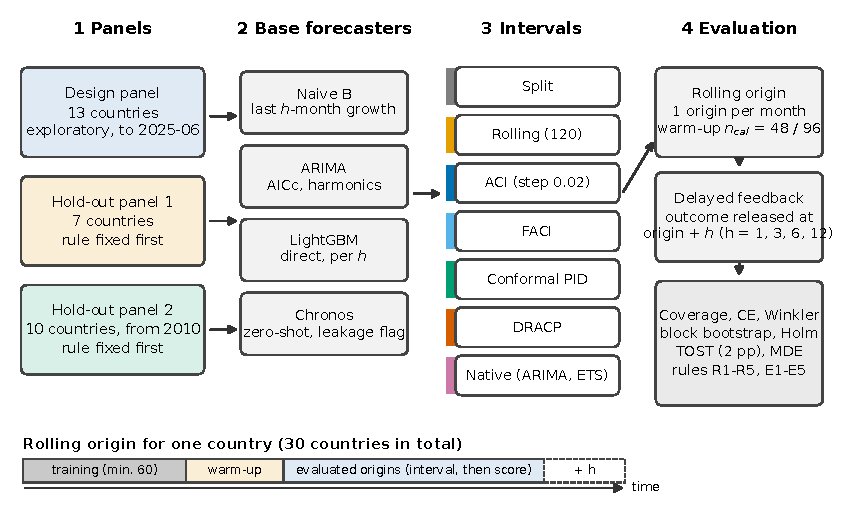
\includegraphics[width=\linewidth]{figures/fig_pipeline.pdf}
\caption{The experimental pipeline: dated and hashed data snapshots, point forecasters, interval methods, evaluation (coverage, calibration error, interval score, block bootstrap, Holm, TOST, minimum detectable difference) and the generation of the paper's figures and tables. The platform and explanation layers are engineering artefacts built on the interval method.}
\label{fig:pipeline}
\end{figure}

\subsection{Pipeline}\label{sec:pipeline}

\paragraph{Data.} Monthly IMF consumer price indices, exchange rates and the Brent crude price are downloaded by Node scripts into dated JSON snapshots whose SHA-256 hashes are recorded (Section~\ref{sec:snapshots} and Appendix~\ref{app:data}). A loader chains the snapshots on the CPI level at their last common month, cuts series into stretches of consecutive months, and labels every evaluated row by sample (exploratory, hold-out or second hold-out) from its target month and country.

\paragraph{Forecasters.} Each base forecaster (naive A and B, ETS, ARIMA, LightGBM, Chronos) is a function of the information dated at or before the forecast origin. Look-ahead is excluded by construction and by tests that corrupt all data after the origin and check that the forecast is unchanged.

\paragraph{Intervals.} The six interval methods consume the point forecast through a streaming interface (\texttt{fit}, \texttt{predict\_one}, \texttt{update\_one}) in which the outcome of the forecast made at origin $j$ is returned only at origin $j+h$ (equation~\eqref{eq:released}). The default is therefore the delayed-feedback setting; the instant-feedback diagnostic is a separate, labelled run.

\paragraph{Evaluation.} Per-row results (forecast, interval bounds, outcome, flags) are summarised into coverage, calibration error, width and interval score, and the contrasts of Section~\ref{sec:contrasts} are computed with the moving-block bootstrap, Holm correction, TOST and the power simulation of Section~\ref{sec:mde}. Robustness analyses (leave-one-country-out, other base models, feedback delay, width) use only existing intervals.

\paragraph{Assets.} The figures and tables of this paper are generated from the committed result tables by a single script, so that every number in a table or figure has a path back to a result file. Numbers quoted in the running text were written from the project's manuscript and its result documents.

\subsection{The platform and the explanation layer (engineering)}\label{sec:platform}

\paragraph{Platform module.} The repository contains a module of the application that serves calibrated inflation intervals for the 13 design economies through a FastAPI endpoint (\texttt{GET /api/v1/inflation/calibrated-forecast}), with a page of the React front end that shows the measured backtest coverage next to the nominal level. The service reads a CPI snapshot and forms the point forecast as $h$ times an exponentially weighted moving average of past monthly log growth (smoothing parameter 0.2). It issues intervals by ACI on absolute residuals over a rolling calibration window of 120 months with step 0.02, with delayed feedback, and requires at least 30 revealed residuals before issuing an interval. The point forecast, the minimum calibration size (30 against the benchmark's warm-up of 48) and the data differ from the benchmark, which uses LightGBM and other base models. The benchmark results therefore bear on the module only through the interval method, and the module's own backtest coverage is displayed to users. ACI was chosen for the module as an adaptive method that is better calibrated than a one-shot calibration and than native intervals, and that is simple to implement and explain; the benchmark did not show it to be better than a rolling window on all panels.

\paragraph{Explanation layer.} A service receives a question about a country and a horizon, calls the platform endpoint as a tool and answers in English, Russian or Kazakh. Its evaluation was specified in the eighth protocol entry before any request was made: 13 countries, 4 horizons, 3 question types and 3 languages give 468 prompts, each answered in two conditions (with the tool result in the context, and without it as an ungrounded baseline), so 936 calls. The metrics are computed by program and not by a judge model: numerical faithfulness, omission rate and coverage overstatement, with Wilson 95\% intervals, and a manual review of 30 answers per language for fluency and terminology; there is no pass threshold. After the protocol entry the harness was changed to call only an OpenAI-compatible endpoint (a LiteLLM proxy, with the model identifier taken from an environment variable); the design of the evaluation described above did not change in this respect. The service and the harness were tested with a deterministic fake client that only exercises the code.

\textbf{The evaluation of the explanation layer has not been run on a real language model, and no result is reported.} The output of the fake client is not a result. No claim of this paper depends on this component, and nothing is claimed about the faithfulness, omissions or overstatements of such a layer.

\section{Datasets and experimental design}\label{sec:data}

\subsection{Sources}

All series are monthly. Consumer price indices (all items) come from the IMF (series \texttt{M.<country>.PCPI\_IX}), obtained through DBnomics for the first snapshot and through the IMF SDMX API for the second. The exchange rate is the monthly average of domestic currency per US dollar (IMF IFS). The Brent crude price is from the IMF primary commodity price series; in the direct API it requires the area code \texttt{G001}. The exchange rate and Brent enter the feature set of the LightGBM forecaster, and the exchange rate defines the stress measure of the secondary analysis.

\subsection{Panels and selection rules}\label{sec:panels}

Table~\ref{tab:panels} summarises the three panels; the selection rules follow.

\begin{table}[t]
\centering
\caption{The three country panels (design, first hold-out, second hold-out): CPI coverage, number of months and number of origins at $h=3$ per country.}
\label{tab:panels}
\small
\fittable{\begin{tabular}{llllrr}
\toprule
Code & Country & CPI from & CPI to & Months & Origins ($h{=}3$) \\
\midrule
\multicolumn{6}{l}{\emph{Design (13)}} \\
BR & Brazil & 2000-01 & 2025-06 & 306 & 193 \\
MX & Mexico & 2000-01 & 2025-06 & 306 & 193 \\
CL & Chile & 2000-01 & 2025-06 & 306 & 193 \\
CO & Colombia & 2000-01 & 2025-06 & 306 & 193 \\
PE & Peru & 2010-01 & 2025-06 & 186 & 73 \\
ZA & South Africa & 2000-01 & 2025-06 & 306 & 193 \\
ID & Indonesia & 2000-01 & 2025-06 & 306 & 193 \\
KZ & Kazakhstan & 2005-01 & 2025-06 & 246 & 133 \\
RU & Russia & 2000-01 & 2025-06 & 286 & 154 \\
AZ & Azerbaijan & 2005-01 & 2025-06 & 246 & 133 \\
UZ & Uzbekistan & 2010-01 & 2025-06 & 186 & 73 \\
NG & Nigeria & 2005-01 & 2025-06 & 246 & 127 \\
MN & Mongolia & 2006-01 & 2025-06 & 234 & 121 \\
\midrule
\multicolumn{6}{l}{\emph{Hold-out 1 (7)}} \\
BO & Bolivia & 2005-01 & 2026-06 & 258 & 145 \\
PY & Paraguay & 2005-01 & 2026-06 & 258 & 145 \\
UY & Uruguay & 2005-01 & 2026-06 & 258 & 145 \\
GH & Ghana & 2000-01 & 2026-06 & 318 & 205 \\
GE & Georgia & 2005-01 & 2026-06 & 258 & 145 \\
KG & Kyrgyzstan & 2003-01 & 2026-06 & 282 & 169 \\
AO & Angola & 2002-01 & 2026-06 & 294 & 181 \\
\midrule
\multicolumn{6}{l}{\emph{Hold-out 2 (10)}} \\
ZM & Zambia & 2010-01 & 2026-06 & 198 & 89 \\
AM & Armenia & 2010-01 & 2026-06 & 198 & 88 \\
TZ & Tanzania & 2010-01 & 2026-06 & 198 & 87 \\
UG & Uganda & 2010-01 & 2026-06 & 198 & 88 \\
KE & Kenya & 2010-01 & 2026-06 & 198 & 88 \\
IQ & Iraq & 2010-01 & 2026-06 & 198 & 88 \\
BW & Botswana & 2010-01 & 2026-06 & 198 & 87 \\
NA & Namibia & 2010-01 & 2026-06 & 198 & 86 \\
MZ & Mozambique & 2010-01 & 2026-06 & 198 & 89 \\
CI & Cote d'Ivoire & 2010-01 & 2026-06 & 198 & 88 \\
\bottomrule
\end{tabular}
}
\end{table}

\paragraph{Design countries (13).} Core long-history group: Brazil, Mexico, Chile, Colombia, Peru, South Africa, Indonesia. Regional group: Kazakhstan, Russia, Azerbaijan, Uzbekistan. Control group: Nigeria, Mongolia. These countries were used to shape the design (the stress rule, the start date, the contrasts and the horizons). No export-share rule was applied to select them; the measured classification is in Section~\ref{sec:scope}.

\paragraph{First hold-out panel (7).} Bolivia, Paraguay, Uruguay, Ghana, Georgia, Kyrgyzstan, Angola. The candidate list (14 names in a fixed order) and the eligibility rule were written in the fetching script before any forecast was computed for these countries. The rule required at least 220 months of IMF monthly CPI and of exchange rate per US dollar within 2000-01 to 2026-06, with at most 3 missing CPI months, and the first 10 eligible candidates were to be kept. Only 7 candidates met the rule (six candidates start in 2009 or 2010 and one has no CPI series), so the panel has 7 countries and the rule was not relaxed. Target months run from 2009-02 to 2026-06, and all months of these countries are labelled \texttt{holdout}.

\paragraph{Second hold-out panel (10), extension.} Zambia, Armenia, Tanzania, Uganda, Kenya, Iraq, Botswana, Namibia, Mozambique, C\^ote d'Ivoire. The candidate list and the eligibility rule were written before any forecast of any kind was computed for these countries (eighth protocol entry, Section~\ref{sec:extension}). The rule required at least 170 months of IMF monthly CPI and of exchange rate per US dollar within 2010-01 to 2026-06, with at most 3 missing CPI months; the first 10 eligible candidates were kept, and six more candidates were eligible but came after the first 10 and were not used. Each series has 198 months from 2010-01. Six of these countries were candidates of the first hold-out rule and did not qualify under its 220-month requirement; no country is in two panels. All target months are labelled \texttt{holdout2}. After the 60-month training minimum and a warm-up of 48 there are 89 pooled calendar months at $h=3$ and 83 at $h=6$, and after a warm-up of 96 there are 41 and 35.

\subsection{Snapshots}\label{sec:snapshots}

Dated snapshots with SHA-256 hashes were taken from the IMF: two for the design countries and one file for each hold-out panel (Appendix~\ref{app:data}). The first snapshot (CPI, exchange rate and Brent for the 13 design countries from DBnomics, indexed 2025-08-31) and the second (data from 2024-01 onwards fetched directly from the IMF SDMX API after the protocol was committed) overlap from 2024-01 to 2025-05. The overlap is identical for the exchange rate, Brent and CPI except for three differences recorded in the protocol: a constant rebasing of the index level for Kazakhstan (ratio 0.477) and Nigeria (ratio 0.131), small revisions for Russia (up to 0.07 percent) and Mongolia (up to 0.05 percent), and a methodology break in the Nigerian series at 2025-01.

\subsection{Rebasing and the Nigerian methodology break}

Because the two snapshots use different index bases, the loader chains them on the CPI level at the last month they have in common. The earlier snapshot wins on overlap, and later months are rescaled by a constant factor, so growth rates are unaffected. An early version of the loader merged the snapshots without rescaling and produced a false 74 percent fall in the Kazakhstani index; this was found and fixed before the run, and a regression test now checks that no country has a monthly log jump above 0.15 at the junction. For Nigeria, the CPI index falls from 113.9 to 110.7 in rebased terms between 2024-12 and 2025-01, which reflects a change in methodology and not a price movement. Months from 2025-01 are therefore not appended and the Nigerian series ends at 2024-12. Russia has 30 missing CPI months; its series is cut into stretches of consecutive months and only stretches of at least 60 months are used. Series that start later than 2000 (Kazakhstan, Azerbaijan and Nigeria from 2005, Mongolia from 2006, Uzbekistan and Peru from 2010) enter once they have 60 months of history.

\subsection{Exploratory and confirmatory samples}\label{sec:samples}

The label of each evaluated row depends on its target month. Target months before 2025-07 are labelled exploratory. Target months from 2025-07 on the 13 design countries are labelled confirmatory in the code, but with at most about 16 months per country there are two or three independent blocks, so these months cannot carry a claim. The main confirmatory pool became the 7 hold-out countries, and the extension adds the 10 countries of the second hold-out panel. The run on the post-2025-06 months of the 13 countries is degenerate and is not used (Section~\ref{sec:confirm13}). Exploratory results (target months up to 2025-05 or 2025-06 for the design countries) and the hold-out results are kept separate throughout, and no threshold or window was tuned on the hold-out data or to raise a result.

\subsection{Interval methods and base models}

Table~\ref{tab:methods} lists the interval methods, the base forecasters and the evaluation settings. The nominal level is 0.90; the primary warm-up is $n_{\mathrm{cal}}=48$ residuals and a sensitivity run uses $n_{\mathrm{cal}}=96$, applied to all methods and not promoted to the primary configuration.

\begin{table}[t]
\centering
\caption{Interval methods, base forecasters and evaluation settings (nominal level 0.90; rolling window 120; ACI step 0.02).}
\label{tab:methods}
\small
\fittable{\begin{tabular}{p{0.15\linewidth}p{0.45\linewidth}p{0.32\linewidth}}
\toprule
Item & Description & Key settings \\
\midrule
\multicolumn{3}{l}{\emph{Interval methods (nominal level 0.90, $\alpha=0.10$)}} \\
Split & Quantile of absolute residuals on the warm-up window; fixed, never updated & Warm-up $n_{\mathrm{cal}}=48$ (primary) or 96 \\
Rolling & Quantile of the most recent absolute residuals & Window 120 residuals \\
ACI & Rolling window; quantile level moved online after each released outcome & Step 0.02, window 120 \\
FACI & Aggregation of ACI experts with several step sizes & Package defaults (\texttt{dracp}) \\
Conformal PID & Error-integrator and scorecaster control of the quantile & Package defaults (\texttt{dracp}) \\
DRACP & Regime-aware calibration with FACI control of the level & Calibration window 120, target window 24, decay 0.985, adaptive bandwidth (grid), 3 regimes \\
Native & Parametric intervals of the base model (ARIMA: Gaussian from $\psi$-weights; ETS: simulation) & ETS: 400 simulated paths \\
\midrule
\multicolumn{3}{l}{\emph{Base point forecasters (cumulative $h$-month log growth)}} \\
Naive B & Last observed cumulative $h$-month growth & No parameters \\
ARIMA & ARMA$(p,q)$ with constant and two annual harmonics on monthly inflation; $h$ forecasts summed & $p,q\in\{0,1,2\}$ by AICc every 12 origins \\
LightGBM & Direct forecast, one model per horizon & 200 trees, learning rate 0.05, 8 leaves, subsample 0.8, column sample 0.8, refit every 3 origins \\
Chronos & Pretrained model used zero-shot on monthly inflation; $h$ median forecasts summed & \texttt{chronos-bolt-tiny}, context 2048, no covariates \\
\midrule
\multicolumn{3}{l}{\emph{Evaluation}} \\
Rolling origin & One origin per month, expanding training window; outcome released $h$ months after the origin & Minimum 60 months of history; horizons 1, 3, 6, 12 \\
Calibration error & Mean over countries of $|\mathrm{coverage}-0.90|$ & Equal weight per country \\
Bootstrap & Moving blocks of calendar months, resampled jointly across countries & Block length $\max(h,12)$, 2000 replicates, 95\% percentile interval \\
Multiplicity & Holm over the primary family of four contrasts per base model & ACI $-$ rolling and DRACP $-$ ACI at $h=3,6$ \\
TOST & Equivalence of DRACP and ACI & Margin 2 pp of CE \\
MDE (R5, E5) & Simulated minimum detectable difference at power 0.80 & Undefined or above 7 pp: inconclusive \\
\bottomrule
\end{tabular}
}
\end{table}

\subsection{What ``pre-specified'' means and the sequence of events}\label{sec:prespec}

The protocol and the shock definition are committed documents in the project repository. Changes are logged in their ``Changes'' sections with a date and a reason. ``Pre-specified'' in this paper means that a rule was committed to the repository before the run it governs. It does not mean registration in an external registry, and the order of events is not independently timestamped: the author is a single person, all entries are dated 2026-11-18 or 2026-11-19, and the order is attested only by a commit history kept by the same person. The decision rules R1--R5 were written after the exploratory results at both warm-ups were known, so they were set by an author who knew how the design countries behaved. The sequence was as follows.
\begin{enumerate}
\item \textbf{Shock rule frozen} (document dated 2026-11-18), before any forecast was computed. Validity checks were run afterwards (Section~\ref{sec:shockvalid} and Appendix~\ref{app:extra}).
\item \textbf{Protocol draft 1}, written before any forecast or interval had been computed. A committee review scored it 5.5 out of 10, and the claim hierarchy, FACI and conformal PID, a reproduction tolerance, a block length of at least $h$, reduced primary tests and a threshold for the minimum detectable difference were added before any forecast. A second entry added the second snapshot and the Nigerian break and restricted confirmatory analysis to the pooled panel. A partial reproduction of DRACP was recorded and the topic was fixed.
\item \textbf{Third entry and the exploratory run.} Implementation decisions of the engine (start 2000-01, warm-up 48, window 120, ACI step 0.02, snapshot chaining) were fixed before results existed. The first run was exploratory only (target months up to 2025-06), so that no target month from 2025-07 could enter.
\item \textbf{Fourth entry: amendments after the exploratory result and before any hold-out forecast.} Pooled-coverage contrasts were replaced by calibration error as the primary outcome; the reference changed from split to rolling conformal; DRACP against ACI became an equivalence question with a 2~pp margin; a fair DRACP sensitivity with warm-up 96 was added; the 7 hold-out countries became the main confirmatory pool; block length became at least 12; and the stress analysis was kept exploratory. The text of the entry states that the changes are motivated by logical defects of the design and not by significance. These amendments were made after the exploratory results were known.
\item \textbf{Fifth entry: hold-out run specification and decision rules R1--R5}, before any forecast was computed for the 7 hold-out countries. The runs were (A) warm-up 48 (primary), (B) warm-up 96 (sensitivity) and (C) an instant-feedback diagnostic at $h=12$. The entry states that none of the rules is changed after the result is seen.
\item \textbf{Hold-out run}, the first and only look at the 7 countries.
\item \textbf{Sixth entry: robustness analyses S1--S5}, written after the hold-out result and before they were computed. They are secondary, do not replace R1--R5, and no threshold was changed.
\item \textbf{Seventh entry (post hoc): additions S6 (Kazakhstan alone) and S7 (native intervals)}, requested by a review of the manuscript draft, recorded before they were computed and computed from existing outputs only. They are post hoc, descriptive or secondary, and not part of the pre-specified family.
\item \textbf{Eighth entry: the extension} (Section~\ref{sec:extension}), specifying the second hold-out panel, the Chronos forecaster, the rules E1--E5 and the evaluation of the explanation layer. The specification was written after R1--R5 had been applied and after the R2 outcome on the first hold-out panel and the robustness results were known; it does not change R1--R5 or any earlier result.
\end{enumerate}
Commit hashes for each step are listed in Appendix~\ref{app:changes}.

\subsection{Procedural boundary}\label{sec:boundary}

The hold-out countries are untouched with respect to countries only. They are independent of the design sample by country, but they share calendar months with it (the global shocks of 2020 to 2022 fall in both samples). The set of methods, the form of the contrasts, the horizons, the 2~pp margin and the 3~pp and 7~pp thresholds were chosen on the 13 design countries. The author had also seen the post-2025-06 months of the 13 design countries before the amendments. The hold-out evaluation is therefore a test on new countries and not a fully blind test of the design. The second hold-out panel is independent of both earlier samples by country, but it too shares calendar months with them (2010 to 2026), and its rules E1--E5 were written by an author who knew every earlier result, including the R2 outcome on the first hold-out panel. It is a replication on new countries and not a blind test.

\subsection{The decision rules R1--R5}\label{sec:rules}

The rules apply to the base model LightGBM, the primary family with Holm correction over four tests, pooled over the 7 hold-out countries, with a block length of 12. They are reproduced in Table~\ref{tab:rules} together with the extension rules E1--E5, and their recorded outcomes are discussed in Section~\ref{sec:results}. In words:
\begin{itemize}
\item \textbf{R1 (replication of the secondary result):} ACI is better calibrated than split if the CE difference ACI minus split is negative with Holm $p<0.05$ at both $h=3$ and $h=6$.
\item \textbf{R2 (does adaptivity help beyond a rolling window):} ``ACI improves on rolling'' only if ACI minus rolling is negative with Holm $p<0.05$ at the horizon; otherwise ``not shown''.
\item \textbf{R3 (DRACP against ACI):} ``no advantage, equivalent within 2~pp'' only if equivalence holds at both warm-up sizes; ``DRACP better'' only if DRACP minus ACI is negative with Holm $p<0.05$ at both warm-ups; otherwise ``inconclusive''.
\item \textbf{R4 (delayed feedback explains the $h=12$ shortfall):} supported if the mean coverage of ACI with instant feedback exceeds the delayed one by at least 3~pp on the hold-out panel.
\item \textbf{R5 (power):} a contrast whose minimum detectable difference is undefined or above 7~pp is reported as inconclusive regardless of its $p$-value.
\end{itemize}

\begin{table}[t]
\centering
\caption{Decision rules R1--R5 and extension rules E1--E5 as pre-specified, with their recorded outcomes.}
\label{tab:rules}
\small
\fittable{\begin{tabular}{p{0.05\linewidth}p{0.36\linewidth}p{0.11\linewidth}p{0.38\linewidth}}
\toprule
Rule & Statement & Status & Outcome as recorded \\
\midrule
\multicolumn{4}{l}{\emph{First hold-out panel (7 countries, LightGBM, Holm over four tests)}} \\
R1 & ACI better calibrated than split: ACI $-$ split negative with Holm $p<0.05$ at $h=3$ and $h=6$ & Not met & Not met in the primary run (warm-up 48); met at warm-up 96 (sensitivity run, not promoted) \\
R2 & ACI improves on rolling: ACI $-$ rolling negative with Holm $p<0.05$ & Not shown & Not shown (MDE undefined, inconclusive); Holm $p$ 0.35 and 1.0 at warm-up 48 \\
R3 & DRACP versus ACI: equivalence within 2 pp at both warm-ups, or DRACP better with Holm $p<0.05$ at both & Inconclusive & Equivalent at warm-up 48, not shown at 96; the verdict is not stable \\
R4 & Delayed feedback explains the $h=12$ shortfall: ACI coverage with instant feedback higher by at least 3 pp & Not met & Not met: +2.4 pp against the 3 pp threshold (coverage 0.884 delayed, 0.908 instant) \\
R5 & Power: MDE undefined or above 7 pp is inconclusive regardless of $p$ & Inconclusive & All four primary contrasts inconclusive (MDE undefined on the full hold-out sample) \\
\midrule
\multicolumn{4}{l}{\emph{Extension, second hold-out panel (10 countries, four base models, warm-up 48 primary)}} \\
E1 & Replication of R1, R2, R3 on new countries, same rule and direction & Partly & R1 met for all four base models at both horizons (not met at warm-up 96); R2 met at $h=3$ for LightGBM, ARIMA and naive B and at $h=6$ for ARIMA and naive B (Chronos at $h=3$ inconclusive under E5); R3 inconclusive \\
E2 & Dependence on the base model: contrasts side by side, no threshold & Descriptive & R1 and R3 do not depend on the base model; R2 at $h=6$ does (ARIMA, naive B met; LightGBM, Chronos not met) \\
E3 & Point accuracy of Chronos: relative MAE with bootstrap interval, descriptive & Descriptive & Relative MAE of Chronos on clean months 0.774, 0.699, 0.654, 0.895 at $h=1,3,6,12$; no interval favours LightGBM or ARIMA \\
E4 & Leakage: accuracy claims only from target months from 2025-01 & Applied & 22 months, 567 country-month cells per horizon, 30 countries; the 2025-01 cutoff is an assumption, not verified \\
E5 & Power: MDE undefined or above 7 pp is inconclusive & Applied & MDE of ACI $-$ rolling 1.2 to 6.6 pp at warm-up 48, undefined for Chronos at $h=3$; undefined for every DRACP $-$ ACI contrast and for all contrasts at warm-up 96 \\
\bottomrule
\end{tabular}
}
\end{table}

\subsection{The extension: second hold-out panel, Chronos and the rules E1--E5}\label{sec:extension}

The eighth protocol entry (2026-11-19) specifies the extension before any forecast, request or evaluation of it was computed, and before any forecast of any kind was computed for the 10 countries of the second hold-out panel. It does not change R1--R5.

\paragraph{Runs.} All extension runs start at 2010-01. (E-A) Base models LightGBM, ARIMA, naive B and Chronos on the second hold-out panel at warm-up 48 (primary) and warm-up 96 (sensitivity, not promoted). (E-B) The four base models were run on the 13 design countries and the 7 first hold-out countries as a secondary analysis; calibration contrasts were analysed only for LightGBM and Chronos, which narrows the E-B analysis of the protocol (a deviation). Because these runs start in 2010 and not in 2000, their numbers differ from those of the earlier sections and are not comparable with them cell by cell.

\paragraph{Rules.} The rules are applied separately for each base model, with the CE family of the protocol (ACI minus rolling and DRACP minus ACI at $h=3$ and $h=6$, Holm over four tests; ACI minus split and ACI minus native secondary).
\begin{itemize}
\item \textbf{E1, replication on new countries.} A statement of R1, R2 or R3 is ``replicated'' for a base model only if the same rule is met in the same direction; otherwise it is reported as not replicated or inconclusive. Results at warm-up 96 are a sensitivity analysis and are not promoted.
\item \textbf{E2, dependence on the base model.} The contrasts for the four base models are reported side by side, without a threshold.
\item \textbf{E3, point accuracy of Chronos.} Mean absolute error relative to naive B per horizon, next to ARIMA, ETS and LightGBM, with a block-bootstrap 95\% interval; descriptive.
\item \textbf{E4, leakage.} Claims about the accuracy of Chronos are drawn only from the target months from 2025-01, pooled over all 30 countries, and the thinness of that sample is stated. Calibration contrasts for Chronos are reported on all months with the flag.
\item \textbf{E5, power.} A contrast whose minimum detectable difference is undefined or above 7~pp is inconclusive.
\end{itemize}

\paragraph{Multiplicity.} The Holm correction is applied within each base model (four tests). It is not applied across the four base models, and the four base models are evaluated on the same countries and months, so their results are not independent replications. No statement in this paper rests on pooling the four.

\paragraph{Implementation note and deviations.} The first attempt to analyse the new panel failed because the country code NA (Namibia) was read as a missing value by the CSV reader; the reader was fixed with a regression test, the forecasts were not affected and were not recomputed, and only the analysis step was repeated. Two deviations from the protocol are stated. (1) Calibration contrasts for the earlier 20 countries were analysed only for LightGBM and Chronos although four base models were run. (2) The protocol asks for relative mean absolute error (E3) with bootstrap intervals next to ARIMA, ETS and LightGBM; the all-months accuracy table has no intervals and no ETS, because ETS was not part of the extension runs, while the clean-month analysis has intervals against LightGBM, ARIMA and naive B.

\subsection{Validity of the shock rule and why stress is secondary}\label{sec:shockvalid}

A committee review scored the frozen exchange-rate-based shock rule 5.5 out of 10, objecting that an exchange-rate flag measures currency turbulence and not an inflation shock. Two checks were run on the 13 design countries; they are exploratory because the same countries shaped the design. With the discrete label, the share of the top-decile one-step errors of a naive forecast that falls inside shock windows exceeded the share of shock months by a lift of 1.49 to 1.87, below the committee's bar of 2 (Appendix~\ref{app:extra}). With the continuous stress variable, the pooled within-country rank correlation with the naive one-step error was 0.075 (permutation $p=0.001$) for origin stress over all months and 0.050 ($p=0.0495$) since 2015-09, and the relation is not monotone. Because the association is weak and concentrated in the upper tail, the main contribution does not depend on shocks. Parameters of the rule were not tuned to raise the lift, and the upper decile was not promoted to a primary threshold after the fact. Kazakhstan has fewer than 10 independent episodes after 2015-09 and is therefore a descriptive case inside a pooled panel, not a stand-alone inferential unit.

\subsection{Commodity dependence of the panel}\label{sec:scope}

``Commodity-dependent'' is defined by a measured external criterion: the share of commodities in merchandise exports of at least 60\% (strong) or 40--60\% (moderate), averaged over 2021--2023 (UNCTAD, \emph{The State of Commodity Dependence 2025}; second window 2012--2014). No export-share rule was applied to select the countries. The classification was applied afterwards, so it is post hoc and descriptive, and part of the shares had been read before the criterion was written down (tenth protocol entry). Table~\ref{tab:commodity} shows that 27 of the 30 economies qualify at 60\%. Mexico, Indonesia (62.4\% in 2012--2014) and Georgia do not and are kept as comparison cases; Uruguay (82.9\%) is strongly dependent. The hold-out sets were determined by IMF data availability under fixed rules: 7 of 14 candidates qualified for the first panel, and the first 10 eligible candidates formed the second panel. With three non-qualifying countries the study cannot compare commodity-dependent with other economies, and the descriptive calibration error by class is inconclusive.

\begin{table}[t]
\centering
\caption{Commodity dependence of the three panels (UNCTAD, share of commodities in merchandise exports, average 2021--2023; classification applied post hoc).}
\label{tab:commodity}
\small
\fittable{\begin{tabular}{lrrrrl}
\toprule
Panel & Countries & $\geq 60\%$ & 40--60\% & $<40\%$ & Not qualifying at 60\% (share, \%) \\
\midrule
Design & 13 & 11 & 1 & 1 & Mexico (18.2), Indonesia (55.9) \\
Hold-out 1 & 7 & 6 & 1 & 0 & Georgia (46.4) \\
Hold-out 2 & 10 & 10 & 0 & 0 & none \\
All & 30 & 27 & 2 & 1 & \\
\bottomrule
\end{tabular}}
\end{table}

\section{Results}\label{sec:results}

All results use LightGBM as base model and nominal level 0.90, unless stated otherwise. A negative CE contrast means that the first method is better calibrated. The exploratory results carry no confirmatory claim. The word ``significant'' is not used for any result outside the pre-specified family, and unadjusted $p$-values are given as descriptive. Sections~\ref{sec:explor} to~\ref{sec:width} concern the design panel and the first hold-out panel; Section~\ref{sec:panel2} reports the extension (second hold-out panel, four base models) and is kept apart because the panel, the base models and the start date differ; Section~\ref{sec:ablation} collects the ablation analyses (base model, warm-up, feedback delay, native intervals and Chronos accuracy).

\subsection{Calibration of adaptive methods against the baselines}\label{sec:explor}

Figure~\ref{fig:coverage_h} shows pooled coverage by method and horizon for the panels of the study, and Figure~\ref{fig:ce_bars} the calibration error. The exploratory run covers 13 units, origins from 2000-01 and target months to 2025-06, with warm-up 48. Pooled coverage at $h=1,3,6,12$ is 0.946, 0.937, 0.917 and 0.864 for split conformal; 0.917, 0.916, 0.900 and 0.869 for rolling; and 0.908, 0.906, 0.899 and 0.864 for ACI (the number of unit-months is 2024, 1972, 1894 and 1738; the full table is in Appendix~\ref{app:extra}). Split conformal over-covers at short horizons, so that a lower coverage there is closer to nominal. Bootstrap 95 percent intervals are wide: for ACI they are \ci{0.879}{0.930} at $h=3$ and \ci{0.797}{0.914} at $h=12$.

\begin{figure}[t]
\centering
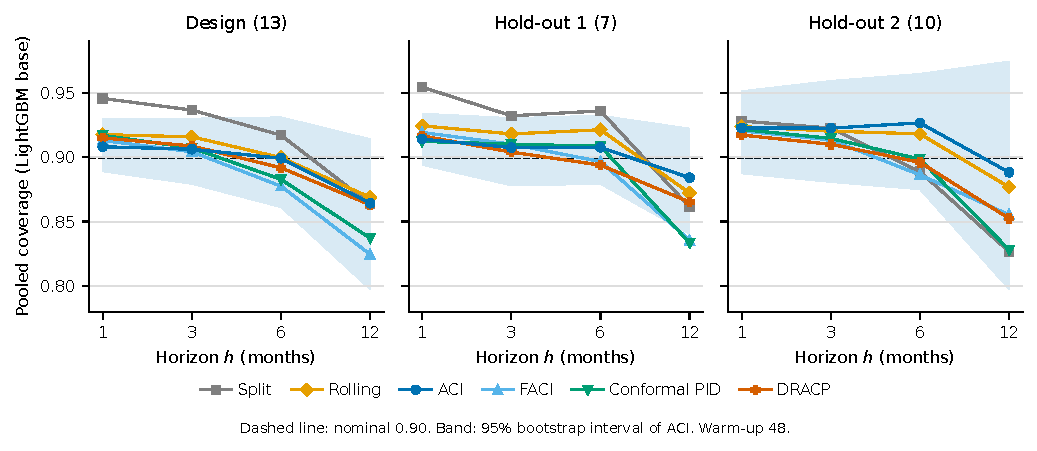
\includegraphics[width=\linewidth]{figures/fig_coverage_h.pdf}
\caption{Pooled empirical coverage by horizon and interval method for each panel (LightGBM base), against the nominal level 0.90.}
\label{fig:coverage_h}
\end{figure}

\begin{figure}[t]
\centering
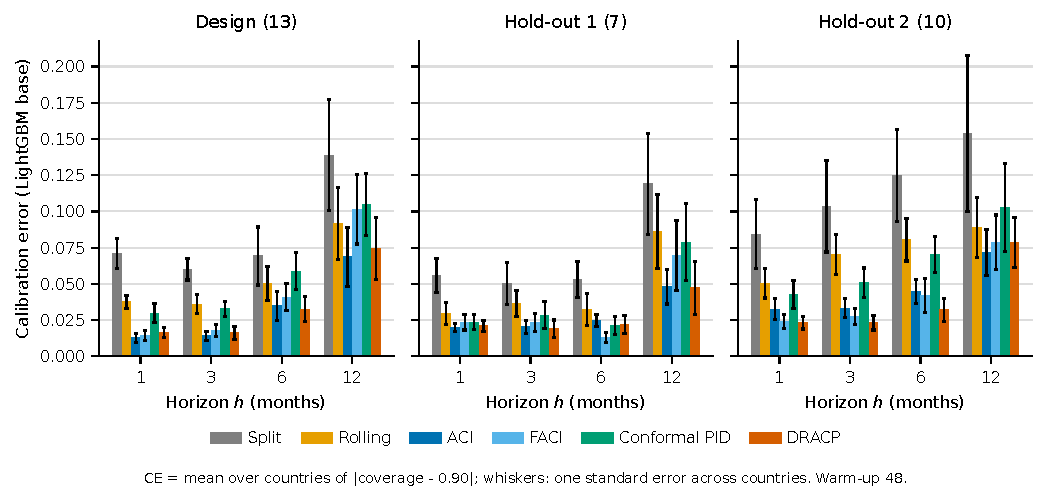
\includegraphics[width=\linewidth]{figures/fig_ce_bars.pdf}
\caption{Calibration error (mean over countries of $|\text{coverage}-0.90|$) by interval method and horizon for each panel (LightGBM base).}
\label{fig:ce_bars}
\end{figure}

Tables~\ref{tab:ce_expl} and~\ref{tab:ce_ho1} give the calibration error on the design panel and on the first hold-out panel. In the exploratory data the CE of ACI at $h=1,3,6,12$ is 0.013, 0.014, 0.035 and 0.069, against 0.038, 0.036, 0.050 and 0.091 for rolling and 0.071, 0.060, 0.069 and 0.139 for split. On the first hold-out panel it is 0.020, 0.020, 0.025 and 0.048 for ACI, 0.029, 0.036, 0.032 and 0.086 for rolling, and 0.056, 0.050, 0.053 and 0.119 for split; DRACP has 0.021, 0.019, 0.022 and 0.047, FACI 0.024, 0.023, 0.013 and 0.070, and conformal PID 0.024, 0.028, 0.021 and 0.079.

\begin{table}[t]
\centering
\caption{Calibration error by base model, interval method and horizon, design panel (13 countries, exploratory, warm-up 48).}
\label{tab:ce_expl}
\small
\fittable{\begin{tabular}{llrrrr}
\toprule
Base model & Interval & $h{=}1$ & $h{=}3$ & $h{=}6$ & $h{=}12$ \\
\midrule
LightGBM & Split & 0.071 & 0.060 & 0.069 & 0.139 \\
 & Rolling & 0.038 & 0.036 & 0.050 & 0.091 \\
 & ACI & 0.013 & 0.014 & 0.035 & 0.069 \\
 & FACI & 0.014 & 0.018 & 0.041 & 0.101 \\
 & Conformal PID & 0.030 & 0.033 & 0.059 & 0.105 \\
 & DRACP & 0.016 & 0.016 & 0.033 & 0.074 \\
\midrule
ARIMA & Split & 0.064 & 0.064 & 0.098 & 0.148 \\
 & Rolling & 0.031 & 0.032 & 0.058 & 0.096 \\
 & ACI & 0.010 & 0.015 & 0.026 & 0.079 \\
 & FACI & 0.017 & 0.023 & 0.029 & 0.102 \\
 & Conformal PID & 0.027 & 0.020 & 0.046 & 0.099 \\
 & DRACP & 0.012 & 0.015 & 0.021 & 0.072 \\
 & Native & 0.047 & 0.066 & 0.089 & 0.137 \\
\midrule
Naive B & Split & 0.057 & 0.069 & 0.073 & 0.171 \\
 & Rolling & 0.031 & 0.035 & 0.043 & 0.100 \\
 & ACI & 0.012 & 0.016 & 0.024 & 0.057 \\
 & FACI & 0.017 & 0.018 & 0.039 & 0.124 \\
 & Conformal PID & 0.025 & 0.021 & 0.036 & 0.113 \\
 & DRACP & 0.017 & 0.017 & 0.028 & 0.071 \\
\midrule
ETS & Native & 0.044 & 0.051 & 0.064 & 0.116 \\
\bottomrule
\end{tabular}
}
\end{table}

\begin{table}[t]
\centering
\caption{Calibration error by base model, interval method and horizon, first hold-out panel (7 countries, warm-up 48).}
\label{tab:ce_ho1}
\small
\fittable{\begin{tabular}{llrrrr}
\toprule
Base model & Interval & $h{=}1$ & $h{=}3$ & $h{=}6$ & $h{=}12$ \\
\midrule
LightGBM & Split & 0.056 & 0.050 & 0.053 & 0.119 \\
 & Rolling & 0.029 & 0.036 & 0.032 & 0.086 \\
 & ACI & 0.020 & 0.020 & 0.025 & 0.048 \\
 & FACI & 0.023 & 0.023 & 0.013 & 0.070 \\
 & Conformal PID & 0.024 & 0.028 & 0.021 & 0.079 \\
 & DRACP & 0.021 & 0.019 & 0.022 & 0.047 \\
\midrule
ARIMA & Split & 0.067 & 0.065 & 0.061 & 0.106 \\
 & Rolling & 0.039 & 0.043 & 0.040 & 0.069 \\
 & ACI & 0.014 & 0.013 & 0.024 & 0.040 \\
 & FACI & 0.019 & 0.010 & 0.029 & 0.084 \\
 & Conformal PID & 0.029 & 0.037 & 0.034 & 0.083 \\
 & DRACP & 0.020 & 0.011 & 0.027 & 0.051 \\
 & Native & 0.053 & 0.058 & 0.062 & 0.073 \\
\midrule
Naive B & Split & 0.063 & 0.049 & 0.135 & 0.175 \\
 & Rolling & 0.039 & 0.030 & 0.061 & 0.052 \\
 & ACI & 0.015 & 0.021 & 0.030 & 0.032 \\
 & FACI & 0.026 & 0.020 & 0.036 & 0.079 \\
 & Conformal PID & 0.030 & 0.027 & 0.050 & 0.070 \\
 & DRACP & 0.024 & 0.024 & 0.032 & 0.055 \\
\midrule
ETS & Native & 0.056 & 0.035 & 0.048 & 0.053 \\
\bottomrule
\end{tabular}
}
\end{table}

The exploratory contrasts of the primary family are, at warm-up 48, ACI minus rolling $-2.2$~pp at $h=3$ and $-1.5$~pp at $h=6$ with unadjusted $p$-values 0.030 and 0.020 but Holm-adjusted 0.090 and 0.078, so neither survives the correction for the family. ACI minus split (secondary) was $-4.6$~pp at $h=3$ (95\% interval \ci{-5.0}{-1.4}, unadjusted $p=0.001$) and $-3.4$~pp at $h=6$ ($p=0.0025$). DRACP minus ACI was $+0.2$~pp and $-0.2$~pp, within noise. Equivalence within 2~pp was shown at warm-up 48 (maximum one-sided $p$ 0.0085 at $h=3$ and 0.0135 at $h=6$) and not shown at warm-up 96 (0.128 and 0.146). At warm-up 96, in the exploratory data, DRACP was wider than ACI: its Winkler score was higher by 33.2 percent at $h=3$ (95\% interval \ci{12.1}{75.9}, unadjusted $p=0.049$) and 19.9 percent at $h=6$ (\ci{6.8}{46.2}, $p=0.054$). Equivalence in the exploratory data is therefore not stable across warm-up sizes.

Further exploratory observations. At $h=3$ split coverage ranges from 0.822 (Peru) and 0.827 (Kazakhstan) to 1.000 (Indonesia), while ACI ranges from 0.886 to 0.934 (Figure~\ref{fig:country_cov}); at $h=12$ ACI coverage ranges from 0.655 (Peru) and 0.716 (Nigeria) to 1.000 (Uzbekistan). At $h=12$ pooled coverage is below nominal for every method (0.825 to 0.869) and the adaptive methods do not repair it; the bootstrap interval of ACI, \ci{0.797}{0.914}, includes 0.90, and so do those of DRACP, rolling and split (upper limits 0.918, 0.920 and 0.915), but those of FACI and conformal PID do not (0.876 and 0.897). Mean absolute error relative to naive B was 0.74 (ARIMA), 0.72 (ETS) and 0.74 (LightGBM) at $h=3$, 0.75, 0.76 and 0.75 at $h=6$, and 0.86, 0.93 and 0.91 at $h=12$.

\subsection{First hold-out panel and the decision rules R1--R5}\label{sec:holdout}

The hold-out run covers 7 countries, target months 2009-02 to 2026-06, with 205 and 199 pooled months at $h=3$ and $h=6$ for run A (warm-up 48) and 157 and 151 for run B (warm-up 96); the number of unit-months in run A is 1163, 1135, 1093 and 1009 at $h=1,3,6,12$. Pooled coverage in run A at $h=1,3,6,12$ is 0.954, 0.932, 0.936 and 0.861 for split, 0.924, 0.918, 0.921 and 0.872 for rolling, 0.914, 0.907, 0.908 and 0.884 for ACI, 0.919, 0.910, 0.897 and 0.835 for FACI, 0.912, 0.910, 0.909 and 0.833 for conformal PID, and 0.917, 0.904, 0.894 and 0.865 for DRACP (Appendix~\ref{app:extra}). At $h=12$ the pooled coverage of every method is below 0.90 (0.833 to 0.884); the bootstrap upper limits for ACI, DRACP, rolling and split (0.923, 0.901, 0.918 and 0.919) do not exclude 0.90, those of FACI and conformal PID (0.885 and 0.884) do. Table~\ref{tab:contrasts} gives the calibration-error contrasts and Table~\ref{tab:tost} the equivalence tests; the decision rules are applied as pre-specified.

\begin{table}[t]
\centering
\caption{Primary-family calibration-error contrasts by panel and base model: $T$ (pp of CE), 95\% block-bootstrap interval, Holm-adjusted $p$, minimum detectable difference (MDE) and verdict under the power rule.}
\label{tab:contrasts}
\small
\fittable{\begin{tabular}{llcllrrrl}
\toprule
Panel & Base & $h$ & Contrast & $T$ (pp) & 95\% CI & Holm $p$ & MDE (pp) & Verdict \\
\midrule
Design (13) & LightGBM & 3 & ACI $-$ rolling & $-$2.2 & [$-$2.7, +0.1] & 0.090 & -- & Inconclusive \\
 &  & 6 & ACI $-$ rolling & $-$1.5 & [$-$2.1, $-$0.1] & 0.078 & -- & Inconclusive \\
 &  & 3 & DRACP $-$ ACI & +0.2 & [$-$1.2, +1.0] & 1.000 & -- & Inconclusive \\
 &  & 6 & DRACP $-$ ACI & $-$0.2 & [$-$2.0, +1.3] & 1.000 & -- & Inconclusive \\
\midrule
Hold-out 1 (7) & LightGBM & 3 & ACI $-$ rolling & $-$1.6 & [$-$3.0, +0.5] & 0.350 & -- & Inconclusive \\
 &  & 6 & ACI $-$ rolling & $-$0.7 & [$-$2.8, +1.3] & 1.000 & -- & Inconclusive \\
 &  & 3 & DRACP $-$ ACI & $-$0.1 & [$-$1.2, +0.9] & 1.000 & -- & Inconclusive \\
 &  & 6 & DRACP $-$ ACI & $-$0.3 & [$-$1.4, +1.7] & 1.000 & -- & Inconclusive \\
\midrule
Design (13), from 2010 & LightGBM & 3 & ACI $-$ rolling & $-$2.1 & [$-$2.9, +0.5] & 0.216 & -- & Inconclusive \\
 &  & 6 & ACI $-$ rolling & $-$2.0 & [$-$3.1, +0.5] & 0.216 & -- & Inconclusive \\
 &  & 3 & DRACP $-$ ACI & $-$0.5 & [$-$1.6, +1.3] & 0.654 & -- & Inconclusive \\
 &  & 6 & DRACP $-$ ACI & +1.9 & [$-$1.0, +5.5] & 0.654 & -- & Inconclusive \\
\midrule
Design (13), from 2010 & Chronos & 3 & ACI $-$ rolling & $-$1.9 & [$-$2.3, +0.9] & 0.363 & -- & Inconclusive \\
 &  & 6 & ACI $-$ rolling & $-$2.0 & [$-$2.5, +0.8] & 0.358 & -- & Inconclusive \\
 &  & 3 & DRACP $-$ ACI & +0.0 & [$-$1.4, +1.3] & 0.982 & -- & Inconclusive \\
 &  & 6 & DRACP $-$ ACI & +2.4 & [$-$0.6, +5.9] & 0.363 & -- & Inconclusive \\
\midrule
Hold-out 1 (7), from 2010 & LightGBM & 3 & ACI $-$ rolling & $-$2.4 & [$-$5.5, +0.7] & 0.496 & -- & Inconclusive \\
 &  & 6 & ACI $-$ rolling & $-$4.7 & [$-$9.6, +0.5] & 0.390 & -- & Inconclusive \\
 &  & 3 & DRACP $-$ ACI & $-$0.8 & [$-$2.2, +1.2] & 0.656 & -- & Inconclusive \\
 &  & 6 & DRACP $-$ ACI & +0.2 & [$-$2.2, +1.4] & 0.904 & -- & Inconclusive \\
\midrule
Hold-out 1 (7), from 2010 & Chronos & 3 & ACI $-$ rolling & $-$1.3 & [$-$4.9, +0.7] & 1.000 & -- & Inconclusive \\
 &  & 6 & ACI $-$ rolling & $-$2.0 & [$-$4.5, +1.4] & 0.962 & -- & Inconclusive \\
 &  & 3 & DRACP $-$ ACI & $-$0.2 & [$-$2.0, +1.2] & 1.000 & -- & Inconclusive \\
 &  & 6 & DRACP $-$ ACI & +0.2 & [$-$2.5, +4.3] & 1.000 & -- & Inconclusive \\
\midrule
Hold-out 2 (10) & LightGBM & 3 & ACI $-$ rolling & $-$3.7 & [$-$5.1, $-$0.7] & 0.008 & 3.2 & Met \\
 &  & 6 & ACI $-$ rolling & $-$3.5 & [$-$4.9, +0.5] & 0.159 & 6.1 & Not met \\
 &  & 3 & DRACP $-$ ACI & $-$1.0 & [$-$2.0, +0.9] & 0.321 & -- & Inconclusive \\
 &  & 6 & DRACP $-$ ACI & $-$1.3 & [$-$2.7, +2.0] & 0.337 & -- & Inconclusive \\
\midrule
Hold-out 2 (10) & ARIMA & 3 & ACI $-$ rolling & $-$3.2 & [$-$3.6, $-$1.1] & 0.004 & 3.2 & Met \\
 &  & 6 & ACI $-$ rolling & $-$3.1 & [$-$3.9, $-$0.5] & 0.030 & 3.5 & Met \\
 &  & 3 & DRACP $-$ ACI & $-$1.5 & [$-$2.4, +0.8] & 0.199 & -- & Inconclusive \\
 &  & 6 & DRACP $-$ ACI & $-$1.8 & [$-$3.4, +0.7] & 0.199 & -- & Inconclusive \\
\midrule
Hold-out 2 (10) & Naive B & 3 & ACI $-$ rolling & $-$4.1 & [$-$4.9, $-$1.5] & 0.004 & 1.2 & Met \\
 &  & 6 & ACI $-$ rolling & $-$3.4 & [$-$4.7, $-$0.4] & 0.039 & 3.5 & Met \\
 &  & 3 & DRACP $-$ ACI & $-$1.2 & [$-$2.3, +0.9] & 0.422 & -- & Inconclusive \\
 &  & 6 & DRACP $-$ ACI & $-$1.8 & [$-$3.3, +2.5] & 0.422 & -- & Inconclusive \\
\midrule
Hold-out 2 (10) & Chronos & 3 & ACI $-$ rolling & $-$3.3 & [$-$4.0, $-$0.3] & 0.036 & -- & Inconclusive \\
 &  & 6 & ACI $-$ rolling & $-$2.5 & [$-$3.6, +0.1] & 0.088 & 6.6 & Not met \\
 &  & 3 & DRACP $-$ ACI & $-$0.5 & [$-$1.8, +1.3] & 0.454 & -- & Inconclusive \\
 &  & 6 & DRACP $-$ ACI & $-$1.2 & [$-$2.2, +1.3] & 0.443 & -- & Inconclusive \\
\bottomrule
\end{tabular}
}
\end{table}

\begin{table}[t]
\centering
\caption{Equivalence of DRACP and ACI by two one-sided tests with a margin of 2~pp of CE, and the status of each contrast under the power rule.}
\label{tab:tost}
\small
\fittable{\begin{tabular}{lcclrrll}
\toprule
Panel & Warm-up & Base & $h$ & $T$ (pp) & TOST $p$ & TOST verdict & Under E5 \\
\midrule
Design (13) & 48 & LightGBM & 3 & +0.2 & 0.008 & Equivalent & Inconclusive \\
 &  &  & 6 & $-$0.2 & 0.013 & Equivalent & Inconclusive \\
\midrule
Design (13) & 96 & LightGBM & 3 & +0.1 & 0.128 & Not shown & Not assessed \\
 &  &  & 6 & +0.2 & 0.146 & Not shown & Not assessed \\
\midrule
Hold-out 1 (7) & 48 & LightGBM & 3 & $-$0.1 & $<$0.001 & Equivalent & Inconclusive \\
 &  &  & 6 & $-$0.3 & 0.047 & Equivalent & Inconclusive \\
\midrule
Hold-out 1 (7) & 96 & LightGBM & 3 & $-$0.4 & 0.062 & Not shown & Inconclusive \\
 &  &  & 6 & $-$1.1 & 0.355 & Not shown & Inconclusive \\
\midrule
Design (13), from 2010 & 48 & LightGBM & 3 & $-$0.5 & 0.070 & Not shown & Inconclusive \\
 &  &  & 6 & +1.9 & 0.452 & Not shown & Inconclusive \\
 & 48 & Chronos & 3 & +0.0 & 0.004 & Equivalent & Inconclusive \\
 &  &  & 6 & +2.4 & 0.520 & Not shown & Inconclusive \\
\midrule
Hold-out 1 (7), from 2010 & 48 & LightGBM & 3 & $-$0.8 & 0.124 & Not shown & Inconclusive \\
 &  &  & 6 & +0.2 & 0.080 & Not shown & Inconclusive \\
 & 48 & Chronos & 3 & $-$0.2 & 0.016 & Equivalent & Inconclusive \\
 &  &  & 6 & +0.2 & 0.134 & Not shown & Inconclusive \\
\midrule
Hold-out 2 (10) & 48 & LightGBM & 3 & $-$1.0 & 0.153 & Not shown & Inconclusive \\
 &  &  & 6 & $-$1.3 & 0.472 & Not shown & Inconclusive \\
 & 48 & ARIMA & 3 & $-$1.5 & 0.379 & Not shown & Inconclusive \\
 &  &  & 6 & $-$1.8 & 0.553 & Not shown & Inconclusive \\
 & 48 & Naive B & 3 & $-$1.2 & 0.352 & Not shown & Inconclusive \\
 &  &  & 6 & $-$1.8 & 0.760 & Not shown & Inconclusive \\
 & 48 & Chronos & 3 & $-$0.5 & 0.038 & Equivalent & Inconclusive \\
 &  &  & 6 & $-$1.2 & 0.372 & Not shown & Inconclusive \\
\midrule
Hold-out 2 (10) & 96 & LightGBM & 3 & $-$0.5 & 0.037 & Equivalent & Inconclusive \\
 &  &  & 6 & $-$3.0 & 0.982 & Not shown & Inconclusive \\
 & 96 & ARIMA & 3 & +0.3 & 0.300 & Not shown & Inconclusive \\
 &  &  & 6 & $-$2.3 & 0.787 & Not shown & Inconclusive \\
 & 96 & Naive B & 3 & $-$0.2 & 0.013 & Equivalent & Inconclusive \\
 &  &  & 6 & $-$2.3 & 0.868 & Not shown & Inconclusive \\
 & 96 & Chronos & 3 & $-$1.2 & 0.189 & Not shown & Inconclusive \\
 &  &  & 6 & $-$3.0 & 0.971 & Not shown & Inconclusive \\
\bottomrule
\end{tabular}
}
\end{table}

\paragraph{R1 (ACI better calibrated than split): not met in the primary run; met at warm-up 96, which is a sensitivity run and is not promoted.} At warm-up 48 the CE difference ACI minus split was $-3.0$~pp ($p=0.054$) at $h=3$ and $-2.8$~pp ($p=0.092$) at $h=6$, with confidence intervals \ci{-5.4}{+0.5} and \ci{-3.9}{+1.2} that include zero. At warm-up 96 it was $-4.1$~pp ($p=0.018$) and $-5.9$~pp ($p=0.0025$). The direction replicates in both runs. The $p$-values for this secondary contrast are unadjusted bootstrap $p$-values; the result files have no Holm column for it, although R1 is written in terms of Holm $p$. Applying Holm over the two horizons gives 0.108 at both horizons at warm-up 48 and 0.018 ($h=3$) and 0.005 ($h=6$) at warm-up 96. At warm-up 48 the rule fails with unadjusted $p$-values as well as with Holm-adjusted ones. The pre-specified verdict is ``not met'' for the primary configuration, and warm-up 96 was not promoted to the primary configuration because R1 holds there.

\paragraph{R2 (ACI improves on rolling): not shown on this panel (MDE undefined, inconclusive).} Holm $p$ was 0.35 ($h=3$) and 1.0 ($h=6$) at warm-up 48, and 0.59 and 0.99 at warm-up 96; the point estimates are $-1.6$ and $-0.7$~pp at warm-up 48. On the Winkler score, ACI was 1.0 percent lower than rolling at $h=3$ (95\% interval \ci{-7.1}{+4.1}) and 5.3 percent higher at $h=6$ (\ci{+1.4}{+8.1}, unadjusted $p=0.005$; at warm-up 96, $+9.2$ percent, \ci{3.4}{15.3}, unadjusted $p=0.001$). These Winkler contrasts are descriptive and unadjusted. On the second hold-out panel the same rule is met at warm-up 48 in several cells; the two results are not combined (Section~\ref{sec:panel2}).

\paragraph{R3 (DRACP against ACI): inconclusive.} Equivalence within 2~pp was shown at warm-up 48 (TOST $p$ 0.0005 at $h=3$ and 0.047 at $h=6$) and not shown at warm-up 96 (0.062 and 0.355). The registered wording ``no advantage, equivalent within 2~pp'' requires equivalence at both warm-ups, so the verdict is ``inconclusive'' and the equivalence result is not stable. DRACP minus ACI is not negative with Holm $p$ below 0.05 at either warm-up, so ``DRACP better'' is also not supported. The wording used for DRACP is therefore: no advantage over ACI was detected in this configuration; equivalence within 2~pp held at warm-up 48 but not at 96. The 2~pp margin is of the size of the calibration error of ACI itself (Section~\ref{sec:discussion}), so even the equivalence verdict at warm-up 48 is weak.

\paragraph{R4 (delayed feedback explains the $h=12$ shortfall; ACI at least $+3$~pp): not met.} ACI coverage at $h=12$ was 0.884 with delayed feedback and 0.908 with instant feedback, a difference of $+2.4$~pp (Section~\ref{sec:feedback}).

\paragraph{R5 (power): all four primary contrasts are inconclusive.} The minimum detectable difference is undefined on the full hold-out sample at both warm-ups: the baseline calibration error is too small for a 10~pp improvement to be attainable, so the power at 10~pp is below 0.80. On random 15-month windows of the hold-out data the median MDE is 2.6 to 3.1~pp, but 63 to 68 percent of windows have an undefined MDE. The full-sample MDE is also undefined in the exploratory data at warm-up 48. Under R5, a contrast with an undefined MDE is inconclusive regardless of its $p$-value, so none of the four primary contrasts supports a conclusion.

Table~\ref{tab:rules} lists the five rules with their recorded outcomes.

\paragraph{What the hold-out result supports.} Adaptive methods are better calibrated than a one-shot conformal calibration, with a direction replicated in the exploratory data and in the hold-out data at both warm-up sizes and a strength of evidence that depends on the warm-up; at the primary warm-up the confidence intervals include zero. On this panel the result does not support the statements that adaptivity helps beyond a simple rolling window, or that DRACP is better than ACI. Per-country coverage varies widely: at $h=12$ the standard deviation of coverage across units is 0.058 for ACI and 0.152 for split; Figure~\ref{fig:country_cov} shows the per-country coverage of ACI.

\begin{figure}[t]
\centering
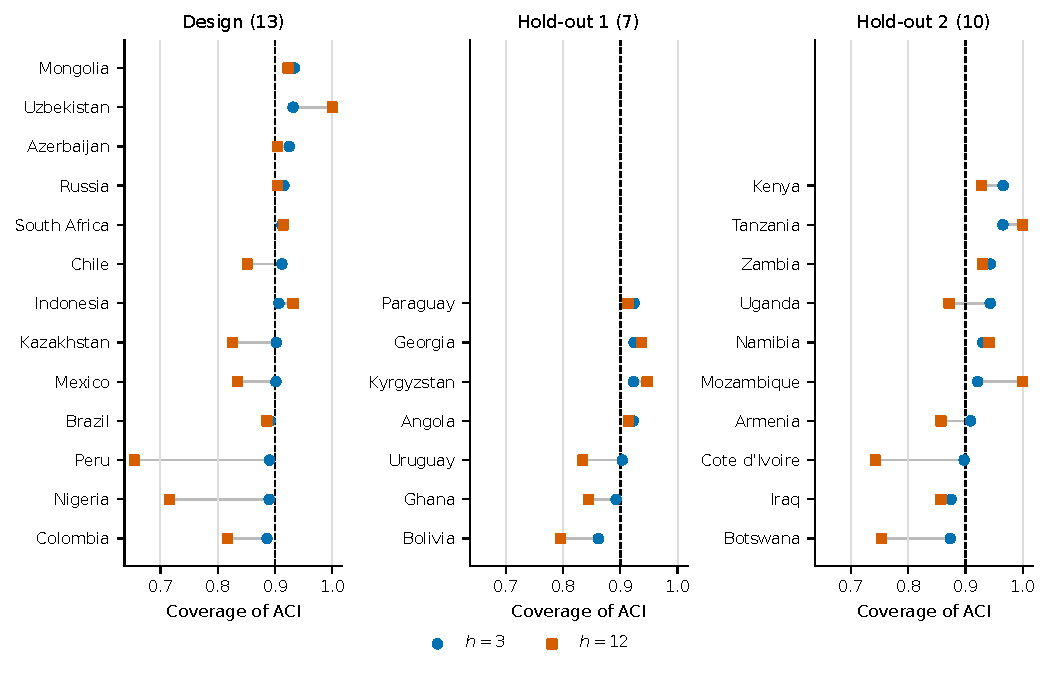
\includegraphics[width=\linewidth]{figures/fig_country_coverage.pdf}
\caption{Per-country empirical coverage of ACI, by panel, against the nominal level 0.90.}
\label{fig:country_cov}
\end{figure}

\subsection{Robustness analyses S1--S4}\label{sec:robust}

The analyses S1--S4 were written down after the hold-out result and before they were computed. They are secondary, use only existing intervals, and qualify R1--R5 without replacing them. The block length is $\max(h,12)$; S1 uses 500 bootstrap replicates and S2 and S3 use 2000.

\paragraph{S1, leave one country out (LightGBM, warm-up 48).} Table~\ref{tab:loo} shows the range of each contrast over removals and the number of removals that flip the sign of the full-sample estimate. The advantage of ACI over a calibration done once does not depend on any single country. The point estimate of ACI against rolling is negative for almost every removal, but its interval includes zero in the primary run, so ``not shown'' stands. The DRACP minus ACI estimates sit at zero and change sign when one or two countries are removed.

\begin{table}[t]
\centering
\caption{S1: range of the contrast over leave-one-country-out removals (pp of CE) and number of sign flips of the full-sample estimate.}
\label{tab:loo}
\small
\begin{tabular}{@{}lll@{}}
\toprule
Contrast, horizon & Exploratory (13 countries) & First hold-out (7 countries) \\
\midrule
ACI $-$ split, $h=3$ & $-5.1$ to $-4.2$, 0 flips & $-4.1$ to $-2.2$, 0 flips \\
ACI $-$ split, $h=6$ & $-4.1$ to $-2.5$, 0 flips & $-3.5$ to $-2.1$, 0 flips \\
ACI $-$ rolling, $h=3$ & $-2.5$ to $-1.8$, 0 flips & $-2.2$ to $-1.0$, 0 flips \\
ACI $-$ rolling, $h=6$ & $-1.7$ to $-1.3$, 0 flips & $-1.3$ to $+0.1$, 1 of 7 flips \\
DRACP $-$ ACI, $h=3$ & $0.0$ to $+0.4$, 0 flips & $-0.4$ to $-0.1$, 0 flips \\
DRACP $-$ ACI, $h=6$ & $-0.5$ to $+0.1$, 2 of 13 flips & $-0.7$ to $+0.1$, 1 of 7 flips \\
\bottomrule
\end{tabular}
\end{table}

\subsection{Width, interval score and the question of narrower intervals}\label{sec:width}

Three statistics must be kept apart when the question is whether adaptive intervals are narrower, and they do not give the same answer (Table~\ref{tab:width} and Figure~\ref{fig:width_winkler}).

\begin{table}[t]
\centering
\caption{Calibration error / Winkler ratio / median width ratio relative to rolling conformal, by panel, interval method and horizon (LightGBM, warm-up 48; a ratio below 1 is better than rolling).}
\label{tab:width}
\small
\fittable{\begin{tabular}{lcccc}
\toprule
Method & $h{=}1$ & $h{=}3$ & $h{=}6$ & $h{=}12$ \\
\midrule
\multicolumn{5}{l}{\emph{Design (13), warm-up 48}} \\
ACI & 0.013 / 0.99 / 0.91 & 0.014 / 1.06 / 0.93 & 0.035 / 1.21 / 1.11 & 0.069 / 1.00 / 1.03 \\
DRACP & 0.016 / 1.07 / 0.95 & 0.016 / 1.16 / 0.95 & 0.033 / 1.21 / 1.09 & 0.074 / 1.38 / 1.69 \\
FACI & 0.014 / 1.00 / 0.95 & 0.018 / 1.05 / 0.94 & 0.041 / 1.06 / 0.88 & 0.101 / 0.96 / 0.91 \\
Conformal PID & 0.030 / 1.00 / 0.96 & 0.033 / 1.02 / 0.98 & 0.059 / 1.02 / 0.94 & 0.105 / 1.01 / 1.01 \\
Rolling & 0.038 / 1.00 / 1.00 & 0.036 / 1.00 / 1.00 & 0.050 / 1.00 / 1.00 & 0.091 / 1.00 / 1.00 \\
Split & 0.071 / 1.08 / 1.24 & 0.060 / 1.11 / 1.29 & 0.069 / 1.02 / 1.13 & 0.139 / 0.93 / 0.94 \\
\midrule
\multicolumn{5}{l}{\emph{Hold-out 1 (7), warm-up 48}} \\
ACI & 0.020 / 0.95 / 0.84 & 0.020 / 0.99 / 0.90 & 0.025 / 1.05 / 0.88 & 0.048 / 1.12 / 1.09 \\
DRACP & 0.021 / 0.97 / 0.89 & 0.019 / 0.96 / 0.91 & 0.022 / 1.04 / 0.91 & 0.047 / 1.25 / 0.97 \\
FACI & 0.023 / 0.95 / 0.85 & 0.023 / 0.94 / 0.90 & 0.013 / 1.00 / 0.90 & 0.070 / 1.07 / 0.92 \\
Conformal PID & 0.024 / 0.98 / 0.95 & 0.028 / 0.97 / 0.95 & 0.021 / 1.00 / 0.94 & 0.079 / 1.05 / 0.99 \\
Rolling & 0.029 / 1.00 / 1.00 & 0.036 / 1.00 / 1.00 & 0.032 / 1.00 / 1.00 & 0.086 / 1.00 / 1.00 \\
Split & 0.056 / 1.11 / 1.34 & 0.050 / 1.07 / 1.23 & 0.053 / 1.06 / 1.27 & 0.119 / 1.02 / 1.09 \\
\bottomrule
\end{tabular}
}
\end{table}

\begin{figure}[t]
\centering
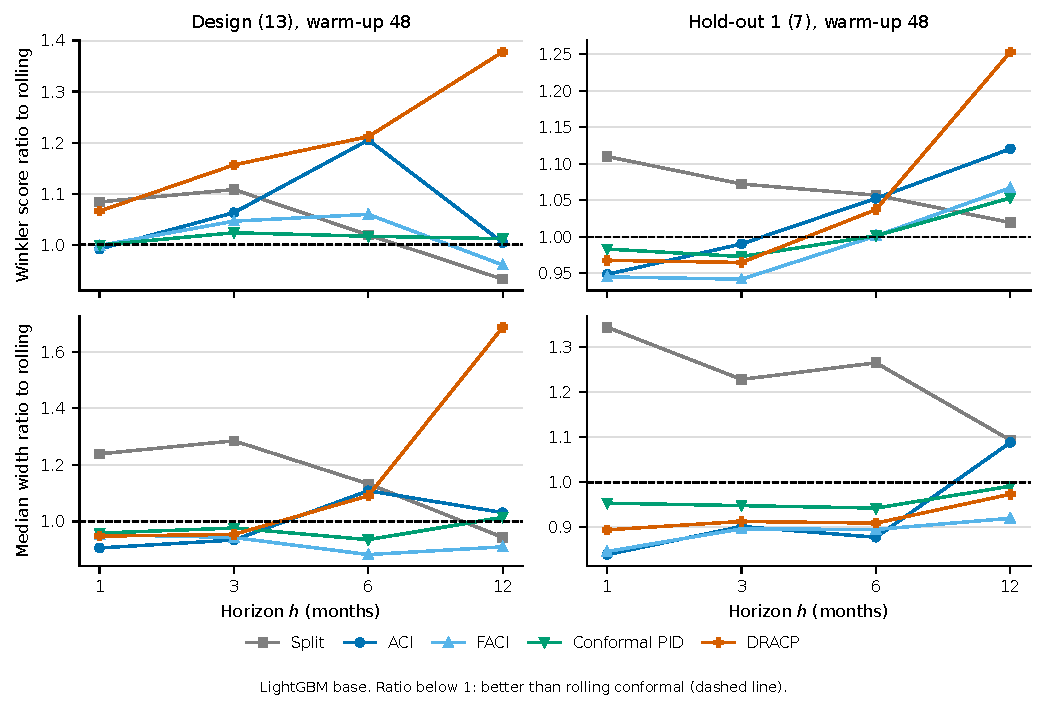
\includegraphics[width=\linewidth]{figures/fig_width_winkler.pdf}
\caption{Interval width and Winkler score of the interval methods relative to rolling conformal.}
\label{fig:width_winkler}
\end{figure}

\begin{itemize}
\item \emph{Median interval width ratio (to rolling).} At $h=1$ and $h=3$, ACI, DRACP and FACI have a median width below that of rolling in both samples: ACI 0.91 and 0.93 in the exploratory data, and 0.84 and 0.90 on the first hold-out panel.
\item \emph{Pooled mean width.} The pooled mean width of ACI at $h=3$ is larger than that of rolling in both samples: 4.28 against 3.95 in the exploratory data and 5.856 against 5.786 on the hold-out panel. This indicates heavy tails in the width of the adaptive intervals. The pooled mean width of DRACP is larger than that of ACI at $h=3$ (4.97 against 4.28) and at $h=12$ (24.3 against 15.5) in the exploratory data.
\item \emph{Winkler score.} The Winkler ratio to rolling for ACI, DRACP and FACI at $h=1$ and $h=3$ is 0.94 to 0.99 on the hold-out panel and 0.99 to 1.16 in the exploratory data (ACI 1.06 and DRACP 1.16 at $h=3$). In the exploratory data ACI's Winkler score at $h=3$ was 6.3 percent higher than rolling's (95\% interval \ci{0.3}{19.4}, unadjusted $p=0.15$). At $h=6$ and $h=12$ the Winkler ratio of ACI and DRACP is above 1 in most cells of both samples (up to 1.38).
\end{itemize}
The adaptive methods have a lower median width at short horizons, but the pooled mean width and the interval score do not show a consistent gain. No efficiency advantage is established; at long horizons the better calibration is paid for with width or interval score.

\subsection{Second hold-out panel (extension)}\label{sec:panel2}

The second hold-out panel has 10 countries with 198 months of CPI from 2010-01. At warm-up 48 there are 89 pooled calendar months at $h=3$ and 83 at $h=6$; at warm-up 96 there are 41 and 35. Four base models are used: LightGBM, ARIMA, naive B and Chronos. The Holm family has four tests per base model. Warm-up 48 is the primary run; warm-up 96 is a sensitivity run and is not promoted.

Table~\ref{tab:ce_ho2} gives the calibration error at warm-up 48. At $h=3$ and $h=6$ ACI has 0.033 and 0.045 (LightGBM), 0.034 and 0.052 (ARIMA), 0.049 and 0.052 (naive B) and 0.034 and 0.050 (Chronos); DRACP has 0.023 and 0.032, 0.019 and 0.034, 0.037 and 0.034, and 0.030 and 0.038; rolling has 0.070 and 0.080, 0.066 and 0.084, 0.090 and 0.087, and 0.067 and 0.075; split has 0.104 and 0.125, 0.098 and 0.111, 0.122 and 0.105, and 0.109 and 0.107; the native ARIMA intervals have 0.058 and 0.084. For comparison, on the first hold-out panel the calibration error of the rolling window at $h=3$ and $h=6$ is 0.036 and 0.032, against 0.066 to 0.090 and 0.075 to 0.087 here. This is a descriptive observation, and its relation to the results below was not tested.

\begin{table}[t]
\centering
\caption{Calibration error by interval method, horizon and base model, second hold-out panel (10 countries, warm-up 48).}
\label{tab:ce_ho2}
\small
\fittable{\begin{tabular}{llrrrr}
\toprule
Base model & Interval & $h{=}1$ & $h{=}3$ & $h{=}6$ & $h{=}12$ \\
\midrule
LightGBM & Split & 0.084 & 0.104 & 0.125 & 0.154 \\
 & Rolling & 0.050 & 0.070 & 0.080 & 0.089 \\
 & ACI & 0.032 & 0.033 & 0.045 & 0.072 \\
 & FACI & 0.024 & 0.027 & 0.042 & 0.079 \\
 & Conformal PID & 0.043 & 0.051 & 0.070 & 0.103 \\
 & DRACP & 0.023 & 0.023 & 0.032 & 0.078 \\
\midrule
ARIMA & Split & 0.086 & 0.098 & 0.111 & 0.136 \\
 & Rolling & 0.053 & 0.066 & 0.084 & 0.089 \\
 & ACI & 0.026 & 0.034 & 0.052 & 0.074 \\
 & FACI & 0.033 & 0.023 & 0.035 & 0.075 \\
 & Conformal PID & 0.037 & 0.047 & 0.073 & 0.105 \\
 & DRACP & 0.017 & 0.019 & 0.034 & 0.071 \\
 & Native & 0.052 & 0.058 & 0.084 & 0.132 \\
\midrule
Naive B & Split & 0.079 & 0.122 & 0.105 & 0.188 \\
 & Rolling & 0.057 & 0.090 & 0.087 & 0.110 \\
 & ACI & 0.023 & 0.049 & 0.052 & 0.089 \\
 & FACI & 0.024 & 0.049 & 0.055 & 0.082 \\
 & Conformal PID & 0.054 & 0.073 & 0.074 & 0.122 \\
 & DRACP & 0.020 & 0.037 & 0.034 & 0.087 \\
\midrule
Chronos & Split & 0.078 & 0.109 & 0.107 & 0.111 \\
 & Rolling & 0.048 & 0.067 & 0.075 & 0.078 \\
 & ACI & 0.028 & 0.034 & 0.050 & 0.062 \\
 & FACI & 0.017 & 0.031 & 0.041 & 0.088 \\
 & Conformal PID & 0.040 & 0.052 & 0.073 & 0.105 \\
 & DRACP & 0.021 & 0.030 & 0.038 & 0.082 \\
\bottomrule
\end{tabular}
}
\end{table}

Table~\ref{tab:panel2primary} gives the primary contrasts for each base model.

\begin{table}[t]
\centering
\caption{Primary contrasts, second hold-out panel, warm-up 48: $T$ in pp of CE, 95\% bootstrap interval, and Holm $p$ over the four primary tests of the base model.}
\label{tab:panel2primary}
\small
\resizebox{\linewidth}{!}{%
\begin{tabular}{@{}lllll@{}}
\toprule
Base model & ACI $-$ rolling, $h=3$ & ACI $-$ rolling, $h=6$ & DRACP $-$ ACI, $h=3$ & DRACP $-$ ACI, $h=6$ \\
\midrule
LightGBM & $-3.7$ \ci{-5.1}{-0.7}; 0.008 & $-3.5$ \ci{-4.9}{+0.5}; 0.159 & $-1.0$ \ci{-2.0}{+0.9}; 0.321 & $-1.3$ \ci{-2.7}{+2.0}; 0.337 \\
ARIMA & $-3.2$ \ci{-3.6}{-1.1}; 0.004 & $-3.1$ \ci{-3.9}{-0.5}; 0.030 & $-1.5$ \ci{-2.4}{+0.8}; 0.199 & $-1.8$ \ci{-3.4}{+0.7}; 0.199 \\
Naive B & $-4.1$ \ci{-4.9}{-1.5}; 0.004 & $-3.4$ \ci{-4.7}{-0.4}; 0.039 & $-1.2$ \ci{-2.3}{+0.9}; 0.422 & $-1.8$ \ci{-3.3}{+2.5}; 0.422 \\
Chronos & $-3.3$ \ci{-4.0}{-0.3}; 0.036 & $-2.5$ \ci{-3.6}{+0.1}; 0.088 & $-0.5$ \ci{-1.8}{+1.3}; 0.454 & $-1.2$ \ci{-2.2}{+1.3}; 0.443 \\
\bottomrule
\end{tabular}}
\end{table}

ACI minus split (secondary, unadjusted $p$, at $h=3$ and $h=6$) is $-7.0$ and $-8.0$~pp for LightGBM (0.0005, 0.0005), $-6.4$ and $-5.8$ for ARIMA (0.0005, 0.001), $-7.3$ and $-5.3$ for naive B (0.001, 0.0045) and $-7.4$ and $-5.7$ for Chronos (0.0005, 0.0005). ACI with ARIMA has a lower CE than the native ARIMA intervals (0.034 against 0.058 at $h=3$ and 0.052 against 0.084 at $h=6$); the contrast with its interval is not reported for this panel. The outcomes of the rules on this panel are as follows.

\paragraph{R1 (ACI better calibrated than split).} At warm-up 48 R1 is met for all four base models at both horizons (unadjusted $p$ at most 0.0045), by $-5.3$ to $-8.0$~pp of CE. At warm-up 96 it is not met: LightGBM (0.048) and naive B (0.032) at $h=3$ have unadjusted $p$ below 0.05, all other cells are above 0.05, and with Holm over the two horizons none is below 0.05 (0.096 and 0.064). The direction replicates, and the registered threshold is met on the second panel at warm-up 48 whereas on the first hold-out panel it was met only at warm-up 96.

\paragraph{R2 (ACI improves on rolling): the result differs from the earlier panels.} At warm-up 48 R2 is met at $h=3$ for LightGBM, ARIMA and naive B (Holm 0.008, 0.004, 0.004) and at $h=6$ for ARIMA and naive B (0.030, 0.039). For Chronos at $h=3$ the Holm $p$ is 0.036 but the minimum detectable difference is undefined, so under E5 that cell is inconclusive and is not counted as met; Chronos at $h=6$ and LightGBM at $h=6$ are not met (0.088, 0.159). On the design panel and on the first hold-out panel it was not shown, and the MDE is undefined there (inconclusive). The earlier 20 countries were re-run from 2010-01 as a secondary analysis, and R2 is not significant there: the Holm $p$-values of ACI minus rolling are 0.22 to 1.0, with the MDE undefined in every cell, so these results are inconclusive under E5 and not evidence of no effect. The results are placed side by side in Table~\ref{tab:r2panels} and are not pooled.

\begin{table}[t]
\centering
\caption{R2 across panels, warm-up 48: ACI minus rolling (pp of CE) and Holm $p$ over the four tests of the run.}
\label{tab:r2panels}
\small
\resizebox{\linewidth}{!}{%
\begin{tabular}{@{}llllp{0.34\linewidth}@{}}
\toprule
Panel and run & Base model & $h=3$ & $h=6$ & Outcome \\
\midrule
Design (13), from 2000 & LightGBM & $-2.2$; 0.090 & $-1.5$; 0.078 & Not shown (MDE undefined, inconclusive) \\
First hold-out (7), from 2000 & LightGBM & $-1.6$; 0.35 & $-0.7$; 1.0 & Not shown (MDE undefined, inconclusive) \\
Design (13), re-run from 2010 & LightGBM & $-2.1$; 0.216 & $-2.0$; 0.216 & Not met; MDE undefined in every cell: inconclusive under E5 \\
Design (13), re-run from 2010 & Chronos & $-1.9$; 0.363 & $-2.0$; 0.358 & Not met; MDE undefined in every cell: inconclusive under E5 \\
First hold-out (7), re-run from 2010 & LightGBM & $-2.4$; 0.496 & $-4.7$; 0.390 & Not met; MDE undefined in every cell: inconclusive under E5 \\
First hold-out (7), re-run from 2010 & Chronos & $-1.3$; 1.000 & $-2.0$; 0.962 & Not met; MDE undefined in every cell: inconclusive under E5 \\
Second hold-out (10), from 2010 & LightGBM & $-3.7$; 0.008 & $-3.5$; 0.159 & Met at $h=3$ \\
Second hold-out (10), from 2010 & ARIMA & $-3.2$; 0.004 & $-3.1$; 0.030 & Met at both \\
Second hold-out (10), from 2010 & Naive B & $-4.1$; 0.004 & $-3.4$; 0.039 & Met at both \\
Second hold-out (10), from 2010 & Chronos & $-3.3$; 0.036 (MDE undefined: inconclusive under E5) & $-2.5$; 0.088 & Inconclusive at $h=3$; not met at $h=6$ \\
\bottomrule
\end{tabular}}
\end{table}

Three things should be read together. First, the point estimates are negative in every row of Table~\ref{tab:r2panels}. On the second panel they ($-2.5$ to $-4.1$~pp) are generally larger than on the earlier panels ($-0.7$ to $-2.4$~pp), with one exception, LightGBM on the re-run first hold-out panel at $h=6$ ($-4.7$~pp, Holm $p=0.390$, 95\% interval \ci{-9.6}{+0.5}); so the direction does not differ between panels, but its size and its distance from the registered threshold do. Second, the conclusion that ``ACI improves on a rolling window'' is reached under the registered rule on one panel and not on the other two. The data do not say why. Candidate explanations are a shorter series (198 months from 2010), lower-income and more volatile economies, a larger share of the 198 months taken by the warm-up, and a rolling window with a larger calibration error here; none of them was tested, and none is claimed. Third, the four base models are evaluated on the same 10 countries and the same months, so the three ``met'' cells at $h=3$ are not three independent confirmations, and the Holm correction does not extend across base models. We do not average the panels into one statement and we do not select the panel on which the rule is met.

\paragraph{Warm-up 96 on the second panel shows nothing.} After a warm-up of 96 the panel has 41 pooled months at $h=3$ and 35 at $h=6$. ACI minus rolling is $-1.0$ to $-3.3$~pp at $h=3$ (Holm $p$ 0.147 to 1.0). At $h=6$ it is $+0.2$~pp (LightGBM), $+1.1$~pp (Chronos), $-0.5$~pp (ARIMA) and $-0.6$~pp (naive B), with Holm $p$ of 0.59 or more. The minimum detectable difference is undefined for every contrast. The run is a sensitivity run, it neither confirms nor contradicts the primary run, and it is not promoted.

\paragraph{R3 stays inconclusive.} At warm-up 48 DRACP has a lower CE than ACI in every cell, by 0.5 to 1.8~pp, and no difference has Holm $p$ below 0.05 (0.199 to 0.454). Equivalence within 2~pp holds only for Chronos at $h=3$ (TOST $p=0.0385$) and is not shown in the other seven cells ($p$ 0.15 to 0.76). At warm-up 96 equivalence holds for LightGBM and naive B at $h=3$ ($p=0.0375$ and 0.013) and not in the other six cells, and DRACP is better than ACI only at $h=6$ for naive B ($-2.3$~pp, Holm $p=0.002$). R3 requires the same verdict at both warm-ups, so it is not met. Under E5 every DRACP minus ACI contrast at warm-up 48 has an undefined minimum detectable difference and is inconclusive whatever its $p$-value, including the equivalence of Chronos at $h=3$. The small and consistent tendency of DRACP towards a lower CE at warm-up 48 is a descriptive observation and not a result.

\paragraph{E5, power.} At warm-up 48 the minimum detectable difference for ACI minus rolling is 3.2~pp ($h=3$) and 6.1~pp ($h=6$) for LightGBM, 3.2 and 3.5~pp for ARIMA, 1.2 and 3.5~pp for naive B, and 6.6~pp for Chronos at $h=6$; it is undefined for Chronos at $h=3$, so that cell is not conclusive under the rule even though the Holm $p$ is 0.036. Where R2 is not met (LightGBM and Chronos at $h=6$) the minimum detectable difference of 6.1 and 6.6~pp is larger than the estimates, so ``not met'' there is not evidence that the effect is absent.

\paragraph{E2, dependence on the base model.} On this panel the direction and the size of the contrasts are alike for the four base models (Tables~\ref{tab:ce_ho2} and~\ref{tab:panel2primary}). The conclusions about R1 and R3 do not depend on the base model; the conclusion about R2 at $h=6$ does (met for ARIMA and naive B, not for LightGBM and Chronos), and at $h=3$ Chronos is inconclusive under E5 while LightGBM, ARIMA and naive B are met. On the earlier 20 countries re-run from 2010-01 the effect is weaker: ACI minus rolling is $-1.3$ to $-4.7$~pp with Holm $p$ 0.22 to 1.0, and ACI minus split is $-3.5$ to $-9.4$~pp with unadjusted $p$ between 0.002 and 0.045. R4 (delayed feedback) was not part of the extension, and no instant-feedback run was made on the second panel.

\begin{figure}[t]
\centering
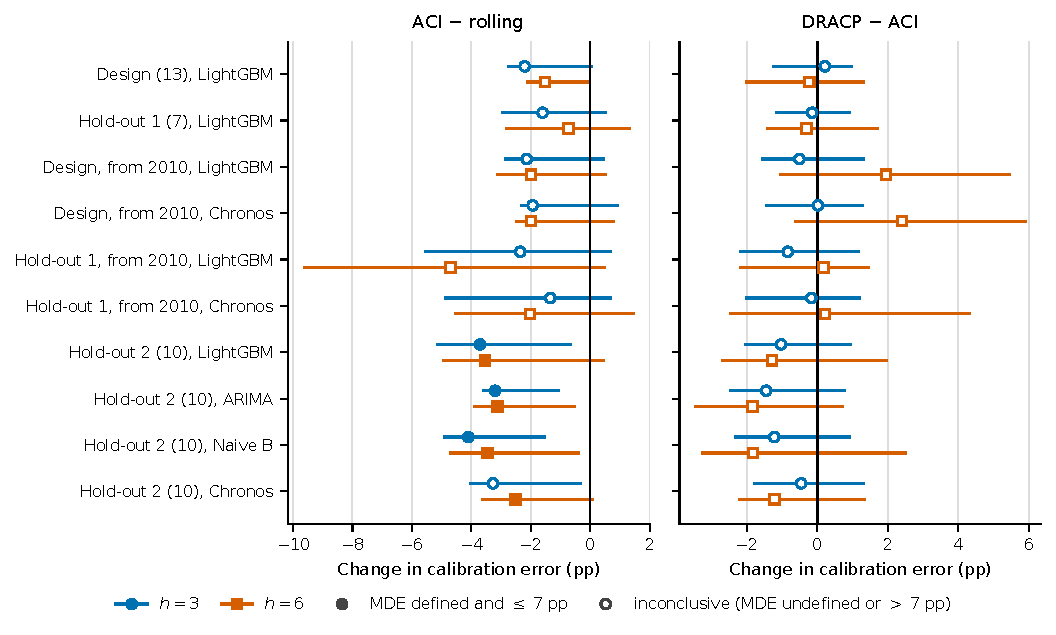
\includegraphics[width=\linewidth]{figures/fig_contrasts_forest.pdf}
\caption{Forest plot of the change in calibration error (pp) for ACI minus rolling and DRACP minus ACI, with 95\% block-bootstrap intervals. Contrasts with an undefined minimum detectable difference are inconclusive under rule E5 regardless of the interval.}
\label{fig:forest}
\end{figure}

Figure~\ref{fig:forest} shows the contrasts side by side. The figure is a display of the same estimates as in Tables~\ref{tab:contrasts},~\ref{tab:panel2primary} and~\ref{tab:r2panels}; it does not pool the panels.

\subsection{Ablation study}\label{sec:ablation}

The ablations vary one design choice at a time: the base model, the warm-up, the feedback delay, and the reference interval (native against conformal). A fifth subsection reports the point accuracy of Chronos.

\subsubsection{Base model}\label{sec:basemodel}

The contrasts were recomputed with ARIMA and naive B as base models of the conformal methods on the design and first hold-out panels (S2, Appendix Table~\ref{tab:s2full}), and Table~\ref{tab:ablation_base} gives the same ablation on the second hold-out panel with four base models. ACI minus split is negative for all three base models in both samples; for naive B at $h=6$ on the first hold-out panel it is $-10.6$~pp. All DRACP minus ACI equivalence tests at warm-up 48 say ``equivalent'' within 2~pp, except naive B at $h=6$ on the hold-out panel ($p=0.0515$); at warm-up 96 on the hold-out panel most are ``not shown''. The direction ``ACI better than rolling'' holds for every base model and both samples, but the unadjusted $p$-values range from 0.016 to 0.48, and none survives the correction of the pre-specified family. For example, at $h=3$ on the hold-out panel ACI minus rolling is $-1.6$~pp for LightGBM ($p=0.087$), $-3.0$~pp for ARIMA ($p=0.030$) and $-0.9$~pp for naive B ($p=0.22$); at $h=6$ it is $-0.7$ ($p=0.48$), $-1.6$ ($p=0.21$) and $-3.2$~pp ($p=0.053$). ARIMA and naive B give similar ACI coverage at $h=6$ in the exploratory data (0.895 and 0.908). On the second hold-out panel the base-model dependence is described in Section~\ref{sec:panel2}.

\begin{table}[t]
\centering
\caption{Ablation over the base model on the second hold-out panel (warm-up 48): relative mean absolute error (naive B $=1$, all target months including flagged months), calibration error of ACI and of rolling, and ACI minus rolling in pp of CE with Holm $p$.}
\label{tab:ablation_base}
\small
\fittable{\begin{tabular}{lrrrrrrrr}
\toprule
& \multicolumn{2}{c}{Rel. MAE} & \multicolumn{2}{c}{CE, ACI} & \multicolumn{2}{c}{CE, rolling} & \multicolumn{2}{c}{ACI $-$ rolling, pp (Holm $p$)} \\
\cmidrule(lr){2-3}\cmidrule(lr){4-5}\cmidrule(lr){6-7}\cmidrule(lr){8-9}
Base model & $h{=}3$ & $h{=}6$ & $h{=}3$ & $h{=}6$ & $h{=}3$ & $h{=}6$ & $h{=}3$ & $h{=}6$ \\
\midrule
Naive B & 1.000 & 1.000 & 0.049 & 0.052 & 0.090 & 0.087 & $-$4.1 (0.004) & $-$3.4 (0.039) \\
ARIMA & 0.602 & 0.570 & 0.034 & 0.052 & 0.066 & 0.084 & $-$3.2 (0.004) & $-$3.1 (0.030) \\
LightGBM & 0.619 & 0.593 & 0.033 & 0.045 & 0.070 & 0.080 & $-$3.7 (0.008) & $-$3.5 (0.159) \\
Chronos & 0.586 & 0.581 & 0.034 & 0.050 & 0.067 & 0.075 & $-$3.3 (0.036) & $-$2.5 (0.088) \\
\bottomrule
\end{tabular}
}
\end{table}

\subsubsection{Warm-up: 48 against 96}\label{sec:warmup}

Warm-up 96 is a sensitivity run applied to all methods; it is not promoted to the primary configuration. Table~\ref{tab:ablation_warmup} and Figure~\ref{fig:warmup} compare the two. On the first hold-out panel ACI minus split moves from $-3.0$ and $-2.8$~pp at warm-up 48 to $-4.1$ and $-5.9$~pp at warm-up 96, and this change is what turns R1 from not met to met; ACI minus rolling is $-1.6$ and $-0.7$~pp at 48 and $-1.5$ and $-1.1$~pp at 96, with Holm $p$ 0.35 and 1.0 against 0.59 and 0.99. Equivalence of DRACP and ACI is shown at warm-up 48 and not at 96 (Section~\ref{sec:holdout}). The 96-month warm-up removes target months, leaving 157 and 151 pooled months at $h=3$ and $h=6$ against 205 and 199, so the sample for the comparison is also smaller. On the second hold-out panel the warm-up of 96 leaves 41 and 35 pooled months and shows nothing (Section~\ref{sec:panel2}). The comparison between warm-ups is a sensitivity analysis and does not select a configuration.

\begin{table}[t]
\centering
\caption{Ablation over the warm-up size: calibration error of ACI and rolling, ACI minus rolling and Holm $p$ at warm-up 48 (primary) and 96 (sensitivity, not promoted), by panel.}
\label{tab:ablation_warmup}
\small
\fittable{\begin{tabular}{llcrrrrrrrr}
\toprule
\multicolumn{3}{c}{} & \multicolumn{2}{c}{CE, ACI} & \multicolumn{2}{c}{CE, rolling} & \multicolumn{2}{c}{ACI $-$ rolling (pp)} & \multicolumn{2}{c}{Holm $p$} \\
\cmidrule(lr){4-5}\cmidrule(lr){6-7}\cmidrule(lr){8-9}\cmidrule(lr){10-11}
Panel & Base & $h$ & 48 & 96 & 48 & 96 & 48 & 96 & 48 & 96 \\
\midrule
Design (13) & LightGBM & 3 & 0.014 & 0.022 & 0.036 & 0.035 & $-$2.2 & $-$1.3 & 0.090 & 0.132 \\
 &  & 6 & 0.035 & 0.039 & 0.050 & 0.054 & $-$1.5 & $-$1.5 & 0.078 & 0.132 \\
\midrule
Hold-out 1 (7) & LightGBM & 3 & 0.020 & 0.027 & 0.036 & 0.042 & $-$1.6 & $-$1.5 & 0.350 & 0.592 \\
 &  & 6 & 0.025 & 0.030 & 0.032 & 0.041 & $-$0.7 & $-$1.1 & 1.000 & 0.990 \\
\midrule
Hold-out 2 (10) & LightGBM & 3 & 0.033 & 0.045 & 0.070 & 0.058 & $-$3.7 & $-$1.3 & 0.008 & 0.278 \\
 &  & 6 & 0.045 & 0.069 & 0.080 & 0.067 & $-$3.5 & +0.2 & 0.159 & 1.000 \\
\midrule
Hold-out 2 (10) & ARIMA & 3 & 0.034 & 0.043 & 0.066 & 0.053 & $-$3.2 & $-$1.0 & 0.004 & 0.340 \\
 &  & 6 & 0.052 & 0.081 & 0.084 & 0.086 & $-$3.1 & $-$0.5 & 0.030 & 0.682 \\
\midrule
Hold-out 2 (10) & Naive B & 3 & 0.049 & 0.050 & 0.090 & 0.083 & $-$4.1 & $-$3.3 & 0.004 & 0.147 \\
 &  & 6 & 0.052 & 0.071 & 0.087 & 0.077 & $-$3.4 & $-$0.6 & 0.039 & 0.593 \\
\midrule
Hold-out 2 (10) & Chronos & 3 & 0.034 & 0.048 & 0.067 & 0.063 & $-$3.3 & $-$1.5 & 0.036 & 1.000 \\
 &  & 6 & 0.050 & 0.084 & 0.075 & 0.073 & $-$2.5 & +1.1 & 0.088 & 1.000 \\
\bottomrule
\end{tabular}
}
\end{table}

\begin{figure}[t]
\centering
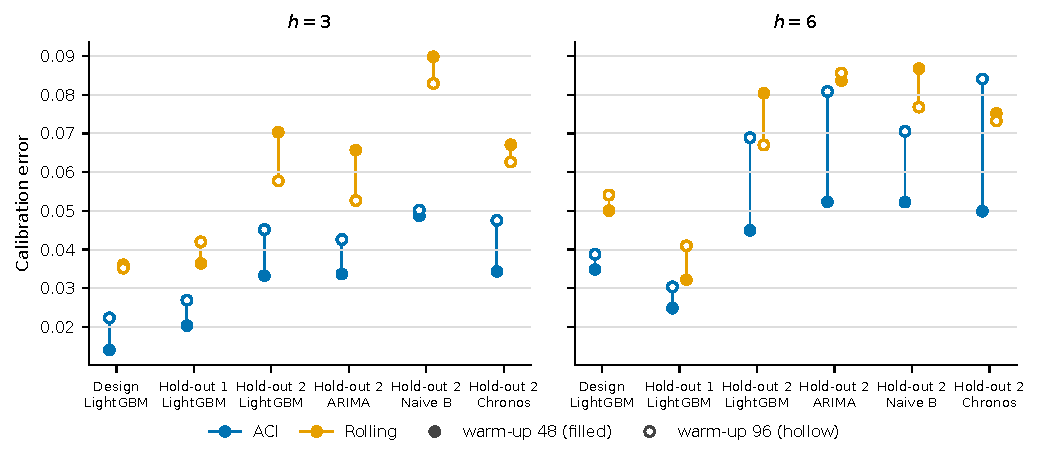
\includegraphics[width=\linewidth]{figures/fig_warmup_sensitivity.pdf}
\caption{Sensitivity of the contrasts to the warm-up size (48 against 96 residuals). Warm-up 96 is a sensitivity run and is not promoted to the primary result.}
\label{fig:warmup}
\end{figure}

\subsubsection{Feedback delay}\label{sec:feedback}

At $h=12$ pooled coverage is below nominal for every method (0.83 to 0.88 on the first hold-out panel, 0.82 to 0.87 in the exploratory data), with the qualification on the bootstrap intervals given in Section~\ref{sec:explor}. To examine the role of delayed feedback, the diagnostic run releases each outcome at origin $+1$ instead of origin $+12$. Table~\ref{tab:feedback} gives coverage with instant feedback minus coverage with delayed feedback, with a paired block-bootstrap 95 percent interval over the same (unit, origin) cells. For ACI the change is $+4.1$~pp (\ci{1.4}{7.8}) in the exploratory data (1738 cells) and $+2.4$~pp (\ci{-0.1}{4.8}) on the hold-out panel (1009 cells); for DRACP $+4.3$ (\ci{1.4}{7.5}) and $+3.9$~pp (\ci{1.6}{6.5}); for FACI $+8.3$ (\ci{4.3}{13.6}) and $+6.4$~pp (\ci{2.5}{9.6}); for conformal PID $+5.1$ and $+5.3$~pp; for rolling $+1.3$~pp in both; split conformal does not use feedback, so its difference is zero by construction.

\begin{table}[t]
\centering
\caption{Ablation over the feedback delay (S3): coverage at $h=12$ with delayed and with instant feedback, and the difference in pp with a 95\% paired block-bootstrap interval.}
\label{tab:feedback}
\small
\fittable{\begin{tabular}{lrrcrrc}
\toprule
& \multicolumn{3}{c}{Design (13), 1738 cells} & \multicolumn{3}{c}{Hold-out 1 (7), 1009 cells} \\
\cmidrule(lr){2-4}\cmidrule(lr){5-7}
Method & Delayed & Instant & Diff. (pp) [95\% CI] & Delayed & Instant & Diff. (pp) [95\% CI] \\
\midrule
Split & 0.864 & 0.864 & +0.0 [+0.0, +0.0] & 0.861 & 0.861 & +0.0 [+0.0, +0.0] \\
Rolling & 0.869 & 0.882 & +1.3 [+0.2, +3.1] & 0.872 & 0.885 & +1.3 [+0.1, +1.7] \\
ACI & 0.864 & 0.905 & +4.1 [+1.4, +7.8] & 0.884 & 0.908 & +2.4 [$-$0.1, +4.8] \\
FACI & 0.825 & 0.907 & +8.3 [+4.3, +13.6] & 0.835 & 0.900 & +6.4 [+2.5, +9.6] \\
Conformal PID & 0.837 & 0.888 & +5.1 [+2.0, +9.0] & 0.833 & 0.886 & +5.3 [+2.5, +7.9] \\
DRACP & 0.863 & 0.906 & +4.3 [+1.4, +7.5] & 0.865 & 0.904 & +3.9 [+1.6, +6.4] \\
\bottomrule
\end{tabular}
}
\end{table}

On the hold-out panel ACI coverage is 0.884 with delayed feedback and 0.908 with instant feedback. R4 as registered (ACI at least $+3$~pp) is not met: the result is $+2.4$~pp. The interval \ci{-0.1}{4.8} is compatible with no effect and with an effect of about 5~pp. For FACI and DRACP the effect is positive in both samples. The statement supported is that feedback delay accounts for part of the shortfall at $h=12$, with a size that depends on the method and the sample. It is not shown that delay is, or is not, the main cause. The diagnostic is not a valid forecasting setup and is not a primary result.

\subsubsection{Native intervals against conformal calibration}\label{sec:native}

The analysis S7 compares conformal calibration with the native (parametric) intervals of ARIMA (Gaussian) and ETS (simulated). It is post hoc (seventh protocol entry), secondary and carries no multiplicity correction; the $p$-values are unadjusted and descriptive. ETS has no conformal version in the engine, so for ETS the native calibration error is reported without a contrast. Table~\ref{tab:native} gives the mean over countries of the calibration error. In the exploratory data the native ARIMA intervals have a CE of 0.047, 0.066, 0.089 and 0.137 at $h=1,3,6,12$ against 0.010, 0.015, 0.026 and 0.079 for ARIMA with ACI, and native ETS has 0.044, 0.051, 0.064 and 0.116. On the first hold-out panel the corresponding numbers are 0.053, 0.058, 0.062 and 0.073 (native ARIMA), 0.014, 0.013, 0.024 and 0.040 (ARIMA with ACI) and 0.056, 0.035, 0.048 and 0.053 (native ETS).

\begin{table}[t]
\centering
\caption{Ablation over the reference interval (S7, post hoc): calibration error of native ARIMA and ETS intervals and of ARIMA with ACI, and the contrast ACI minus native (pp of CE, 95\% interval, unadjusted $p$).}
\label{tab:native}
\small
\fittable{\begin{tabular}{lcrrrcr}
\toprule
Panel & $h$ & ARIMA native & ARIMA + ACI & ETS native & ACI $-$ native, pp [95\% CI] & $p$ \\
\midrule
Design (13) & 1 & 0.047 & 0.010 & 0.044 & $-$3.7 [$-$4.6, $-$0.6] & 0.004 \\
 & 3 & 0.066 & 0.015 & 0.051 & $-$5.1 [$-$6.2, $-$1.0] & 0.003 \\
 & 6 & 0.089 & 0.026 & 0.064 & $-$6.4 [$-$7.7, $-$1.3] & 0.002 \\
 & 12 & 0.137 & 0.079 & 0.116 & $-$5.8 [$-$7.8, $-$1.9] & 0.003 \\
\midrule
Hold-out 1 (7) & 1 & 0.053 & 0.014 & 0.056 & $-$3.9 [$-$4.5, $-$1.3] & $<$0.001 \\
 & 3 & 0.058 & 0.013 & 0.035 & $-$4.5 [$-$4.8, $-$0.6] & 0.010 \\
 & 6 & 0.062 & 0.024 & 0.048 & $-$3.8 [$-$4.4, +1.2] & 0.082 \\
 & 12 & 0.073 & 0.040 & 0.053 & $-$3.3 [$-$4.9, +1.3] & 0.100 \\
\midrule
Hold-out 2 (10) & 1 & 0.052 & 0.026 & -- & -- & -- \\
 & 3 & 0.058 & 0.034 & -- & -- & -- \\
 & 6 & 0.084 & 0.052 & -- & -- & -- \\
 & 12 & 0.132 & 0.074 & -- & -- & -- \\
\bottomrule
\end{tabular}
}
\end{table}

The contrast ACI minus native, with ARIMA as base model, is in the exploratory data $-3.7$, $-5.1$, $-6.4$ and $-5.8$~pp at $h=1,3,6,12$ (95\% intervals \ci{-4.6}{-0.6}, \ci{-6.2}{-1.0}, \ci{-7.7}{-1.3}, \ci{-7.8}{-1.9}; unadjusted $p$ 0.004, 0.003, 0.002, 0.003) and on the first hold-out panel $-3.9$ (\ci{-4.5}{-1.3}; $p$ below 0.001), $-4.5$ (\ci{-4.8}{-0.6}; 0.010), $-3.8$ (\ci{-4.4}{+1.2}; 0.082) and $-3.3$~pp (\ci{-4.9}{+1.3}; 0.100). Conformal calibration with ACI gives a lower calibration error than the native intervals of the same ARIMA model at every horizon in both samples, by about 3 to 6~pp. On the hold-out panel the interval for the difference excludes zero at $h=1$ and $h=3$ and includes zero at $h=6$ and $h=12$. The mean coverage of the native ARIMA intervals looks acceptable on the hold-out panel (0.943, 0.930, 0.919 and 0.885 at $h=1,3,6,12$) because over-coverage in some countries offsets under-coverage in others; the calibration error shows the dispersion. The ETS native intervals have calibration errors of the same order as the ARIMA native ones in both samples. This contrast is secondary and post hoc, so the evidence against native intervals is weaker in procedure than the pre-specified contrasts, although its direction is consistent.

\subsubsection{Point accuracy of Chronos}\label{sec:chronos}

Months before 2025-01 are flagged \texttt{possibly\_seen} for Chronos, which may have met these public series in pretraining. The relative mean absolute error on the second hold-out panel over all target months, warm-up 48 (naive B $=1$; below 1 is better), is 0.737, 0.586, 0.581 and 0.934 for Chronos at $h=1,3,6,12$, against 0.779, 0.602, 0.570 and 0.880 for ARIMA and 0.817, 0.619, 0.593 and 0.943 for LightGBM. This comparison includes months on which Chronos may have an unfair advantage and is not used for any claim about Chronos; it has no intervals and no ETS, which deviates from E3 (Section~\ref{sec:extension}).

Following E4, claims about accuracy are drawn only from target months from 2025-01. These are 22 calendar months with 567 country-month cells per horizon, pooled over the 30 countries of the three panels. Table~\ref{tab:chronos_mae} gives the relative mean absolute error by horizon and model and the difference in mean absolute error (Chronos minus the other model, in pp of cumulative growth; negative favours Chronos) with a paired block-bootstrap 95\% interval (blocks of 3 months, months resampled jointly across countries); the intervals are unadjusted and descriptive. Figure~\ref{fig:chronos} displays the comparison.

\begin{table}[t]
\centering
\caption{Point accuracy of Chronos on the clean target months from 2025-01 (22 months, 30 countries): mean absolute error relative to naive B, and difference in mean absolute error with a paired block-bootstrap 95\% interval (pp; negative favours Chronos).}
\label{tab:chronos_mae}
\small
\fittable{\begin{tabular}{crrrccc}
\toprule
& \multicolumn{3}{c}{Relative MAE (naive B $=1$)} & \multicolumn{3}{c}{MAE difference, Chronos $-$ other (pp)} \\
\cmidrule(lr){2-4}\cmidrule(lr){5-7}
$h$ & Chronos & LightGBM & ARIMA & vs LightGBM & vs ARIMA & vs naive B \\
\midrule
1 & 0.774 & 0.824 & 0.854 & $-$0.023 [$-$0.047, $-$0.007] & $-$0.037 [$-$0.053, $-$0.021] & $-$0.104 [$-$0.134, $-$0.081] \\
3 & 0.699 & 0.725 & 0.773 & $-$0.031 [$-$0.078, +0.036] & $-$0.086 [$-$0.139, $-$0.031] & $-$0.350 [$-$0.519, $-$0.206] \\
6 & 0.654 & 0.694 & 0.700 & $-$0.084 [$-$0.129, $-$0.025] & $-$0.097 [$-$0.204, +0.002] & $-$0.720 [$-$0.905, $-$0.527] \\
12 & 0.895 & 0.995 & 0.905 & $-$0.245 [$-$0.465, $-$0.019] & $-$0.024 [$-$0.122, +0.139] & $-$0.256 [$-$0.449, $-$0.041] \\
\bottomrule
\end{tabular}
}
\end{table}


\begin{figure}[t]
\centering
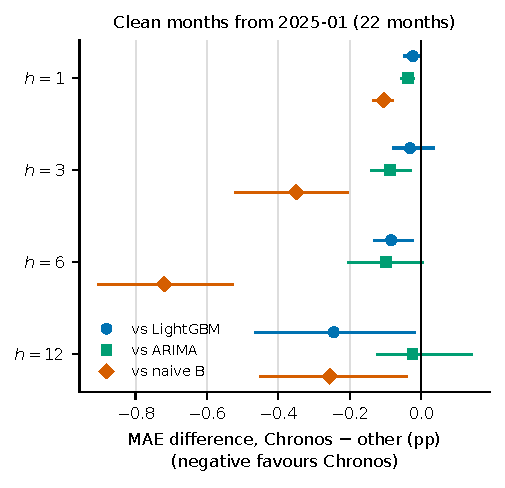
\includegraphics[width=\linewidth]{figures/fig_chronos_accuracy.pdf}
\caption{Point accuracy of Chronos relative to the other forecasters by horizon. Claims are limited to the 22 target months from 2025-01; earlier months are flagged as possibly seen in pretraining.}
\label{fig:chronos}
\end{figure}

On these clean months the relative mean absolute error of Chronos is 0.774, 0.699, 0.654 and 0.895 at $h=1,3,6,12$ (LightGBM 0.824, 0.725, 0.694, 0.995; ARIMA 0.854, 0.773, 0.700, 0.905). Against LightGBM the interval excludes zero at $h=1$, 6 and 12, and against ARIMA at $h=1$ and 3 (at $h=6$ its upper limit is $+0.002$); against naive B it excludes zero at every horizon. No interval favours LightGBM or ARIMA over Chronos. The reading is that Chronos was at least as accurate as LightGBM and ARIMA in this period and more accurate than the naive baseline. The sample is thin (22 months), the block length is short because of it, the leakage assumption (a cutoff of 2025-01) is not verified, and the results are descriptive and not a ranking of forecasters. Calibration contrasts for Chronos (Section~\ref{sec:panel2}) use all months with the flag, as specified in E4, and no calibration analysis restricted to the clean months is reported.

\subsection{Stress, post-2025-06 months and Kazakhstan}\label{sec:other}

\paragraph{Stress analysis (secondary, exploratory).} For the exploratory sample at $h=3$, coverage in the top decile of exchange-rate stress at the forecast origin is 0.849 for ACI, 0.869 for DRACP and 0.874 for split, against roughly 0.87 to 0.98 in the other deciles; at $h=6$ it is 0.864, 0.879 and 0.874. With about 200 observations per decile the standard error is roughly 2.5~pp, so the top-decile shortfall of ACI at $h=3$ is about two standard errors. The deciles in between are not monotone. The same 13 countries shaped the design, many deciles, methods and horizons were examined, and the underlying association between stress and forecast error is weak (Section~\ref{sec:shockvalid}). No stress result is reported for the hold-out panels, and no confirmatory claim about stress is made.

\paragraph{The post-2025-06 months of the 13 countries (not used).}\label{sec:confirm13} The run \texttt{confirm13} evaluates the 13 design countries on target months from 2025-07. Eleven countries contribute (Nigeria ends in 2024-12 because of the CPI break; Russia has no usable stretch after 2022-03), each with at most 16 months. With blocks of 12 months on at most 16 months the run is degenerate: confidence limits coincide with the estimate and $p$-values sit at the resampling floor. It is not used for any claim. Pooled coverage in that period is high for every method (ACI 0.904, 0.922 and 0.940 at $h=1,3,6$, from 167 unit-months), which is consistent with calmer inflation, and no conclusion is drawn.

\paragraph{Kazakhstan (post hoc, descriptive).}\label{sec:kz} The title does not name Kazakhstan because the main results contain no separate Kazakhstan analysis, but Kazakhstan was the original focus of the study, so it is reported alone. The analysis S6 is post hoc, descriptive and carries no test. Kazakhstan is one of the 13 design countries, so the numbers come from the exploratory sample and are not independent of the design. There are 137 monthly origins at $h=1$ (133, 127 and 115 at $h=3,6,12$), with target months 2014-02 to 2025-06, so the period after the August 2015 float is mixed with the preceding managed regime. The standard error of a coverage figure from about 137 correlated origins is roughly 3~pp, so only the larger gaps are clearly outside noise. ACI, DRACP and FACI stay close to 0.90 up to $h=6$ (Appendix~\ref{app:extra}), while the rolling window, conformal PID and the one-shot split calibration under-cover at short horizons (rolling 0.825 and split 0.730 at $h=1$); at $h=12$ coverage is below nominal for every method (0.713 to 0.835). The pattern is consistent with a series that changed regime in 2015, where a calibration that cannot adapt fast enough falls behind, but the data do not isolate that mechanism.

\subsection{The language-model explainer: status}

The evaluation of the explanation layer (Section~\ref{sec:platform}) has not been run on a real language model, and no result is reported. The test suite of the explanation layer has 18 tests (31 together with the 13 platform-service tests); these tests exercise the code with a deterministic fake client and are not results about a language model.

\section{Discussion}\label{sec:discussion}

\subsection{What is established and what is not}

Four statements are supported by the evidence, with the qualifications given. First, adaptive conformal intervals (ACI, FACI, conformal PID, DRACP) were better calibrated than a conformal calibration performed once on the first months and never updated. The direction is the same in the exploratory data, on the first hold-out panel at both warm-ups, for three base forecasters, and after removing any single country (Table~\ref{tab:loo}). The strength of the evidence depends on the warm-up size: the pre-specified rule R1 was met on the first hold-out panel only at warm-up 96, which is a sensitivity run, and at the primary warm-up 48 the confidence intervals of the contrast include zero (\ci{-5.4}{+0.5} at $h=3$ and \ci{-3.9}{+1.2} at $h=6$). The statement is therefore one of consistent direction, not of a pre-specified confirmation on that panel. On the second hold-out panel R1 was met at warm-up 48 for all four base models and not at warm-up 96, which adds a replication at the primary warm-up on new countries. Second, in a secondary, post hoc analysis, ACI with an ARIMA base model had a lower calibration error than the native ARIMA intervals at every horizon in both samples; on the first hold-out panel the interval includes zero at $h=6$ and $h=12$. Third, at the 12-month horizon pooled coverage is below nominal for every method on the design and first hold-out panels, and delayed feedback accounts for part of the shortfall, the size depending on the method and sample. Fourth, at short horizons ACI, DRACP and FACI have a median interval width below that of a rolling window in both samples, but the pooled mean width of ACI at $h=3$ is larger than that of rolling in both samples, and the Winkler ratio to rolling is below 1 only on the hold-out panel at $h=1$ and $h=3$ (0.95 and 0.99 for ACI, with an interval at $h=3$ that includes zero); no efficiency advantage is established.

Three statements are not established, and the first of them is split by panel. (i) Whether ACI improves on a rolling window depends on the panel. On the design panel and the first hold-out panel it was not shown (R2); the point estimates are negative, in the direction of an advantage of about 1 to 3~pp of CE, but they do not reach the pre-specified level and their MDE is undefined, so they are inconclusive. The re-run of the earlier 20 countries from 2010-01 shows the rule as not significant (Holm $p$ 0.22 to 1.0), again with the MDE undefined in every cell and so inconclusive under E5. On the second hold-out panel the rule is met at warm-up 48 at $h=3$ for LightGBM, ARIMA and naive B (Holm 0.008, 0.004, 0.004) and at $h=6$ for ARIMA and naive B (0.030, 0.039); for Chronos at $h=3$ the Holm $p$ is 0.036 but the MDE is undefined, so it is inconclusive under E5 and not counted as met, and Chronos and LightGBM at $h=6$ are not met (0.088, 0.159). The reason for the difference is not known, and candidate explanations were not tested. The panels are not pooled; the statement supported by the evidence taken together is that the result is panel dependent, and it is neither ``ACI does not improve on a rolling window'' nor ``ACI improves on a rolling window''. (ii) An advantage of DRACP over ACI was not detected, and equivalence within 2~pp was not stable across warm-up sizes (R3); on the second panel DRACP had a lower CE than ACI in every cell at warm-up 48 by 0.5 to 1.8~pp, with no difference at Holm $p$ below 0.05, and the verdict stays inconclusive. (iii) That delayed feedback explains the $h=12$ shortfall was not met at the pre-specified threshold (R4). None of these results is evidence that the effects are absent. In particular, the wording ``DRACP does not transfer'' or ``ACI and DRACP are equal'' is not allowed by the data. Two descriptive findings of the extension carry no inferential weight: Chronos used zero-shot as a base forecaster leaves the calibration conclusions unchanged, and on the 22 target months from 2025-01 its mean absolute error was at least as low as that of LightGBM and ARIMA. The language-model explainer was evaluated on one model with programmatic metrics (Section~\ref{sec:explainer}); that result is outside the main claims, and nothing general is claimed about the faithfulness of such a layer: the grounded result is a ceiling of what the metrics see, the corrected metrics are post hoc and were checked by one reader that was the model, and the ungrounded condition is a floor.

\subsection{Why null results: power, the ceiling effect and the equivalence margin}\label{sec:nulls}

Several reasons may contribute to the null outcomes, and the data do not allow us to apportion them.

\paragraph{Sample size and dependence.} The first hold-out panel has 7 countries and about 200 origin months at $h=3$. Errors of $h$-step forecasts overlap, adaptive methods have a long memory (about 50 months at step 0.02), and countries share common shocks. The block bootstrap respects this dependence at the cost of wide intervals; the 95 percent intervals of the primary contrasts are about 2 to 6~pp wide on the CE scale.

\paragraph{Ceiling effect.} The calibration error of the rolling baseline is already small on the first hold-out panel: 0.029 at $h=1$, 0.036 at $h=3$ and 0.032 at $h=6$, and ACI's is 0.020, 0.020 and 0.025. There is little room to improve. The power simulation reflects this: its alternative cannot reduce CE below zero, so the improvement it can create is bounded by the baseline CE (about 3 to 4~pp), and 80 percent power at the first Holm step was not reached up to 10~pp on the full hold-out sample. The MDE is therefore undefined for all four primary contrasts (R5). The same is true for the exploratory sample. On random 15-month windows the median MDE is 2.6 to 3.1~pp on the hold-out panel, but it is undefined in 63 to 68 percent of windows. A contrast without defined power cannot support a claim of absence of an effect, and the pre-specified R5 therefore classifies all four contrasts as inconclusive. We interpret this as a limit of the design (a small and already well-calibrated reference) and not as a finding about the methods.

\paragraph{The equivalence margin is about the size of ACI's own calibration error.} The margin of 2~pp is about the size of the calibration error of ACI itself (0.013 and 0.014 at $h=1$ and $h=3$ in the exploratory data, and 0.020 and 0.020 on the hold-out panel). A test of whether DRACP differs from ACI by less than 2~pp therefore asks whether a method with an error of about 2~pp differs from another by less than that amount, and the verdict ``equivalent'' is weak by construction. For the same reason the contrasts against ACI cannot be powered: this is a ceiling effect, and the null outcomes for ACI against rolling and for DRACP against ACI were likely before the run. The informative contrasts are those against weak references, split (CE 0.050 to 0.056 on the hold-out panel at $h=1$ to 6) and the native intervals, where there is room for a difference. The margin was fixed in advance and is not justified beyond that.

\paragraph{The ACI-against-rolling result depends on the panel.} The second hold-out panel is an honest counter-example to the null outcomes above, and it must be reported next to them. At warm-up 48 the pre-specified rule R2 is met there in part of the cells (Table~\ref{tab:r2panels}), where it was not shown on the design panel and the first hold-out panel, and it is not significant on the earlier 20 countries re-run from 2010-01, where the MDE is undefined in every cell, so those results are inconclusive and not evidence of no effect. The data do not say why. Panel differences are candidate explanations: a shorter series (198 months from 2010-01), lower-income and more volatile economies, a warm-up that takes a larger share of 198 months, and a larger calibration error of the rolling window, which leaves more room (0.066 to 0.090 at $h=3$ against 0.036 on the first hold-out panel). The last point is consistent with the ceiling argument above, because on this panel the minimum detectable difference for ACI minus rolling is defined (1.2 to 6.6~pp), but consistency is not a test, and none of these candidates was tested. Warm-up 96 on the new panel cannot arbitrate: it has 41 and 35 pooled months, an undefined minimum detectable difference and point estimates of both signs. Two reading errors are avoided. The panels are not averaged into a single estimate, because they differ in the number of countries, the length of the series, the start date and the base models, and because the pre-specified rules apply to each panel by itself. The favourable panel is not selected either: the evidence is one panel on which the rule is met in part of the cells and two on which it is not, and a correction across the four base models, which share their countries and months, was not applied. A reader who wants a recommendation for a new set of countries cannot take it from this study.

\paragraph{A true small or zero difference.} The data are also compatible with ACI and a rolling window being close to each other in this setting, and with DRACP and ACI being close, but this cannot be separated from low power with the present sample.

\paragraph{Specific to DRACP.} DRACP trains its regime and scale models on half of the warm-up (24 rows at warm-up 48), which is a small sample for these models, and its results depend on the warm-up: equivalence holds at 48 and not at 96. In the exploratory data at warm-up 96, DRACP was wider than ACI: its Winkler score was 33 percent higher at $h=3$. This does not hold on the first hold-out panel: at warm-up 96 the Winkler score of DRACP was 5.8 percent lower than that of ACI at $h=3$ (95\% interval \ci{-14.2}{+3.3}, unadjusted $p=0.18$), with a mean width of 6.11 against 6.31, and the mean width of DRACP is larger than ACI's only in the exploratory data (4.97 against 4.28 at $h=3$). The authors of DRACP state that the advantage of their method is specific to one-step-ahead forecasting and depends on the point forecaster; the present design uses multi-month cumulative targets, a different point forecaster and a different panel, and it does not test their one-step claim. Our reproduction of the one-step setting was partial and qualitative: ACI 0.874 and DRACP 0.871 in coverage over 5 countries with one seed, against 0.884 and 0.890 reported by the authors over 48 series, so the claim of being closest to nominal could not be distinguished from ACI there either. This is a limitation of the transfer comparison and not a finding about the method.

\subsection{Calibrated is not the same as useful}

A prediction interval can reach its nominal coverage with very wide intervals, and calibration error alone does not say whether the interval is informative. This is why width and the interval score are reported next to CE. The widths show the cost: in the exploratory data the pooled mean width of ACI intervals is 4.28 percentage points of cumulative growth at $h=3$ and 15.5 at $h=12$, and at long horizons the better calibration of the adaptive methods is paid for in width or interval score. At $h=12$ an interval with honest 90 percent coverage may be too wide for practical policy or business use. The study does not establish a width at which an interval becomes useful and does not compare widths with a decision-relevant threshold.

\subsection{Implications for practice}

A practitioner who produces inflation intervals for a commodity-dependent economy should not calibrate once and leave the calibration unchanged: one-shot calibration had a higher calibration error than ACI in every CE contrast reported with LightGBM, ARIMA and naive B (both samples, both warm-ups), and for Chronos in all but one cell (the second hold-out panel at warm-up 96 and $h=6$, where the difference is $+0.8$~pp and not distinguishable from zero), although the pre-specified rule R1 was met on the first hold-out panel only at the sensitivity warm-up and the confidence intervals at the primary warm-up include zero. Its coverage also varied the most across countries (the standard deviation of coverage across units at $h=12$ is 0.152 for split against 0.058 for ACI on the first hold-out panel). The native intervals of an ARIMA model had a higher calibration error than ACI on the same model in both samples, in a post hoc comparison. Updating the calibration, with a rolling window or with ACI, had a lower calibration error than calibrating once in every cell reported (a descriptive comparison for the rolling window, for which no contrast against split was tested) and is cheap to implement. Between a rolling window and ACI this study cannot recommend one on statistical grounds, because the comparison depends on the panel (not shown on two panels, met at warm-up 48 in part of the cells on a third), and it cannot recommend one on efficiency grounds either: the median width of ACI is smaller at short horizons, but the pooled mean width and the Winkler score do not show a consistent gain. At the 12-month horizon pooled coverage is below nominal for every method (0.83 to 0.88 on the first hold-out panel), and users should treat the nominal level there as an upper bound. A part of the shortfall comes from the delay with which the outcome arrives and cannot be removed in real use.

\subsection{The choice of ACI in the platform}

The platform uses ACI. ACI was chosen as an adaptive method that is better calibrated than a one-shot calibration and than native intervals, and it is simple to implement and explain. The benchmark did not show it to be better than a rolling window on the design panel and the first hold-out panel, and on the second hold-out panel it was better at warm-up 48 in part of the cells; the result depends on the panel. No efficiency advantage is claimed. The platform module is an engineering application with a simpler point forecast and is not a scientific contribution of the paper. It displays measured backtest coverage next to the nominal level so that a user can see the actual calibration.

\subsection{Scope of the hold-out and of the term ``commodity-dependent''}

The hold-out countries are independent of the design sample by country only. They share calendar months with it, including the global shocks of 2020 to 2022, so common shocks affect both samples. The methods, the contrasts and the horizons were chosen on the design countries. The agreement between the samples is therefore weaker evidence of generality than if the hold-out countries had been observed in different periods. The second hold-out panel (2010 to 2026) shares calendar months with both earlier samples in the same way, and its rules E1--E5 were written after all earlier results were known. Its agreement with the earlier samples on R1 and its disagreement on R2 are both results about new countries and not about new periods. No export-share criterion defines commodity dependence in any panel, so the phrase in the title describes the intended setting and not a tested property.

\section{Limitations}\label{sec:limitations}

The following limitations are stated in full; items 16 to 20 concern the extension, and item 21 the distinction between a calibrated and a useful interval.

\begin{enumerate}
\item \textbf{Procedural boundary.} The hold-out countries are untouched with respect to countries only, and they share calendar months with the design sample. The methods, the form of the contrasts, the horizons, the margin of 2~pp and the thresholds of 3~pp and 7~pp were chosen on the 13 design countries, and the author had seen the post-2025-06 months of these countries before the amendments. The rules R1 to R5 were written after the exploratory results at both warm-ups were known. The pre-specification is a repository commit history, kept by one author and self-attested, with all entries on 2026-11-18 or 2026-11-19, and not an external registry or an independent timestamp.
\item \textbf{Power and the ceiling effect.} The minimum detectable difference is undefined on the full first hold-out sample for all four primary contrasts. All null outcomes are therefore inconclusive and are not evidence of equality. The 2~pp equivalence margin is about the size of ACI's own calibration error, so the equivalence verdict for DRACP against ACI is weak by construction and the contrasts against ACI cannot be powered; null outcomes were likely before the run. The MDE simulation has not been reviewed independently, and it assumes that the observed hit pattern of the baseline describes the true dependence and that dependence beyond the block length is zero.
\item \textbf{Small panel.} The first hold-out panel has 7 countries; Ghana and Angola have high-inflation episodes, so pooled results can be driven by few units. S1 shows that removing one country changes the sign of ACI against rolling at $h=6$ on the hold-out panel in one case of seven.
\item \textbf{One point-forecaster family dominates the decision rules (Sections~\ref{sec:explor} and~\ref{sec:holdout}).} LightGBM is the base model for the primary family of R1--R5. ARIMA and naive B give the same direction in S2, but they were not part of the pre-specified decision rules. In the extension the four base models share the same countries and months, so they are not independent replications, and the Holm correction is applied within each base model and not across them.
\item \textbf{Data revisions and vintages were not checked.} The IMF publishes dated CPI vintages, which allow a real-time revision check, but this was not done. Evaluation uses the revised data of the snapshot date. Small revisions for Russia and Mongolia are noted between the two snapshots, but their effect on intervals was not studied. Nigeria's series ends at 2024-12 because of a methodology break, so that country has no recent months.
\item \textbf{No systematic literature search was run.} The statements about novelty and the state of the literature are based on the author's reading only, and the bibliography is limited to a fixed list of works, several of whose entries are marked as needing verification.
\item \textbf{``Commodity-dependent'' is not defined by a measurable criterion.} No export-share rule was applied to the 13 design countries or to the hold-out candidates; Georgia and Uruguay are borderline. The hold-out sets were determined by IMF data availability under fixed written rules, and 7 of 14 candidates qualified for the first panel.
\item \textbf{Reproduction of DRACP is partial.} Five countries with annual HICP inflation, one seed, and a mean coverage of ACI 0.874 and DRACP 0.871 (against 0.884 and 0.890 reported over 48 series with 20 seeds). The criterion of reproducing a published number within 2~pp could not be tested because the published numbers are averages over different series. The DRACP configuration in the benchmark follows the reproduction script and was not tuned. The description of DRACP in Section~\ref{sec:related} is as described by its authors and was read, not re-derived.
\item \textbf{Calibration error is noisy and its bootstrap is not validated at the boundary.} CE is biased upward in small samples, and percentile intervals are not symmetric around the estimate. The validity of the CE bootstrap at the boundary of the absolute value (where coverage is close to 0.90) was not checked by simulation, so the size of the test is unknown. The choice of the 2~pp equivalence margin and of the 3~pp threshold of R4 is not justified beyond being fixed in advance.
\item \textbf{The stress analysis is secondary and exploratory.} The exchange-rate flag is a weak proxy of inflation shocks (lift below 2), is affected by exchange-rate regimes, and many deciles, methods and horizons were examined. Pegged and managed currencies were not analysed separately.
\item \textbf{Items in the protocol that are not reported.} The central-bank target baseline, the exchange-rate-regime split, and per-country heterogeneity beyond coverage ranges are mentioned in the protocol; the results documents do not report them. The foundation-model forecaster (Chronos) is reported as an extension, with the limitations of items 16 to 20. The native ARIMA and ETS intervals are reported only as a post hoc secondary analysis, and Kazakhstan only descriptively.
\item \textbf{The post-2025-06 months of the 13 countries are degenerate} (at most 16 months per unit, blocks of 12) and are not used for any claim. The $h=12$ horizon has few non-overlapping windows (80 non-overlapping cells on the first hold-out panel in run A).
\item \textbf{The platform is not the benchmark.} The platform uses an exponentially weighted moving-average point forecast and a smaller minimum calibration size, so the benchmark results apply to its interval method but not to its point forecast. The module is an engineering application and not a scientific contribution.
\item \textbf{Point forecasts matter for interval width but were not optimised.} All hyperparameters were fixed in advance, and the point models are simple; better point forecasts could change absolute calibration and width.
\item \textbf{The post hoc additions have no multiplicity correction.} S6 (Kazakhstan) is descriptive with about 137 origins of one design-panel country and no test; S7 (native intervals) uses unadjusted $p$-values and one base model for the contrast.
\item \textbf{The ACI-against-rolling result depends on the panel, and the reason is not known.} R2 is met at warm-up 48 on the second hold-out panel (at $h=3$ for LightGBM, ARIMA and naive B, Holm 0.008, 0.004, 0.004, and at $h=6$ for ARIMA and naive B, 0.030 and 0.039; Chronos at $h=3$, Holm 0.036, has an undefined MDE and is inconclusive under E5) and is not shown (MDE undefined, inconclusive) on the design panel and the first hold-out panel, and not significant (MDE undefined in every cell, inconclusive) on the earlier 20 countries re-run from 2010-01. Candidate explanations (a shorter series, more volatile and lower-income economies, a warm-up that takes a larger share of the series, a rolling window with a larger calibration error) were not tested. The panels are not pooled, and no panel is selected.
\item \textbf{The second hold-out panel is short.} It has 198 months from 2010-01, so 89 and 83 pooled months at $h=3$ and $h=6$ at warm-up 48, and 41 and 35 at warm-up 96. Warm-up 96 shows nothing on it, and the minimum detectable difference is undefined for every contrast at warm-up 96 and for every DRACP minus ACI contrast at warm-up 48. Several of its countries are candidates that failed the first hold-out rule on history length, so the two panels differ in the length of their series by construction.
\item \textbf{Chronos: possible leakage and a thin clean sample.} Chronos may have seen public CPI series in pretraining. The pretraining cutoff was not verified, and 2025-01 is a conservative assumption. Accuracy claims rest on 22 calendar months (567 country-month cells per horizon), with a short block length. Calibration contrasts for Chronos use all months with the flag, and no analysis restricted to clean months is reported. Only the smallest Chronos-Bolt model was used, zero-shot; larger models, fine-tuning and covariates were not tried. On the earlier 20 countries the four base models were run, but calibration contrasts were analysed only for LightGBM and Chronos, which narrows the E-B analysis of the protocol.
\item \textbf{The language-model explainer evaluation is narrow.} One model, one prompt template, temperature 0, one run, 13 countries; the first 37 of the 936 answers used different token budgets. The pre-specified metrics had two defects found after the results were seen; the corrected metrics are post hoc, were checked on 60 answers by a single reader that was the model itself and knew the flags, and still produce false positives (list items under a negating lead-in). The 100\% grounded faithfulness is a ceiling of what the metrics see, and no claim is made that grounding works in general or that the model is faithful in general. The ungrounded condition is a floor (omission 100\% by construction). The human review of fluency and terminology (90 answers) was not done, and Kazakh fluency needs a native speaker.
\item \textbf{Extension specified with knowledge of earlier results.} The eighth entry and the rules E1--E5 were written after R1--R5 had been applied and all earlier results, including R2 on the first hold-out panel, were known; the extension is a replication on new countries in the sense of Section~\ref{sec:boundary} and not a blind test.
\item \textbf{Calibrated does not mean useful.} Coverage close to the nominal level says nothing about whether the interval is narrow enough for a decision. Any method can reach 90 percent with very wide intervals, which is why width and the interval score are reported next to CE (Section~\ref{sec:width}). The reported widths show the cost: the pooled mean width of ACI intervals is 4.28 percentage points of cumulative growth at $h=3$ and 15.5 at $h=12$ in the exploratory data, and the better calibration of the adaptive methods is paid for in width or interval score at long horizons. At $h=12$ an interval with honest 90 percent coverage may be too wide for practical policy or business use. The thesis does not establish a width at which an interval becomes useful, and it does not compare widths with a decision-relevant threshold.
\end{enumerate}

\section{Conclusion}\label{sec:conclusion}

We benchmarked split, rolling, ACI, FACI, conformal PID and DRACP prediction intervals for the cumulative log growth of the consumer price index at horizons of 1 to 12 months on 30 economies in three panels, with four base forecasters including a zero-shot foundation model, and with decision rules fixed in a version-controlled protocol before the hold-out runs. The pre-specification is a self-attested commit history, and the rules were written after the exploratory results were known.

Three findings are supported. Adaptive methods had a lower calibration error than a calibration performed once, and, in a post hoc comparison restricted to ARIMA, than the native intervals of that model, with a direction that is consistent across samples, base models and warm-ups (one cell of the second hold-out panel, Chronos at $h=6$ and warm-up 96, has the opposite sign), although the pre-specified rule R1 was met on the first hold-out panel only at the 96-month sensitivity warm-up and the primary-warm-up intervals include zero. At the 12-month horizon pooled coverage is below nominal for every method on the design and first hold-out panels, and delayed feedback accounts for part of the shortfall, by an amount that did not reach the pre-specified threshold. And the question whether adaptivity helps beyond a rolling window has no panel-independent answer in this study: it was not shown on two panels and was met under the pre-specified rule in part of the cells of a third, for reasons that are unknown.

Several findings are not established. No advantage of DRACP over ACI was detected, equivalence within 2~pp was not stable across warm-ups, and the margin is about the size of ACI's own calibration error, so the verdict is weak by construction. No efficiency advantage in interval width or interval score is established, and calibrated intervals are not thereby useful ones. The accuracy of Chronos on the 22 target months from 2025-01 was at least that of LightGBM and ARIMA, descriptively, under an unverified assumption about its pretraining cutoff. The language-model explanation layer was built and tested with a fake client, and its evaluation has not been run.

The paper is a controlled transfer and benchmark study and claims nothing beyond that. Its null and inconclusive outcomes are results of a design whose reference methods were already well calibrated and whose power was limited, and they are not evidence of equality. The natural next steps are to run the specified language-model evaluation, to add countries and periods so that power is defined for the contrasts against ACI, to test the candidate explanations for the panel dependence of the ACI-against-rolling result, and to examine interval width against decision-relevant thresholds.

\section{Reproducibility, data and code availability}\label{sec:repro}

\paragraph{Repository layout.} The work is in the EVision project repository.
\begin{itemize}
\item \texttt{docs/thesis/}: the topic, the experiment protocol with its ``Changes'' log, the shock definition, and the results documents for the exploratory run, the first hold-out run, the robustness analyses, the post hoc additions (S6 and S7) and the extension.
\item \texttt{docs/thesis/results/}: small CSV result tables per run (exploratory runs at warm-up 48 and 96, hold-out runs at warm-up 48 and 96, the instant-feedback diagnostics, the degenerate post-2025-06 run, the robustness analyses, the extension runs with per-base-model analyses, and the clean-month accuracy of Chronos).
\item \texttt{scripts/thesis/}: Node scripts for the data download, the shock rule and the validity checks; the dated, hashed snapshots under \texttt{data/}; the experiment engine under \texttt{exp/} (data loading and chaining, forecasters including Chronos, interval methods, evaluation, calibration-error contrasts, power simulation, robustness analyses, command-line entry point and tests); the partial reproduction of DRACP; the explanation-layer harness under \texttt{llm\_eval/}.
\item \texttt{backend/fastapi\_service/}: the platform service for calibrated inflation intervals and the explanation service.
\item \texttt{paper/}: this paper, the bibliography, the figures and tables generated from the result files, and the build instructions.
\end{itemize}
Full per-row outputs stay under \texttt{scripts/thesis/results/} and are not tracked; the small result tables used in this paper are copied to \texttt{docs/thesis/results/}.

\paragraph{Environment.} Python 3.12 virtual environment under \texttt{scripts/thesis/.venv} with pandas, numpy, scipy, statsmodels, scikit-learn, LightGBM and the \texttt{dracp} package (version 0.2.0 in the reproduction check). The machine default was Python 3.14 with only numpy, and the package lists Python 3.10 to 3.12. The Chronos model is \texttt{amazon/chronos-bolt-tiny}, used zero-shot; the package version is not recorded in the documents read and is to be verified.

\paragraph{Tests.} The test suite of the engine has 81 tests; the modules cover data and chaining, the absence of look-ahead in the forecasters, the timing of delayed and instant feedback, the equivalence of the independent ACI implementation with the package at $h=1$, calibration-error contrasts, Holm, TOST, the power simulation, the hold-out loader, the robustness analyses, the Chronos forecaster with its leakage flag, and the reading of results files (the country code NA). The tests of the explanation layer (service and harness) number 18, and 31 together with the 13 platform-service tests.

\paragraph{Commands.} Commands are run from \texttt{scripts/thesis} with the interpreter of the virtual environment.
\begin{itemize}
\item Tests: \texttt{-m pytest exp/tests -q}.
\item Exploratory run: \texttt{-m exp.run full --start 2000-01 --end 2025-06 --out explore\_v1 --resume}.
\item Hold-out runs, all with \texttt{--holdout --start 2000-01 --end 2026-06}: run A with \texttt{--out holdout\_ncal48}; run B with \texttt{--n-cal 96 --out holdout\_ncal96}; run C with \texttt{--instant-feedback --horizons 12 --models lgbm --conformal-models lgbm --out diag\_instant\_h12\_holdout}.
\item Calibration-error contrasts: \texttt{-m exp.run ce --in results/<run> --out results/<run> --sample exploratory|holdout [--window-mde]}.
\item Robustness analyses: \texttt{-m exp.run robust --in results/holdout\_ncal48 --sample holdout --instant results/diag\_instant\_h12\_holdout}.
\end{itemize}
The command lines of the sensitivity run at warm-up 96 on the design countries, of the instant-feedback diagnostic on the design countries, and of the extension runs (second hold-out panel at both warm-ups, the re-run of the earlier 20 countries from 2010-01, the per-base-model calibration analysis and the clean-month accuracy script) were reconstructed from the command-line options of the entry point and the run names and are not recorded verbatim in the project documents; they are to be verified before submission. The explanation-layer harness has a command that runs a deterministic fake client for a harness check (not a result) and a command for a real run that refuses to run without an explicit spending flag and makes 936 calls; the real run was made on one model through an OpenAI-compatible proxy, and its raw answers and the v1 and v2 tables are in \texttt{docs/thesis/results/llm\_eval\_qwen/} and \texttt{docs/thesis/results/llm\_eval\_qwen\_v2/} of the repository (summary in \texttt{docs/thesis/results-llm-eval-v1.md}).

\paragraph{Paper assets.} The figures and tables of this paper are produced from the committed result files by \texttt{scripts/thesis/paper/build\_paper\_assets.py}, and the paper is compiled as described in \texttt{paper/README.md}. Numbers quoted in the running text were taken from the project manuscript and result documents and were not generated by that script.

\paragraph{Hashes and commits.} The data hashes are in Appendix~\ref{app:data} and the commit hashes of each protocol step in Appendix~\ref{app:changes}. The shock-rule document is dated 2026-11-18, and the first commit that contains it is the one recorded in Appendix~\ref{app:changes}. The exploratory run took 695 seconds.

\paragraph{Availability.} The code, the protocol, the data snapshots with hashes and the result tables are in the project repository. The underlying series are public IMF data. No private data are used.


\bibliographystyle{plainnat}
\bibliography{references}

\appendix
\section{Data snapshots and hashes}\label{app:data}

Dated snapshots with SHA-256 hashes (all under \texttt{scripts/thesis/data/}).
\begin{description}
\item[\texttt{snapshot.json}] IMF CPI, exchange rate per US dollar and Brent for the 13 design countries, via DBnomics (indexed 2025-08-31).\\
{\footnotesize\texttt{d01b8360c4167f0b3d829f3d7af0438c36fe858c9f2e2745e9b258039cc2d739}}
\item[\texttt{confirmatory.json}] CPI, exchange rate and Brent from 2024-01, IMF SDMX API, fetched after the protocol was committed. CPI runs to 2026-08 (Peru, Nigeria), 2026-09 (Kazakhstan, Russia, Azerbaijan, Uzbekistan, Colombia, Brazil, Mexico, South Africa) or 2026-10 (Chile, Mongolia, Indonesia).\\
{\footnotesize\texttt{e2001e5aad677567a7d572a6cf1d22929b18bfe1d3c1ad94bff47b75a3981a74}}
\item[\texttt{holdout.json}] CPI and exchange rate of the 7 first hold-out countries (Bolivia, Paraguay, Uruguay, Ghana, Georgia, Kyrgyzstan, Angola). Brent for the hold-out run is taken from the main snapshot files.\\
{\footnotesize\texttt{0245eab6c75d6bd7fe800fe5978a7ca5670550dff4b3f23e817177f9c6fae9ac}}
\item[\texttt{holdout2.json}] CPI and exchange rate of the 10 countries of the second hold-out panel (198 months from 2010-01); the candidate list and the rule were fixed in the fetching script before any forecast.\\
{\footnotesize\texttt{72bcfee645ef3c5f89a67763278a3ee8ee2a74523e38a26739b16726c8947c75}}
\end{description}
Brent in the direct IMF API needs the area code \texttt{G001}. The overlap of the first two snapshots (2024-01 to 2025-05) is identical for the exchange rate, Brent and CPI except for the rebasing of the index level of Kazakhstan (0.477) and Nigeria (0.131), small revisions for Russia (up to 0.07 percent) and Mongolia (up to 0.05 percent), and the Nigerian methodology break at 2025-01 (the index falls from 113.9 to 110.7 in rebased terms; growth between 2024-12 and 2025-01 is excluded). The IMF also publishes dated CPI vintages, which were not used.

\section{Change log of the protocol}\label{app:changes}

Table~\ref{tab:changelog} lists the dated changes to the frozen documents and the code, with the result before which each change was made. All entries are dated 2026-11-18 or 2026-11-19 and are attested only by the commit history of a single author.

\begin{table}[H]
\centering
\caption{Change log summary. ``Before'' states the result before which the change was committed.}
\label{tab:changelog}
\small
\begin{tabular}{@{}p{0.17\linewidth}p{0.56\linewidth}p{0.20\linewidth}@{}}
\toprule
Document (commit) & Change & Before \\
\midrule
Shock definition (\texttt{58871dc}) & Rule frozen: threshold 3, window 3, 60-month lookback, floor 0.005 & Any forecast \\
Shock definition & Validity checks logged; label timing defined; stress made secondary & Any forecast \\
Protocol entry 1 (\texttt{810a60c}) & After committee review (5.5/10): claim hierarchy, horizons, second snapshot, FACI and conformal PID, block length at least $h$, primary tests at $h=3,6$, MDE threshold & Any forecast \\
Protocol entry 2 & Second snapshot checked; confirmatory restricted to the pooled panel; Nigerian break; topic fixed & Any forecast \\
Protocol entry 3 (\texttt{2229076}) & Engine decisions (start 2000-01, 60 months of history, warm-up 48, window 120, step 0.02, LightGBM primary, chaining fix); first run exploratory only & Any full run \\
Protocol entry 4 (\texttt{0ff08d8}) & CE replaces pooled coverage; reference becomes rolling; TOST with a 2~pp margin; warm-up 96 sensitivity; 7 hold-out countries; block length at least 12; stress stays exploratory & Hold-out forecasts \\
Protocol entry 5 (\texttt{1480604}) & Hold-out runs A, B, C specified; R1--R5 fixed & Hold-out run \\
Protocol entry 6 (\texttt{552fa67}) & Robustness analyses S1--S5 written down & Their computation \\
Protocol entry 7 (\texttt{30d488c}, post hoc) & S6 (Kazakhstan alone) and S7 (native intervals) written down after the manuscript review & Their computation \\
Protocol entry 8 (\texttt{dfe0b2c}) & Extension: second hold-out panel, Chronos with leakage flag, rules E1--E5, explainer evaluation (468 prompts, two conditions) & Any forecast for the second panel; any explainer request \\
Code (\texttt{29532e7}, \texttt{ca43ddc}) & Explainer and harness with fake client; Chronos forecaster, leakage flag, second-panel loading & Extension results \\
Results (\texttt{accd674}) & Extension results; CSV reader fixed for the country code NA (forecasts not affected) & --- \\
\bottomrule
\end{tabular}
\end{table}

Other commits referred to in the text: exploratory results (\texttt{bf78f53}), first hold-out results (\texttt{46a2474}), robustness results (\texttt{de93501}).

\section{Additional tables}\label{app:extra}

\begin{table}[H]
\centering
\caption{Pooled coverage, design panel (13 units, warm-up 48, exploratory; every unit-month weighted equally). Unit-months: 2024, 1972, 1894 and 1738 at $h=1,3,6,12$.}
\label{tab:pooled_expl}
\small
\begin{tabular}{@{}lcccc@{}}
\toprule
Method & $h=1$ & $h=3$ & $h=6$ & $h=12$ \\
\midrule
Split conformal & 0.946 & 0.937 & 0.917 & 0.864 \\
Rolling conformal & 0.917 & 0.916 & 0.900 & 0.869 \\
ACI & 0.908 & 0.906 & 0.899 & 0.864 \\
FACI & 0.913 & 0.904 & 0.878 & 0.825 \\
Conformal PID & 0.917 & 0.907 & 0.883 & 0.837 \\
DRACP & 0.915 & 0.909 & 0.892 & 0.863 \\
\bottomrule
\end{tabular}
\end{table}

\begin{table}[H]
\centering
\caption{Pooled coverage, first hold-out panel (7 countries, warm-up 48). Unit-months: 1163, 1135, 1093 and 1009 at $h=1,3,6,12$.}
\label{tab:pooled_ho}
\small
\begin{tabular}{@{}lcccc@{}}
\toprule
Method & $h=1$ & $h=3$ & $h=6$ & $h=12$ \\
\midrule
Split & 0.954 & 0.932 & 0.936 & 0.861 \\
Rolling & 0.924 & 0.918 & 0.921 & 0.872 \\
ACI & 0.914 & 0.907 & 0.908 & 0.884 \\
FACI & 0.919 & 0.910 & 0.897 & 0.835 \\
Conformal PID & 0.912 & 0.910 & 0.909 & 0.833 \\
DRACP & 0.917 & 0.904 & 0.894 & 0.865 \\
\bottomrule
\end{tabular}
\end{table}

\begin{table}[H]
\centering
\caption{Validity check 1 of the shock rule (discrete label, 13 design countries). Lift is the recall of the top-decile one-step errors of a naive forecast inside shock windows divided by the share of shock months.}
\label{tab:validity}
\small
\begin{tabular}{@{}llcccc@{}}
\toprule
Sample & Label & Shock share & Recall & Lift & Permutation $p$ \\
\midrule
All evaluable months & target & 0.204 & 0.382 & 1.87 & 0.0005 \\
All evaluable months & origin & 0.204 & 0.364 & 1.79 & 0.0005 \\
Since 2015-09 & target & 0.172 & 0.288 & 1.68 & 0.0015 \\
Since 2015-09 & origin & 0.171 & 0.255 & 1.49 & 0.0125 \\
\bottomrule
\end{tabular}
\end{table}

With the continuous stress variable the pooled within-country rank correlation with the naive one-step error was 0.075 (permutation $p=0.001$) for origin stress over all months, 0.091 for target stress, and 0.050 ($p=0.0495$) for origin stress since 2015-09. The relation is not monotone: deciles 2 to 8 are flat, and the share of top-decile errors is 0.134 in decile 9 and 0.235 in decile 10 (base rate 0.10), while decile 1 is also raised (0.142) and is not explained. Disclosures recorded with the rule: the threshold of 3 was chosen after looking at episode counts for 2.5, 3 and 3.5; the 60-month lookback for Kazakhstan before mid-2020 includes years of a managed exchange rate, which lowers the scale and produces more flags; and of the six Kazakhstani episodes after 2015-09, only three are linked to a known event.

\begin{table}[H]
\centering
\caption{S6 (post hoc, descriptive): coverage for Kazakhstan alone (exploratory sample, LightGBM base, warm-up 48; calibration error in brackets).}
\label{tab:kz}
\small
\begin{tabular}{@{}lcccc@{}}
\toprule
Method & $h=1$ & $h=3$ & $h=6$ & $h=12$ \\
\midrule
ACI & 0.898 (0.002) & 0.902 (0.002) & 0.906 (0.006) & 0.826 (0.074) \\
DRACP & 0.905 (0.005) & 0.902 (0.002) & 0.906 (0.006) & 0.826 (0.074) \\
FACI & 0.912 (0.012) & 0.910 (0.010) & 0.874 (0.026) & 0.800 (0.100) \\
Conformal PID & 0.810 (0.090) & 0.850 (0.050) & 0.882 (0.018) & 0.835 (0.065) \\
Rolling & 0.825 (0.075) & 0.865 (0.035) & 0.882 (0.018) & 0.826 (0.074) \\
Split & 0.730 (0.170) & 0.827 (0.073) & 0.803 (0.097) & 0.713 (0.187) \\
\bottomrule
\end{tabular}
\end{table}

\begin{table}[H]
\centering
\caption{S2 (other base models): ACI minus rolling and DRACP minus ACI by base model (pp of CE; unadjusted bootstrap $p$ in parentheses).}
\label{tab:s2full}
\small
\begin{tabular}{@{}llccc@{}}
\toprule
Sample & Contrast, horizon & LightGBM & ARIMA & Naive B \\
\midrule
Exploratory & ACI $-$ rolling, 3 & $-2.2$ (0.030) & $-1.7$ (0.059) & $-1.9$ (0.053) \\
Exploratory & ACI $-$ rolling, 6 & $-1.5$ (0.020) & $-3.3$ (0.016) & $-1.9$ (0.067) \\
Exploratory & DRACP $-$ ACI, 3 & $+0.2$ (0.70) & $+0.0$ (0.98) & $+0.1$ (0.82) \\
Exploratory & DRACP $-$ ACI, 6 & $-0.2$ (0.78) & $-0.4$ (0.54) & $+0.4$ (0.54) \\
Hold-out & ACI $-$ rolling, 3 & $-1.6$ (0.087) & $-3.0$ (0.030) & $-0.9$ (0.22) \\
Hold-out & ACI $-$ rolling, 6 & $-0.7$ (0.48) & $-1.6$ (0.21) & $-3.2$ (0.053) \\
Hold-out & DRACP $-$ ACI, 3 & $-0.1$ (0.76) & $-0.2$ (0.80) & $+0.2$ (0.71) \\
Hold-out & DRACP $-$ ACI, 6 & $-0.3$ (0.66) & $+0.2$ (0.79) & $+0.3$ (0.75) \\
\bottomrule
\end{tabular}
\end{table}

\begin{table}[H]
\centering
\caption{S4 (first hold-out panel, LightGBM, warm-up 48): calibration error / Winkler ratio / median width ratio, relative to rolling conformal.}
\label{tab:s4}
\footnotesize
\resizebox{\linewidth}{!}{%
\begin{tabular}{@{}lcccc@{}}
\toprule
Method & $h=1$ & $h=3$ & $h=6$ & $h=12$ \\
\midrule
ACI & 0.020 / 0.95 / 0.84 & 0.020 / 0.99 / 0.90 & 0.025 / 1.05 / 0.88 & 0.048 / 1.12 / 1.09 \\
DRACP & 0.021 / 0.97 / 0.89 & 0.019 / 0.96 / 0.91 & 0.022 / 1.04 / 0.91 & 0.047 / 1.25 / 0.97 \\
FACI & 0.023 / 0.95 / 0.85 & 0.023 / 0.94 / 0.90 & 0.013 / 1.00 / 0.90 & 0.070 / 1.07 / 0.92 \\
Conformal PID & 0.024 / 0.98 / 0.95 & 0.028 / 0.97 / 0.95 & 0.021 / 1.00 / 0.94 & 0.079 / 1.05 / 0.99 \\
Rolling & 0.029 / 1 / 1 & 0.036 / 1 / 1 & 0.032 / 1 / 1 & 0.086 / 1 / 1 \\
Split & 0.056 / 1.11 / 1.34 & 0.050 / 1.07 / 1.23 & 0.053 / 1.06 / 1.27 & 0.119 / 1.02 / 1.09 \\
\bottomrule
\end{tabular}}
\end{table}


\end{document}
